% This is part of Un soupçon de mathématique sans être agressif pour autant
% Copyright (c) 2012-2014
%   Laurent Claessens
% See the file fdl-1.3.txt for copying conditions.

\documentclass[a4paper,12pt]{book}
% This is part of Un soupçon de mathématique sans être agressif pour autant
% Copyright (c) 2012-2013
%   Laurent Claessens
% See the file fdl-1.3.txt for copying conditions.


\usepackage{etex}
\usepackage{ifthen}
%\usepackage{pdfsync}       % This package is obsolete : compile with pdflatex -synctex=1 instead.

\usepackage{latexsym}
\usepackage{amsfonts}
\usepackage{amsmath}
\usepackage{amsthm}
\usepackage{amssymb}
\usepackage{bbm}
\usepackage{mathrsfs}           
\usepackage{mathabx}           % Pour \divides

\usepackage{framed}

\usepackage{calc}   % Les dépendances de phystricks si on n'utilise que le pdf.
%\usepackage{pstricks,pst-eucl,pstricks-add,calc,pst-math}   % Les dépendances de phystricks. Peut être qu'il faut ajouter catchfile
\usepackage{graphicx}                   % Pour l'inclusion d'image en pfd.

\newcommand{\EpsOrPdfincludegraphics}[2][]{%
        \ifpdf
            \includegraphics[#1]{#2.png}
        \else
            \includegraphics[#1]{#2.eps}
        \fi
        }

\usepackage{subfigure}

\usepackage{fancyvrb}
\usepackage{stmaryrd}       % Pour le \obslash
\usepackage{xstring}        % Utilisé pour les références vers wikipédia
\usepackage{cases}
\usepackage{lscape}         % pour l'environnement landscape, utilisé dans la correction corr0076.tex
\usepackage{multicol}
\usepackage{import}         % Pour le hack qui sert à inclure GeomAnal

% TODO : n'en utiliser qu'un
\usepackage[normalem]{ulem}		% Pour le barré, commande \sout
\usepackage{soul}		% Pour le barré, commande \st

\usepackage[all]{xy}

\let\second\undefined      % le paquet amthabx définit \second
\let\degree\undefined       % le paquet amthabx définit \degree
\usepackage[cdot,thinqspace,amssymb]{SIunits} 
 % L'option amssymb sert à éviter un conflit avec la commande \square de amssymb. Note qu'elle n'est plus accessible. Si tu en as besoin, faudra RTFM
%ftp://ftp.belnet.be/packages/ctan/macros/latex/contrib/SIunits/SIunits.pdf

\usepackage[nottoc]{tocbibind}

%%%%%%%%%%%%%%%%%%%%%%%%%%
%
%   Trucs mathématiques
%
%%%%%%%%%%%%%%%%%%%%%%%%

% ENSEMBLES DE NOMBRES
\newcommand{\eA}{\mathbbm{A}}
\newcommand{\eC}{\mathbbm{C}}
\newcommand{\eD}{\mathbbm{D}}
\newcommand{\eE}{\mathbbm{E}}
\newcommand{\eF}{\mathbbm{F}}
\newcommand{\eG}{\mathbbm{G}}
\newcommand{\eH}{\mathbbm{H}}
\newcommand{\eK}{\mathbbm{K}}
\newcommand{\eL}{\mathbbm{L}}
\newcommand{\eM}{\mathbbm{M}}
\newcommand{\eN}{\mathbbm{N}}
\newcommand{\eP}{\mathbbm{P}}
\newcommand{\eQ}{\mathbbm{Q}}
\newcommand{\eR}{\mathbbm{R}}
\newcommand{\eZ}{\mathbbm{Z}}

% ENSEMBLES de fonctions
\newcommand{\aL}{\mathcal{L}}       % Les applications linéaires
\newcommand{\aC}{\mathcal{C}}       % Les fonctions C^1, C^2 etc

% AUTRES
\newcommand{\sdS}{\mathcal{S}}      % L'ensemble des subdivisions d'un intervalle.



\newcommand{\mF}{\mathcal{F}}
\newcommand{\mC}{\mathcal{C}}
\newcommand{\mG}{\mathcal{G}}
\newcommand{\mI}{\mathcal{I}}
\newcommand{\mL}{\mathcal{L}}
\newcommand{\mS}{\mathcal{S}}   % Utilisé pour l'espace des fonctions Schwartz
\newcommand{\mZ}{\mathcal{Z}}


\newcommand{\mtu}{\mathbbm{1}}              % La matrice unité
\newcommand{\caract}{\mathbbm{1}}    % Characteristic function of a set

\DeclareMathOperator{\val}{val}     % valuation d'un polynôme


%\newcommand{\efrac}[2]{\frac{ \displaystyle #1 }{\displaystyle #2 }}
%%%%%%%%%%%%%%%%%%%%%%%%%%
%
%   Numérotations en tout genre
%
%%%%%%%%%%%%%%%%%%%%%%%%

\setcounter{tocdepth}{2}        % Profondeur de la table des matières
\setcounter{secnumdepth}{2}     % Profondeur dans le texte

%%%%%%%%%%%%%%%%%%%%%%%%%%
%
%   Les lignes magiques pour le texte en français.
%
%%%%%%%%%%%%%%%%%%%%%%%%

\usepackage[utf8]{inputenc}
\usepackage[T1]{fontenc}

\usepackage{listingsutf8}
\lstset{language=python,basicstyle=\footnotesize,tabsize=3,numbers=left,numberstyle=\tiny,frame=single,commentstyle=\ttfamily\color[rgb]{0,0,0.5},stringstyle=\color[rgb]{0,0.5,0},title=\lstname,inputencoding=utf8/latin1}

\usepackage[fr]{exocorr}
\usepackage{textcomp}
\usepackage{lmodern}
\usepackage[a4paper,margin=2cm]{geometry} 
\usepackage[english,frenchb]{babel}


\usepackage{hyperref}                           %Doit être appelé en dernier.
\hypersetup{
colorlinks=true,
linkcolor=blue,
urlcolor=magenta,     % couleur des url
filecolor=magenta   % couleur des textes qui sont des liens
}

%%%%%%%%%%%%%%%%%%%%%%%%%%
%
%   Les théorèmes et choses attenantes
%
%%%%%%%%%%%%%%%%%%%%%%%%


\newcounter{numtho}
\newcounter{numprob}

\makeatletter
\@addtoreset{numtho}{chapter}
%\@addtoreset{CountExercice}{chapter}
\@addtoreset{chapter}{part}
\makeatother

\newlength{\EnvSpace}
\setlength{\EnvSpace}{9pt}      % C'est la distance que je veux mettre avant et après les théorèmes, remarques, etc.

\newtheoremstyle{MyTheorems}%
        {\EnvSpace}{\EnvSpace}%
        {\itshape}%
        {}%
        {\bfseries}{.}%
        {\newline}%
        {}%
\newtheoremstyle{MyExamples}%
        {\EnvSpace}{\EnvSpace}%
        {}%
        {}%
        {\bfseries}{.}%
        {\newline}%
        {}%
\newtheoremstyle{MyRemarks}%
        {\EnvSpace}{\EnvSpace}%
        {}%
        {}%
        {\bfseries}{.}%
        {\newline}%
        {}%

%\theoremstyle{MyExamples}   %\newtheorem{exemple}[numtho]{Exemple}      % Pour unification, ne plus utiliser
%                            \newtheorem{example}[numtho]{Exemple}
\newcounter{CounterExample}
\renewcommand{\theCounterExample}{\thechapter.\arabic{CounterExample}}

\newenvironment{example}{\vspace{\EnvSpace}\refstepcounter{numtho}\noindent{\bf Exemple \thenumtho}\newline}{\phantom{a}\hfill $\triangle$\vspace{\EnvSpace}}
\newenvironment{Aretenir}{\refstepcounter{numtho}\begin{oframed}\noindent{\bf À retenir \thenumtho}\newline}{\end{oframed}\vspace{\EnvSpace}}
\newenvironment{Enmini}{\begin{oframed}\noindent{\bf Mini résumé}\newline}{\end{oframed}\vspace{\EnvSpace}}
\newenvironment{definition}{\refstepcounter{numtho}\begin{oframed}\noindent{\bf Définition \thenumtho}\newline}{\end{oframed}\vspace{\EnvSpace}}
\newenvironment{propriete}{\refstepcounter{numtho}\begin{oframed}\noindent{\bf Propriété \thenumtho}\newline}{\end{oframed}\vspace{\EnvSpace}}

\theoremstyle{MyRemarks}    \newtheorem{remark}[numtho]{Remarque}

                \newtheorem{amusement}[numtho]{Amusement}
                \newtheorem{erreur}[numtho]{Error}
                \newtheorem{probleme}[numprob]{\fbox{\bf Problèmes et choses à faire}}


\theoremstyle{MyTheorems}
            \newtheorem{lemma}[numtho]{Lemme}
            \newtheorem{corollary}[numtho]{Corollaire}
            \newtheorem{theorem}[numtho]{Théorème}      
            \newtheorem{proposition}[numtho]{Proposition}      

            %\newtheorem{exo}[CountExercice]{Exercice}       % C'est provisoire, pour Chafaï

\renewcommand{\thenumtho}{\thechapter.\arabic{numtho}}
% La numérotation des équations change dans les corrigés
\renewcommand{\theequation}{\thechapter.\arabic{equation}}
\renewcommand{\theCountExercice}{\arabic{CountExercice}}       % Ce compteur est défini dans SystemeCorr.sty
\newcommand{\defe}[2]{\textbf{#1}\index{#2}}

\renewcommand{\labelenumi}{\theenumi}
\renewcommand{\theenumi}{(\arabic{enumi})}


%%%%%%%%%%%%%%%%%%%%%%%%%%
%
%   Les macros qui font des choses
%
%%%%%%%%%%%%%%%%%%%%%%%%

\newcommand{\mA}{\mathcal{A}}
\newcommand{\mO}{\mathcal{O}}
\newcommand{\mR}{\mathcal{R}}
\newcommand{\mT}{\mathcal{T}}
\newcommand{\mU}{\mathcal{U}}

\newcommand{\scal}[2]{ \langle #1,#2\rangle }

\newcommand{\tq}{\text{ tel que }}
\newcommand{\tqs}{\text{ tels que }}
\newcommand{\quext}[1]{ \footnote{\textsf{#1}}  }
\newcommand{\info}[1]{\texttt{#1}}
\newcommand{\vect}[1]{\overrightarrow{#1}}    % Cette macro est codée en dur dans phystricksDefVecteurAXDDGP et dans d'autres

\newcommand{\VarAbs}{\text{Var}_{\text{abs}}}
\newcommand{\VarRel}{\text{Var}_{\text{rel}}}

\newcommand{\normal}{\lhd}
\newcommand{\swS}{\mathscr{S}}          % L'ensemble des fonctions Schwartz

%\newcommand{\defD}{\mathscr{D}}     % Ensemble de définition d'une fonction
\newcommand{\defD}{D}                % Le D avec des croles était impossible à comprendre pour les élèves.

\newcommand{\Borelien}{\mathcal{B}\text{or}}       % Les boréliens
\newcommand{\tribA}{\mathcal{A}}            % Une tribu A
\newcommand{\tribB}{\mathcal{B}}            
\newcommand{\tribF}{\mathcal{F}}            % Une tribu F

\newcommand{\affE}{\mathcal{E}}            % Un espace affine E
\newcommand{\affF}{\mathcal{F}}            
\newcommand{\affG}{\mathcal{G}}            

\newcommand{\statS}{\mathcal{S}}            % Un modèle statistique
\newcommand{\partP}{\mathcal{P}}            % L'ensemble des parties d'un ensemble

\newcommand{\polyP}{\mathcal{P}}            % L'ensemble des polynômes

\newcommand{\dB}{\mathscr{B}}       % la distribution de Bernoulli
\newcommand{\dE}{\mathscr{E}}       % la distribution exponentielle
\newcommand{\dG}{\mathscr{G}}       % la distribution géométrique.
\newcommand{\dM}{\mathscr{M}}       % la distribution multinomiale
\newcommand{\dN}{\mathscr{N}}       % la distribution normale.
\newcommand{\dP}{\mathscr{P}}       % la distribution de Poisson.
\newcommand{\dT}{\mathscr{T}}       % la distribution de Student
\newcommand{\dU}{\mathscr{U}}       % la distribution uniforme

\newcommand{\hL}{\mathscr{L}}       
\newcommand{\cL}{\hL}           % Pour la partie Chafai

\newcommand{\modE}{\mathcal{E}}         % Le E des modules
\newcommand{\modF}{\mathcal{F}}         % Le F des modules
\newcommand{\hH}{\mathscr{H}}           % Le H des espaces de Hilbert

%%%%%%%%%%%%%%%%%%%%%%%%%%
%
%   Bibliographie, index et liste des notations
%
%%%%%%%%%%%%%%%%%%%%%%%%

\usepackage{makeidx}
\usepackage[nottoc]{tocbibind}      % Le paquetage qui fait en sorte que la biblio soit inclue correctement dans la table des matières.
\usepackage[refpage]{nomencl}
\renewcommand{\nomname}{Liste des notations}
%
%   Comment introduire des éléments dans l'index des notations.
%
% La liste des tags à mettre pour bien classer mes notations est :
% T     pour la topologie et théorie des ensembles
%
% La syntaxe est facile, par exemple 
%       $\SL(2,\eR)$\nomenclature[G]{$\SL(2,\eR)$}{Le groupe de matrices deux par deux de déterminant 1.}
%\renewcommand{\nomgroup}[1]{%
%    \ifthenelse{\equal{#1}{A}}{\item[\textbf{Algèbre}]}{}%
%    \ifthenelse{\equal{#1}{G}}{\item[\textbf{Géométrie}]}{}%
%    \ifthenelse{\equal{#1}{R}}{\item[\textbf{Théorie des groupes}]}{}%
%    \ifthenelse{\equal{#1}{P}}{\item[\textbf{Probabilités et statistique}]}{}%
%    \ifthenelse{\equal{#1}{Y}}{\item[\textbf{Analyse}]}{}%
%    \ifthenelse{\equal{#1}{M}}{\item[\textbf{Chaînes de Markov}]}{}%
%}

%%%%%%%%%%%%%%%%%%%%%%%%%%
%
%   DeclareMathOperator
%
%%%%%%%%%%%%%%%%%%%%%%%%

\DeclareMathOperator{\signe}{sgn}
\DeclareMathOperator{\Vol}{Vol}
\DeclareMathOperator{\Int}{Int}     % Intérieur d'un ensemble.
\DeclareMathOperator{\Ind}{Ind}     % l'indice d'un chemin en analyse complexe
\DeclareMathOperator{\Diam}{Diam}   
\DeclareMathOperator{\id}{Id}   
\DeclareMathOperator{\Graph}{Graph} 
\DeclareMathOperator{\pr}{\texttt{proj}}
\DeclareMathOperator{\dom}{dom}

\DeclareMathOperator{\Graphe}{Gr}
\DeclareMathOperator{\Spec}{Spec}   % spectre d'un opérateur
\DeclareMathOperator{\arctg}{arctg}
\DeclareMathOperator{\cotg}{cotg}
\DeclareMathOperator{\cosec}{cosec}
\DeclareMathOperator{\arcsinh}{arcsinh}

\DeclareMathOperator{\GL}{GL}   % le groupe linéaire
\DeclareMathOperator{\PGL}{PGL}   % le groupe projectif
\DeclareMathOperator{\SO}{SO}           
\DeclareMathOperator{\SL}{SL}           
\DeclareMathOperator{\PSL}{PSL}   % Le groupe modulaire SL(2,Z)/Z2
\DeclareMathOperator{\gO}{O}           
\DeclareMathOperator{\SU}{SU}           
\DeclareMathOperator{\gU}{U}           

\DeclareMathOperator{\Reel}{Re}        % La partie réelle d'un nombre complexe

\DeclareMathOperator{\Image}{Image}        % ... avec \Image qui donne l'image d'une fonction ou d'un opérateur.
\DeclareMathOperator{\rang}{rg}   
\DeclareMathOperator{\Kernel}{Ker}
\DeclareMathOperator{\Domaine}{Dom}
\DeclareMathOperator{\Span}{Span}
\DeclareMathOperator{\Hom}{Hom}
\DeclareMathOperator{\End}{End}     % L'ensemble des endomorphismes
\DeclareMathOperator{\tr}{Tr}       % la trace
\DeclareMathOperator{\Majorant}{Maj}
\DeclareMathOperator{\codim}{codim} % pour la codimension.
\DeclareMathOperator{\diam}{diam} % le diamètre d'un ensemble.

\DeclareMathOperator{\Var}{Var}     % Variance d'une variable aléatoire.
\DeclareMathOperator{\Fun}{\texttt{Fun}}     % Ensemble des applications d'un ensemble vers l'autre.
\DeclareMathOperator{\Cov}{Cov}     % la covariance.
\DeclareMathOperator{\gr}{gr}     % le groupe engendré
\DeclareMathOperator{\pgcd}{pgcd}     
\DeclareMathOperator{\ppcm}{ppcm}     
\DeclareMathOperator{\Frob}{Frob}     
\DeclareMathOperator{\Card}{Card}       % Le cardinal d'un ensemble.
\DeclareMathOperator{\Stab}{Stab}       % Le stabilisateur d'un point sous l'action d'un groupe.

\DeclareMathOperator{\Frac}{Frac}       % le corps des fractions d'un anneau
\DeclareMathOperator{\Aff}{Aff}         %  l'espace affine engendré

\newenvironment{subproof}{\begin{description}}{\end{description}}

%%%%%%%%%%%%% TRUCS DE YVIK POUR FAIRE FONCTIONNER CdI1 %%%%%%%%%%%%%%%%%%%%%%
%

%\newcommand{\proofend}{\hspace*{\fill} $\Box$\\}
%\newcommand{\diam}{\hspace*{\fill} $\Diamond$\\}
%\def\s{\smallskip}
%\def\m{\medskip}
%\def\my{\bf}
\newcommand{\eps}{\varepsilon}
\newcommand{\Ker}{\operatorname{Ker}}
\newcommand{\IM}{\operatorname {Im}}
\newcommand{\cat}{\operatorname{cat}}
\newcommand{\crit}{\operatorname{crit}}
\newcommand{\Crit}{\operatorname{Crit}}
\newcommand{\Rest}{\operatorname{Rest}}
\newcommand{\grad}{\operatorname{grad}}
\newcommand{\sgrad}{\operatorname{sgrad}}
\newcommand{\Fix}{\operatorname{Fix}}
\newcommand{\pt}{\operatorname{pt}}
\newcommand{\cl}{\operatorname{cl}}
\newcommand{\B}{\operatorname {B}}
\newcommand{\C}{\operatorname {C}}
%\newcommand{\S}{\operatorname {S}}
\newcommand{\Gr}{\operatorname {Gr\;\!}}
%\def\dim{\operatorname {dim}}
\newcommand{\inj}{\operatorname {inj}}
%\newcommand{\Vol}{\operatorname {Vol}\:\!}
%\newcommand{\Int}{\operatorname {Int}\:\!}
\newcommand{\dist}{\operatorname {dist}}
%\def\inter{\operatorname {int}}
\newcommand{\ext}{\operatorname {ext}}
%\newcommand{\diameter}{\operatorname {diam}\:\!}
\newcommand{\Emb}{\operatorname {Emb}}
\newcommand{\can}{\operatorname {can}}
\newcommand{\euler}{\mbox{\rm e}}
\newcommand{\sii}{\mbox{\rm \scriptsize i}}
\newcommand{\VB}{\mbox{V}_{\!\!B}}   
\newcommand{\VC}{\mbox{V}_{\!\!C}}   
\newcommand{\VS}{\mbox{V}_{\!\!S}}   
\newcommand{\f}{\frac}
\newcommand{\ga}{\alpha}
\newcommand{\gb}{\beta}
%\newcommand{\gg}{\gamma}
\newcommand{\gd}{\delta}
\newcommand{\gve}{\varepsilon}
\newcommand{\gf}{\varphi}
\newcommand{\gk}{\kappa}
\newcommand{\gkk}{\varkappa}
\newcommand{\gl}{\lambda}
\newcommand{\go}{\omega}
\newcommand{\gs}{\sigma}
\newcommand{\gt}{\vartheta}
\newcommand{\gy}{\upsilon}
\newcommand{\gv}{\varrho}
\newcommand{\gz}{\zeta}
\newcommand{\gD}{\Delta}
\newcommand{\gF}{\Phi}
\newcommand{\gG}{\Gamma}
\newcommand{\gL}{\Lambda}
%\newcommand{\gO}{\Omega}
\newcommand{\gS}{\Sigma}

%\long\def\forget#1\forgotten{} %
%\def\end{center}{{\mathfrak C}}
%\def\ea{{\mathfrak A}}

\newcommand{\ca}{{\mathcal A}}
\newcommand{\cb}{{\mathcal B}}
\newcommand{\cc}{{\mathcal C}}
\newcommand{\cd}{{\mathcal D}}
\newcommand{\ce}{{\mathcal E}}
\newcommand{\cf}{{\mathcal F}}
\newcommand{\cg}{{\mathcal G}}
\newcommand{\ch}{{\mathcal H}}
\newcommand{\cj}{{\mathcal J}}
\newcommand{\ck}{{\mathcal K}}
\newcommand{\cn}{{\mathcal N}}
\newcommand{\co}{{\mathcal O}}
\newcommand{\cp}{{\mathcal P}}
\newcommand{\cq}{{\mathcal Q}}
\newcommand{\cs}{{\mathcal S}}
\newcommand{\ct}{{\mathcal T}}
\newcommand{\cu}{{\mathcal U}}
\newcommand{\cv}{{\mathcal V}}
\newcommand{\cw}{{\mathcal W}}
\newcommand{\eb}{{\mathfrak B}}
\newcommand{\ed}{{\mathfrak D}}
\newcommand{\ee}{{\mathfrak E}}
\newcommand{\ef}{{\mathfrak F}}
\newcommand{\eg}{{\mathfrak G}}
\newcommand{\ej}{{\mathfrak J}}
\newcommand{\eh}{{\mathfrak H}}
\newcommand{\en}{{\mathfrak N}}
\newcommand{\eo}{{\mathfrak O}}
\newcommand{\ep}{{\mathfrak P}}
\newcommand{\eq}{{\mathfrak Q}}
\newcommand{\es}{{\mathfrak S}}
\newcommand{\et}{{\mathfrak T}}
\newcommand{\eu}{{\mathfrak U}}
\newcommand{\ev}{{\mathfrak V}}
\newcommand{\ew}{{\mathfrak W}}



%\def\NN{\mathbbm{N}}
%\def\QQ{\mathbbm{Q}}
%\def\RR{\mathbbm{R}}
%\def\SS{\mathbbm{S}}
%\def\11{\mathbbm{1}}
%\def\ZZ{\mathbbm{Z}}
%\def\TT{\mathbbm{T}}
\newcommand{\RR}{\eR}
\newcommand{\DD}{\mathbbm{D}}
\newcommand{\HH}{\mathbbm{H}}
\newcommand{\II}{\mathbbm{I}}
\newcommand{\N}{\mathbbm{N}}
\newcommand{\PP}{\mathbbm{P}}
\newcommand{\Q}{\mathbbm{Q}}
\newcommand{\RRR}{\mathbbm{R}_+}
\newcommand{\Z}{\mathbbm{Z}}
\newcommand{\RP}{{\RR\PP}} 
%\newcommand{\CP}{{\CC\PP}} 
\newcommand{\pp}{\partial}
\newcommand{\ww}{\wedge}
%\newcommand{\dc}{d^\CC}
\newcommand{\sym}{Sp(n;\RR)}
\newcommand{\ha}{\hookrightarrow}
\newcommand{\Ra}{\Rightarrow}
\newcommand{\Lra}{\Leftrightarrow} 

%\def\ni{\noindent}
%\def\b{\bigskip}
%\def\m{\medskip}
%\def\im{\mbox{Im}\,}

\newcommand{\de}{\stackrel{\mbox{\scriptsize{def}}}{=}}
%\newcommand{\id}{\mbox{id}}

%\def\sq{\square}
%\def\tr{\triangle}
%\def\trd{\bigtriangledown}
%\def\proof{\noindent {\it Proof. \;}}


%	La num\'erotation des exercices


\newcounter{exoNico}
\setcounter{exoNico}{1}
\newcommand{\exerNico}{\stepcounter{exoNico}{\bf Exercice }\arabic{exoNico}. }


%++++++++++ACCENTS++++++++++++++++++
\newcommand{\e}{\'{e}}
%\newcommand{\esp}{\'{e }}
%\newcommand{\eg}{\`{e}}
\newcommand{\ac}{\`{a} }
%\newcommand{\meme}{m\^{e}me }
\newcommand{\ou}{o\`{u} }

%+++++++++++NEWCOMMANDS+++++++++++
\newcommand{\dst}{\displaystyle}
\newcommand{\ba}{\begin{array}}
%\newcommand{\ea}{\end{array}}
%++++++++++FORMULAS+++++++++++++
\newcommand{\hs}{\hspace{0.3cm}}
%\newcommand{\eps}{\epsilon}
%\newcommand{\f}{\frac}
\newcommand{\arcth}{{\rm arctanh}}
\newcommand{\arcsh}{{\rm arcsinh}}
\newcommand{\arcch}{{\rm arccosh}}
\newcommand{\csec}{{\rm cosec}}
\newcommand{\cotan}{{\rm cotg}}
\newcommand{\cis}{(\cos+i\sin)( }
%\newcommand{\ra}{\rightarrow}
\newcommand{\lra}{\longrightarrow}
\newcommand{\ceil}{\rm plafond(}
\newcommand{\dfdu}{\frac{\partial f}{\partial u}}
\newcommand{\dfdw}{\frac{\partial f}{\partial w}}
\newcommand{\dfdx}{\frac{\partial f}{\partial x}}
\newcommand{\dfdy}{\frac{\partial f}{\partial y}}
\newcommand{\dudx}{\frac{\partial u}{\partial x}}
\newcommand{\dvdx}{\frac{\partial v}{\partial x}}
\newcommand{\dUdx}{\dfrac{\partial U}{\partial x}}
\newcommand{\dVdx}{\dfrac{\partial V}{\partial x}}
\newcommand{\dhdx}{\frac{\partial h}{\partial x}}
\newcommand{\dhdy}{\frac{\partial h}{\partial y}}
\newcommand{\dgdu}{\frac{\partial g}{\partial u}}
\newcommand{\dgdv}{\frac{\partial g}{\partial v}}
\newcommand{\dgudu}{\frac{\partial g_1}{\partial u}}
\newcommand{\dgudv}{\frac{\partial g_1}{\partial v}}
\newcommand{\dgddu}{\frac{\partial g_2}{\partial u}}
\newcommand{\dgddv}{\frac{\partial g_2}{\partial v}}
\newcommand{\dhdu}{\frac{\partial h}{\partial u}}
\newcommand{\dhdv}{\frac{\partial h}{\partial v}}
\newcommand{\dldu}{\frac{\partial l}{\partial u}}
\newcommand{\dldv}{\frac{\partial l}{\partial v}}
\newcommand{\dgudr}{\frac{\partial g_1}{\partial r}}
\newcommand{\dgudth}{\frac{\partial g_1}{\partial \theta}}
\newcommand{\dgddr}{\frac{\partial g_2}{\partial r}}
\newcommand{\dgddth}{\frac{\partial g_2}{\partial \theta}}
\newcommand{\dfdv}{\frac{\partial f}{\partial v}}
\newcommand{\dfdr}{\frac{\partial f}{\partial r}}

\newcommand{\dfdth}{\frac{\partial f}{\partial \theta}}
\newcommand{\ddfdx}{\frac{\partial^2 f}{\partial x^2}}
\newcommand{\ddfdy}{\frac{\partial^2 f}{\partial y^2}}
\newcommand{\ddfdxy}{\frac{\partial^2 f}{\partial y\partial x}}
\newcommand{\ddfdt}{\frac{\partial^2 f}{\partial^2 t}}

\newcommand{\ud}{\underline}

 % *** Blackboard math symbols ***
 %\newcommand{\N}{\mathbb{N}}
 %\newcommand{\Z}{\mathbb{Z}}
 %\newcommand{\Q}{\mathbb{R}}
 %\newcommand{\K}{\mathbb{K}}
 %\newcommand{\R}{\mathbb{R}}
 %\newcommand{\C}{\mathbb{C}}
 %\newcommand{\F}{\mathbb{F}}
 %\newcommand{\J}{\mathbb{J}}
\newcommand{\Qn}{\mathbb{Q}}

\newcommand{\Rn}{\eR} 
\newcommand{\Nn}{\eN}


\newtheorem{theo}{Th{\'e}or{\`e}me}[section]
\newtheorem{defn}{D{\'e}finition}
\newtheorem{prop}{Proposition}     % redef encore dans Chafaï
%\newtheorem{rem}{Remarque}[section]
\newtheorem{lem}{Lemme}[section]
\newcommand{\R}{\mathbb{R}}
\newcommand{\dem}{\textbf{D{\'e}monstration.}}
\newcommand{\vc}[1]{\boldsymbol{#1}}
\newcommand{\p}{\textrm{P}}
%\newcommand{\e}{\textrm{E}}
\newcommand{\mbt}{arbre binaire markovien}
\newcommand{\mbts}{arbres binaires markoviens}

\newcommand{\ea}{\end{array}}


%%%%%%%%%%%%%%%%%%%%%%%%%%%%%%%%%%%%%%
%
% les petis yeux 
%
%%%%%%%%%%%%%%%%%%%%%%%%%%%%%%%%%%%%%%%%%%%%%

\newcommand{\coolexo}{$\circledast\circledast$}
\newcommand{\boringexo}{$\circleddash\circleddash$}
\newcommand{\minsyndical}{$\odot\odot$}
\newcommand{\mortelexo}{$\obslash\oslash$}


%%%%%%%%%%%%%% FIN TRUCS DE YVIK %%%%%%%%%%%%%%%%%%%%%%

%%%%%%%%%%%%%% TRUCS DE PIERRE %%%%%%%%%%%%%%%%%%%%%%


% Le paquet array est là pour faire fonctionner l'environement arrowcases dans les trucs de Pierre.
\usepackage{array}

%\documentclass[11pt,a4paper,openany]{book}
%\usepackage[ansinew]{inputenc}
%\usepackage{pstricks, pst-node, array, ifpdf, comment, pst-plot}
%\usepackage[marginparwidth=2cm]{geometry}
%\usepackage[dvips,colorlinks]{hyperref}
%\usepackage[frenchb]{entetes}

%\usepackage{bigcenter}
%%%% debut macro %%%%
%%% ----------debut de bigcenter.sty--------------

%%% nouvel environnement bigcenter
%%% pour centrer sur toute la page (sans overfull)
%\makeatletter
%\newskip\@bigflushglue \@bigflushglue = -100pt plus 1fil

%\def\bigcenter{\trivlist \bigcentering\item\relax}
%\def\bigcentering{\let\\\@centercr\rightskip\@bigflushglue%
%\def\endbigcenter{\endtrivlist}

%\leftskip\@bigflushglue
%\parindent\z@\parfillskip\z@skip}
%\makeatother

%%% ----------fin de bigcenter.sty--------------
%%%% fin macro %%%%

%\input{mfpic}

% À régler par l'utilisateur
\newlength{\arrowsep}\setlength{\arrowsep}{3pt}
\newlength{\arrowlength}\setlength{\arrowlength}{1cm}

% Cet environnement est sympa, mais il dépend trop de ps; en tout cas il ne passe pas dans pdflatex
% 15 mars 1012
%\newenvironment{arrowcases}	{%
%			\pnode(\arrowsep,0.5ex){A}%
%			\hspace{\arrowlength}%
%			\begin{array}{>{\displaystyle\pnode(-\arrowsep,0.5ex){B}}l<{\ncline{A}{B}}@{}}
%				}
%			{
%			  \end{array}
%			}

\newenvironment{arrowcases}%
{\begin{cases}}
{\end{cases}}



\makeatletter %% \limite[condition]x x_0
\newcommand*{\limite}[3][\@empty]{\lim_{\substack{#2\rightarrow#3\\#1}}}
\makeatother

% \newenvironment{split+justif}{%
% \begin{split}%
% \let\ampori&
% \def&#1&#2\\{}
% }{%

% \end{split}}%

%\def\ncov{\tilde\nabla} % Nouvelle dérivée covariante
\newcommand*\sev{<} % 

%\newcommand{\hgot}{\mathfrak{h}} % h gothique (ss algebre de Lie)
%\def\var#1{{\mathbf #1}} % \var <-> Une variété
%\def\pardef{\stackrel{def}{=}} % = par définition.
%\newcommand{\bbar#1}{\bar{\bar{#1}}}
%\def\cov{\nabla} % Derivee covariante / connexion
%\newcommand{\gl}{\mathfrak{gl}} % algèbre linéaire
%\def\doubleprime{{\prime\prime}} % Isomorphique 
%\def\scal(#1,#2){\langle #1,#2\rangle}
%\def\agit(#1,#2){\langle #1,#2^\vee\rangle}
%\let\phiori\phi
%\let\phi\varphi
\let\ssi\iff
%\def\iddc{\mathcal I}
\newcommand*{\ideal}[1]{\{#1\}}
\newcommand*{\fleche}[1]{\stackrel{#1}\longrightarrow}

%\newcounter{exercice}
%\setcounter{exercice}{0}
\setcounter{CountExercice}{0}

% \newenvironment{exo}[1][\relax]{%
% \stepcounter{exercice}%
% \par\medskip%
% #1{\textbf{Exercice}~\arabic{exercice}.}\quad}%
% {\par}

% \newenvironment{rep}{\hspace{1em}\par\textbf{Solution
%     proposée.\quad}}{\par\noindent\hrulefill\par}

%\date{}
\newcommand{\Acplx}{A_\cdot}
\newcommand{\Bcplx}{B_\cdot}
\newcommand{\toisom}{\fleche\simeq}
\newcommand{\D}{\partial}
%\newcommand{\cat}[1]{{\bf #1}}
%\newcommand{\donc}{\Rightarrow}
%\newcommand{\im}{\text{im}}
%\newcommand{\coker}{\text{coker}}
\newcommand{\lied}{\mathcal L}
\newcommand*{\nom}[1]{\textsc{#1}}
\makeatletter
\newcommand*{\attention}[1]{\@latex@warning{#1}{!\small\bf #1!}\marginpar{Warning}}
\makeatother
\newcommand*{\inner}{\imath}
\newcommand*{\newexo}{}
\newcommand*{\principe}{}
\newcommand*{\etape}{}
\newcommand*{\preuve}{}
\newcommand*{\exr}{\item}
%\def\prim#1\expandafter\d#2 {\int #1\d#2}

\newcommand*{\crochets}[1]{\Bigl[ #1 \Bigr]}
\newcommand*{\llbrack}[1]{\left\lbrack #1 \right\lbrack}
\newcommand*{\rlbrack}[1]{\left\rbrack #1 \right\lbrack}
\newcommand*{\lrbrack}[1]{\left\lbrack #1 \right\rbrack}
\newcommand*{\rrbrack}[1]{\left\rbrack #1 \right\rbrack}
\newcommand*{\vecteur}[1]{\mathbf{#1}}


%% Maths : Les ensembles
\newcommand*{\ens}[1]{\mathbb{#1}} % Ensemble de nombres
\newcommand*{\var}[1]{\mathbf{#1}} % Variété
\newcommand*{\alg}[1]{\mathcal{#1}} % Algèbre
%\newcommand*{\RR}{\ens R}%
\newcommand*{\TT}{\ens T}% Tore !
%\expandafter\show\csname SS \endcsname
%\renewcommand*{\SS}{\var S}% 
%\newcommand*{\CC}{\ens C}%
\newcommand*{\ZZ}{\ens Z}%
\newcommand*{\QQ}{\ens Q}%
\newcommand*{\NN}{\ens N}%
\newcommand{\schwartz}{\mathcal S} % Espace de Schwartz
\newcommand*{\topologie}{\mathscr{T}}
\newcommand*{\Topologie}{\textcursive{T}}
\newcommand{\LL}{\text{\textup{L}}} %% Espace de Lebesgue droit
\newcommand{\Ll}{\mathcal{L}} %% Lebesgue ronde
\newcommand{\fronde}{\mathcal{F}} %% Transformée de Fourier.
\newcommand{\sigmaalgebre}[1]{\mathcal{#1}} %% Une sigma algèbre...
\DeclareMathOperator{\SymMatrix}{Sym}
\DeclareMathOperator{\ASymMatrix}{ASym}
\newcommand{\Sym}{\SymMatrix}
\newcommand{\ASym}{\ASymMatrix}
\newcommand{\transpose}[1]{{\vphantom{#1}}^{\mathit t}{\/#1}}
\newcommand*{\Sp}{\textup{Sp}}
\newcommand*{\Gl}{\textup{GL}}
%\renewcommand*{\sp}{\textup{sp}}
\newcommand*{\dprime}{{\prime\prime}}
%\show\span
%\newcommand*{\Span}[1]{\mathopen> #1 \mathclose<}

%% Maths : Symboles divers
%\newcommand{\pp}{\text{\textup{~p.p.}}} %% Presque partout
%\PackageWarning{entetes}{Redefining command \d}
%\renewcommand{\d}{\mbox{$\,$\textrm{d}}}
\newcommand{\surj}{\vers}
\newcommand{\isom}{\simeq}
\newcommand*{\Tau}{\alg T}
\newcommand{\cdv}{\mathfrak{X}} % Champs de vecteurs


%% Maths : Constructions

%\let\Exp\exp
%\renewcommand{\exp}[1]{e^{#1}} % On préfère e^{} que exp{}

%\renewcommand{\exp}[1]{e^{#1}} % On préfère e^{} que exp{}
%\renewcommand{\vec}[1]{\mathbf{#1}} % Désigner un vecteur
\newcommand{\set}[1]{\left\{#1\right\}} % Un ensemble { }
\newcommand*{\abs}[1]{\left\vert#1\right\vert} % Valeur absolue.
\newcommand*{\module}[1]{\left\vert#1\right\vert} % Valeur absolue.
\newcommand*{\norme}[1]{\left\Vert#1\right\Vert} % norme
\newcommand*{\ordre}[1]{\left\vert#1\right\vert} % L'ordre d'un élément.
%\def\scal(#1,#2){% Produit scalaire.
%  \PackageWarning{entetes}{Obsolete command \string\scal}%
%  \scalprod{#1}{#2}%
%}
\newcommand*{\scalprod}[2]{\left\langle #1,#2\right\rangle}
\let\dual\ast

\newcommand*{\pardef}{\stackrel{\text{def}}{=}} % Par définition.
\newcommand*{\iffdefn}{\stackrel{\text{def}}{\iff}} % Par définition.
%\newcommand*{\telque}{\mbox{~\entetes@name@telque~}} % tel que, dans un ensemble.
\newcommand*{\Defn}[1]{\emph{#1}} %
\newcommand*{\tensor}{\otimes}
\newcommand*{\pder}[2]{\frac{\partial #1}{\partial #2}}

%{{{ Fraction in-line plus jolie
% \DeclareRobustCommand\sfrac[1]{\@ifnextchar/{\@sfrac{#1}}%
%                                             {\@sfrac{#1}/}}
% \def\@sfrac#1/#2{\leavevmode\kern.1em\raise.5ex
%          \hbox{$\m@th{\fontsize\sf@size\z@
%                            \selectfont#1}$}\kern-.1em
%          /\kern-.15em\lower.25ex
%           \hbox{$\m@th{\fontsize\sf@size\z@
%                             \selectfont#2}$}}
%}}} 

\DeclareRobustCommand{\sfrac}[3][\mathrm]{\hspace{0.1em}%
  \raisebox{0.4ex}{$#1{\scriptstyle
#2}$}\hspace{-0.1em}/\hspace{-0.07em}%
  \mbox{$#1{\scriptstyle #3}$}}



%% Maths : Opérateurs
%\DeclareMathOperator{\tr}{Tr}
%\DeclareMathOperator{\pr}{\texttt{pr}}
\DeclareMathOperator{\supp}{supp}
\DeclareMathOperator{\adh}{adh}
\DeclareMathOperator{\interior}{int}
\DeclareMathOperator{\im}{Im}
\DeclareMathOperator{\Id}{Id}
\DeclareMathOperator{\Aut}{Aut}
\DeclareMathOperator{\Iso}{Iso}
\DeclareMathOperator{\Jac}{Jac} % jacobienne
\DeclareMathOperator{\coker}{coker}
\DeclareMathOperator{\interieur}{int}
\DeclareMathOperator{\Tor}{Tor}
\DeclareMathOperator{\divg}{div}
\DeclareMathOperator{\rot}{rot}
%\DeclareMathOperator{\cosec}{cosec}


%% Pour obtenir le \Sha cyrillique...
% \RequirePackage[OT2,T1]{fontenc}
% \DeclareSymbolFont{cyrletters}{OT2}{wncyr}{m}{n}
% \DeclareMathSymbol{\Sha}{\mathalpha}{cyrletters}{"58}


% \newcounter{@institute}
% \let\authorori\author
% \def\@institute{}\def\@auteurs{}
% %\newcommand{\institute}[2]{\refstepcounter{@institute}\label{#1}\def\@institute{\@institute\small
% %#2}\set@authors}
% \newcommand{\institute}[2]{\refstepcounter{@institute}\label{#1}%
%   \let\maketitleori\maketitle%
%   \renewcommand\maketitle{\footnote{#2}\maketitleori}%
% }%
% \renewcommand{\author}[1]{\def\@auteurs{#1}\set@authors}
% \def\the@institute{${}^{(\roman{@institute})}$}
% \newcommand{\inst}[1]{\ref{#1}}

% \newcommand{\set@authors}{\authorori{\@auteurs}}% \\ \@institute}}


% \newcounter{@institute}
% \newcommand{\institute}[1]{
%   \let\labelori\label
%   \renewcommand{\label}[1]{%
%     \refstepcounter{@institute}\labelori{##1}
%     \begin{tabular}{cc}%format ?!
%     \begin{minipage}[t]
      


%   }

% }%

\newcommand*{\conclusion}{\emph{Conclusion~:~}}
\newcommand{\hint}{\par\emph{Aide~:~}\hspace{1em}}
\newcommand{\rappel}{\par\emph{Rappels~:~}\hspace{1em}}

%\newcounter{enumarray} 
%\newenvironment{enumarray}[1]{% Merci Ulrike Fischer
% \setcounter{enumarray}{0}%
% \begin{array}{% motif
%     >{% Au début de chaque ligne
%       \stepcounter{enumarray}%
%       (\alph{enumarray})%
%       \hspace{2em}
%     }% 
%     #1%
%   }% fin motif
% }{%
% \end{array}%
%}
\newenvironment{displayinline}{% displaystyle + inline.
  $\displaystyle%
}{%
  $%
}

\newcommand{\telque}{\vert\,}
\newcommand{\donc}{\Rightarrow}

%\renewcommand{\thechapter}{\Roman{chapter}}    


%TODO : il faudra fusioner avec echa un jour; oui monsieur : tout echa même la physique.

% Il faut lire README.txt

\begin{document}

\corrPosition{2}
%\corrDraft{1}

% This is part of Un soupçon de mathématique sans être agressif pour autant
% Copyright (c) 2012
%   Laurent Claessens
% See the file fdl-1.3.txt for copying conditions.

\thispagestyle{empty}
\begin{center}
  \begin{minipage}{15cm}
    \hrule\par
    \vspace{2mm}
    \begin{center}
    \Huge \bfseries Un soupçon de mathématiques sans être agressif pour autant \par
    \end{center}
    \hrule\par
  \end{minipage}
\end{center}

\vspace{2cm}

\begin{center}
    Laurent \textsc{Claessens}\\
    \today\\
    Dernière version :\\
    \url{http://student.ulb.ac.be/~lclaesse/smath.pdf}
\end{center}

\vfill

\begin{center}

           \ifpdf
            
\includegraphics[width=1cm]{gfdl-logo-small.png}
        \else
            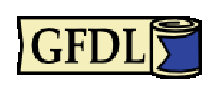
\includegraphics[width=1cm]{gfdl-logo-small.eps}
        \fi

Copyright (c) 2012  Laurent Claessens

Permission is granted to copy, distribute and/or modify this document under the terms of the \href{http://www.gnu.org/licenses/fdl-1.3.html}{GNU Free Documentation License}, Version 1.3 or any later version published by the Free Software Foundation; with no Invariant Sections, no Front-Cover Texts, and no Back-Cover Texts. A copy of the license is included in the chapter entitled ``GNU Free Documentation~License''.

\vspace{0.5cm}

Vous avez le droit de copier, distribuer et modifier ce document pourvu que vous suiviez les règles de la \wikipedia{fr}{GFDL}{GNU Free Documentation License}. Vous trouverez les sources \LaTeX\ sur gitorious :\\
    \url{https://www.gitorious.org/smath/smath/trees/master}

\end{center}


\newpage

% This is part of Un soupçon de mathématique sans être agressif pour autant
% Copyright (c) 2012-2013
%   Laurent Claessens
% See the file fdl-1.3.txt for copying conditions.

%+++++++++++++++++++++++++++++++++++++++++++++++++++++++++++++++++++++++++++++++++++++++++++++++++++++++++++++++++++++++++++
\section*{Sources et remerciements}
%+++++++++++++++++++++++++++++++++++++++++++++++++++++++++++++++++++++++++++++++++++++++++++++++++++++++++++++++++++++++++++

Ces notes sont rédigées pour mes classes de seconde, de première STMG et de terminale STL du lycée Jacques Duhamel ainsi que du lycée Jules Haag.

\begin{enumerate}
    \item
        Pour les statistiques descriptives, les fonctions et les systèmes d'équations, j'ai pompé énormément à Pauline Klein\footnote{Je tiens à préciser que sa mise en page était plus belle que celle que celle que vous trouverez ici.}. Je lui ai copié de nombreux exercices dans à peu près tous les chapitres.
    \item
        Certaines idées et définitions proviennent de \cite{oklaEg}.
    \item
        Certains exercices pour les STMG ont profité des exemples donnés par madame Colette Perrot (merci) 
    \item
        J'ai pris les fiches \cite{qyKnLf} sur les statistiques descriptives trouvées sur le site de l'université de Montpelier 3 (Paul Valéry). Je les copie ici avec l'aimable autorisation de Richard Varro.
    \item
        J'ai pris de nombreux exercices de questions posées sur le forum de l'\href{http://www.ilemaths.net/forum_lycee.php}{île des mathématiques}.
    \item
        Pas mal d'exercices proviennent de \href{http://tehessin.tuxfamily.org/?page=35}{Guillaume Connan} qui a aimablement tout mis sous une \href{http://guilde.jeunes-chercheurs.org/Guilde/Licence/ldl.html}{licence de documentation libre}.
    \item
        Les \href{http://eduscol.education.fr/cid49154/mentions-legales.html}{mentions légales} d'éduscol donnent les documents sous licence \href{http://creativecommons.org/licenses/by-nc-sa/2.0/fr/}{Créative Commons}. Je ne m'en suis pas privé. Merci à celles et ceux qui y ont mis des choses.
\end{enumerate}

    Les personnes citées dans la bibliographie ne sont pas responsables des erreurs et bêtises que j'ai pu introduire dans leurs énoncés en recopiant. J'ai souvent remanié, raccourci ou rallongé les exercices dont je me suis inspiré. Ne pas croire que les personnes citées ont écrit texto ce qui se retrouve ici.

%+++++++++++++++++++++++++++++++++++++++++++++++++++++++++++++++++++++++++++++++++++++++++++++++++++++++++++++++++++++++++++ 
%\section*{Note à propos des calculatrices}
%+++++++++++++++++++++++++++++++++++++++++++++++++++++++++++++++++++++++++++++++++++++++++++++++++++++++++++++++++++++++++++

%Est-ce que quelqu'un pourrait me dire si la proposition suivante est vraie ou fausse ?
%\begin{quote}
%    L'usage des calculatrices en classe est uniquement possible parce que TI et Casio sont en état de monopole. Si dix entreprises fournissaient dix modèles différents avec des modes opératoires différents, les cours à la calculatrices ne seraient pas possibles. En particulier, TI et Casio prennent l'éducation nationale comme un substitut à écrire des modes d'emploi lisibles, et vivent d'une sorte de taxe sur l'enseignement.

%    En un mot : elles sont des entreprises parasites de l'éducation nationale. (sans compter les déchets que génèrent toutes ces calculatrices)
%\end{quote}

%+++++++++++++++++++++++++++++++++++++++++++++++++++++++++++++++++++++++++++++++++++++++++++++++++++++++++++++++++++++++++++ 
\section*{Pour les élèves}
%+++++++++++++++++++++++++++++++++++++++++++++++++++++++++++++++++++++++++++++++++++++++++++++++++++++++++++++++++++++++++++

Les corrections données dans ce document ne sont pas complètes. Certaines se contentent de donner la réponse finale sans justifications, pour vous permettre de vous contrôler. Recopier mot à mot ce que vous trouvez ici sur une feuille de DM ne vous assure pas (très loin s'en faut) d'avoir une bonne note.

Conseil : les exercices corrigés sont le plus souvent des exercices qui sont arrivés dans des devoirs. Si ils sont arrivés une fois, il peuvent encore arriver.


\tableofcontents

\newpage

%&=& &=& &=& &=& &=& &=& &=& &=& &=& &=& &=& &=& &=& &=& &=& &=& &=& &=& &=& &=& &=& &=& &=& 
\part{Seconde}
%&=& &=& &=& &=& &=& &=& &=& &=& &=& &=& &=& &=& &=& &=& &=& &=& &=& &=& &=& &=& &=& &=& &=& 

\chapter{Repères, distances, milieux}
% This is part of Un soupçon de mathématique sans être agressif pour autant
% Copyright (c) 2012-2013
%   Laurent Claessens
% See the file fdl-1.3.txt for copying conditions.


%+++++++++++++++++++++++++++++++++++++++++++++++++++++++++++++++++++++++++++++++++++++++++++++++++++++++++++++++++++++++++++
\section{Repères et coordonnées}
%+++++++++++++++++++++++++++++++++++++++++++++++++++++++++++++++++++++++++++++++++++++++++++++++++++++++++++++++++++++++++++

%AFAIRE : installer geogebra.


Début de match sur un terrain faisant \unit{50}{\meter} de large et \unit{100}{\meter} de long. Le joueur \( A\) fait une passe à son attaquant \( B\). Ce dernier est situé \unit{10}{\meter} au-dessus de la ligne médiane et à \unit{5}{\meter} à gauche du bord du terrain.

\begin{center}
   \input{Fig_EGDFJAT.pstricks}
\end{center}

\begin{enumerate}
    \item
        Compléter le dessin.
    \item
        Quelle est la longueur de la passe ?
    \item
        L'attaquant veut directement tirer vers le but. À quelle distance est-il ?
\end{enumerate}
% Le rayon du cercle au centre est de 10m, mais c'est fait exprès que c'est pas donné.


\begin{definition}
    Un \defe{repère orthonormé}{repère!orthonormé} du plan est la donné de trois points \( O\), \( I\), \( J\) non alignés formant un triangle rectangle isocèle en  \( O\).
\end{definition}

\begin{definition}
    Un \defe{repère}{repère} (quelconque) du plan est la donnée de trois points \( (O,I,J)\) non alignés.

    Les deux axes sont les droites \( (OI)\) et \( (OJ)\). Les longueurs \( OI\) et \( OJ\) servent de graduation.
\end{definition}

%+++++++++++++++++++++++++++++++++++++++++++++++++++++++++++++++++++++++++++++++++++++++++++++++++++++++++++++++++++++++++++
\section{Distance entre deux points}
%+++++++++++++++++++++++++++++++++++++++++++++++++++++++++++++++++++++++++++++++++++++++++++++++++++++++++++++++++++++++++++

\begin{Aretenir}

\begin{wrapfigure}{r}{7.0cm}
   \vspace{-1.5cm}        % à adapter.
   \centering
   \input{Fig_PythagoreeBqLDU.pstricks}
\end{wrapfigure}

        Soient les points \( A\) et \( B\) de coordonnées \( A=(x_A,y_A)\) et \( B=(x_B,y_B)\) dans un repère orthonormé. La distance entre \( A\) et \( B\) est donnée par la formule
        \begin{equation*}
            AB =\sqrt{(x_B-x_A)^2+(y_B-y_A)^2}.
        \end{equation*}
    \end{Aretenir}

% Attention : cette démonstration n'est pas du tout à donner en classe. On met seulement l'illustration.
\begin{proof}
    Nous allons utiliser le théorème de Pythagore. Pour cela nous construisons le triangle rectangle construit sur les points \( A\) et \( B\) comme indiqué sur le dessin. Le point \( C\) est le point de même abscisse que \( B\) et de même ordonnée que \( A\), c'est à dire que \( C\) est le point
    \begin{equation}
        C=(x_B,y_A).
    \end{equation}
    La droite \( AC\) est parallèle à l'axe des abscisses et la droite \( BC\) est parallèle à l'axe des ordonnées; elles sont donc perpendiculaires et le triangle \( ABC\) est un triangle rectangle en \( C\). Le théorème de Pythagore s'applique :
    \begin{equation}    \label{EqjLjEKr}
       AB =\sqrt{ AC^2+BC^2}.
    \end{equation}
    Il reste à déterminer les longueurs \(  AC \) et \(  BC \). Le segment \( [AC]\) est horizontal et s'étend de l'abscisse \( x_A\) à l'abscisse \( x_B\), donc il est de longueur soit \( x_A-x_B\) soit \( x_B-x_A\), mais dans les deux cas nous avons
    \begin{equation}
         AC^2=(x_B-x_A)^2.
    \end{equation}
    De la même façon nous avons 
    \begin{equation}
         BC^2=(y_B-y_A)^2.
    \end{equation}
    En remplaçant dans \eqref{EqjLjEKr}, nous obtenons le résultat annoncé.
\end{proof}

%+++++++++++++++++++++++++++++++++++++++++++++++++++++++++++++++++++++++++++++++++++++++++++++++++++++++++++++++++++++++++++
\section{Milieu d'un segment}
%+++++++++++++++++++++++++++++++++++++++++++++++++++++++++++++++++++++++++++++++++++++++++++++++++++++++++++++++++++++++++++

\begin{Aretenir}
    Soient les points \( A\) et \( B\) de coordonnées \( A=(x_A;y_A)\) et \( B=(x_B;y_B)\) dans un repère. Alors le milieu du segment \( [AB]\) est le point de coordonnées
    \begin{equation*}
            \left( \frac{ x_A+x_B }{ 2 }\,;\,\frac{ y_A+y_B }{2} \right).
    \end{equation*}
\end{Aretenir}


%+++++++++++++++++++++++++++++++++++++++++++++++++++++++++++++++++++++++++++++++++++++++++++++++++++++++++++++++++++++++++++
\section{Compléments}
%+++++++++++++++++++++++++++++++++++++++++++++++++++++++++++++++++++++++++++++++++++++++++++++++++++++++++++++++++++++++++++

La façon dont nous associons à chaque point \( M\) du plan ses coordonnées dans le repère \( O\), \( I\), \( J\) est donnée à la figure \ref{LabelFigReperexjVyii}.
\newcommand{\CaptionFigReperexjVyii}{Lire les coordonnées du point \( M\) dans le repère \( OIJ\).}
\input{Fig_ReperexjVyii.pstricks}


%+++++++++++++++++++++++++++++++++++++++++++++++++++++++++++++++++++++++++++++++++++++++++++++++++++++++++++++++++++++++++++
\section{Exercices}
%+++++++++++++++++++++++++++++++++++++++++++++++++++++++++++++++++++++++++++++++++++++++++++++++++++++++++++++++++++++++++++


%---------------------------------------------------------------------------------------------------------------------------
\subsection{Placer et lire des coordonnées dans un repère}
%---------------------------------------------------------------------------------------------------------------------------

% Si tu veux un avis, je crois que ces exercices ne sont pas à mettre sur les feuilles distribuées.
\Exo{Seconde-0001}
\Exo{Seconde-0002}
\Exo{Seconde-0007}
\Exo{Seconde-0062}

%---------------------------------------------------------------------------------------------------------------------------
\subsection{Milieu de segments}
%---------------------------------------------------------------------------------------------------------------------------

\Exo{smath-0019}
\Exo{smath-0020}
\Exo{Seconde-0012}
\Exo{Seconde-0055}
\Exo{Seconde-0011}
\Exo{smath-0021}
\Exo{Seconde-0056}

%---------------------------------------------------------------------------------------------------------------------------
\subsection{Longueur de segments}
%---------------------------------------------------------------------------------------------------------------------------

\Exo{Seconde-0008}
\Exo{smath-0125}
\Exo{Seconde-0003}
\Exo{smath-0410}
\Exo{Seconde-0004}
\Exo{Seconde-0005}
\Exo{Seconde-0006}
\Exo{Seconde-0009}
\Exo{Seconde-0010}
\Exo{smath-0026}
\Exo{Seconde-0013}
\Exo{Seconde-0021}
\Exo{Seconde-0019}
\Exo{Seconde-0020}
\Exo{smath-0293}

%---------------------------------------------------------------------------------------------------------------------------
\subsection{Problèmes}
%---------------------------------------------------------------------------------------------------------------------------


\Exo{smath-0124}
\Exo{Seconde-0077}
\Exo{smath-0027}
\Exo{Seconde-0078}
\Exo{Seconde-0079}
\Exo{smath-0029}
\Exo{Seconde-0080}
\Exo{Seconde-0081}
\Exo{Seconde-0082}
\Exo{Seconde-0083}
\Exo{Seconde-0084}
\Exo{Seconde-0085}
\Exo{Seconde-0099}
\Exo{Seconde-0100}


\Exo{smath-0028}




\chapter{Fonctions : mode graphique}
%This is part of Un soupçon de mathématique sans être agressif pour autant
% Copyright (c) 2012-2014
%   Laurent Claessens
% See the file fdl-1.3.txt for copying conditions.

%+++++++++++++++++++++++++++++++++++++++++++++++++++++++++++++++++++++++++++++++++++++++++++++++++++++++++++++++++++++++++++ 
\section{Objectifs du chapitre}
%+++++++++++++++++++++++++++++++++++++++++++++++++++++++++++++++++++++++++++++++++++++++++++++++++++++++++++++++++++++++++++

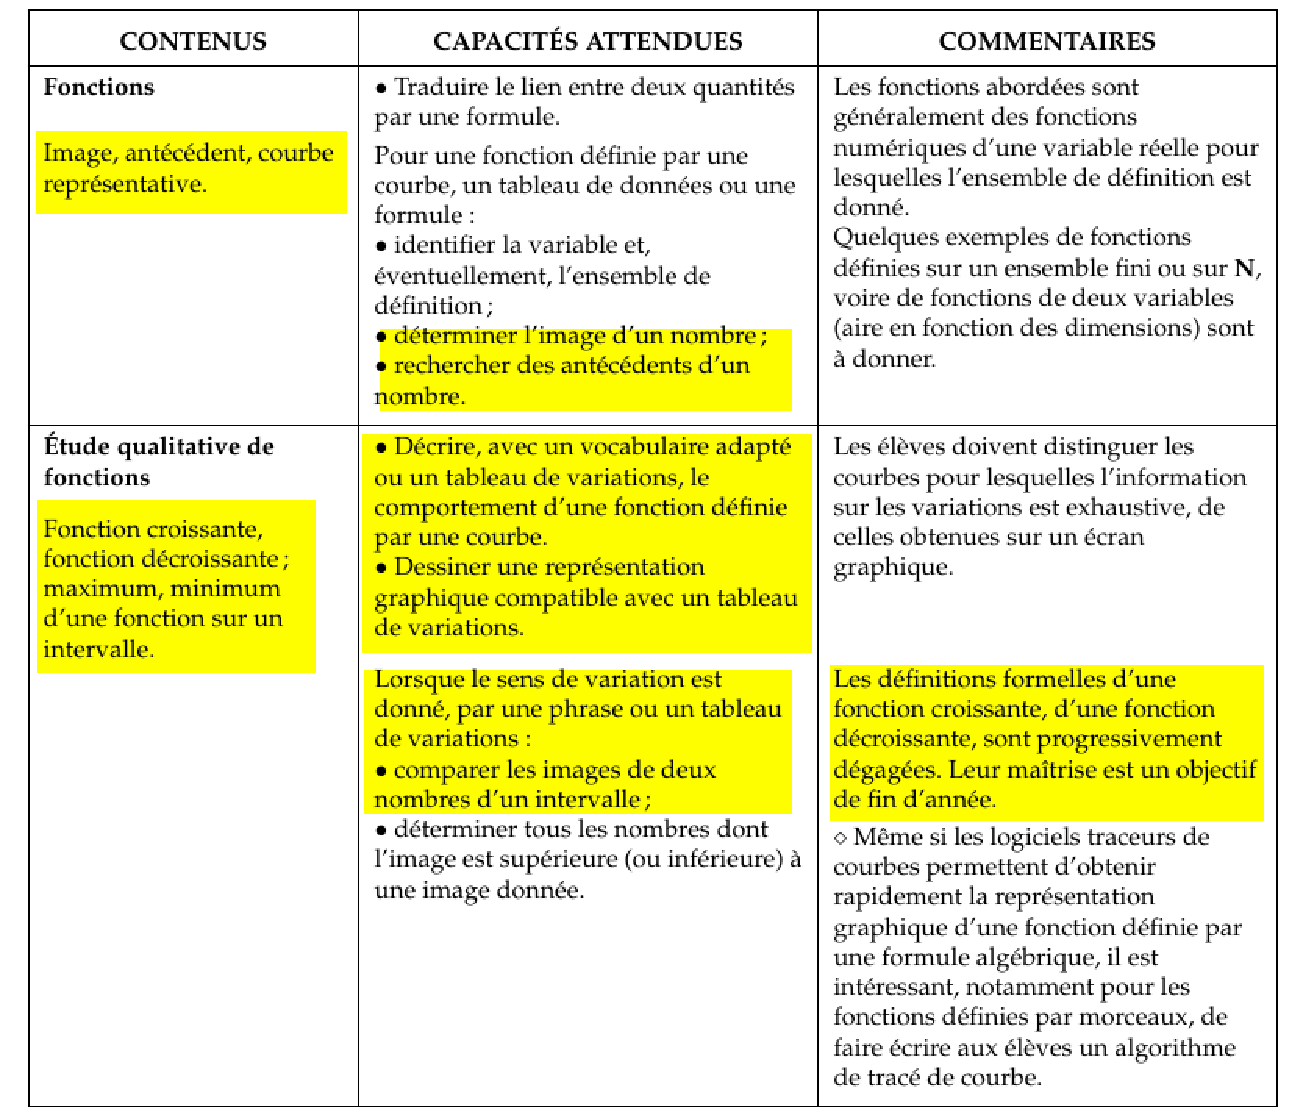
\includegraphics[width=\linewidth]{BO_fonctions_graphique.pdf}

%This is part of Un soupçon de mathématique sans être agressif pour autant
% Copyright (c) 2012-2013
%   Laurent Claessens
% See the file fdl-1.3.txt for copying conditions.

    Un berger syldave s'entraine pour le championnat national du lancer de chèvre. L'épreuve consiste à lancer une chèvre vers le haut depuis le bord d'une falaise située au bord d'un lac tranquille. La hauteur de la chèvre en fonction du temps par rapport à la surface du lac tranquille est une fonction \( f\) donnée par le graphique suivant.

    \begin{center}
        \input{Fig_WRXbDCo.pstricks}
    \end{center}
    La dernière partie du graphique correspond à la chèvre que l'on remonte rapidement hors de l'eau.
    À partir du graphique :
    \begin{enumerate}
        \item
            À quelle hauteur se trouve la chèvre au moment du lancer ?
        \item
            Pendant combien de temps la chèvre reste à une hauteur supérieure à celle à laquelle elle a été lancée ?
        \item
            À quel moment la chèvre atteint-elle sa hauteur maximale ? Quelle est cette hauteur ?
        \item
            À quelle hauteur se trouve la chèvre après \( 2.5\) secondes de vol ?
        \item
            Résumer toutes ces informations en dressant le tableau de variation de la fonction \( f\).
    \end{enumerate}


%+++++++++++++++++++++++++++++++++++++++++++++++++++++++++++++++++++++++++++++++++++++++++++++++++++++++++++++++++++++++++++
\section{Courbe représentative d'une fonction}
%+++++++++++++++++++++++++++++++++++++++++++++++++++++++++++++++++++++++++++++++++++++++++++++++++++++++++++++++++++++++++++


\begin{definition}
Soit $f$ une fonction définie sur un ensemble $\defD$.
    On appelle \defe{représentation graphique}{représentation graphique (d'une fonction)}, ou le \defe{graphe}{graphe} de $f$, l'ensemble des points $(x,y)$ tels que $x\in\defD$ et $y=f(x)$.

    Lorsque \( y=f(x)\), le nombre \( y\) est l'\defe{image}{image par une fonction} de \( x\) par la fonction \( f\) et \( x\) est \emph{un} \defe{antécédent}{antécédent} de \( y\).
\end{definition}

\begin{Aretenir}
    La règle d'or des graphiques : le point de coordonnées \( (a;b)\) est sur le graphique de la fonction \( f\) si et seulement si \( f(a)=b\).
\end{Aretenir}

\clearpage

\begin{multicols}{2}

À propos du graphe ci-contre :
\begin{enumerate}
    \item
        Quel est l'ensemble de définition de la fonction \( f\) ?
    \item
        Quelle est l'image de \( 1\) par \( f\) ?
    \item
        Donner un antécédent de \( 3\).
    \item
        Que vaut \( f(-3)\) ?
    \item
        Quels sont les antécédents de \( -1\) ?
    \item 
        Quel est le maximum de \( f\) sur \( \mathopen[ -2 , 1 \mathclose]\) ?
    \item
        Quel est le maximum de \( f\) sur \( \mathopen[ -2 , 2 \mathclose]\) ?
\end{enumerate}
    
    \columnbreak

\begin{center}
   \input{Fig_AHAbqhj.pstricks}
\end{center}

\end{multicols}

%+++++++++++++++++++++++++++++++++++++++++++++++++++++++++++++++++++++++++++++++++++++++++++++++++++++++++++++++++++++++++++ 
\section{Sens de variation, minimum et maximum}
%+++++++++++++++++++++++++++++++++++++++++++++++++++++++++++++++++++++++++++++++++++++++++++++++++++++++++++++++++++++++++++

\begin{definition}
      Soit $f$ une fonction définie sur un intervalle \( I\) de \( \eR\).
      \begin{enumerate}
          \item 
              On dit que $f$ est \defe{croissante}{croissante (fonction)} sur $I$ si pour tout choix de réels $a$ et $b$ dans $I$ tels que $a\leq b$ nous avons $f(a)\leq f(b)$.
    \item 
        On dit que $f$ est \defe{décroissante}{décroissante (fonction)} sur $I$ si pour tout choix de $a$ et $b$ dans $I$ tels que $a\leq b$, nous avons $f(a)\geq f(b)$. 
      \end{enumerate}
\end{definition}

Une fonction croissante range les images dans le même ordre que les antécédents. Une fonction décroissante inverse cet ordre. 

\begin{example}
    Nous considérons la fonction \( f\colon x\mapsto x^2\) sur \( \eR^+\).
    \begin{equation*}
        \begin{array}[]{|c||c|}
            \hline
            x&f(x)\\
            \hline\hline
            0&0\\
            \hline
            0.1&0.01\\
            \hline
            0.5&0.25\\
            \hline
            1&1\\
            \hline
            2&4\\
            \hline
            10&100\\
            \hline
        \end{array}
    \end{equation*}
    Dans ce tableau les valeurs de \( x\) sont rangées dans l'ordre croissant et nous remarquons que les images le sont aussi. La fonction \( f(x)=x^2\) est donc croissante tant qu'on considère des nombres positifs.

    Pour les valeurs négatives c'est le contraire :
    \begin{equation*}
        \begin{array}[]{|c||c|}
            \hline
            x&f(x)\\
            \hline\hline
            -10&100\\
            \hline
            -2&4\\
            \hline
            -1&1\\
            \hline
            -0.5&0.25\\
            \hline
            -0.1&0.01\\
            \hline
            0&0\\
            \hline
        \end{array}
    \end{equation*}
    Ici les antécédents sont dans l'ordre croissant et les images sont dans l'ordre décroissant.
\end{example}
  


Les notions de minima et maxima parlent, comme l'indiquent leurs noms en français, des points du graphe d'une fonction les plus hauts et les plus bas.

\begin{definition}
      Soit $f$ une fonction définie sur un intervalle \( I\).
      \begin{itemize}
            \item 
                Nous disons que le réel \( M\) est le \defe{maximum}{maximum} de \( f\) sur $I$ si et seulement si 
                \begin{enumerate}
                    \item
                        il existe $ a\in I$ tel que $f(a)=M$,
                    \item
                        \( f(x)\leq M\) pour tout $x\in I$.
                \end{enumerate}
                
          \item 
                Nous disons que le réel \( m\) est le \defe{minimum}{minimum} de \( f\) sur $I$ si et seulement si
                \begin{enumerate}
                    \item
                        il existe $ b\in I$ tel que $f(b)=m$,
                    \item
                        $f(x)\geq m$ pour tout \( x\in I\).
                \end{enumerate}
      \end{itemize}
\end{definition}

\begin{center}
   \input{Fig_MinMaxKNRdOd.pstricks}
\end{center}

\begin{remark}
    Attention à deux choses.
    \begin{enumerate}
        \item
            Le minimum est la \emph{valeur} la plus basse, et non l'abscisse correspondante. Idem pour le maximum. 
        \item
            La minimum dépend de l'intervalle sur lequel on regarde la fonction.
    \end{enumerate}
\end{remark}

Une illustration sur la figure ci-contre. La fonction prend son maximum en \( x=a\) et ce maximum vaut \( M\). La fonction prend son minimum en \( x=b\) et ce minimum vaut \( m\).



\chapter{Fonctions affines et linéaires}
%This is part of Un soupçon de mathématique sans être agressif pour autant
% Copyright (c) 2012-2013
%   Laurent Claessens, Pauline Klein
% See the file fdl-1.3.txt for copying conditions.

%+++++++++++++++++++++++++++++++++++++++++++++++++++++++++++++++++++++++++++++++++++++++++++++++++++++++++++++++++++++++++++ 
\section{Définitions}
%+++++++++++++++++++++++++++++++++++++++++++++++++++++++++++++++++++++++++++++++++++++++++++++++++++++++++++++++++++++++++++

\begin{definition}
    Une \defe{fonction affine}{affine}\index{fonction!affine} est une fonction définie sur \( \eR\) par
    \begin{equation}
        f(x)=ax+b
    \end{equation}
    où \( a\) et \( b\) sont deux nombres réels fixés.
\end{definition}

Cas particuliers :
\begin{enumerate}
    \item
        Si \( b=0\) alors \( f(x)=ax\) et nous disons que \( f\) est une fonction \defe{linéaire}{fonction!linéaire}.
    \item
        Si \( a=0\) alors \( f(x)=b\) et nous disons que \( f\) est une fonction \defe{constante}{fonction!constante}.
\end{enumerate}

%---------------------------------------------------------------------------------------------------------------------------
\subsection{Fonctions linéaires et affines}
%---------------------------------------------------------------------------------------------------------------------------

\begin{definition}
    Une classe importante de fonctions sont les fonctions de la forme \( f(x)=ax\) où \( a\) est un nombre. Une telle fonction est dite \defe{linéaire}{linéaire (fonction)}. 

    Les fonctions du type \( f(x)=ax+b\) sont des fonctions \defe{affines}{affine (fonction)}. 
\end{definition}


\begin{Aretenir}
    Les fonctions linéaires et affines sont très importantes parce que leur graphe sont des droites. 
    \begin{itemize}
        \item 
    Les fonctions linéaires sont des droites qui passent par l'origine \( (0;0)\).
    \item
    Les fonctions affines (avec \( b\neq 0\)) sont des droites ne passant pas par \( (0;0)\).
    \end{itemize}
\end{Aretenir}
Si $f$ est une fonction affine définie pour $x\in\eR$ par $f(x)=ax+b$ alors l'équation de la droite représentative de la fonction est $y=ax+b$. 

Pour tracer le graphe d'une fonction affine.
\begin{itemize}
    \item
        Vu que le graphe est une droite, il suffit de deux points.
    \item
        Les fonction linéaires passent par l'origine \( (0;0)\).
    \item 
        Pour un tracé à la règle, il est plus précis de prendre deux points relativement éloignés.
    \item
        La droite \( f(x)=ax+b\) monte si \( a>0\) et descend si \( a<0\). La pente est d'autant plus raide que \( a\) est grand.
\end{itemize}

Quelque exemples à la figure \ref{LabelFigGrapheAffinHqXJGx}.
\newcommand{\CaptionFigGrapheAffinHqXJGx}{Des graphes de fonctions linéaires et affines.}
\input{Fig_GrapheAffinHqXJGx.pstricks}

%+++++++++++++++++++++++++++++++++++++++++++++++++++++++++++++++++++++++++++++++++++++++++++++++++++++++++++++++++++++++++++ 
\section{Représentation graphique}
%+++++++++++++++++++++++++++++++++++++++++++++++++++++++++++++++++++++++++++++++++++++++++++++++++++++++++++++++++++++++++++

\begin{Aretenir}
    La représentation graphique de la fonction \( f(x)=ax+b\) est une droite non parallèle à l'axe des ordonnées. Réciproquement toute droite non parallèle est la représentation graphique d'une fonction affine.
\end{Aretenir}

Si \( f(x)=ax+b\), alors nous avons \( f(0)=b\), ce qui signifie que \( b\) est la hauteur de la droite au-dessus de l'origine.

En ce qui concerne le signification du coefficient \( a\), nous traçons quelque droites.


\begin{remark}
    Demander aux élèves de faire ces dessins eux-mêmes.
\end{remark}

\newpage

\begin{multicols}{2}
    Sur la figure ci-contre, nous avons tracé les droites
    \begin{enumerate}
        \item
            \( f(x)=2x+1\)
        \item
            \( g(x)=2x-2\)
        \item
            \( h(x)=3x-1\)
    \end{enumerate}

    \columnbreak

%The result is on figure \ref{LabelFigfigureCFoZCYe}. % From file figureCFoZCYe
%\newcommand{\CaptionFigfigureCFoZCYe}{<+Type your caption here+>}
    \begin{center}
\input{Fig_figureCFoZCYe.pstricks}
    \end{center}

\end{multicols}

Nous constatons que
\begin{enumerate}
    \item
        Les droites représentatives de \( f\) et \( g\) sont parallèles.
    \item
        La droite \( h\) est plus pendue que les deux autres.
\end{enumerate}

\begin{definition}
    Soit une droite \( d\) d'équation \( y=ax+b\). Le nombre \( a\) est appelé le \defe{coefficient directeur}{coefficient directeur} de la droite.
\end{definition}



Un exemple des éléments de \( ax+b\) est donné à la figure \ref{LabelFigfigureUERGVgS}. % From file figureUERGVgS
\newcommand{\CaptionFigfigureUERGVgS}{Une droite et quelque éléments de son équation.}
\input{Fig_figureUERGVgS.pstricks}

\begin{propriete}
    Soit \( f(x)=ax+b\) une fonction affine.
    \begin{enumerate}
        \item
            Si \( a>0\) alors \( f\) est croissante sur \( \eR\).
        \item
            Si \( a<0\) alors \( f\) est décroissante sur \( \eR\).
        \item
            Si \( a=0\) alors \( f\) est constante sur \( \eR\) (et vaut \( b\)).
    \end{enumerate}
\end{propriete}


\begin{theorem}
    Soit la fonction affine \( f(x)=ax+b\). Alors pour tout nombres distincts \( u\) et \( v\) nous avons
    \begin{equation}
        \frac{ f(u)-f(v) }{ u-v }=a.
    \end{equation}
\end{theorem}

\begin{proof}
    Soient \( u\) et \( v\), deux réels distincts. Nous calculons
    \begin{equation}
        f(u)-f(v)=au+b-(av+b)=au-av=a(u-v).
    \end{equation}
    En divisant par \( u-v\) on trouve le résultat annoncé.
\end{proof}

Cela donne une méthode graphique pour déterminer le coefficient directeur d'une droite. Si les points \( A=(x_A;y_A)\) et \( B=(x_B;y_B)\) sont sur la droite \( d\) d'équation \( y=ax+b\), alors
\begin{equation}
    a=\frac{ y_B-y_A }{ x_B-x_A }.
\end{equation}
Notez que cela vient du vecteur directeur
\begin{equation}
    \begin{pmatrix}
        x_B-x_A    \\ 
        y_B-y_A    
    \end{pmatrix}
\end{equation}


\subsection{Sens de variation d'une fonction affine}

\begin{Aretenir}
      Soit $f$ la fonction affine $x\mapsto ax+b$.
      \begin{itemize}
      \item Si $a>0$, alors $f$ est croissante sur $\eR$.
      \item Si $a<0$, alors $f$ est décroissante sur $\eR$.
      \item Si $a=0$, alors $f$ est constante sur $\eR$
        (et $f(x)=b$ pour tout $x\in\eR$).
      \end{itemize}
\end{Aretenir}
Nous savons que si \( f(x)=ax+b\), alors \( f\) s'annule en \( x=-\frac{ b }{ a }\). Cela nous sert à écrire un tableau de signe de \( f\).



Les figures \ref{LabelFigFnAffineipcEQfssLabelSubFigFnAffineipcEQf0} et \ref{LabelFigFnAffineipcEQfssLabelSubFigFnAffineipcEQf1} montrent des droites affines. Lorsque \( a>0\), la droite monte; lorsque \( a<0\) elle descend. La pente est d'autant plus forte que \( a\) est grand.
\newcommand{\CaptionFigFnAffineipcEQf}{Deux droites affines.}
\input{Fig_FnAffineipcEQf.pstricks}


\begin{Aretenir}
      Règle du signe de $ax+b$ \\
      
      \begin{tabular}{cc}
        $a<0$ & $a>0$ \\
        & \\
        $\begin{array}{|c|ccccc|}
          \hline
          x & -\infty & & -\dfrac{b}{a} & & +\infty \\[2ex]
          \hline
          ax+b & & + \quad \ & 0 & \quad - & \\[1ex]
          \hline
        \end{array}$
        &
        $\begin{array}{|c|ccccc|}
          \hline
          x & -\infty & & -\dfrac{b}{a} & & +\infty \\[2ex]
          \hline
          ax+b & & - \quad \ & 0 & \quad + & \\[1ex]
          \hline
        \end{array}$ \\
      \end{tabular}  \\[1ex] 
\end{Aretenir}



%+++++++++++++++++++++++++++++++++++++++++++++++++++++++++++++++++++++++++++++++++++++++++++++++++++++++++++++++++++++++++++ 
\section{Tableau de variation}
%+++++++++++++++++++++++++++++++++++++++++++++++++++++++++++++++++++++++++++++++++++++++++++++++++++++++++++++++++++++++++++

Nous savons qu'une fonction affine est croissante ou décroissante suivant le signe de \( a\). Il y a donc deux tableaux possibles. Les tableaux de signes s'en déduisent immédiatement.

\begin{minipage}{0.485\textwidth}
    \begin{center}

        Si \( a<0\)
        \vspace{5mm}

               \input{Fig_OSQOqJN.pstricks}   

               \begin{equation*}
                   \begin{array}[]{c|ccccc}
                        x&-\infty&&-b/a&&\infty\\
                         \hline
                         ax+b&&-&0&+&\\ 
                          \end{array}
                      \end{equation*}
    \end{center}
\end{minipage}
\hspace{1mm}
\begin{minipage}{0.485\textwidth}
    \begin{center}
        Si \( a>0\)
        \vspace{5mm}

                    \input{Fig_BZqEWco.pstricks}

               \begin{equation*}
                   \begin{array}[]{c|ccccc}
                        x&-\infty&&-b/a&&\infty\\
                         \hline
                         ax+b&&+&0&-&\\ 
                          \end{array}
                      \end{equation*}
    \end{center}
\end{minipage}


%+++++++++++++++++++++++++++++++++++++++++++++++++++++++++++++++++++++++++++++++++++++++++++++++++++++++++++++++++++++++++++ 
\section{Droites parallèles et droites sécantes}
%+++++++++++++++++++++++++++++++++++++++++++++++++++++++++++++++++++++++++++++++++++++++++++++++++++++++++++++++++++++++++++

%--------------------------------------------------------------------------------------------------------------------------- 
\subsection{Critère avec le coefficient directeur}
%---------------------------------------------------------------------------------------------------------------------------

\begin{example}
    Les droites \( y=-3x+4\) et \( y=2x+1\) sont sécantes, comme nous pouvons le voir sur un dessin. Comment trouver les coordonnées du point d'intersection ?

    Le point d'intersection \( (x_0;y_0)\) doit satisfaire \( y_0=-3x_0+4\) et \( y_0=2x_0+1\) en même temps. Donc
    \begin{equation}
        -3x_0+4=2x_0+1,
    \end{equation}
    ce qui donne \( x_0=\frac{ 3 }{ 5 }\). Pour trouver \( y_0\) il suffit de remplacer dans l'une ou l'autre équation :
    \begin{equation}
        y_0=-3x_0+4=-3\frac{ 3 }{ 5 }+4=\frac{ 11 }{ 5 }.
    \end{equation}
    Vérification : dans l'autre on obtient le même résultat :
    \begin{equation}
        y_0=2x_0+1=2\frac{ 3 }{ 5 }+1=\frac{ 11 }{ 5 }.
    \end{equation}
    Donc le point d'intersection des deux droites est le point de coordonnées
    \begin{equation}
        \big( \frac{ 3 }{ 5 };\frac{ 11 }{ 5 } \big).
    \end{equation}
\end{example}

\begin{theorem}
    Dans un repère, les droites d'équations \( y=ax+b\) et \( y=a'x+b'\) sont parallèles si et seulement si elles ont même coefficient directeur, c'est à dire si et seulement si \( a=a'\).

    Les droites sont sécantes si et seulement si \( a\neq a'\).
\end{theorem}

\begin{proof}
    Nous allons seulement démontrer que si \( a\neq a'\), alors les droites s'intersectent. Pour cela nous allons montrer qu'il existe un point \( (x_0,y_0)\) qui se trouve sur le graphe des deux fonctions, c'est à dire qui vérifie
    \begin{subequations}
        \begin{numcases}{}
            y_0=ax_0+b\\
            y_0=a'x_0+b'.
        \end{numcases}
    \end{subequations}
    Le nombre \( x_0\) doit donc satisfaire
    \begin{equation}
        ax_0+b=a'x_0+b',
    \end{equation}
    c'est à dire \( (a-a')x_0=b'-b\) et donc
    \begin{equation}
        x_0=\frac{ b'-b }{ a-a' }.
    \end{equation}
\end{proof}

%--------------------------------------------------------------------------------------------------------------------------- 
\subsection{Et le vecteur directeur}
%---------------------------------------------------------------------------------------------------------------------------

Si \( A\) et \( B\) sont des points du plan, nous avons déjà vu que le vecteur \( \vect{ AB }\) était un critère de parallélisme de la droite \( AB\). Plus précisément, nous avons vu qu'une droite \( (CD)\) était parallèle à \( AB\) si et seulement si \( \vect{ CD }\) est un multiple de \( \vect{ AB }\). Voyons cela de plus près.

Soit la droite \( y=ax+b\). Les points \( A=(0;b)\) et \( B=(1,a+b)\) sont sur cette droite et donc le vecteur directeur est
\begin{equation}
    \vect{ AB }=\begin{pmatrix}
        1    \\ 
        a    
    \end{pmatrix}
\end{equation}
Si les points \( C\) et \( D\) sont tels que \( (CD)\parallel (AB)\), alors
\begin{equation}
    \vect{ CD }=\lambda\begin{pmatrix}
        1    \\ 
        a    
    \end{pmatrix}=\begin{pmatrix}
        \lambda    \\ 
            \lambda a
    \end{pmatrix}.
\end{equation}
Si le point \( C\) a pour coordonnées \( C=(x_C;y_C)\), alors le point \( D\) doit avoir comme coordonnées
\begin{equation}
    D=\big( x_C+\lambda;y_C+\lambda a \big).
\end{equation}
Le coefficient directeur de la droite \( (CD)\) est alors
\begin{equation}
    \frac{ (y_C+\lambda a)-y_C }{ (x_C+\lambda)-x_C }=a.
\end{equation}
Nous avons donc confirmé que le critère du vecteur proportionnel et le critère du coefficient directeur sont en réalité les mêmes.

%+++++++++++++++++++++++++++++++++++++++++++++++++++++++++++++++++++++++++++++++++++++++++++++++++++++++++++++++++++++++++++ 
\section{Colinéarité}
%+++++++++++++++++++++++++++++++++++++++++++++++++++++++++++++++++++++++++++++++++++++++++++++++++++++++++++++++++++++++++++

\begin{theorem}
    Trois points distincts \( A\), \( B\) et \( C\) sont alignés si et seulement si les droites \( (AB)\) et \( (AC)\) ont même coefficient directeur.
\end{theorem}

\begin{proof}
    Si les droites \( (AB)\) et \( (AC)\) ont même coefficient directeur, alors nous pouvons écrire
    \begin{equation}
        (AB)\equiv y=ax+b
    \end{equation}
    et
    \begin{equation}
        (AC)\equiv ax+b'.
    \end{equation}
    Cependant \( A\) est un point commun aux deux droites : \( y_A=ax_A+b=ax_A+b'\) et donc \( b=b'\), ce qui signifie que les droites \( (AB)\) et \( (AC)\) sont les mêmes.
\end{proof}

\begin{example}
    Vérifions que les points \( A=(1;-1)\), \( B=(3;5)\) et \( C=(4;8)\) sont alignés.

    D'abord le coefficient directeur de la droite \( (AB)\) est 
    \begin{equation}
        \frac{ y_B-y_A }{ x_B-x_A }=\frac{ 5-(-1) }{ 3-1 }=3
    \end{equation}
    ensuite le coefficient directeur de la droite \( (AC)\) est
    \begin{equation}
        \frac{ y_C-y_A }{ x_C-x_A }=\frac{ 8+1 }{ 4-1 }=3
    \end{equation}
    Donc les points \( A\), \( B\) et \( C\) sont alignés.
\end{example}

%+++++++++++++++++++++++++++++++++++++++++++++++++++++++++++++++++++++++++++++++++++++++++++++++++++++++++++++++++++++++++++ 
\section{Exercices}
%+++++++++++++++++++++++++++++++++++++++++++++++++++++++++++++++++++++++++++++++++++++++++++++++++++++++++++++++++++++++++++

%---------------------------------------------------------------------------------------------------------------------------
\subsection{Équations linéaires et affines}
%---------------------------------------------------------------------------------------------------------------------------

\Exo{smath-0016}

%--------------------------------------------------------------------------------------------------------------------------- 
\subsection{Équations de droites}
%---------------------------------------------------------------------------------------------------------------------------

\Exo{smath-0154}
\Exo{smath-0330}        % Cet exo est le même que le smath-155, mais en plus court pour rentrer dans un devoir.
\Exo{smath-0344}
\Exo{smath-0128}
\Exo{smath-0149}
\Exo{smath-0409}    % presque le même que le smath-0149, mais plus court pour un DS.
\Exo{smath-0130}
\Exo{smath-0069}
\Exo{smath-0394}
\Exo{smath-0229}    % Le même que smath-0413, mais en plus guidé pour un DS.
\Exo{smath-0135}
\Exo{smath-0413}
\Exo{smath-0150}    
\Exo{smath-0155}
\Exo{smath-0151}
\Exo{smath-0134}
\Exo{smath-0086}
\Exo{smath-0138}
\Exo{smath-0200}
\Exo{smath-0233}
\Exo{smath-0234}
\Exo{smath-0153}
\Exo{Seconde-0019}

%--------------------------------------------------------------------------------------------------------------------------- 
\subsection{Tableaux de variation et de signe}
%---------------------------------------------------------------------------------------------------------------------------

\Exo{smath-0132}
\Exo{smath-0148}
\Exo{smath-0321}

%---------------------------------------------------------------------------------------------------------------------------
\subsection{Parallélisme et intersection}
%---------------------------------------------------------------------------------------------------------------------------

%TODO : écrire un exercice avec un rebond sur une table de billard.
\Exo{smath-0083}
\Exo{smath-0129}
\Exo{smath-0110}    % TODO: il faut plus d'exercices comme celui-ci.
\Exo{smath-0084}

\Exo{smath-0235}
\Exo{smath-0236}
\Exo{smath-0237}
\Exo{smath-0239}
\Exo{smath-0345}
\Exo{smath-0451}
\Exo{smath-0450}


%--------------------------------------------------------------------------------------------------------------------------- 
\subsection{Problèmes}
%---------------------------------------------------------------------------------------------------------------------------

\Exo{smath-0241}
\Exo{smath-0242}


\chapter{Statistique descriptive}
% This is part of Un soupçon de mathématique sans être agressif pour autant
% Copyright (c) 2012-2013
%   Laurent Claessens, Pauline Klein
% See the file fdl-1.3.txt for copying conditions.

\EpsOrPdfincludegraphics[width=\linewidth]{BO_statistique_descriptive}

\setcounter{section}{-1}
%+++++++++++++++++++++++++++++++++++++++++++++++++++++++++++++++++++++++++++++++++++++++++++++++++++++++++++++++++++++++++++ 
\section{Activité : un peu de spam ?}
%+++++++++++++++++++++++++++++++++++++++++++++++++++++++++++++++++++++++++++++++++++++++++++++++++++++++++++++++++++++++++++

% This is part of Un soupçon de mathématique sans être agressif pour autant
% Copyright (c) 2013
%   Laurent Claessens
% See the file fdl-1.3.txt for copying conditions.

% ATTENTION : les chiffres donnés ici sont repris dans le cours au moment des ECC.

\begin{wrapfigure}[5]{r}{8cm}
   \vspace{-0.5cm}        % à adapter.
   \centering
   \input{Fig_YRQOoPE.pstricks}
\end{wrapfigure}

Le graphique ci-contre illustre le nombre de spam reçus aujourd'hui par les élèves d'une classe.
\begin{enumerate}
    \item
        Combien d'élèves y-a-t-il dans la classe ?
    \item
        Combien d'élèves ont reçu \( 5\) spams ou plus ?
    \item
        En moyenne combien de spam ont reçu les élèves aujourd'hui ?
    \item
        Diviser la classe en 4 groupes suivant le nombre de spams reçus.
\end{enumerate}



Éléments de réponse.

\begin{enumerate}
    \item
Nous pouvons remplir le tableau
\begin{equation*}
    \begin{array}[]{|c||c|c|c|c|c|c|c|c|c|c|c|| c |}
        \hline
        \text{Nombre}&1&2&3&4&5&6&7&8&9&10&11&\text{total}\\
        \hline\hline
        \text{Effectifs}&3&0&1&4&4&2&1&5&3&1&1&25\\
        \hline
    \end{array}
\end{equation*}
\item
Il y a \( 17\) élèves ayant reçu \( 5\) spams ou plus.
     \item
         Pour calculer la moyenne il faut d'abord calculer le nombre total de spams reçus, puis diviser par le nombre d'élèves :
         \begin{equation}
             \text{moyenne}=\frac{ 3\times 1+1\times 3+4\times 4+4\times 5+2\times 6+\ldots+1\times 11 }{ 25 }=\frac{ 149 }{ 25 }=5.96.            
         \end{equation}
     \item
         En ce qui concerne la division de la classe en quatre groupe, vu que \( 25\) n'est pas divisible en \( 4\), il va falloir donner une convention sur les arrondis.
\end{enumerate}

%+++++++++++++++++++++++++++++++++++++++++++++++++++++++++++++++++++++++++++++++++++++++++++++++++++++++++++++++++++++++++++ 
\section{Les quartiles et la médiane}
%+++++++++++++++++++++++++++++++++++++++++++++++++++++++++++++++++++++++++++++++++++++++++++++++++++++++++++++++++++++++++++

\begin{definition}
    Nous considérons une liste de \( n\) valeurs triées par ordre croissant (avec éventuellement les répétitions).
    \begin{enumerate}
        \item
            La \defe{médiane}{médiane}, est la valeur qui sépare la liste en deux parties égales. C'est le terme du milieu si l'effectif total est impair et la moyenne des deux termes du milieu si l'effectif total est pair.
      \item 
          Le \defe{premier quartile}{quartile!premier} $Q_1$ est la plus petite valeur de la liste telle qu'au moins un quart des valeurs de la liste soient inférieures ou égales à $Q_1$.
        \item
            Le \defe{troisième quartile}{quartile!troisième} $Q_3$ est la plus petite valeur de la liste telle qu'au moins les trois quarts des valeurs de la liste soient inférieures ou égales à $Q_3$.
  \end{enumerate}
\end{definition}
En pratique :
\begin{itemize}
    \item 
  Pour le calcul de $Q_1$, on calcule $\dfrac{n}4$, puis on détermine le premier entier $p$ supérieur ou égal à $\dfrac{n}4$. Cet entier $p$ donne le rang de $Q_1$. 
  \item
  Pour le calcul de $Q_3$, on fait de même en remplaçant $\dfrac{n}4$ par $\dfrac{3n}4$. 
\end{itemize}


\begin{example}

    Un laboratoire expérimente un médicament sur dix souris. Voici les temps (en semaines) que les souris ont encore vécu après l'injection : \( 2\), \( 5\), \( 10\), \( 2\), \( 1\), \( 3\), \( 10\), \( 5\), \( 5\), \( 1\).

    D'abord nous trions par ordre croissant en respectant les répétitions :
    \begin{equation*}
        \begin{array}[]{|c||c|c|c|c|c|c|c|c|c|c|}
            \hline
            \text{numéro de la souris}&1&2&3&4&5&6&7&8&9&10\\
            \hline
            \text{semaines de vie}&1&1&2&2&3&5&5&5&10&10\\
            \hline
        \end{array}
    \end{equation*}

    Il y a \( 10\) valeurs, donc 
    \begin{enumerate}
        \item
            Pour le premier quartile, \( \frac{ 10 }{ 4 }\simeq 2.5\), on prend la troisième valeur : \( Q_1=2\).
        \item
            Pour le troisième quartile, \( \frac{ 3}{ 4 }\times 10\simeq 7.5\), on prend la huitième valeur : \( Q_3=5\).
        \item
            Pour la médiane, on prend la moyenne entre la cinquième et la sixième valeur : \( \frac{ 3+5 }{2}=4\) : \( Med=4\).
    \end{enumerate}

    Nous résumons ces informations sur le diagramme suivant :


    \begin{center}
        \input{Fig_DNYAefI.pstricks}
    \end{center}


    Attention : nouvelle de dernière minute. Le laboratoire s'est trompé dans ses résultats. En réalité les deux souris qui ont vécu \( 10\) semaines ont vécu respectivement \( 15\) et \( 20\) semaines. Est-ce que ça change quelque chose ?

\end{example}

Avec ces définitions de quartile et de médiane, nous avons la distribution suivante :

\begin{center}
   \input{Fig_KDtwIJf.pstricks}
\end{center}

\section{Représentation graphique d'une série statistique}

%--------------------------------------------------------------------------------------------------------------------------- 
\subsection{Effectifs cumulés croissants}
%---------------------------------------------------------------------------------------------------------------------------

Nous classons les élèves d'une classe d'après la première lettre de leur noms. Le résultat est le tableau
\begin{center}
\begin{tabular}[]{|c||c|c|c|c|c|c|c|c|c|c|c|c||c|}
        \hline
        Lettre&a&b&c&d&h&j&l&m&p&r&s&t&total\\
        \hline\hline
        Effectifs&4&8&9&2&2&1&1&2&2&1&1&2&35\\
        \hline
        ECC&4&12&21&23&25&26&27&29&31&32&33&35&\\
        \hline
\end{tabular}
\end{center}

\input{Fig_MAXkaGz.pstricks}

Reprenons l'exemple du spam
\begin{equation*}
    \begin{array}[]{|c||c|c|c|c|c|c|c|c|c|c|c|| c |}
        \hline
        \text{Nombre}&1&2&3&4&5&6&7&8&9&10&11&\text{total}\\
        \hline
        \text{Effectifs}&3&0&1&4&4&2&1&5&3&1&1&25\\
        \hline
        \text{ECC}&3&3&4&8&12&14&15&20&23&24&25&\\
        \hline
    \end{array}
\end{equation*}

\begin{Aretenir}
    \begin{enumerate}
        \item
            Les effectifs cumulés croissants s'obtiennent en additionnant successivement les effectifs.
        \item
            La différence des ordonnées entre deux points successifs du graphe des ECC donne l'effectif correspondant à l'abscisse du deuxième point.
    \end{enumerate}
\end{Aretenir}

%--------------------------------------------------------------------------------------------------------------------------- 
\subsection{Graphe des fréquences cumulées croissantes}
%---------------------------------------------------------------------------------------------------------------------------

\begin{definition}
    La \defe{fréquence}{fréquence} d'une valeur est le rapport
    \begin{equation}
        \frac{ \text{effectif de la valeur} }{ \text{effectif total} }.
    \end{equation}
\end{definition}

\begin{Aretenir}
    La fréquence est un nombre entre \( 0\) et \( 1\). Le zéro correspond à «personne» et le \( 1\) correspond à «tout le monde».
\end{Aretenir}

Nous reprenons l'exemple du spam
\begin{equation*}
    \begin{array}[]{|c||c|c|c|c|c|c|c|c|c|c|c|| c |}
        \hline
        \text{Nombre}&1&2&3&4&5&6&7&8&9&10&11&\text{total}\\
        \hline\hline
        \text{Effectifs}&3&0&1&4&4&2&1&5&3&1&1&25\\
        \hline
        \text{Fréquences}&\hphantom{0.001}&\hphantom{0.001}&\hphantom{0.001}&\hphantom{0.001}&\hphantom{0.001}&\hphantom{0.001}&\hphantom{0.001}&\hphantom{0.001}&\hphantom{0.001}&\hphantom{0.001}&\hphantom{0.001}&\hphantom{0.001}\\
        \hline
        \text{FCC}&&&&&&&&&&&&\\
        \hline
    \end{array}
\end{equation*}

Le résultat est :
\begin{equation*}
    \begin{array}[]{|c||c|c|c|c|c|c|c|c|c|c|c|| c |}
        \hline
        \text{Nombre}&1&2&3&4&5&6&7&8&9&10&11&\text{total}\\
        \hline\hline
        \text{Effectifs}&3&0&1&4&4&2&1&5&3&1&1&25\\
        \hline
        \text{Fréquences}&0.12&0&0.04&0.16&0.16&0.08&0.04&0.2&0.12&0.04&0.04&1\\
        \hline
        \text{FCC}&0.12&0.12&0.16&0.32&0.48&0.56&0.6&0.8&0.92&0.96&1&\\
        \hline
    \end{array}
\end{equation*}
Attention : le total risque de ne pas tomber sur \( 1\) à cause des arrondis faits un peu partout.

\begin{center}
\input{Fig_FWyrYhJ.pstricks}
\end{center}

\begin{remark}
    Le total des fréquences doit faire \( 1\). Le dernier point du graphe des fréquence cumulées croissantes est donc d'ordonnée \( 1\).

    Des erreurs d'arrondis dans dans le calcul des fréquences peuvent entrainer que la somme ne vaut pas \( 1\).

    En pratique, pour dessiner le graphe des FCC il vaut mieux calculer les ECC puis les fréquences correspondantes, et non les fréquences et additionner.

\end{remark}

%--------------------------------------------------------------------------------------------------------------------------- 
\subsection{Histogramme}
%---------------------------------------------------------------------------------------------------------------------------

%TODO : c'est mieux de ne pas parler d'histogrammes à pas constant, mais directement de pas non constant et de montrer un exemple  qui tombe bien sur le quadrillage.

%///////////////////////////////////////////////////////////////////////////////////////////////////////////////////////////
\subsubsection{Le problème}
%///////////////////////////////////////////////////////////////////////////////////////////////////////////////////////////

Si nous regardons le chiffre d'affaire d'entreprises, il y a peu de chances que l'effectif de entreprises dont le chiffre d'affaire est exactement \( 14.258.736\)€ soit grand. Supposons avoir les nombres
\begin{center}
    100,101,105,502,503.
\end{center}
Il est immédiatement visible qu'il y a un paquet autour entre \( 100\) et \( 200\) et un paquet autour entre \( 500\) et \( 600\)a. Pourtant tracer le graphe des effectifs n'est pas très instructif :
\begin{center}
   \input{Fig_JXWXdJI.pstricks}
\end{center}

%///////////////////////////////////////////////////////////////////////////////////////////////////////////////////////////
\subsubsection{La solution}
%///////////////////////////////////////////////////////////////////////////////////////////////////////////////////////////

Nous regroupons les entreprises en classes d'entreprises «semblables». Par exemple :
\begin{itemize}
    \item Les entreprises de CA entre 100 et 200. Effectif : 3.
    \item Les entreprises de CA entre 200 et 300. Effectif : 0.
    \item Les entreprises de CA entre 300 et 400. Effectif : 0.
    \item Les entreprises de CA entre 400 et 500. Effectif : 0.
    \item Les entreprises de CA entre 500 et 600. Effectif : 2.
\end{itemize}

Le graphe de ces classe ressemble à :
\begin{center}
   \input{Fig_PUGmLBC.pstricks}
\end{center}
Là, les choses sont déjà plus claires.

%--------------------------------------------------------------------------------------------------------------------------- 
\subsection{Exemple}
%---------------------------------------------------------------------------------------------------------------------------

Le tableau suivant donne la répartition des entreprises du secteur automobile en fonction de leur chiffre d'affaire (en millions d'euros).

\begin{center}
    \begin{tabular}{|c||c|c|c|c|c|c|}
        \hline
        chiffre d'affaire&moins de \( 0.25\)&\( \mathopen[ 0.25 ,0.5 [\)&$\mathopen[ 0.5;1  [$&$\mathopen[ 1 , 2.5 [$&$\mathopen[ 2.5;5 ,  [$&$\mathopen[ 5 , 10 [$\\
            \hline\hline
            nombre d'entreprises&\( 137\)&\( 106\)&\( 112\)&$154$&\( 100\)&\( 33\)\\
            \hline
    \end{tabular}
\end{center}

\begin{Aretenir}
Pour des données rassemblées en classes, l'\textbf{aire} du rectangle est proportionnelle à l'effectif (ou à la fréquence). 
\end{Aretenir}

Nous en dessinons l'histogramme suivant :
\begin{center}
   \input{Fig_LTenBUj.pstricks}
\end{center}


Consignes pour dessiner un histogramme :
\begin{enumerate}
    \item
        Trouver la plus haute boîte en calculant le rapport \( \frac{ \text{effectif} }{ \text{largeur} }\) pour chaque boîte.
    \item
        Se fixer une échelle pour que la plus haute boîte reste raisonnable : elle ne doit pas faire deux mètres de haut, ni un centimètre. Il faut viser environ \unit{10}{\centi\meter}.
    \item
        Tracer les boîtes.
    \item
        Mettre la graduation \emph{horizontale} en écrivant la légende correspondante.
    \item
        Ne pas mettre de graduation verticale en cas d'histogramme à pas non constant\footnote{C'est à dire ceux dont la largeur n'est pas la même pour toute les boîtes.}.
    \item
        Écrire l'effectif de la boîte au-dessus de la boîte.
    \item
        Éventuellement écrire l'unité de surface «un carreau= \ldots effectifs». Par exemple «un carreau = 50 entreprises», «un carreau = 15 personnes».
\end{enumerate}

%\begin{example}
%    Si nous avons un effectif de \( 25\) personnes, un quart des effectifs seraient \( 6.25\) personnes, et les trois quarts seraient \( 18.75\) personnes. Donc nous mettons les premier quartile sur la \( 7\Ieme\) personne et le troisième quartile sur la \( 19\Ieme\) personne.

%    Le premier quart des effectifs seraient donc les personnes numéro \( 1\), \( 2\), \( 3\), \( 4\), \( 5\), \( 6\) et \( 7\). Et le dernier quart des personnes seront les personnes numéro \( 20\), \( 21\), \( 22\), \( 23\), \( 24\) et \( 25\).
%\end{example}


\chapter{Géométrie dans l'espace}
% This is part of Un soupçon de mathématique sans être agressif pour autant
% Copyright (c) 2012-2013
%   Laurent Claessens
% See the file fdl-1.3.txt for copying conditions.

\EpsOrPdfincludegraphics[width=\linewidth]{BO_perspective}

Note : La perpendiculaire n'est pas au programme. Dans ce chapitre nous allons donc nous en tenir qu'à des choses simples.

\setcounter{section}{-1}

%+++++++++++++++++++++++++++++++++++++++++++++++++++++++++++++++++++++++++++++++++++++++++++++++++++++++++++++++++++++++++++ 
\section{Activité : se poser des questions dans un cube}
%+++++++++++++++++++++++++++++++++++++++++++++++++++++++++++++++++++++++++++++++++++++++++++++++++++++++++++++++++++++++++++

% This is part of Un soupçon de mathématique sans être agressif pour autant
% Copyright (c) 2013
%   Laurent Claessens
% See the file fdl-1.3.txt for copying conditions.

\begin{wrapfigure}[3]{r}{5.0cm}
   \vspace{-0.5cm}        % à adapter.
   \centering
   \input{Fig_MEzTDZC.pstricks}
\end{wrapfigure}

À l'aide du cube ci-contre :
\begin{enumerate}
    \item
        Quelle est la nature du triangle \( AEF\) ? 
    \item
        Quelle est la nature du quadrilatère \( ABGH\) ?
    \item
        Est-ce que vous pouvez trouver trois points de ce cube formant un triangle équilatéral ?
    \item
        Si ce cube fait \unit{3}{\meter} de côté, quelle est la longueur de la «grande» diagonale \( [AG]\) ?
\end{enumerate}



Éléments de réponses :
\begin{enumerate}
    \item
        Isocèle et rectangle parce que la face supérieure est un carré.
    \item
        C'est un parallélogramme parce que il a deux côtés opposés parallèles et de même longueur : \( [AB]\) et \( [HG]\). C'est même un rectangle parce que la droite \( (AB)\) est perpendiculaire à tout le plan de la face droite (cela n'est pas précis, mais nous n'en dirons pas plus cette année).
    \item
        Il suffit de prendre trois diagonales des faces, par exemple \( AFH\).
    \item
        Effectuer Pythagore dans le triangle rectangle \( ABG\). La réponse est \( 5\sqrt{3}\) (mètres).
\end{enumerate}

%+++++++++++++++++++++++++++++++++++++++++++++++++++++++++++++++++++++++++++++++++++++++++++++++++++++++++++++++++++++++++++ 
\section{La perspective cavalière}
%+++++++++++++++++++++++++++++++++++++++++++++++++++++++++++++++++++++++++++++++++++++++++++++++++++++++++++++++++++++++++++

Le cube tracé ci-dessus est «en 3D». Il y a de nombreuses façons de dessiner en 3D, et celle que nous utilisons ici est une facile : la \defe{perspective cavalière}{perspective!cavalière}. C'est la technique la plus utilisée.

Ici : envoyer des élèves au tableau pour qu'ils montrent comment ils dessinent des cubes. On relève les éléments suivants :
\begin{enumerate}
    \item
        Les droites qui vont dans le sens de la profondeur sont dessinées en diagonale. L'angle choisit est l'\defe{angle de fuite}{angle!de fuite}.
    \item
        Elles sont dessinées un peu plus courtes. Le \defe{coefficient de réduction}{coefficient!de réduction} est le facteur «de compression» utilisé.
\end{enumerate}

Attention cependant : 
\begin{enumerate}
    \item
        Les angles et les distances ne sont pas préservées. Sur le cube plus haut, nous avons vu que le triangle \( AEF\) était rectangle et isocèle, mais sur le dessin il n'est ni l'un ni l'autre !
    \item
        Deux droites sécantes sur le dessin peuvent ne pas être sécantes dans la réalité. Par exemple \( (EH)\) et \( (AB)\).
    \item
        Un point peut paraître être sur un segment alors qu'il n'y est pas. C'est pour cela que nous avons besoin de deux yeux pour voir un 3D \ldots et donc de lunettes spéciales pour aller au cinéma en 3D.
\end{enumerate}
Pour le troisième point : montrer \emph{de visu}. D'une part en mettant un point au milieu de la face avant du cube et en disant que ça pourrait être être sur la face arrière ou même sur aucune des deux faces. Et d'autre part en montrant un bout de gomme devant une feuille. Les élèves dans l'alignement ne peuvent pas savoir si la gomme est devant ou dessus, mais les autres, oui.

Conclusion : ne pas se fier à ce que l'on voit sur le dessin.


Les avantages de cette technique sont :
\begin{propriete}
    \begin{enumerate}
        \item
             Deux segments parallèles dans la réalité sont représentés par deux segments parallèles sur le dessin.
         \item
             Trois points alignés dans la réalité sont représentés par trois points alignés sur le dessin.
         \item
             Si \( M\) est le milieu du segment \( [AB]\) dans la réalité, alors \( M\) est le milieu du segment \( [AB]\) sur le dessin.
         %\item
         %    La perspective cavalière respecte les proportions. C'est à dire que si le segment \( [AB]\) est \( p\) fois plus grand que le segment \( [CD]\) dans la réalité, alors il sera \( p\) fois plus grand sur le dessin.
    \end{enumerate}
\end{propriete}

%+++++++++++++++++++++++++++++++++++++++++++++++++++++++++++++++++++++++++++++++++++++++++++++++++++++++++++++++++++++++++++ 
\section{Ce qui est dans un plan}
%+++++++++++++++++++++++++++++++++++++++++++++++++++++++++++++++++++++++++++++++++++++++++++++++++++++++++++++++++++++++++++

Les trois suivantes permettent d'affirmer que tel point ou telle droite est dans un plan.
\begin{enumerate}
    \item
        Si \( P\) et \( Q\) sont deux points d'un plan, alors toute la droite \( (PQ)\) est encore dans ce plan.
    \item
        Si \( d\) est une droite et \( P\) est un point d'un plan, alors la parallèle à \( d\) passant par \( P\) est encore dans le plan.
    \item
        Deux droites non parallèles situées dans un même plan sont sécantes.
\end{enumerate}

%+++++++++++++++++++++++++++++++++++++++++++++++++++++++++++++++++++++++++++++++++++++++++++++++++++++++++++++++++++++++++++ 
\section{Position relatives}
%+++++++++++++++++++++++++++++++++++++++++++++++++++++++++++++++++++++++++++++++++++++++++++++++++++++++++++++++++++++++++++

%--------------------------------------------------------------------------------------------------------------------------- 
\subsection{Positions relatives de deux plans}
%---------------------------------------------------------------------------------------------------------------------------

\begin{definition}
    Deux plans sont \defe{parallèles}{parallèle!deux plans} soit si ils sont confondus, soit si ils n'ont aucun point commun. Si ils n'ont aucun point communs, nous disons qu'ils sont \defe{strictement parallèles}{parallèle!strictement}
\end{definition}

\begin{Aretenir}
    Deux plans non parallèles se coupent en une droite.
\end{Aretenir}

\begin{multicols}{2}

    \begin{center}
        Plans parallèles
    \end{center}
    
\columnbreak

    \begin{center}
\input{Fig_PositionPlansTvKvah.pstricks}
    \end{center}


\end{multicols}

\begin{multicols}{2}
    \begin{center}
        Plans sécants
    \end{center}

    \columnbreak

    \begin{center}
\input{Fig_PositionPlansqSltxa.pstricks}
    \end{center}

\end{multicols}

%---------------------------------------------------------------------------------------------------------------------------
\subsection{Position relative de deux droites}
%---------------------------------------------------------------------------------------------------------------------------

Deux droites peuvent être soit dans un même plan, soit ne pas être dans le même plan. Deux droites contenues dans un même plan sont dires \defe{coplanaires}{coplanaire}.

%///////////////////////////////////////////////////////////////////////////////////////////////////////////////////////////
\subsubsection{Droites coplanaires}
%///////////////////////////////////////////////////////////////////////////////////////////////////////////////////////////

Deux droites coplanaires respectent la géométrie usuelle. Elles peuvent être parallèles ou sécantes.

\vbox{
\begin{multicols}{2}
    \begin{center}
        Droites parallèles dans le plan \( (EBC)\)
    \end{center}

    \columnbreak

    \begin{center}
        \input{Fig_IDqyzXM.pstricks}
    \end{center}
\end{multicols}
}

\vbox{
\begin{multicols}{2}
    \begin{center}
        Droites sécantes dans le plan \( (AEH)\)
    \end{center}

    \columnbreak

    \begin{center}
        \input{Fig_ETfnbsh.pstricks}
    \end{center}
\end{multicols}
}

\begin{Aretenir}
    À propos de droites coplanaires :
    \begin{enumerate}
        \item
            Deux droites sécantes sont toujours coplanaires.
        \item
            Deux droites parallèles sont coplanaires.
    \end{enumerate}
\end{Aretenir}

\begin{proof}

    \begin{enumerate}
        \item

    Soient \( d\) et \( d'\) deux droites sécantes dans l'espace. Soit \( K\) leur point d'intersection; soit \( A\), un autre point sur \( d\) et \( B\) un autre point sur \( d'\).

    Le plan défini par les points \( A\), \( K\) et \( B\) contient les deux droites.

    \item

        Si \( d\) et \( d'\) sont parallèles nous considérons les points \( P\) et \( Q\) sur \( d\) et un point \( A\) sur \( d'\). D'une part droite \( d\) est dans le plan \( (PQA)\) parce que deux de ses points y sont. D'autre part la droite parallèle à \( d\) passant par \( A\) est la droite \( d'\) et est dans le plan comprenant la droite \( d\) et le point \( A\), c'est à dire le plan \( (PQA)\) également.

    \end{enumerate}
\end{proof}

%///////////////////////////////////////////////////////////////////////////////////////////////////////////////////////////
    \subsubsection{Droites non coplanaires}
%///////////////////////////////////////////////////////////////////////////////////////////////////////////////////////////
    
Deux droites non coplanaires ne peuvent pas être sécantes, ni parallèles.

\vbox{
\begin{multicols}{2}
    \begin{center}
        Il est possible pour deux droites dans l'espace d'être ni sécantes ni parallèles.
    \end{center}

    \columnbreak

    \begin{center}
        \input{Fig_ENQhxmG.pstricks}
    \end{center}
\end{multicols}
}

%---------------------------------------------------------------------------------------------------------------------------
\subsection{Position relative d'une droite et un plan}
%---------------------------------------------------------------------------------------------------------------------------

\begin{definition}
    Une droite est \defe{parallèle}{parallèle!droite et plan} à un plan lorsque soit la droite est contenue dans le plan, soit elle n'a aucun point commun avec le plan.
\end{definition}

%///////////////////////////////////////////////////////////////////////////////////////////////////////////////////////////
\subsubsection{Droite et plan sécants}
%///////////////////////////////////////////////////////////////////////////////////////////////////////////////////////////

\begin{multicols}{2}

    La droite \( (DB)\) intersecte le plan \( (AEF)\).

    \columnbreak
    \begin{center}
\input{Fig_figureBCtCTZo.pstricks}
    \end{center}
\end{multicols}

%///////////////////////////////////////////////////////////////////////////////////////////////////////////////////////////
\subsubsection{Droite et plan parallèles}
%///////////////////////////////////////////////////////////////////////////////////////////////////////////////////////////

\begin{multicols}{2}

    La droite \( (HC)\) et le plan \( (EBF)\) sont parallèles.

    \columnbreak
    \begin{center}
%The result is on figure \ref{LabelFigfigureASkECWS}. % From file figureASkECWS
%\newcommand{\CaptionFigfigureASkECWS}{<+Type your caption here+>}
\input{Fig_figureASkECWS.pstricks}
    \end{center}
\end{multicols}

%///////////////////////////////////////////////////////////////////////////////////////////////////////////////////////////
\subsubsection{Droite contenue dans un plan}
%///////////////////////////////////////////////////////////////////////////////////////////////////////////////////////////

\vbox{
\begin{multicols}{2}

    La droite \( (EB)\) est contenue dans le plan \( (AEF)\).

    \columnbreak
    \begin{center}
\input{Fig_figureCSIQETx.pstricks}
    \end{center}
\end{multicols}


\chapter{Variation de fonctions}
%This is part of Un soupçon de mathématique sans être agressif pour autant
% Copyright (c) 2012-2013
%   Laurent Claessens, Pauline Klein
% See the file fdl-1.3.txt for copying conditions.

Dans ce chapitre :
\begin{enumerate}
    \item
        Résoudre graphiquement des inéquations : \( f(x)\leq k\) ou \( f(x)\geq g(x)\).
    \item
        Lien tableau de variations, tableau de valeurs et dessin.
    \item
        Comparer des images depuis un tableau de variation.
    \item
        Donner des fonctions sous forme de programmes ou algos.
    \item
        Équation produit.
\end{enumerate}

%+++++++++++++++++++++++++++++++++++++++++++++++++++++++++++++++++++++++++++++++++++++++++++++++++++++++++++++++++++++++++++ 
\section{Fonction croissante et décroissante}
%+++++++++++++++++++++++++++++++++++++++++++++++++++++++++++++++++++++++++++++++++++++++++++++++++++++++++++++++++++++++++++

\begin{definition}
      Soit $f$ une fonction définie sur un intervalle \( I\) de \( \eR\).
      \begin{enumerate}
          \item 
              On dit que $f$ est \defe{croissante}{croissante (fonction)} sur $I$ si pour tout choix de réels $a$ et $b$ dans $I$ tels que $a\leq b$ nous avons $f(a)\leq f(b)$.
    \item 
        On dit que $f$ est \defe{décroissante}{décroissante (fonction)} sur $I$ si pour tout choix de $a$ et $b$ dans $I$ tels que $a\leq b$, nous avons $f(a)\geq f(b)$. 
      \end{enumerate}
\end{definition}

Une fonction croissante range les images dans le même ordre que les antécédents. Une fonction décroissante inverse cet ordre. 

\begin{example}
    Nous considérons la fonction \( f\colon x\mapsto x^2\) sur \( \eR^+\).
    \begin{equation*}
        \begin{array}[]{|c||c|}
            \hline
            x&f(x)\\
            \hline\hline
            0&0\\
            \hline
            0.1&0.01\\
            \hline
            0.5&0.25\\
            \hline
            1&1\\
            \hline
            2&4\\
            \hline
            10&100\\
            \hline
        \end{array}
    \end{equation*}
    Dans ce tableau les valeurs de \( x\) sont rangées dans l'ordre croissant et nous remarquons que les images le sont aussi. La fonction \( f(x)=x^2\) est donc croissante tant qu'on considère des nombres positifs.

    Pour les valeurs négatives c'est le contraire :
    \begin{equation*}
        \begin{array}[]{|c||c|}
            \hline
            x&f(x)\\
            \hline\hline
            -10&100\\
            \hline
            -2&4\\
            \hline
            -1&1\\
            \hline
            -0.5&0.25\\
            \hline
            -0.1&0.01\\
            \hline
            0&0\\
            \hline
        \end{array}
    \end{equation*}
    Ici les antécédents sont dans l'ordre croissant et les images sont dans l'ordre décroissant.
\end{example}
  
%+++++++++++++++++++++++++++++++++++++++++++++++++++++++++++++++++++++++++++++++++++++++++++++++++++++++++++++++++++++++++++ 
\section{Différentes manières de parler d'une fonction}
%+++++++++++++++++++++++++++++++++++++++++++++++++++++++++++++++++++++++++++++++++++++++++++++++++++++++++++++++++++++++++++

%--------------------------------------------------------------------------------------------------------------------------- 
\subsection{Tableau de valeurs}
%---------------------------------------------------------------------------------------------------------------------------

Le tableau de valeurs consiste à donner quelque valeurs connues de la fonction.

\begin{example}
    Soit une fonction \( f\) définie sur \( \mathopen[ -5 ; 10 \mathclose]\) et dont nous connaissons le tableau de valeurs suivant :
    \begin{equation}
        \begin{array}[h]{|c||c|c|c|c|c|c|}
            \hline
            x&-5&-1&1&3&9&10\\
            \hline
            f(x)&0&2&-3&7&2&5\\
            \hline
        \end{array}
    \end{equation}
    Nous pouvons dire que
    \begin{enumerate}
        \item
            L'image de \( 1\) par \( f\) est \( -3\).
        \item
            L'unique antécédent de \( 7\) est \( 3\).
        \item
            Les nombres \( -1\) et \( 9\) sont tous deux des antécédents de \( 2\).
    \end{enumerate}
    Nous ne pouvons pas dire 
    \begin{enumerate}
        \item
            L'image de \( 2\).
        \item
            Si la fonction est croissante sur \( \mathopen[ -5 ;0 \mathclose]\).
    \end{enumerate}

    En réalité n'importe quelle courbe qui passe par les points suivants peut être \( f\) :

\end{example}

WYeESAN

%--------------------------------------------------------------------------------------------------------------------------- 
\subsection{Tableau de signe}
%---------------------------------------------------------------------------------------------------------------------------

Le tableau de signe ne donne que le signe de la fonction.

%--------------------------------------------------------------------------------------------------------------------------- 
\subsection{Tableau de variations}
%---------------------------------------------------------------------------------------------------------------------------

<++>

%+++++++++++++++++++++++++++++++++++++++++++++++++++++++++++++++++++++++++++++++++++++++++++++++++++++++++++++++++++++++++++
\section{Modélisation par une fonction}
%+++++++++++++++++++++++++++++++++++++++++++++++++++++++++++++++++++++++++++++++++++++++++++++++++++++++++++++++++++++++++++

Les exemples de fonctions dans la «vraie» vie sont nombreux.

\begin{example}
    Soit un triangle rectangle isocèle dont les côtés de l'angle droit sont de longueur \( x\). Alors la surface est donnée par la fonction
    \begin{equation}
        f(x)=\frac{ x^2 }{2}.
    \end{equation}
    L'ensemble de définition est \( \defD=\mathopen] 0 , \infty \mathclose[\) parce que \( x\) représente une longueur.
\end{example}

\begin{example}
    Un vélo se déplace à \( \unit{20}{\kilo\meter\per\hour}\). Après un temps \( t\), il aura parcouru une distance
    \begin{equation}
        d(t)=20t
    \end{equation}
    kilomètres. Ici l'ensemble de définition est plus délicat; il dépend du contexte.

    Notons que la variable d'une fonction n'est pas obligatoirement toujours notée \( x\) et que la fonction n'est pas toujours obligatoirement notée \( f\).
\end{example}

\begin{example}
    Vous verrez dans un cours de physique que si on lance un objet verticalement avec une vitesse initiale \( v_0\), alors la hauteur en fonction du temps est donnée par
    \begin{equation}
        h(t)=v_0t-\frac{ gt^2 }{2}
    \end{equation}
    où \( g\) est l'accélération de la gravitation sur Terre (environ \( \unit{10}{\meter\per\second\squared}\)).
\end{example}

%---------------------------------------------------------------------------------------------------------------------------
\section{Résolution graphique d'(in)équations} 
%---------------------------------------------------------------------------------------------------------------------------

\subsection{Lecture graphique des images et des antécédents}

\begin{multicols}{2}

    Nous considérons la fonction
    \begin{equation}
        \begin{aligned}
            f\colon \eR&\to \eR \\
            x&\mapsto x^2 
        \end{aligned}
    \end{equation}
    dont le graphe est donné ci-contre. À chaque réel $x$, nous associons l'abscisse $y=f(x)$.  À l'aide du graphe donné, répondre aux questions suivantes.

    \begin{itemize}
        \item Image de $1,5$ ? 
        \item Antécédent de $3,5$ ?  
        \item Antécédent de $-1$ ? 
        \item Antécédent de $0$ ? 
    \end{itemize}

    \columnbreak

    %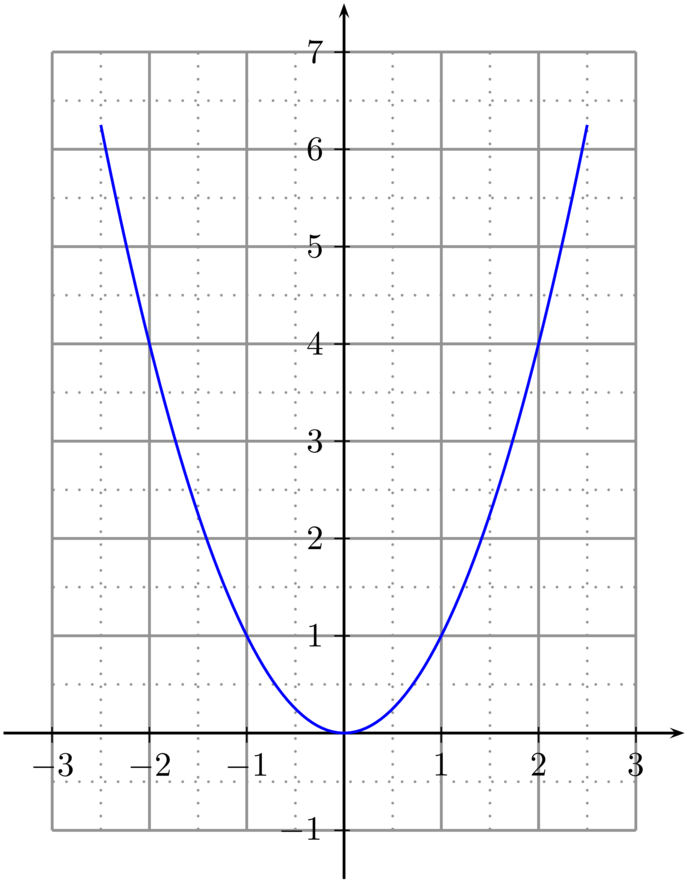
\includegraphics{Picture_FIGLabelFigFCarreQFhsWzPICTFCarreQFhsWz-for_eps.pdf}
    %\newcommand{\CaptionFigFCarreQFhsWz}{Le graphe de la fonction \( x\mapsto x^2\).}
    \input{Fig_FCarreQFhsWz.pstricks}

\end{multicols}

  \begin{example}
Compléter le tableau suivant pour la fonction $f(x)=x^2$.
\begin{equation}
\begin{array}[h]{|c|c|c|c|c|c|c|c|c|c|c|c|}
  \hline  
  x & -4 & -3 & -2 & -1 & 0 & 1 & 2 & 3 & 4 & -0,5 & 0,5  \\
  \hline
  y & 16 &&&&&&&&&&0.25\\
  \hline
\end{array}
\end{equation}
  \end{example}


\subsection{Résolution graphique d'équations}

\begin{Aretenir}
    Soit $k$, un réel fixé. Résoudre l'équation $f(x)=k$ revient à chercher les antécédents par $f$ du nombre $k$.

Le nombre de solutions de l'équation $f(x)=k$ est égal au nombre de points d'intersection de la courbe représentative de \( f\) avec la droite $d$ d'équation $y=k$. Les solutions sont les abscisses de ces points d'intersection. 
\end{Aretenir}


\begin{example}
    \begin{multicols}{2}
  Nous cherchons à résoudre $f(x)=4$. 
  \begin{itemize}
      \item 
          Nous traçons la droite horizontale d'équation \( y=4\);
      \item
          nous observons les points d'intersection de cette droite avec la courbe;
      \item
          les solutions de l'équation sont les abscisses de ces points.
  \end{itemize}

\columnbreak


%The result is on figure \ref{LabelFigExCarrexvfvre}. % From file ExCarrexvfvre
%\newcommand{\CaptionFigExCarrexvfvre}{<+Type your caption here+>}
\input{Fig_ExCarrexvfvre.pstricks}

    \end{multicols}

    Sans surprises, les solutions de \( x^2=4\) sont \( x=2\) et \( x=-2\).

\end{example}

\begin{Aretenir}
    Résoudre l'équation $f(x)=g(x)$ revient à déterminer les abscisses des points d'intersection des courbes représentatives de \( f\) et \( g\).
\end{Aretenir}


\begin{multicols}{2}

    Les solutions de l'équation \( f(x)=g(x)\) sont les abscisses des points d'intersection des deux courbes. Pour les trouver, il suffit de repérer les points d'intersections, puis de les projeter sur l'axe horizontal.

    Dans le cas de la figure ci-contre, les solutions sont approximativement \( x=-3.6\), \( x=-1.1\) et \( x=1.5\).

\columnbreak

%The result is on figure \ref{LabelFigExEquationIntersectioniSHPTw}. % From file ExEquationIntersectioniSHPTw
%\newcommand{\CaptionFigExEquationIntersectioniSHPTw}{<+Type your caption here+>}
\input{Fig_ExEquationIntersectioniSHPTw.pstricks}

\end{multicols}


\subsection{Résolution graphique d'inéquations}


%///////////////////////////////////////////////////////////////////////////////////////////////////////////////////////////
\subsubsection{Inéquation du type $f(x)<k$}
%///////////////////////////////////////////////////////////////////////////////////////////////////////////////////////////

\begin{Aretenir}
Les solutions de l'inéquation $f(x)<k$ sont les abscisses des points de $\mathscr{C}$ situés en-dessous de la droite d'équation $y=k$.

En particulier, les solutions de l'inéquation $f(x)<0$ sont les abscisses des points de la courbe représentative de \( f\) situés en-dessous de l'axe des abscisses, c'est-à-dire ayant une ordonnée strictement négative.
\end{Aretenir}

\begin{multicols}{2}
    Sur la figure ci-contre, nous résolvons \( f(x)\leq 2\). La procédure à suivre est la suivante.
    \begin{enumerate}
        \item
            Tracer la droite horizontale \( y=2\).
        \item
            Trouver les points d'intersection avec le graphe de \( f\).
        \item
            Les solutions sont les abscisses pour lesquelles le graphe de \( f\) est au-dessus du graphe de la droite \( y=2\).
    \end{enumerate}

    \columnbreak

%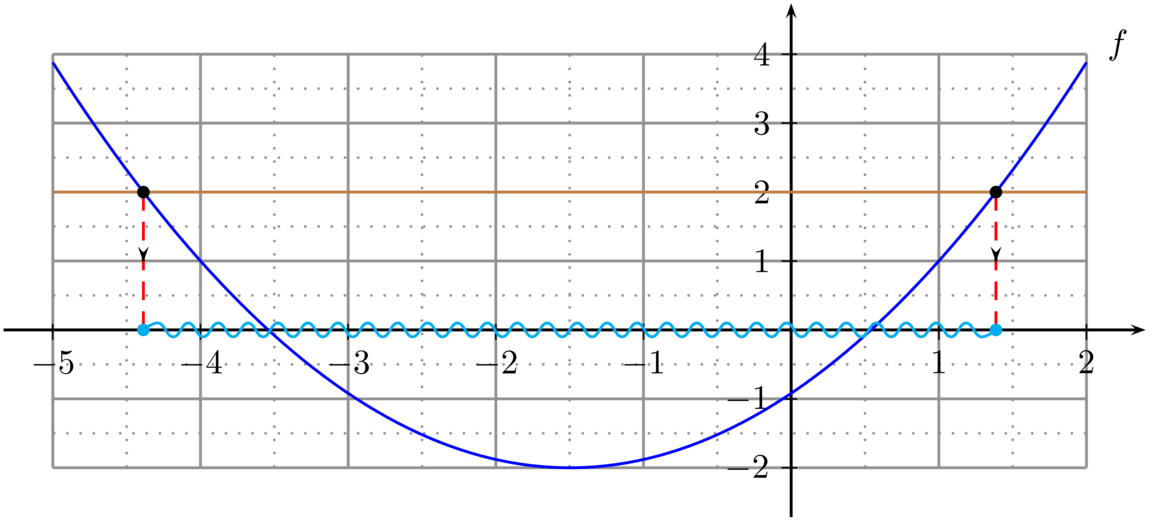
\includegraphics{Picture_FIGLabelFigExIneqOcAWMqPICTExIneqOcAWMq-for_eps.pdf}
    %\newcommand{\CaptionFigExIneqOcAWMq}{Les solutions de l'équation \( f(x)\leq 2\) sont en ondulé.}
    \input{Fig_ExIneqOcAWMq.pstricks}

\end{multicols}


\begin{remark}
    Ici nous avons résolut l'équation \( f(x)\leq 2\). Les deux points extrêmes dont partie de l'ensemble des solutions. Si nous avions résolu \( f(x)<2\), alors les points extrêmes n'auraient pas fait partie de l'ensemble des solutions.
\end{remark}

On procède de la même manière pour les inégalités du type $f(x)>k$, $f(x)\geq k$, $f(x)\leq k$. 

%///////////////////////////////////////////////////////////////////////////////////////////////////////////////////////////
\subsubsection{Inéquation du type $f(x)<g(x)$}
%///////////////////////////////////////////////////////////////////////////////////////////////////////////////////////////

Les solutions de l'inéquation $f(x)<g(x)$ sont les abscisses des points pour lesquels la courbe de \( f\) est en-dessous de la courbe de \( g\).

\newcommand{\CaptionFigExIneqfgZWStde}{En cyan, l'ensemble des solutions de l'inéquation \( f(x)<g(x)\).}
\input{Fig_ExIneqfgZWStde.pstricks}

La figure \ref{LabelFigExIneqfgZWStde} montre la résolution d'une telle inéquation. Notons que l'ensemble des solutions peut être en plusieurs morceaux.


\subsection{Tableau de variations}


Le \defe{tableau de variation}{tableau de variation} est un tableau contenant
\begin{enumerate}
    \item
        les positions des sommets,
    \item
        les flèches indiquant les endroits où la fonction est croissante ou décroissante.
\end{enumerate}
Un petit exemple valant mieux qu'un long discours\ldots

% à noter le 9 dans l'environnement suivant est le nombre de lignes sur lesquelles la figure s'étale. Je suis obligé de donner à la main parce que le tableau ne compte apparemment que pour une seule ligne. Du coup si je laisse à LaTeX le soin de calculer, les lignes de texte en-dessous de la figure (et en particulier à la page suivante si la figure est en bas de page) sont encore coupées.
\begin{wrapfigure}[9]{r}{6.0cm}     
   \vspace{-1cm}        % à adapter.
   \centering
   \input{Fig_GrapheVarREGMqx.pstricks}
\end{wrapfigure}

    Le tableau de variation de la fonction dessinée ci-contre est :
    \begin{equation*}
    \begin{array}[h]{|c|ccccccc|}
        \hline
        x&-3&&-2&&0&&2\\
        \hline
        &&&2&&&&1\\
        f(x)&&\nearrow&&\searrow&&\nearrow&\\
        &-\frac{ 9 }{2}&&&&-\frac{ 1 }{2}&&\\
        \hline
    \end{array}
    \end{equation*}
    En effet, la fonction \( f\)
    \begin{itemize}
        \item 
            part de \( x=-3\) où \( f(x)=-9/2\);
        \item
            elle monte jusqu'en \( x=-2\) où elle vaut \( f(x)=2\);
        \item
            elle descend jusqu'en \( x=0\) où elle vaut \( -\frac{ 1 }{2}\);
        \item
            elle monte jusqu'en \( x=2\) où elle vaut \( 1\).
    \end{itemize}

Le plus souvent si on donne un dessin, les nombres à placer dans un tableau de variation sont des valeur approchées à la précision du dessin. Donner les réponses en fraction n'est donc pas obligatoire. Par exemple ici au lieu d'écrire \( -9/2\) dans le tableau, il aurait été possible d'écrire \( -4.5\).

\section{Minimum et maximum}

Les notions de minima et maxima parlent, comme l'indiquent leurs noms en français, des points du graphe d'une fonction les plus hauts et les plus bas.

\begin{definition}
      Soit $f$ une fonction définie sur un intervalle $I$.
      \begin{itemize}
          \item On dit que $f$ admet le réel $m$ pour \defe{minimum}{minimum (d'une fonction)} sur $I$ si et seulement si il existe $c\in I$ tel que $f(c)=m$ et pour tout $x\in I$, $f(x)\geq m$. 
    \item On dit que $f$ admet le réel $M$ pour \defe{maximum}{maximum} sur $I$ si et seulement si il existe $d\in I$ tel que $f(d)=M$ et pour tout $x\in I$, $f(x)\leq M$.
      \end{itemize}
\end{definition}

%Sur la figure \ref{LabelFigMinMaxKNRdOd}, nous avons indiqué le minimum et le maximum de la fonction dessinée.
%\newcommand{\CaptionFigMinMaxKNRdOd}{Minimum et maximum d'une fonction.}
Sur le dessin ci-dessous nous avons indiqué le minimum et le maximum de la fonction dessinée.
\input{Fig_MinMaxKNRdOd.pstricks}

%+++++++++++++++++++++++++++++++++++++++++++++++++++++++++++++++++++++++++++++++++++++++++++++++++++++++++++++++++++++++++++ 
\section{Pour tracer}
%+++++++++++++++++++++++++++++++++++++++++++++++++++++++++++++++++++++++++++++++++++++++++++++++++++++++++++++++++++++++++++

Quelque conseils pour dessiner.
\begin{itemize}
    \item
        Pour une valeur $x$ sur l'axe des abscisses, il y a un et un seul point d'abscisse $x$ sur la courbe.
    \item
        Pour tracer une courbe, il faut placer des points. Plus on choisit de points, plus la courbe sera précise.
    \item
        Si possible, trouver quelque valeurs clefs. Par exemple on cherchera les points d'intersection entre les axes et les courbe. Le point \( (0,f(0)) \) est intéressant à mettre, ainsi que les points \( x\) tels que \( f(x)=0\).
\end{itemize}


\newcommand{\CaptionFigExFonction}{Comment tracer la fonction \( f\colon x\to 2x+1\) ?}
\input{Fig_ExFonction.pstricks}

Nous donnons à la figure \ref{LabelFigExFonction} le tracé de la fonction \( f(x)=2x+1\). La figure \ref{LabelFigExFonctionssLabelSubFigExFonction0} donne quelque points du graphe de la fonction. La figure \ref{LabelFigExFonctionssLabelSubFigExFonction1} donne le graphe complet de la fonction. Comment le construit-on ? Par définition pour chaque \( x\) sur l'axe des abscisses (il y en a une infinité), il faut calculer le nombre \( f(x)\) et mettre dans le plan le point de coordonnées \( \big( x,f(x) \big)\).

En pratique, il n'est pas possible de calculer \( f(x)\) pour \emph{tous} les \( x\) réels\footnote{Chuck Norris peut le faire.}. C'est pourquoi nous nous contentons qu'en calculer quelque uns, et nous les relions «le plus intelligemment possible».


%---------------------------------------------------------------------------------------------------------------------------
\subsection{Ce qui n'est pas une fonction}
%---------------------------------------------------------------------------------------------------------------------------

%    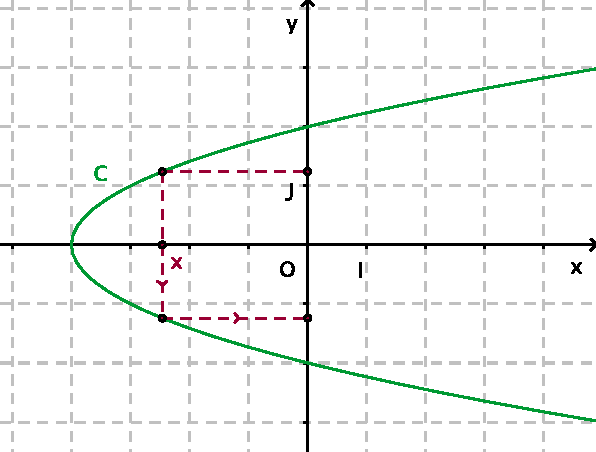
\includegraphics[width=5cm]{F_NonFct.pdf}

\begin{multicols}{2}
    Cette courbe ne représente pas une fonction, car à partir de \( x=-4\), les nombres ont deux images. Les courbes données par des fonctions sont des courbes acceptant une seule ordonnée pour chaque abscisse.

\columnbreak

%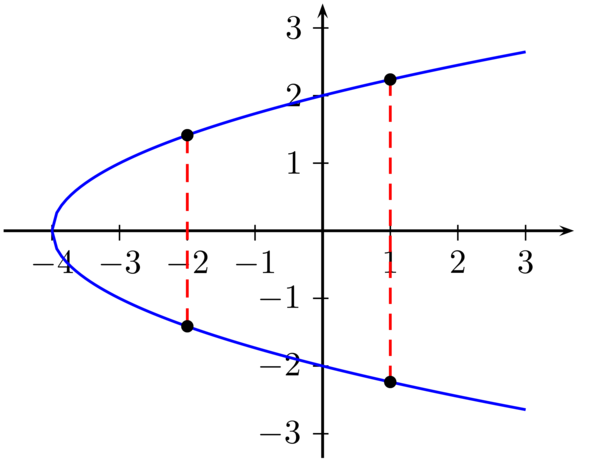
\includegraphics{Picture_FIGLabelFigPasFonctionYoQfSuPICTPasFonctionYoQfSu-for_eps.pdf}

\input{Fig_PasFonctionYoQfSu.pstricks}

\end{multicols}


Pour tracer le graphe d'une fonction affine.
\begin{itemize}
    \item
        Vu que le graphe est une droite, il suffit de deux points.
    \item
        Les fonction linéaires passent par l'origine \( (0;0)\).
    \item 
        Pour un tracé à la règle, il est plus précis de prendre deux points relativement éloignés.
    \item
        La droite \( f(x)=mx+p\) monte si \( m>0\) et descend si \( m<0\). La pente est d'autant plus forte que \( m\) est grand.
\end{itemize}

Quelque exemples à la figure \ref{LabelFigGrapheAffinHqXJGx}.
\newcommand{\CaptionFigGrapheAffinHqXJGx}{Des graphes de fonctions linéaires et affines.}
\input{Fig_GrapheAffinHqXJGx.pstricks}
      % Pour les inéquations f(x)<g(x) graphiquement, il faudra faire plus tard et il y a un truc dans 0050_resolution.tex

\chapter{Vecteurs}
% This is part of Un soupçon de mathématique sans être agressif pour autant
% Copyright (c) 2012-2014
%   Laurent Claessens
% See the file fdl-1.3.txt for copying conditions.

% Ceci sont les vecteurs sans la colinéarité sans le produit par un nombre et sans alignement de trois points.

%+++++++++++++++++++++++++++++++++++++++++++++++++++++++++++++++++++++++++++++++++++++++++++++++++++++++++++++++++++++++++++ 
\section*{Introduction}
%+++++++++++++++++++++++++++++++++++++++++++++++++++++++++++++++++++++++++++++++++++++++++++++++++++++++++++++++++++++++++++

% This is part of Un soupçon de mathématique sans être agressif pour autant
% Copyright (c) 2013
%   Laurent Claessens
% See the file fdl-1.3.txt for copying conditions.

\begin{multicols}{2}
    \begin{enumerate}
        \item
Le TER 894258 a pour horaire :
\begin{description}
    \item[14h56] Besançon-Viotte
    \item[15h06] St-Vit
    \item[15h21] Dole-Ville
    \item[15h30] Auxonne
    \item[15h39] Genlis
    \item[15h51] Dijon-Ville
\end{description}
Dessiner le trajet sur une ligne du temps en indiquant les durées entre les stations.
        \item
            En supposant les mêmes temps de parcours, quelles sont les heures d'arrivées dans les différentes gares du TER partant à 20h23 pour le même trajet ?
        \item
             Les points \( A(1;2)\), \( B(3;3)\), \( C(2;5)\) et \( D(0;4)\) forment un carré. Donner les coordonnées du «même» carré \( A'B'C'D'\) partant de \( A'(4;0)\).
         \item
             Soient les points \( K(0;0)\), \( L(4;1)\) et \( M(3;3)\). Donner les coordonnées du point \( N\) tel que \( KLMN\) soit un parallélogramme.
    \end{enumerate}
\end{multicols}


\clearpage

Éléments de réponse :
\begin{enumerate}
    \item
        Pour calculer l'intervalle de temps entre deux heures données, il faut seulement faire la différence entre les deux.
        \begin{center}
           \input{Fig_EDEYRhQ.pstricks}
        \end{center}
    \item
        Ce serait 20h23, 20h35, 20h50, 20h59,21h08,21h20. Il suffit de garder les mêmes «intervalles».
    \item
        Voici le dessin
        \begin{center}
           \input{Fig_WPrirwB.pstricks}
        \end{center}
\end{enumerate}
La conclusion est que nous pouvons faire des translations en comptant les distances «horizontales» et «verticales».

%+++++++++++++++++++++++++++++++++++++++++++++++++++++++++++++++++++++++++++++++++++++++++++++++++++++++++++++++++++++++++++
\section{Translation}
%+++++++++++++++++++++++++++++++++++++++++++++++++++++++++++++++++++++++++++++++++++++++++++++++++++++++++++++++++++++++++++

\begin{definition}  
    La \defe{translation}{translation} \( t_{\vect{ AB }}\) est la transformation du plan qui à un point \( C\) fait correspondre l'unique point \( D\) tel que les segments \( [AD]\) et \( [BC]\) aient même milieu.

Nous notons \( \vect{ AB }\) le vecteur associé à cette translation.
\end{definition}

\begin{center}
   \input{Fig_DefVecteurAXDDGP.pstricks}
\end{center}

Étant donné qu'un quadrilatère dont les diagonales se coupent en leur milieu est un parallélogramme, nous avons immédiatement le règle suivante :
\begin{Aretenir}
    Le quadrilatère \( ABDC\) est un parallélogramme si et seulement si \( D=t_{\vect{ AB }}(C)\). C'est à dire si \( D\) est donné à partir de \( C\) par la translation de vecteur \( \vect{ AB }\).

Attention : il s'agit bien de \( ABDC\) et non de \( ABCD\).
\end{Aretenir}

%Le dessin à côté de la définition \ref{DefAAJEuS}, aplati, donne immédiatement aussi
%\begin{equation}
%    t_{\vect{ AB }}(A)=B.
%\end{equation}

    Le \defe{vecteur}{vecteur} \vect{ AB } est le déplacement qui permet d'aller de $A$ à \( B\).

\begin{definition}
    Nous disons que \( \vect{ AB }=\vect{ CD }\) si et seulement si \( t_{\vect{ AB }}(C)=D\), c'est à dire si \( ABDC\) est un parallélogramme.
\end{definition}

%+++++++++++++++++++++++++++++++++++++++++++++++++++++++++++++++++++++++++++++++++++++++++++++++++++++++++++++++++++++++++++ 
\section{Somme de vecteurs}
%+++++++++++++++++++++++++++++++++++++++++++++++++++++++++++++++++++++++++++++++++++++++++++++++++++++++++++++++++++++++++++

\begin{definition}
    Le vecteur \defe{somme}{somme!de vecteur}\index{vecteur!somme} \( \vect{ AB }+\vect{ CD }\) est le vecteur qui correspond à la translation composée de \( t_{\vect{ AB }}\) par \( t_{\vect{ CD }}\)
\end{definition}

\begin{Aretenir}
    \begin{multicols}{2}
    Nous avons la \defe{relation de Chasles}{Chasles} qui permet de mettre des vecteurs «bout à bout» :
    \begin{equation}
        \vect{ AB }+\vect{ BC }=\vect{ AC }.
    \end{equation}

    \columnbreak

%Une illustration de la relation de Chasles est donnée à la figure \ref{LabelFigChaslesGTRtKR}. % From file ChaslesGTRtKR
%\newcommand{\CaptionFigChaslesGTRtKR}{La somme $ \vect{ AB }+\vect{ BC }$ est le vecteur $ \vect{ AC }$.}
\input{Fig_ChaslesGTRtKR.pstricks}

    \end{multicols}
\end{Aretenir}

%+++++++++++++++++++++++++++++++++++++++++++++++++++++++++++++++++++++++++++++++++++++++++++++++++++++++++++++++++++++++++++ 
\section{Coordonnées d'un vecteur dans un repère}
%+++++++++++++++++++++++++++++++++++++++++++++++++++++++++++++++++++++++++++++++++++++++++++++++++++++++++++++++++++++++++++

\begin{multicols}{2}
    \begin{definition}
        Les coordonnées du vecteur \( \vect{ u }\) dans un repère d'origine \( O\) sont les coordonnées du point \( M\) tel que \( \vect{ u }=\vect{ OM }\).
    \end{definition}

    \columnbreak

    %The result is on figure \ref{LabelFigfigureNNgEEzx}. % From file figureNNgEEzx
    %\newcommand{\CaptionFigfigureNNgEEzx}{<+Type your caption here+>}
    \begin{center}
\input{Fig_figureNNgEEzx.pstricks}
    \end{center}
\end{multicols}
Dans le cas ci-dessus, nous avons \( \vect{ AB }=\vect{ OM }\) et les coordonnées de \( M\) sont \( M=(-2;1)\). Nous notons
\begin{equation}
    \vect{ AB }=\begin{pmatrix}
        -2    \\ 
        1    
    \end{pmatrix}.
\end{equation}

\begin{Aretenir}
    \begin{multicols}{2}
    Si \( A=(x_A;x_B)\) et \( B=(x_B;y_B)\) alors
    \begin{equation*}
        \vect{ AB }=\begin{pmatrix}
            x_B-x_A    \\ 
            y_B-y_A    
        \end{pmatrix}.
    \end{equation*}

    \columnbreak

   %The result is on figure \ref{LabelFigfigureLEOvqez}. % From file figureLEOvqez
%\newcommand{\CaptionFigfigureLEOvqez}{<+Type your caption here+>}
    \begin{center}
\input{Fig_figureLEOvqez.pstricks}
    \end{center}

    \end{multicols}
   % TODO : lire le TODO qu'il y a dans le fichier phystricksfigureLEOvqez 
\end{Aretenir}

\begin{Aretenir}
    \begin{enumerate}
        \item
    Le vecteur \( \vect{ AB }\) est \defe{nul}{vecteur!nul} si les points \( A\) et \( B\) sont confondus. On le note alors \( \vect{ 0 }\).

        \item
    Nous définissons aussi \( -\vect{ AB }=\vect{ BA }\).
    \end{enumerate}
    
\end{Aretenir}
%--------------------------------------------------------------------------------------------------------------------------- 
\section{Somme et coordonnées}
%---------------------------------------------------------------------------------------------------------------------------

\begin{propriete}
    Si dans un repère \( \vect{ u }=\begin{pmatrix}
        x    \\ 
        y    
    \end{pmatrix}\) et \( \vect{ v }=\begin{pmatrix}
        x'    \\ 
        y'    
    \end{pmatrix}\), alors 
    \begin{equation}
        \vect{ u }+\vect{ v }=\begin{pmatrix}
            x+x'    \\ 
            y+y'    
        \end{pmatrix}.
    \end{equation}
    
\end{propriete}

\begin{proof}
    Soient \( A\) et \( B\) des points tels que \( \vect{ u }=\vect{ AB }\). Vu que les vecteurs peuvent être placés n'importe où, nous pouvons placer \( \vect{ v }\) au point \( B\) et dire \( \vect{ v }=\vect{ BC }\) pour un certain point \( C\). Par les relations de Chasles,
    \begin{equation}    \label{EqASjyYXs}
        \vect{ u }+\vect{ v }=\vect{ AC }=\begin{pmatrix}
            x_C-x_A    \\ 
            y_C-y_A    
        \end{pmatrix}.
    \end{equation}
    
    D'autre part étant donné que \( \vect{ u= }\vect{ AB }\), nous avons
    \begin{subequations}
        \begin{align}
            x=x_B-x_A\\
            y=y_B-y_A;
        \end{align}
    \end{subequations}
    et vu que \( \vect{ v }=\vect{ BC }\)
    \begin{subequations}
        \begin{align}
            x'=x_C-x_B\\
            y'=y_C-y_B
        \end{align}
    \end{subequations}
    Du coup nous avons
    \begin{subequations}
        \begin{align}
            x+x'=(x_B-x_A)+(x_C-x_B)=x_C-x_A\\
            y+y'=(y_B-y_A)+(y_C-y_B)=y_C-y_A
        \end{align}
    \end{subequations}
    En comparant avec \eqref{EqASjyYXs}, nous avons bien
    \begin{equation}
        \vect{ u }+\vect{ v }=\vect{ AC }=\begin{pmatrix}
            x_C-x_A    \\ 
            y_C-y_A    
        \end{pmatrix}=\begin{pmatrix}
            x+x'    \\ 
            y+y'    
        \end{pmatrix},
    \end{equation}
    ce qu'il fallait démontrer.
\end{proof}


\chapter{Intervalle de fluctuation et de intervalle confiance}
% This is part of Un soupçon de mathématique sans être agressif pour autant
% Copyright (c) 2013
%   Laurent Claessens
% See the file fdl-1.3.txt for copying conditions.

% Ce fichier est celui pour les secondes.


\setcounter{section}{-1}
%+++++++++++++++++++++++++++++++++++++++++++++++++++++++++++++++++++++++++++++++++++++++++++++++++++++++++++++++++++++++++++ 
\section{Comptons des petites boules}
%+++++++++++++++++++++++++++++++++++++++++++++++++++++++++++++++++++++++++++++++++++++++++++++++++++++++++++++++++++++++++++

% This is part of Un soupçon de mathématique sans être agressif pour autant
% Copyright (c) 2013
%   Laurent Claessens
% See the file fdl-1.3.txt for copying conditions.

La classe est divisée en groupes, chacun contenant des perles turquoises et des perles blanches. Les sacs sont identiques mais inconnus. Le but de l'activité est de déterminer ce contenu sans compter toutes les perles. Voici le protocole :
\begin{itemize}
    \item Tirer une perle au hasard dans le sac,
    \item Noter sa couleur.
    \item La remettre dans le sac.
\end{itemize}
Nous parlons de tirage \defe{avec remise}{avec remise!tirage}.

%--------------------------------------------------------------------------------------------------------------------------- 
\subsection*{Après 10 tirages}
%---------------------------------------------------------------------------------------------------------------------------

Reporter les résultats de vos tirages en notant T ou B dans le tableau suivant :

\begin{tabular}[]{|c|c|c|c|c|c|c|c|c|}
    \hline
    &&&&&&&&\\
    \hline
\end{tabular}

Ce tirage forme un \defe{échantillon}{échantillon} du contenu du sac.
\begin{enumerate}
    \item
        Quelle est la fréquence d'apparition de la couleur turquoise ?
     \item
        Reporter les fréquences des autres groupes :
        \begin{tabular}[]{|c|c|c|c|c|c|c|c|c|c|}
        \hline
        &&&&&&&&\\
        \hline
    \end{tabular}
\item
    Que constate-t-on ?
\end{enumerate}

%--------------------------------------------------------------------------------------------------------------------------- 
\subsection*{Après 50 tirages}
%---------------------------------------------------------------------------------------------------------------------------

Effectuer encore \( 40\) tirages.
\begin{enumerate}
    \item
        Calculer la fréquence d'apparition de la couleur turquoise.
    \item
        Compléter le tableau de fréquences d'apparition du turquoise suivant :
        \begin{equation*}
            \begin{array}[]{|c|c|c|c|}
                \hline
                &\text{échantillon de taille 10}&\text{échantillon de taille 40}&\text{Échantillon de taille 50}\\
                  \hline
                  \text{Fréq.}&&&\\ 
                  \hline 
                   \end{array}
               \end{equation*}
               
\end{enumerate}

%--------------------------------------------------------------------------------------------------------------------------- 
\subsection*{Après 100 tirages}
%---------------------------------------------------------------------------------------------------------------------------

Effectuer \( 50\) nouveaux tirages et reporter les résultats :

\begin{equation*}
    \begin{array}[]{|c|c|c|c|}
      \hline
        &\text{Taille 10}&\text{Taille 50}&\text{Taille 100}\\
       \hline
       \text{Fréq.}&&&\\ 
       \hline 
  \end{array}
\end{equation*}
               
Écrire les résultats des autres groupes :
        \begin{tabular}[]{|c|c|c|c|c|c|c|c|c|c|}
        \hline
        &&&&&&&&\\
        \hline
    \end{tabular}

Combien de tirages ont été faits en tout dans la classe ? Quelle est la fréquence observée des boules turquoises ?


%+++++++++++++++++++++++++++++++++++++++++++++++++++++++++++++++++++++++++++++++++++++++++++++++++++++++++++++++++++++++++++ 
\section{Intervalle de confiance}
%+++++++++++++++++++++++++++++++++++++++++++++++++++++++++++++++++++++++++++++++++++++++++++++++++++++++++++++++++++++++++++

Nous avons vu que plus la taille de l'échantillon était grande, plus la fréquence estimée était précise. Précisons le mode opératoire pour fixer le vocabulaire :
\begin{Aretenir}
    Nous avons une \defe{population}{population} de perles à étudier. La \defe{proportion}{proportion} des perles turquoises est inconnue, mais en extrayant un \defe{échantillon}{échantillon} nous pouvons calculer une \defe{fréquence}{fréquence} qui sera une approximation de la proportion.
\end{Aretenir}

Le résultat suivant donne une version précise de la phrase «Plus l'échantillon est grand, plus l'approximation est bonne».
\begin{Aretenir}
    Nous mesurons la fréquence \( f\) d'apparition d'un caractère dans un échantillon de taille \( n\) issu d'une population dont la proportion (inconnue) d'apparition du caractère est \( p\). Alors il y a \( 95\%\) de chances que 
    \begin{equation}
        p\in \mathopen[ f-\frac{1}{ \sqrt{n} } , f+\frac{1}{ \sqrt{n} } \mathclose].
    \end{equation}
    Cet intervalle est l'\defe{intervalle de confiance}{intervalle!de confiance} de \( p\) au seuil \( 95\%\).
\end{Aretenir}

\begin{example}
Lors d’une élection, un sondage portant sur un échantillon aléatoire de $1000$ personnes donne $400$ votants en faveur d’un candidat \( L\). Au risque d’erreur de 5\%, quelle information peut-on obtenir sur la proportion réelle d’électeurs envisageant de voter pour $L$ ?    

La fréquence du vote pour le candidat \( L\) dans l'échantillon est de \( f=0.4\), et la taille de l'échantillon est \( n=400\). Donc il y a une probabilité \( 0.95\) que la proportion réelle de votants pour \( L\) soit dans
\begin{equation}
    \mathopen[ f-\frac{1}{ \sqrt{n} } , f+\frac{1}{ \sqrt{n} } \mathclose]=\mathopen[ 0.4-0.05 , 0.5+0.05 \mathclose]=\mathopen[ 0.35 , 0.55 \mathclose].
\end{equation}
Ce que dit ce résultat est que il devrait y avoir entre \( 35\%\) et \( 55\%\) de votants pour le candidat \( L\).

Autrement dit, si le résultat de l'élection donne moins de \( 35\%\) ou plus de \( 55\%\) au candidat \( L\), nous pouvons dire qu'il n'y a que \( 5\%\) de chances que le résultat soit dû au hasard. Il y a une probabilité \( 0.95\) que soit le sondage avait été mal fait, soit qu'un événement imprévu ait changé des votes au dernier moment.

\end{example}

%+++++++++++++++++++++++++++++++++++++++++++++++++++++++++++++++++++++++++++++++++++++++++++++++++++++++++++++++++++++++++++ 
\section{Intervalle de fluctuation}
%+++++++++++++++++++++++++++++++++++++++++++++++++++++++++++++++++++++++++++++++++++++++++++++++++++++++++++++++++++++++++++

Nous nous intéressons maintenant à un problème un peu différent.

Nous avons une population dont nous étudions un caractère pour lequel nous croyons déjà savoir la fréquence. Nous voulons confirmer l'idée en analysant un échantillon.

\begin{example}
    Un charlatan(?) prétend avoir le pouvoir lire à travers des cartes. Pour vérifier ses dires, on construit un jeu de cartes de façon à ce que chaque carte représente soit un rond, soit un carré soit un triangle.

    On lui présente une centaine de ces cartes successivement, face cachée et on lui demande si elle représente un rond, un carré ou un triangle.

    Si, comme le pensent certains sceptiques, la personne se contente de répondre au hasard alors il devrait répondre correctement environ \( 33\) fois sur la centaine d'essais (une fois sur trois). Nous observons \( 37\) réussites. Est-ce qu'on peut dire que la personne a un réel pouvoir ?

\end{example}

Nous ne savons pas quelle est la proportion réelle de réussite de la personne, mais sa fréquence de réussite est de \( 0.37\) sur \( 100\) essais. Donc au seuil de \( 95\%\) nous pouvons dire que sa proportion de réussite est comprise dans
\begin{equation}
    \mathopen[ 0.37-\frac{1}{ \sqrt{100} } ;0.37+\frac{1}{ \sqrt{100} } \mathclose]=\mathopen[ 0.27 ;0.47 \mathclose].
\end{equation}
Ce résultat est très compatible avec la proportion de réussite attendue en cas de réponse au hasard (parce que \( 0.33\) est dans l'intervalle).

Le résultat-clef est le suivant.
\begin{Aretenir}
    Soit une population dans laquelle une proportion \( p\) d'individus présentent une certaine caractéristique. Soit aussi un échantillon de taille \( n\) prélevé au hasard dans cette population. Nous notons \( f\) la fréquence des individus de l'échantillon présentant la caractéristique. 

    Si \( p\) est entre \( 0.2\) et \( 0.8\) et si \( n\geq 30\), alors il y a \( 95\%\) de chances que 
    \begin{equation}
        f\in\mathopen[ p-\frac{1}{ \sqrt{n} } ; p+\frac{1}{ \sqrt{n} } \mathclose].
    \end{equation}
    Cet intervalle est appelé \defe{intervalle de fluctuation}{intervalle!de fluctuation} de l'échantillon.
\end{Aretenir}

Cet intervalle peut être justifié à partir de l'autre :
\begin{equation}
\xymatrix{%
    &   p\in\mathopen[ f-\frac{1}{ \sqrt{n}} , f+\frac{1}{ \sqrt{n} } \mathclose]\ar[rd]\ar[ld] &  \\
    p\geq f-\frac{1}{ \sqrt{n}}\ar[d]&&p\leq f+\frac{1}{ \sqrt{n}}  \ar[d]\\
    f\leq p+\frac{1}{ \sqrt{n}}\ar[rd] && p-\frac{1}{ \sqrt{n}}\leq f\ar[ld]\\
    & f\in\mathopen[ p-\frac{1}{ \sqrt{n} } , p+\frac{1}{ \sqrt{n}} \mathclose]  &
   }
\end{equation}


\begin{example}
    Si \( 25\%\) de la population a des yeux bleus et qu'on pêche \( 500\) personnes au hasard, il y a environ \( 95\%\) de chances que parmi ces \( 500\) la proportion d'yeux bleus sera comprise dans l'intervalle
    \begin{equation}
        \mathopen[ 0.25-\frac{1}{ \sqrt{500} } ; 0.25+\frac{1}{ \sqrt{500} } \mathclose]\simeq\mathopen[ 0.25-0.045 ; 0.25+0.045 \mathclose]=\mathopen[ 0.205 ; 0.294 \mathclose].
    \end{equation}
    En termes de nombre de personnes, cela signifie qu'on aura entre \( 102\) et \( 148\) personnes à yeux bleus parmi les \( 500\) personnes tirées au hasard.

    Il n'y a que \( 2.5\%\) de chance d'obtenir moins de \( 102\) personnes à yeux bleus sur \( 500\), et environ \( 2.5\%\) de chances d'en avoir plus de \( 148\).

    Donc si on tire un échantillon de \( 500\) personnes et qu'on y voit $170$ avec des yeux bleus, on peut se dire trois choses :
    \begin{itemize}
        \item Le sondage a été mal fait, on n'a pas bien tiré les personnes au hasard, on a mal compté, \ldots
        \item Dans la population, en fait il n'y a pas vraiment \( 25\%\) de personnes aux yeux bleus, mais plus.
        \item On a été victime du hasard, et en réalité il n'y a aucune faute; on avait moins de deux chances et demi sur \( 100\) que ça arrive, mais c'est toujours possible.
    \end{itemize}
    Notons que \( 5\) fois sur \( 100\), un sondage donnera une proportion non conforme à ce à quoi on s'attend. Cela fait environ une fois sur \( 20\).
\end{example}


\chapter{Équations de droites}
% This is part of Un soupçon de mathématique sans être agressif pour autant
% Copyright (c) 2012-2014
%   Laurent Claessens
% See the file fdl-1.3.txt for copying conditions.


Ce chapitre parle d'équations de droites et se voit après le chapitre sur les fonctions affines.
\begin{enumerate}
    \item
        Droite passant par des points donnés.
    \item 
        Parallélisme, intersection.
    \item
        Proportionnalité, coefficient directeur.
    \item
        Lien avec la colinéarité des vecteurs.
    \item
        Dire si trois points sont alignés.
\end{enumerate}

%+++++++++++++++++++++++++++++++++++++++++++++++++++++++++++++++++++++++++++++++++++++++++++++++++++++++++++++++++++++++++++ 
\section*{Introduction}
%+++++++++++++++++++++++++++++++++++++++++++++++++++++++++++++++++++++++++++++++++++++++++++++++++++++++++++++++++++++++++++

% This is part of Un soupçon de mathématique sans être agressif pour autant
% Copyright (c) 2014
%   Laurent Claessens
% See the file fdl-1.3.txt for copying conditions.

Soit le programme suivant :

\begin{fmpage}{0.9\linewidth}

    Demander \( x\) et \( y\).

    Si \( y=-2x\) alors :

    \hspace{1cm} Écrire «oui» 

    Sinon :

    \hspace{1cm} Écrire «non» 

\end{fmpage}

Donner quelque valeurs de \( x\) et \( y\) pour lesquelles le programme écrit «oui» ? À quoi sert ce programme ?

Mêmes questions pour ce programme :

\begin{fmpage}{0.9\linewidth}

    Demander \( x\) et \( y\).

    Si \( x=4\) alors :

    \hspace{1cm} Écrire «oui» 

    Sinon :

    \hspace{1cm} Écrire «non» 

\end{fmpage}


%+++++++++++++++++++++++++++++++++++++++++++++++++++++++++++++++++++++++++++++++++++++++++++++++++++++++++++++++++++++++++++ 
\section{Équation de droite}
%+++++++++++++++++++++++++++++++++++++++++++++++++++++++++++++++++++++++++++++++++++++++++++++++++++++++++++++++++++++++++++

\begin{theorem}
    Toute droite du plan a une équation.
    \begin{enumerate}
        \item
            Si \( d\) est une droite parallèle à l'axe des ordonnées alors elle a une équation \( d:x=c\) pour un certain réel \( c\).
        \item
            Si \( d\) est une droite non parallèle à l'axe des ordonnées, alors elle a une équation \( y=mx+p\) pour certains réels \( m\) et \( p\).
    \end{enumerate}
\end{theorem}

\begin{proof}
    \begin{enumerate}
        \item
            Soit une droite \( d\) parallèle à l'axe des ordonnées. Elle coupe l'axe des abscisses en un point \( C\) de coordonnées \( (c,0)\). Par définition du système de coordonnée, tout point de \( d\) a alors une abscisse égale à \( c\).
        \item
            Nous supposons à présent que la droite \( d\) n'est pas parallèle à l'axe des ordonnées. Cette droite coupe l'axe vertical en un point \( P\) de coordonnées \( (0;p)\) et l'axe \( x=1\) au point \( Q(1;q)\).
            \begin{center}
   \input{Fig_OKeZlpK.pstricks}
            \end{center}
            Le théorème de Thalès nous indique que
            \begin{equation}
                \frac{ MS }{ PS }=\frac{ QR }{ PR },
            \end{equation}
            c'est à dire
            \begin{equation}
                \frac{ y_M-p }{ x_M }=\frac{ q-p }{ 1 },
            \end{equation}
            c'est à dire
            \begin{equation}
                y_M=(q-p)x_M+p.
            \end{equation}
            En posant \( m=q-p\) nous avons bien l'équation demandée :
            \begin{equation}
                y=mx+p.
            \end{equation}
    \end{enumerate}
\end{proof}

\begin{theorem}
    Soit la fonction affine \( f(x)=mx+p\). Alors pour tout nombres distincts \( u\) et \( v\) nous avons
    \begin{equation}
        \frac{ f(u)-f(v) }{ u-v }=m.
    \end{equation}
\end{theorem}

\begin{proof}
    Soient \( u\) et \( v\), deux réels distincts. Nous calculons
    \begin{equation}
        f(u)-f(v)=mu+p-(mv+p)=mu-mv=m(u-v).
    \end{equation}
    En divisant par \( u-v\) on trouve le résultat annoncé.
\end{proof}

%+++++++++++++++++++++++++++++++++++++++++++++++++++++++++++++++++++++++++++++++++++++++++++++++++++++++++++++++++++++++++++ 
\section{Déterminer une équation de droite}
%+++++++++++++++++++++++++++++++++++++++++++++++++++++++++++++++++++++++++++++++++++++++++++++++++++++++++++++++++++++++++++

%TODO : Décommenter cette démonstration.
%
%Soient les points \( A(x_A;y_A)\) et \( B(x_B;y_B)\). Nous voulons déterminer l'équation de la droite
%\begin{equation}
%    y=mx+p
%\end{equation}
%qui passe par ces deux points. Vu que \( A\) est sur cette droite, ses coordonnées vérifient l'équation :
%\begin{equation}
%    y_A=mx_A+p
%\end{equation}
%et pour la même raison :
%\begin{equation}
%    y_B=mx_B+p
%\end{equation}
%En soustrayant ces deux équations :
%\begin{equation}
%    y_A-y_B=  mx_A+p-(mx_B+p)=m(x_A-x_B),
%\end{equation}
%ou encore
%\begin{equation}
%    y_A-y_B=m(x_A-x_B), 
%\end{equation}
%c'est à dire
%\begin{equation}
%    m=\frac{ y_A-y_B }{ x_A-x_B }.
%\end{equation}
%
\begin{Aretenir}
    Le coefficient directeur d'une droite passant par deux points \( A(x_A;y_A)\) et \( B(x_B;y_B)\) est donné par la formule
    \begin{equation}
        m=\frac{ y_B-y_A }{ x_B-x_A }.
    \end{equation}
    L'ordonnée à l'origine se calcule en posant \( y_A=mx_A+p\) et en résolvant pour \( p\).
\end{Aretenir}

\begin{example}
    Trouver l'équation de la droite passant par \( A(-1;-2)\) et \( B(1;4)\).

    D'abord
    \begin{equation}
        m=\frac{ 4-(-2) }{ 1-(-2) }=\frac{ 6 }{ 3 }=3.
    \end{equation}
    Nous cherchons donc une équation du type \( y=3x+p\). Il s'agit donc de trouver \( p\) pour avoir \emph{en même temps}
    \begin{equation}
            -2=3\times (-1)+p
    \end{equation}
    et
    \begin{equation}
        4=3\times 1+p
    \end{equation}
    La solution est \( p=1\). Au final l'équation cherchée est
    \begin{equation}
        y=3x+1.
    \end{equation}
    
\end{example}


%+++++++++++++++++++++++++++++++++++++++++++++++++++++++++++++++++++++++++++++++++++++++++++++++++++++++++++++++++++++++++++ 
\section{Intersection de droites}
%+++++++++++++++++++++++++++++++++++++++++++++++++++++++++++++++++++++++++++++++++++++++++++++++++++++++++++++++++++++++++++

Nous avons déjà vu que les fonctions affines \( f(x)=mx+p\) et \( g(x)=m'x+p'\) ont des droites représentatives parallèles si et seulement si \( m=m'\).

\begin{Aretenir}
    Trouver l'abscisse du point d'intersection des droites \( y=mx+p\) et \( y=m'x+p\) revient à résoudre l'équation
    \begin{equation}
        mx+p=m'x+p.
    \end{equation}
    Pour trouver l'ordonnée il suffit de mettre la réponse dans l'équation d'une des deux droites.

    ATTENTION : si \( m=m'\), les droites sont parallèles et il n'y a pas d'intersection.
\end{Aretenir}

\begin{example}
    Trouver le point d'intersection des droites \( d_1:y=2x-4\) et \( d_2:y=-x+5\). Ce sont les droites représentatives des fonctions affines \( f(x)=2x+4\) et \( g(x)=-x+5\). L'abscisse du point d'intersection est donnée par l'équation \( f(x)=g(x)\), c'est à dire
    \begin{equation}
        2x-4=-x+5,
    \end{equation}
    dont la solution est \( x=3\). 

    Pour trouver l'ordonnée du point d'intersection il faut calculer \( f(3)\) ou \( g(3)\), qui doivent donner le même résultat.
    \begin{equation}
        f(3)=g(3)=2.
    \end{equation}
    Dont le point d'intersection est le point
    \begin{equation}
        I=(3;2).
    \end{equation}
\end{example}

%+++++++++++++++++++++++++++++++++++++++++++++++++++++++++++++++++++++++++++++++++++++++++++++++++++++++++++++++++++++++++++ 
\section{Colinéarité}
%+++++++++++++++++++++++++++++++++++++++++++++++++++++++++++++++++++++++++++++++++++++++++++++++++++++++++++++++++++++++++++

\begin{wrapfigure}{r}{10.cm}
   \vspace{-0.5cm}        % à adapter.
   \centering
   \input{Fig_RVZNtGK.pstricks}
\end{wrapfigure}


Le théorème de Thalès nous donne une bonne façon de savoir si trois points sont alignés. Les points \( A\), \( B\) et \( C\) sont alignés si et seulement si
\begin{equation}
    \frac{ y_C-y_A }{ x_C-x_A }=\frac{ y_B-y_A }{ x_B-x_A }.
\end{equation}
C'est à dire si et seulement si les coefficients directeurs des droites \( (AB)\) et \( (AC)\) sont les mêmes.


\chapter{Vecteurs : colinéarité}
% This is part of Un soupçon de mathématique sans être agressif pour autant
% Copyright (c) 2012-2013
%   Laurent Claessens
% See the file fdl-1.3.txt for copying conditions.


%+++++++++++++++++++++++++++++++++++++++++++++++++++++++++++++++++++++++++++++++++++++++++++++++++++++++++++++++++++++++++++ 
\section{Parallélisme et colinéarité}
%+++++++++++++++++++++++++++++++++++++++++++++++++++++++++++++++++++++++++++++++++++++++++++++++++++++++++++++++++++++++++++

\begin{definition}
    Deux vecteurs \( \vect{ u }\) et \( \vect{ v }\) sont \defe{colinéaires}{colinéaire (vecteurs)} si il existe \( \lambda\in \eR\) tel que \( \vect{ u }=\lambda\vect{ v }\).
\end{definition}

\begin{propriete}
    \begin{enumerate}
        \item
            Les droites \( (AB)\) et \( (CD)\) sont parallèles si et seulement si les vecteurs \( \vect{ AB }\) et \( \vect{ CD }\) sont colinéaires.
        \item
            Les points \( A\), \( B\) et \( C\) sont alignés si et seulement si les vecteurs \( \vect{ AB }\) et \( \vect{ AC }\) sont colinéaires.
    \end{enumerate}
\end{propriete}

Nous savons qu'un quadrilatère ayant deux côtés parallèles de même longueur est un parallélogramme. Donc nous avons le critère suivant pour savoir si \( ABCD\) est un parallélogramme :
\begin{equation}
    \vect{ AB }=\vect{ CD }.
\end{equation}
Bien entendu les autres côtés fonctionnent aussi :
\begin{equation}
    \vect{ AC }=\vect{ BD }.
\end{equation}
Si une de ces deux égalités vectorielle est satisfaite, alors \( ABCD\) est un parallélogramme.

\begin{example}
    Les points \( A=(-2;-3)\), \( B=(-1,-1)\), \( C=(2;-2)\) et \( D=(1;-4)\) forment un parallélogramme.
\end{example}

%--------------------------------------------------------------------------------------------------------------------------- 
\subsection{Le milieu revisité}
%---------------------------------------------------------------------------------------------------------------------------

Notre travail sur les coordonnées de vecteurs nous permet de donner une preuve alternative à la propriété \ref{PropFHznUfJ}.

\begin{propriete}
    Soient les points \( A\), \( B\) et \( K\) tels que \( K\) soit le milieu du segment \( [AB]\). Alors nous avons \( \vect{ AK }=\vect{ BK }\).
\end{propriete}

\begin{proof}
    Nous divisons la preuve en petits pas.
    \begin{subproof}
        \item[Création du repère]
            Nous considérons un repère orthonormé \footnote{En réalité il n'est pas obligatoire qu'il soit orthonormé, mais ça ne coûte rien qu'il le soit.} dont \( A\) est l'origine.
        \item[Coordonnées des points]
            Dans le repère choisi, nous considérons les coordonnées des points \( K=(x_K;y_K)\) et \( B=(x_B,y_B)\). Nous allons aussi nommer \( I\) et \( J\) les points \( I=(x_K;0)\) et \( J=(x_B;0)\). Le dessin est maintenant comme suit :

            \begin{center}
%The result is on figure \ref{LabelFigfigureSZyxsvp}. % From file figureSZyxsvp
%\newcommand{\CaptionFigfigureSZyxsvp}{<+Type your caption here+>}
\input{Fig_figureSZyxsvp.pstricks}
            \end{center}
        \item[Utilisation du théorème de Thalès]
            Vu que les droites \( (KI)\) et \( (BJ)\) sont parallèles, nous pouvons utiliser le théorème de Thalès :
            \begin{equation}
                \frac{ AB }{ AK }=\frac{ AJ }{ AI }=\frac{ BJ }{ KI }.
            \end{equation}
            Nous remplaçons dans ces égalités les longueurs par ce qu'on connait. Vu que \( K\) est le milieu de \( [AB] \), nous avons \( \frac{ AB }{ AK }=2\). D'autre part, $AJ=x_B$, \( AI=x_K\), \( BJ=y_B\) et \( KI=y_K\), donc
            \begin{equation}
                2=\frac{ x_B }{ x_K }
            \end{equation}
            et
            \begin{equation}
                2=\frac{ y_B }{ y_K }.
            \end{equation}
            Autrement dit,
            \begin{equation}
                x_B=2x_K
            \end{equation}
            et
            \begin{equation}
                y_B=2y_K.
            \end{equation}
        \item[Les vecteurs en présence]
            Les vecteurs \( \vect{ AB }\) et \( \vect{ AK }\) ont pour coordonnées
            \begin{subequations}
                \begin{align}
                    \vect{ AB }=\begin{pmatrix}
                        x_B    \\ 
                        y_B    
                    \end{pmatrix}\\
                    \vect{ AK }=\begin{pmatrix}
                        x_K    \\ 
                        y_K    
                    \end{pmatrix},
                \end{align}
            \end{subequations}
            Donc, étant donné que \( x_B=2x_K\) et \( y_B=2y_K\) nous avons
            \begin{equation}    \label{EqNGxKxaY}
                \vect{ AB }=2\vect{ AK }.
            \end{equation}
        \item[Utilisation de la loi de Chasles et conclusion]
            Nous savons que \( \vect{ AB }=\vect{ AK }+\vect{ KB }\), donc en replaçant \( \vect{ AB }\) par \( 2\vect{ AK }\) nous avons
            \begin{equation}
                2\vect{ AK }=\vect{ AK }+\vect{ KB },
            \end{equation}
            ce qui implique que
            \begin{equation}
                \vect{ AK }=\vect{ KB },
            \end{equation}
            ce qu'il fallait.
    \end{subproof}
\end{proof}
Nous notons aussi au passage l'intéressante formule \eqref{EqNGxKxaY} :
\begin{equation}
    \vect{ AB }=2\vect{ AK }.
\end{equation}



\chapter{Les fonctions du second degré}
%This is part of Un soupçon de mathématique sans être agressif pour autant
% Copyright (c) 2012-2014
%   Laurent Claessens
% See the file fdl-1.3.txt for copying conditions.

%+++++++++++++++++++++++++++++++++++++++++++++++++++++++++++++++++++++++++++++++++++++++++++++++++++++++++++++++++++++++++++ 
\section*{Activité}
%+++++++++++++++++++++++++++++++++++++++++++++++++++++++++++++++++++++++++++++++++++++++++++++++++++++++++++++++++++++++++++

%This is part of Un soupçon de mathématique sans être agressif pour autant
% Copyright (c) 2014
%   Laurent Claessens
% See the file fdl-1.3.txt for copying conditions.

Bertrand l'artisan vend des pots de terre cuite sur le marché. Chaque pot lui coûte \( 2\)€ de matériel. Au début de sa carrière il avait fixé le prix à \( 10\)€ et il vendait \( 8\) pots par semaine. Chaque semaine Bertrand baisse son prix de \( 0.5\)€ et vend alors \( 4\) pots supplémentaires.

\begin{enumerate}
    \item
        Donner le nombre de pots vendus ainsi que son bénéfice au début de sa carrière ainsi qu'après \( 1\), \( 2\) et \( 3\) semaines.
    \item
        Exprimer le nombre de pots vendus ainsi que le bénéfice après \( x\) semaines.
    \item
        Tracer un graphique.
    \item
        Après combien de baisses de prix Bertrand aura-t-il intérêt à cesser de baisser le prix ?
\end{enumerate}


%+++++++++++++++++++++++++++++++++++++++++++++++++++++++++++++++++++++++++++++++++++++++++++++++++++++++++++++++++++++++++++ 
\section{Paraboles}
%+++++++++++++++++++++++++++++++++++++++++++++++++++++++++++++++++++++++++++++++++++++++++++++++++++++++++++++++++++++++++++

\begin{definition}
    Une fonction \defe{polynôme du second degré}{polynôme!second degré} est une fonction définie sur \( \eR\) de la forme
    \begin{equation}
        f(x)=ax^2+bx+c
    \end{equation}
    avec \( a\neq 0\). Le graphe d'un polynôme du second degré est une \defe{paraboles}{parabole}. 

    Ce graphe sera noté \( y=ax_0+bx+c\).
\end{definition}

\newcommand{\CaptionFigLSaSLoS}{Quelque paraboles.}
\input{Fig_LSaSLoS.pstricks}


%--------------------------------------------------------------------------------------------------------------------------- 
%\subsection{Axe de symétrie}
%---------------------------------------------------------------------------------------------------------------------------

%L'axe de symétrie de la courbe représentative de \( f(x)=ax^2+bx+c\) se trouve en résolvant par rapport à \( s\) l'équation
%\begin{equation}
%    f(s+h)=f(s-h).
%\end{equation}

\begin{Aretenir}
    La parabole \( y=ax^2+bx+x\) est tournée vers le haut si \( a>0\) et tournée vers le bas si \( a<0\).

    Le sommet de la parabole \( y-ax^2+bx+c\) se trouve à l'abscisse \( x_0=-\frac{ b }{ 2a }\) et la droite verticale \( x=-\frac{ -b }{ 2a }\) est un axe de symétrie de la parabole.
\end{Aretenir}
Quelque unes sont dessinées à la figure \ref{LabelFigLSaSLoS}. % From file LSaSLoS

\clearpage

%+++++++++++++++++++++++++++++++++++++++++++++++++++++++++++++++++++++++++++++++++++++++++++++++++++++++++++++++++++++++++++ 
\section{Tableau de variation}
%+++++++++++++++++++++++++++++++++++++++++++++++++++++++++++++++++++++++++++++++++++++++++++++++++++++++++++++++++++++++++++

Les tableaux de variations sont
\begin{multicols}{2}

    \begin{center}
        Si \( a>0\)

        \begin{equation*}
            \begin{array}[]{c|ccccc}
                x&&&-\frac{ b }{ 2a }&&\\
                \hline
                &\infty&&&&\infty\\
                f(x)&&\searrow&&\nearrow&\\
                &&&f\left( -\frac{ b }{ 2a } \right)&&\\
            \end{array}
        \end{equation*}
        
    \end{center}

    \columnbreak

    \begin{center}
        Si \( a<0\)


        \begin{equation*}
            \begin{array}[]{c|ccccc}
                x&&&-\frac{ b }{ 2a }&&\\
                \hline
                &&&f\left( -\frac{ b }{ 2a } \right)&&\\
                f(x)&&\nearrow&&\searrow&\\
                &-\infty&&&&-\infty\\
            \end{array}
        \end{equation*}
    \end{center}
\end{multicols}

%+++++++++++++++++++++++++++++++++++++++++++++++++++++++++++++++++++++++++++++++++++++++++++++++++++++++++++++++++++++++++++ 
\section{La fonction carré}
%+++++++++++++++++++++++++++++++++++++++++++++++++++++++++++++++++++++++++++++++++++++++++++++++++++++++++++++++++++++++++++

La fonction carré est la fonction définie sur \( \eR\) qui à \( x\) fait correspondre \( x^2\).

\begin{multicols}{2}

        \begin{equation*}
            \begin{array}[]{c|ccccc}
                x&-\infty&&0&&+\infty\\
                \hline
                &+\infty&&&&+\infty\\
                &&\searrow&&\nearrow&\\
                &&&0&&
            \end{array}
        \end{equation*}

        \columnbreak

        %The result is on figure \ref{LabelFigfigureXNAufCh}. % From file figureXNAufCh
        %\newcommand{\CaptionFigfigureXNAufCh}{<+Type your caption here+>}
        \begin{center}
\input{Fig_figureXNAufCh.pstricks}
        \end{center}
\end{multicols}

% Plus besoin de ça parce que la parabole en générale est vue avant la fonction carré.
%\begin{definition}
%    Le graphe de la fonction carré est une \defe{parabole}{parabole}.
%\end{definition}

%+++++++++++++++++++++++++++++++++++++++++++++++++++++++++++++++++++++++++++++++++++++++++++++++++++++++++++++++++++++++++++ 
\section{Double antécédent et solutions d'équations}
%+++++++++++++++++++++++++++++++++++++++++++++++++++++++++++++++++++++++++++++++++++++++++++++++++++++++++++++++++++++++++++

\begin{Aretenir}
    La fonction carré a pour principale caractéristique d'avoir \emph{deux} antécédents pour chaque image (à part pour zéro). Les antécédents du nombre \( a\) sont \( \sqrt{a}\) et \( -\sqrt{a}\).
\end{Aretenir}

\begin{example}
    Les carrés de \( 4\) et de \( -4\) sont tous les deux \( 16\).
\end{example}

Au niveau des inéquations, cela se ressent. La fonction \( x^2\) sera par exemple plus petite que \( 4\) non seulement pour les \( x\in\mathopen[ 0 , 3 \mathclose]\) mais aussi pour \( x\in\mathopen[ -3 , 0 \mathclose]\).

Nous voyons cela sur la figure \ref{LabelFigfigureEWDVDTS} qui montre les solution de \( f(x)\leq 4\). % From file figureEWDVDTS
\newcommand{\CaptionFigfigureEWDVDTS}{La résulution graphique d'une inéquation avec la fonction carré.}
\input{Fig_figureEWDVDTS.pstricks}

%+++++++++++++++++++++++++++++++++++++++++++++++++++++++++++++++++++++++++++++++++++++++++++++++++++++++++++++++++++++++++++ 
\section{Encadrement}
%+++++++++++++++++++++++++++++++++++++++++++++++++++++++++++++++++++++++++++++++++++++++++++++++++++++++++++++++++++++++++++

\begin{Aretenir}
    La fonction carré est décroissante sur \( \mathopen] -\infty , 0 \mathclose]\) et croissante sur \( \mathopen[ 0 , \infty [\).
    \begin{enumerate}
        \item
            Si \( 0<x<y\), alors \( 0<x^2<y^2\).
        \item
            Si \( x<y<0\), alors \( x^2>y^2>0\).
    \end{enumerate}
\end{Aretenir}


%This is part of Un soupçon de mathématique sans être agressif pour autant
% Copyright (c) 2012-2014
%   Laurent Claessens
% See the file fdl-1.3.txt for copying conditions.


% Ce fichier contient le second degré pour les secondes; pas pour les premières.

%+++++++++++++++++++++++++++++++++++++++++++++++++++++++++++++++++++++++++++++++++++++++++++++++++++++++++++++++++++++++++++ 
\section{Paraboles}
%+++++++++++++++++++++++++++++++++++++++++++++++++++++++++++++++++++++++++++++++++++++++++++++++++++++++++++++++++++++++++++

\begin{definition}
    Une fonction \defe{polynôme du second degré}{polynôme!second degré} est une fonction de la forme
    \begin{equation}
        f(x)=ax^2+bx+c
    \end{equation}
    avec \( a\neq 0\). L'ensemble de définition des polynômes est \( \eR\). Le graphe d'un polynôme du second degré est une \defe{paraboles}{parabole}. 
\end{definition}

\newcommand{\CaptionFigLSaSLoS}{Quelque paraboles.}
\input{Fig_LSaSLoS.pstricks}

Les paraboles ont toutes la même forme générale : une courbe tournée vers le haut ou vers le bas. La courbe de \( f(x)=ax^2+bx+x\) est tournée vers le haut si \( a>0\) et tournée vers le bas si \( a<0\).
Quelque unes sont dessinées à la figure \ref{LabelFigLSaSLoS}. % From file LSaSLoS

%--------------------------------------------------------------------------------------------------------------------------- 
%\subsection{Axe de symétrie}
%---------------------------------------------------------------------------------------------------------------------------

%L'axe de symétrie de la courbe représentative de \( f(x)=ax^2+bx+c\) se trouve en résolvant par rapport à \( s\) l'équation
%\begin{equation}
%    f(s+h)=f(s-h).
%\end{equation}

\begin{Aretenir}
    Le sommet de la parabole \( ax^2+bx+c\) se trouve à l'abscisse \( x_0=-\frac{ b }{ 2a }\) et la droite verticale est un axe de symétrie de la parabole.
\end{Aretenir}

%--------------------------------------------------------------------------------------------------------------------------- 
\subsection{Tableau de variation}
%---------------------------------------------------------------------------------------------------------------------------

Les tableaux de variations sont
\begin{multicols}{2}

    \begin{center}
        Si \( a>0\)

        \begin{equation*}
            \begin{array}[]{c|ccccc}
                x&&&-\frac{ b }{ 2a }&&\\
                \hline
                &\infty&&&&\infty\\
                f(x)&&\searrow&&\nearrow&\\
                &&&f\left( -\frac{ b }{ 2a } \right)&&\\
            \end{array}
        \end{equation*}
        
    \end{center}

    \columnbreak

    \begin{center}
        Si \( a<0\)


        \begin{equation*}
            \begin{array}[]{c|ccccc}
                x&&&-\frac{ b }{ 2a }&&\\
                \hline
                &&&f\left( -\frac{ b }{ 2a } \right)&&\\
                f(x)&&\nearrow&&\searrow&\\
                &-\infty&&&&-\infty\\
            \end{array}
        \end{equation*}
    \end{center}
\end{multicols}


\chapter{Les feuilles toutes faites}
% FEUILLE POUR ALLER EN SALLE INFORMATIQUE.
\begin{feuilleExo}{Pour aller en salle info}
    \begin{multicols}{2}
    \Exo{smath-0539}
    \Exo{smath-0540}
    \Exo{smath-0589}
    \Exo{smath-0583}
    \Exo{smath-0581}
    \Exo{smath-0580}
    \Exo{smath-0582}
    \Exo{smath-0579}
    \end{multicols}
\end{feuilleExo}

%FEUILLE D'ALGORITHMIQUE
\begin{multicols}{2}
    \Exo{smath-0526}    % algo
    \Exo{smath-0555}    % algo
    \Exo{smath-0578}    % algo, DS des autres
    \Exo{smath-0551}    % algo De DS des autres
    \Exo{smath-0577}
    \Exo{smath-0528}    %algo
    \Exo{smath-0527}    %algo
\end{multicols}

%FEUILLE DE SECOURS NUMÉRO 1, FÉVRIER 2014
\begin{feuilleExo}{Feuille de secours de math numéro 1}
    \begin{multicols}{2}
        \Exo{smath-0637}
        \Exo{smath-0638}
\Exo{smath-0639}
\Exo{smath-0640}
\Exo{smath-0643}
\Exo{smath-0641}
\Exo{smath-0642}
\Exo{smath-0644}
\Exo{smath-0645}
\Exo{smath-0646}
\Exo{smath-0647}
    \end{multicols}
\end{feuilleExo}


%FEUILLE DE SECOURS NUMÉRO 2, MARS 2014
\begin{feuilleExo}{Feuille de secours de math numéro 2}
    \begin{multicols}{2}
        \Exo{smath-0648}
\Exo{smath-0678}
\Exo{smath-0679}
\Exo{smath-0677}
\Exo{smath-0680}
\Exo{smath-0682}
\Exo{smath-0683}
\Exo{smath-0684}
\Exo{smath-0685}
    \end{multicols}
\end{feuilleExo}

% FEUILLE D'AP pour les 1ES
\begin{feuilleExo}{Feuille d'AP première ES}
\Exo{smath-0557}
\Exo{smath-0559}
\Exo{Premiere-0006}
\Exo{smath-0558}
\Exo{smath-0399}
\end{feuilleExo}

% FEUILLE D'AP pour les 2DE -- logique
\begin{feuilleExo}{Feuille d'AP de seconde, logique}
\Exo{smath-0560}
\Exo{smath-0561}
\Exo{smath-0562}
\Exo{smath-0563}
\Exo{smath-0564}    % document d'accompagnement de fonctions.
\Exo{smath-0433}
\Exo{smath-0471}
\end{feuilleExo}

% LES EXOS POUR CEUX QUI ONT TERMINÉ
\begin{feuilleExo}{Des questions plus compliquées}
\Exo{smath-0541}
\Exo{smath-0545}
\Exo{smath-0543}
\Exo{smath-0544}
\Exo{smath-0542}
\end{feuilleExo}



% ----------------- À partir d'ici c'est sans doute le bordel.

\chapter{Autres choses sur les fonctions}
%This is part of Un soupçon de mathématique sans être agressif pour autant
% Copyright (c) 2012-2013
%   Laurent Claessens, Pauline Klein
% See the file fdl-1.3.txt for copying conditions.

\begin{example}
    Soit la fonction \( f(x)=3x-1\).
    \begin{enumerate}
        \item
            Le point \( (0;-1)\) est sur la courbe représentative de \( f\) parce que \( f(0)=1\).
        \item
            Le point \( (10;29)\) est également sur la courbe parce que \( f(10)=29\).
        \item
            Le point \( (2;3)\) n'est par contre pas sur le graphe parce que \( f(2)=5\neq 4\).
    \end{enumerate}
\end{example}

%+++++++++++++++++++++++++++++++++++++++++++++++++++++++++++++++++++++++++++++++++++++++++++++++++++++++++++++++++++++++++++
\section{Petit tour de magie}
%+++++++++++++++++++++++++++++++++++++++++++++++++++++++++++++++++++++++++++++++++++++++++++++++++++++++++++++++++++++++++++

\begin{Aprojeter}
    \begin{example} \label{ExemVmCkIH}
        Un petit tour de magie. Choisissez un nombre entre \( 1\) et \( 10\). Ajoutez \( 5\), multipliez par \( 2\), ajoutez \( 7\), enlevez le double du nombre de départ.
    \end{example}
\end{Aprojeter}

\begin{Aprojeter}
    Pouvez-vous trouver un petit tour de magie qui commence par
    \begin{itemize}
        \item Multiplier par \( 3\)
        \item Faire \( +2\)
        \item \ldots
    \end{itemize}
    et qui donne toujours \( 5\) ?
\end{Aprojeter}

\begin{Aprojeter}
    \lstinputlisting{ex_algo18.py}
\end{Aprojeter}


%+++++++++++++++++++++++++++++++++++++++++++++++++++++++++++++++++++++++++++++++++++++++++++++++++++++++++++++++++++++++++++ 
\section{Ensemble de définition}
%+++++++++++++++++++++++++++++++++++++++++++++++++++++++++++++++++++++++++++++++++++++++++++++++++++++++++++++++++++++++++++

\begin{definition}
    Soit \( \defD\) un ensemble de nombres. On définit une \defe{fonction}{fonction} \( f\) sur \( \defD\) en associant à chaque nombre \( x\) dans \( \defD\) un seul nombre \( y\). Dans ce cas nous disons que \( f\) est une fonction de la \defe{variable}{variable} \( x\).
\end{definition}

\begin{example}
    Soit la fonction qui à la longueur d'un segment fait correspondre la surface du carré construit sur ce segment. Cette fonction n'est définie que sur les nombres positifs (parce qu'il n'existe pas de segments de longueurs négatives). Nous écrivons donc
    \begin{equation}
        \begin{aligned}
            f\colon \mathopen[ 0 , \infty [&\to \eR \\
            x&\mapsto x^2,
        \end{aligned}
    \end{equation}
    et nous avons \( f(x)=x^2\).

    Le symbole \( \mathopen[ 0 , \infty [\) représente l'ensemble de tous les nombres de \( 0\) (y compris) à l'infini, c'est à dire tous les nombres plus grands ou égaux à \( 0\).
\end{example}

\begin{example}
    Soit la fonction qui a un nombre entier fait correspondre la somme de ses chiffres. Par exemple \( f(0)=0\) et \( f(123)=6\). Cette fonction est définie sur les entiers et retourne un entier. Nous pouvons écrire
    \begin{equation}
        \begin{aligned}
            f\colon \eN&\to \eN \\
            x&\mapsto f(x). 
        \end{aligned}
    \end{equation}
    Ici il est compliqué de donner une forme explicite pour \( f\).
\end{example}

\begin{example}
    La fonction carré est :
    \begin{equation}
        \begin{aligned}
            f\colon \eR&\to \eR \\
            x&\mapsto x^2 
        \end{aligned}
    \end{equation}
    Notons que c'est presque la même que la fonction «surface du carré». La différence est le contexte.
\end{example}

\begin{example}
    La fonction racine carré est :
    \begin{equation}
        \begin{aligned}
            \sqrt{}\colon \mathopen[ 0 , \infty [&\to \eR  \\
                x&\mapsto \sqrt{x}. 
        \end{aligned}
    \end{equation}
\end{example}

\begin{example}
    La fonction inverse est :
    \begin{equation}
        \begin{aligned}
            f\colon \eR\setminus\{ 0 \}&\to \eR \\
            x&\mapsto \frac{1}{ x }. 
        \end{aligned}
    \end{equation}
    La notation \( \eR\setminus\{ 0 \}\) représente l'ensemble de tous les nombres sauf zéro.
\end{example}

%--------------------------------------------------------------------------------------------------------------------------- 
\subsection{Intermède : pourquoi ne pas diviser par zéro ?}
%---------------------------------------------------------------------------------------------------------------------------

La fraction \( \frac{1}{ 0.1 }\) est le nombre de fois que \( 0.1\) rentre dans \( 1\). Cela vaut \( 10\) parce qu'il faut \( 10\) soit \( 0.1\) pour faire \( 1\).

Que vaut \( \frac{1}{ 0.0001 }\) ? C'est le nombre de fois que \( 0.0001\) rentre dans \( 1\), c'est à dire dix mille.

Que vaudrait \( \frac{1}{ 0 }\) ? C'est le nombre de fois qu'il faut prendre zéro pour obtenir \( 1\).

\begin{example}
    Considérons la fonction qui a un nombre fait correspondre son inverse : \( f\colon x\mapsto \frac{1}{ x }\). Pour se dérouiller le cerveau, je propose quelque valeurs :
    \begin{equation}
        \begin{aligned}[]
            f(1)&=1&f(5)&=\frac{1}{ 5 }&f(\frac{ 2 }{ 3 })=\frac{ 3 }{ 2 }\\
            f(\frac{ 1 }{ 4 })&=4&f(-3)&=-\frac{1}{ 3 }&f(-1)&=-1.
        \end{aligned}
    \end{equation}
    Cette fonction est implémentée en python de la façon suivante :

\lstinputlisting{ex_inverse.py}

donne

%\lstinputlisting[title=Résultat]{res_ex_inverse.txt}
\VerbatimInput{res_ex_inverse.txt}

Très clairement, python ne veut pas calculer l'inverse de zéro et plante sur un message on ne peut plus clair : \info{ZeroDivisionError: division by zero}.

Effectivement, l'inverse de zéro n'existe pas. L'ensemble de définition de notre fonction \( f(x)=1/x\) n'est donc pas \( \eR\) tout entier, mais seulement \( \eR\setminus\{ 0 \}\).

\end{example}

\begin{Aretenir}        \label{ArtJgipNt}
    Il n'est pas permis de diviser par zéro. Une fonction qui contient un dénominateur ne peut pas avoir dans son ensemble de définition des \( x\) qui annulent le dénominateur. Autrement dit dès que vous voyez
    \begin{equation}
        \frac{1}{ f(x) }
    \end{equation}
    vous devez résoudre l'équation \( f(x)=0\).
\end{Aretenir}

%+++++++++++++++++++++++++++++++++++++++++++++++++++++++++++++++++++++++++++++++++++++++++++++++++++++++++++++++++++++++++++
\section{Antécédent}
%+++++++++++++++++++++++++++++++++++++++++++++++++++++++++++++++++++++++++++++++++++++++++++++++++++++++++++++++++++++++++++

\begin{Aretenir}
Une fonction associe à chaque nombre de l'ensemble de définition \emph{un seul} nombre, appelé \defe{image}{image}. Si \( a\) est un nombre, un \defe{antécédent}{antécédent} de \( a\) par la fonction \( f\) est un nombre \( x\in\defD\) tel que 
\begin{equation}
    f(x)=a.
\end{equation}
Autrement dit, les antécédents de \( a\) sont les éléments de \( \eR\) dont l'image par \( f\) est \( a\).

Il peut arriver qu'un nombre ait plusieurs antécédents.
\end{Aretenir}


\begin{example}
    Pour la fonction \( f(x)=2x-1\), un antécédent de \( 5\) est le nombre \( 3\). Un antécédent du nombre \( -10\) est la nombre \( -9/2\).
\end{example}

\begin{Aretenir}
    Trouver les antécédents de \( a\) par la fonction \( f\) revient à trouver les solutions de l'équation
    \begin{equation}
        f(x)=a.
    \end{equation}
\end{Aretenir}


\begin{example}

    Les antécédents de \( 4\) pour la fonction \( f(x)=2x-1\) sont les solutions de l'équation
    \begin{equation}
        2x-1=4
    \end{equation}
    c'est à dire \( x=\frac{ 5 }{2}\). Il se fait qu'il y en a un seul.

    Plus généralement l'antécédent de \( a\) pour cette fonction est la solution de l'équation
    \begin{equation}
        2x-1=a,
    \end{equation}
    c'est à dire le nombre \( x=\frac{ a+1 }{ 2 }\).
\end{example}

\begin{example} \label{EqlaIGDz}
    Si nous avons une série statistique de \( n\) valeurs, pour trouver le premier quartile nous devons diviser \( n\) par \( 4\) et prendre l'entier le plus proche vers le haut. Cela donne le numéro de la valeur correspondante au premier quartile.

    En python, la fonction qui donne le numéro de la valeur du premier quartile en fonction de \( n\) est
    \begin{quote}
        \info{math.ceil(n/4)}
    \end{quote}
    Notons \( f\) cette fonction. Son ensemble de définition est l'ensemble des entiers non nuls. Le graphique de cette fonction est donné à la figure \ref{LabelFigMathCeilwCXIJZ}.
\newcommand{\CaptionFigMathCeilwCXIJZ}{Le numéro de la valeur du premier quartile en fonction du nombre de valeurs.}
\input{Fig_MathCeilwCXIJZ.pstricks}

    Le graphique est uniquement constitué de points. Pas de lignes entre, parce qu'il n'existe pas de séries statistiques comprenant \( 3.7\) valeurs par exemple. 
\end{example}

\Exo{Seconde-0053}

\begin{example}
    Soit la fonction définie sur \( \defD=\{ -5,-1,1,3,9 \}\) de la façon suivante :
    \begin{equation}
        \begin{array}[h]{|c||c|c|c|c|c|c|}
            \hline
            x&-5&-1&1&3&9&10\\
            \hline
            f(x)&0&2&-3&7&2&5\\
            \hline
        \end{array}
    \end{equation}
    Nous pouvons dire que
    \begin{enumerate}
        \item
            L'image de \( 1\) par \( f\) est \( -3\).
        \item
            L'unique antécédent de \( 7\) est \( 3\).
        \item
            Les nombres \( -1\) et \( 9\) sont tous deux des antécédents de \( 2\).
    \end{enumerate}
\end{example}

\begin{example}
    Soit la fonction \( f(x)=(x+1)^2\). Nous avons \( f(-1)=0\), \( f(4)=25\); nous disons que \( 0\) est l'image de \( -1\) par \( f\) et que \( 25\) est l'image de \( 4\) par \( f\).

    Remarquons que \( f(-2)=1\) et \( f(0)=1\). Donc \( -2\) et \( 0\) sont deux antécédents de \( 1\).
\end{example}

\begin{example}
    Le nombre \( 4\) est un antécédent de \( 3\) pour la fonction \( f(x)=\frac{ x }{ 2 }+1\).
\end{example}

\begin{example}
    Les nombres \( 3\) et \( -3\) sont tout deux des antécédents de \( 9\) pour la fonction \( x\mapsto x^2\).
\end{example}

%+++++++++++++++++++++++++++++++++++++++++++++++++++++++++++++++++++++++++++++++++++++++++++++++++++++++++++++++++++++++++++
\section{Modélisation par une fonction}
%+++++++++++++++++++++++++++++++++++++++++++++++++++++++++++++++++++++++++++++++++++++++++++++++++++++++++++++++++++++++++++

Les exemples de fonctions dans la «vraie» vie sont nombreux.

\begin{example}
    Soit un triangle rectangle isocèle dont les côtés de l'angle droit sont de longueur \( x\). Alors la surface est donnée par la fonction
    \begin{equation}
        f(x)=\frac{ x^2 }{2}.
    \end{equation}
    L'ensemble de définition est \( \defD=\mathopen] 0 , \infty \mathclose[\) parce que \( x\) représente une longueur.
\end{example}

\begin{example}
    Un vélo se déplace à \( \unit{20}{\kilo\meter\per\hour}\). Après un temps \( t\), il aura parcouru une distance
    \begin{equation}
        d(t)=20t
    \end{equation}
    kilomètres. Ici l'ensemble de définition est plus délicat; il dépend du contexte.

    Notons que la variable d'une fonction n'est pas obligatoirement toujours notée \( x\) et que la fonction n'est pas toujours obligatoirement notée \( f\).
\end{example}

\begin{example}
    Vous verrez dans un cours de physique que si on lance un objet verticalement avec une vitesse initiale \( v_0\), alors la hauteur en fonction du temps est donnée par
    \begin{equation}
        h(t)=v_0t-\frac{ gt^2 }{2}
    \end{equation}
    où \( g\) est l'accélération de la gravitation sur Terre (environ \( \unit{10}{\meter\per\second\squared}\)).
\end{example}


%---------------------------------------------------------------------------------------------------------------------------
\section{Résolution graphique d'(in)équations} 
%---------------------------------------------------------------------------------------------------------------------------

\subsection{Lecture graphique des images et des antécédents}

\begin{multicols}{2}

    Nous considérons la fonction
    \begin{equation}
        \begin{aligned}
            f\colon \eR&\to \eR \\
            x&\mapsto x^2 
        \end{aligned}
    \end{equation}
    dont le graphe est donné ci-contre. À chaque réel $x$, nous associons l'abscisse $y=f(x)$.  À l'aide du graphe donné, répondre aux questions suivantes.

    \begin{itemize}
        \item Image de $1,5$ ? 
        \item Antécédent de $3,5$ ?  
        \item Antécédent de $-1$ ? 
        \item Antécédent de $0$ ? 
    \end{itemize}

    \columnbreak

    %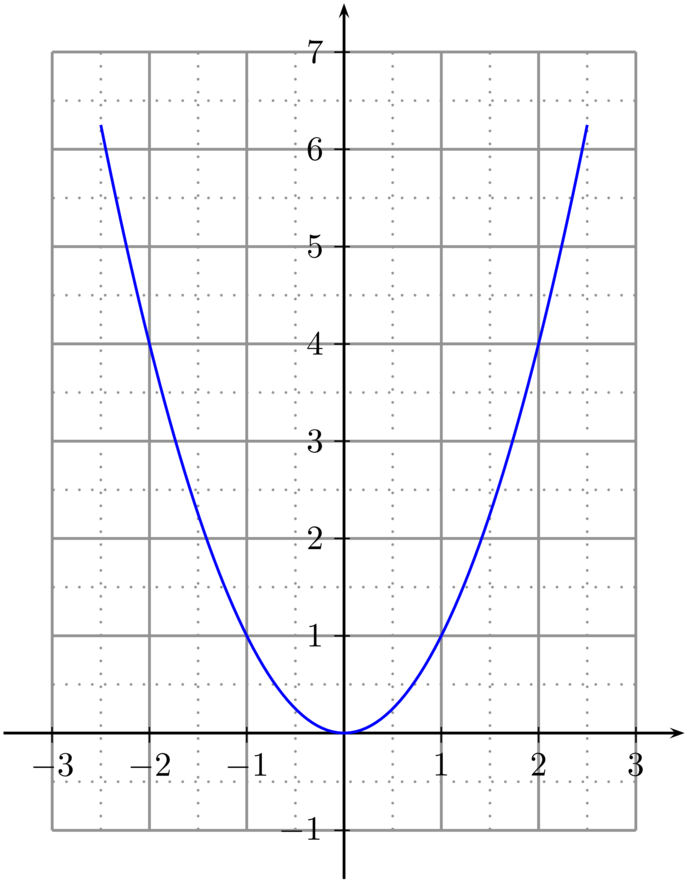
\includegraphics{Picture_FIGLabelFigFCarreQFhsWzPICTFCarreQFhsWz-for_eps.pdf}
    %\newcommand{\CaptionFigFCarreQFhsWz}{Le graphe de la fonction \( x\mapsto x^2\).}
    \input{Fig_FCarreQFhsWz.pstricks}

\end{multicols}

  \begin{example}
Compléter le tableau suivant pour la fonction $f(x)=x^2$.
\begin{equation}
\begin{array}[h]{|c|c|c|c|c|c|c|c|c|c|c|c|}
  \hline  
  x & -4 & -3 & -2 & -1 & 0 & 1 & 2 & 3 & 4 & -0,5 & 0,5  \\
  \hline
  y & 16 &&&&&&&&&&0.25\\
  \hline
\end{array}
\end{equation}
  \end{example}


\subsection{Résolution graphique d'équations}

\begin{Aretenir}
    Soit $k$, un réel fixé. Résoudre l'équation $f(x)=k$ revient à chercher les antécédents par $f$ du nombre $k$.

Le nombre de solutions de l'équation $f(x)=k$ est égal au nombre de points d'intersection de la courbe représentative de \( f\) avec la droite $d$ d'équation $y=k$. Les solutions sont les abscisses de ces points d'intersection. 
\end{Aretenir}


\begin{example}
    \begin{multicols}{2}
  Nous cherchons à résoudre $f(x)=4$. 
  \begin{itemize}
      \item 
          Nous traçons la droite horizontale d'équation \( y=4\);
      \item
          nous observons les points d'intersection de cette droite avec la courbe;
      \item
          les solutions de l'équation sont les abscisses de ces points.
  \end{itemize}

\columnbreak


%The result is on figure \ref{LabelFigExCarrexvfvre}. % From file ExCarrexvfvre
%\newcommand{\CaptionFigExCarrexvfvre}{<+Type your caption here+>}
\input{Fig_ExCarrexvfvre.pstricks}

    \end{multicols}

    Sans surprises, les solutions de \( x^2=4\) sont \( x=2\) et \( x=-2\).

\end{example}

\begin{Aretenir}
    Résoudre l'équation $f(x)=g(x)$ revient à déterminer les abscisses des points d'intersection des courbes représentatives de \( f\) et \( g\).
\end{Aretenir}


\begin{multicols}{2}

    Les solutions de l'équation \( f(x)=g(x)\) sont les abscisses des points d'intersection des deux courbes. Pour les trouver, il suffit de repérer les points d'intersections, puis de les projeter sur l'axe horizontal.

    Dans le cas de la figure ci-contre, les solutions sont approximativement \( x=-3.6\), \( x=-1.1\) et \( x=1.5\).

\columnbreak

%The result is on figure \ref{LabelFigExEquationIntersectioniSHPTw}. % From file ExEquationIntersectioniSHPTw
%\newcommand{\CaptionFigExEquationIntersectioniSHPTw}{<+Type your caption here+>}
\input{Fig_ExEquationIntersectioniSHPTw.pstricks}

\end{multicols}


\subsection{Résolution graphique d'inéquations}


%///////////////////////////////////////////////////////////////////////////////////////////////////////////////////////////
\subsubsection{Inéquation du type $f(x)<k$}
%///////////////////////////////////////////////////////////////////////////////////////////////////////////////////////////

\begin{Aretenir}
Les solutions de l'inéquation $f(x)<k$ sont les abscisses des points de $\mathscr{C}$ situés en-dessous de la droite d'équation $y=k$.

En particulier, les solutions de l'inéquation $f(x)<0$ sont les abscisses des points de la courbe représentative de \( f\) situés en-dessous de l'axe des abscisses, c'est-à-dire ayant une ordonnée strictement négative.
\end{Aretenir}

\begin{multicols}{2}
    Sur la figure ci-contre, nous résolvons \( f(x)\leq 2\). La procédure à suivre est la suivante.
    \begin{enumerate}
        \item
            Tracer la droite horizontale \( y=2\).
        \item
            Trouver les points d'intersection avec le graphe de \( f\).
        \item
            Les solutions sont les abscisses pour lesquelles le graphe de \( f\) est au-dessus du graphe de la droite \( y=2\).
    \end{enumerate}

    \columnbreak

%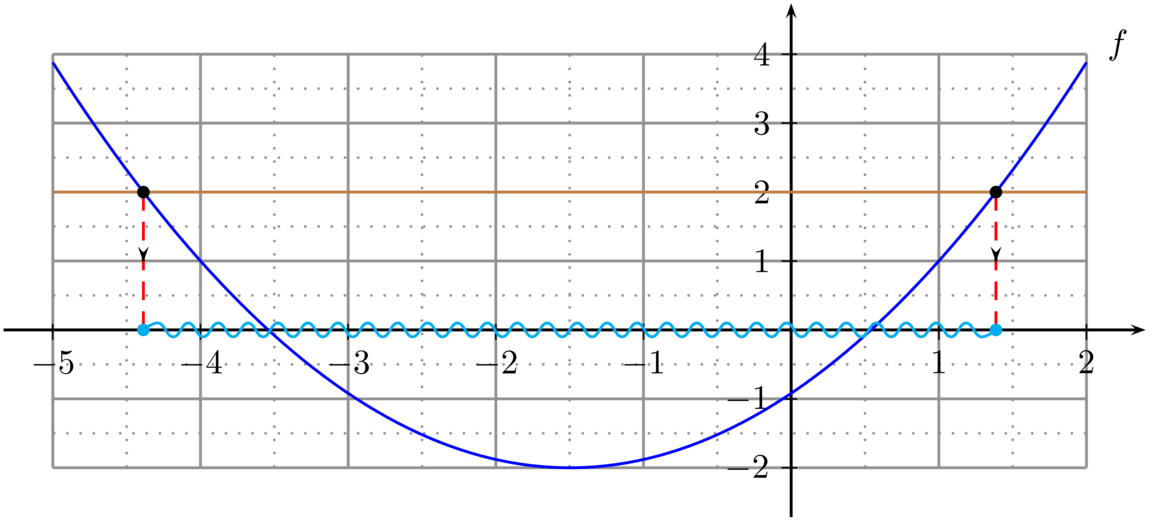
\includegraphics{Picture_FIGLabelFigExIneqOcAWMqPICTExIneqOcAWMq-for_eps.pdf}
    %\newcommand{\CaptionFigExIneqOcAWMq}{Les solutions de l'équation \( f(x)\leq 2\) sont en ondulé.}
    \input{Fig_ExIneqOcAWMq.pstricks}

\end{multicols}


\begin{remark}
    Ici nous avons résolut l'équation \( f(x)\leq 2\). Les deux points extrêmes dont partie de l'ensemble des solutions. Si nous avions résolu \( f(x)<2\), alors les points extrêmes n'auraient pas fait partie de l'ensemble des solutions.
\end{remark}

On procède de la même manière pour les inégalités du type $f(x)>k$, $f(x)\geq k$, $f(x)\leq k$. 

%///////////////////////////////////////////////////////////////////////////////////////////////////////////////////////////
\subsubsection{Inéquation du type $f(x)<g(x)$}
%///////////////////////////////////////////////////////////////////////////////////////////////////////////////////////////

Les solutions de l'inéquation $f(x)<g(x)$ sont les abscisses des points pour lesquels la courbe de \( f\) est en-dessous de la courbe de \( g\).

\newcommand{\CaptionFigExIneqfgZWStde}{En cyan, l'ensemble des solutions de l'inéquation \( f(x)<g(x)\).}
\input{Fig_ExIneqfgZWStde.pstricks}

La figure \ref{LabelFigExIneqfgZWStde} montre la résolution d'une telle inéquation. Notons que l'ensemble des solutions peut être en plusieurs morceaux.


\subsection{Tableau de variations}


Le \defe{tableau de variation}{tableau de variation} est un tableau contenant
\begin{enumerate}
    \item
        les positions des sommets,
    \item
        les flèches indiquant les endroits où la fonction est croissante ou décroissante.
\end{enumerate}
Un petit exemple valant mieux qu'un long discours\ldots

% à noter le 9 dans l'environnement suivant est le nombre de lignes sur lesquelles la figure s'étale. Je suis obligé de donner à la main parce que le tableau ne compte apparemment que pour une seule ligne. Du coup si je laisse à LaTeX le soin de calculer, les lignes de texte en-dessous de la figure (et en particulier à la page suivante si la figure est en bas de page) sont encore coupées.
\begin{wrapfigure}[9]{r}{6.0cm}     
   \vspace{-1cm}        % à adapter.
   \centering
   \input{Fig_GrapheVarREGMqx.pstricks}
\end{wrapfigure}

    Le tableau de variation de la fonction dessinée ci-contre est :
    \begin{equation*}
    \begin{array}[h]{|c|ccccccc|}
        \hline
        x&-3&&-2&&0&&2\\
        \hline
        &&&2&&&&1\\
        f(x)&&\nearrow&&\searrow&&\nearrow&\\
        &-\frac{ 9 }{2}&&&&-\frac{ 1 }{2}&&\\
        \hline
    \end{array}
    \end{equation*}
    En effet, la fonction \( f\)
    \begin{itemize}
        \item 
            part de \( x=-3\) où \( f(x)=-9/2\);
        \item
            elle monte jusqu'en \( x=-2\) où elle vaut \( f(x)=2\);
        \item
            elle descend jusqu'en \( x=0\) où elle vaut \( -\frac{ 1 }{2}\);
        \item
            elle monte jusqu'en \( x=2\) où elle vaut \( 1\).
    \end{itemize}

Le plus souvent si on donne un dessin, les nombres à placer dans un tableau de variation sont des valeur approchées à la précision du dessin. Donner les réponses en fraction n'est donc pas obligatoire. Par exemple ici au lieu d'écrire \( -9/2\) dans le tableau, il aurait été possible d'écrire \( -4.5\).

\section{Minimum et maximum}

Les notions de minima et maxima parlent, comme l'indiquent leurs noms en français, des points du graphe d'une fonction les plus hauts et les plus bas.

\begin{definition}
      Soit $f$ une fonction définie sur un intervalle $I$.
      \begin{itemize}
          \item On dit que $f$ admet le réel $m$ pour \defe{minimum}{minimum (d'une fonction)} sur $I$ si et seulement si il existe $c\in I$ tel que $f(c)=m$ et pour tout $x\in I$, $f(x)\geq m$. 
    \item On dit que $f$ admet le réel $M$ pour \defe{maximum}{maximum} sur $I$ si et seulement si il existe $d\in I$ tel que $f(d)=M$ et pour tout $x\in I$, $f(x)\leq M$.
      \end{itemize}
\end{definition}

Sur la figure \ref{LabelFigMinMaxKNRdOd}, nous avons indiqué le minimum et le maximum de la fonction dessinée.
\newcommand{\CaptionFigMinMaxKNRdOd}{Minimum et maximum d'une fonction.}
\input{Fig_MinMaxKNRdOd.pstricks}

%+++++++++++++++++++++++++++++++++++++++++++++++++++++++++++++++++++++++++++++++++++++++++++++++++++++++++++++++++++++++++++ 
\section{Pour tracer}
%+++++++++++++++++++++++++++++++++++++++++++++++++++++++++++++++++++++++++++++++++++++++++++++++++++++++++++++++++++++++++++

Quelque conseils pour dessiner.
\begin{itemize}
    \item
        Pour une valeur $x$ sur l'axe des abscisses, il y a un et un seul point d'abscisse $x$ sur la courbe.
    \item
        Pour tracer une courbe, il faut placer des points. Plus on choisit de points, plus la courbe sera précise.
    \item
        Si possible, trouver quelque valeurs clefs. Par exemple on cherchera les points d'intersection entre les axes et les courbe. Le point \( (0,f(0)) \) est intéressant à mettre, ainsi que les points \( x\) tels que \( f(x)=0\).
\end{itemize}


\newcommand{\CaptionFigExFonction}{Comment tracer la fonction \( f\colon x\to 2x+1\) ?}
\input{Fig_ExFonction.pstricks}

Nous donnons à la figure \ref{LabelFigExFonction} le tracé de la fonction \( f(x)=2x+1\). La figure \ref{LabelFigExFonctionssLabelSubFigExFonction0} donne quelque points du graphe de la fonction. La figure \ref{LabelFigExFonctionssLabelSubFigExFonction1} donne le graphe complet de la fonction. Comment le construit-on ? Par définition pour chaque \( x\) sur l'axe des abscisses (il y en a une infinité), il faut calculer le nombre \( f(x)\) et mettre dans le plan le point de coordonnées \( \big( x,f(x) \big)\).

En pratique, il n'est pas possible de calculer \( f(x)\) pour \emph{tous} les \( x\) réels\footnote{Chuck Norris peut le faire.}. C'est pourquoi nous nous contentons qu'en calculer quelque uns, et nous les relions «le plus intelligemment possible».


%---------------------------------------------------------------------------------------------------------------------------
\subsection{Ce qui n'est pas une fonction}
%---------------------------------------------------------------------------------------------------------------------------

%    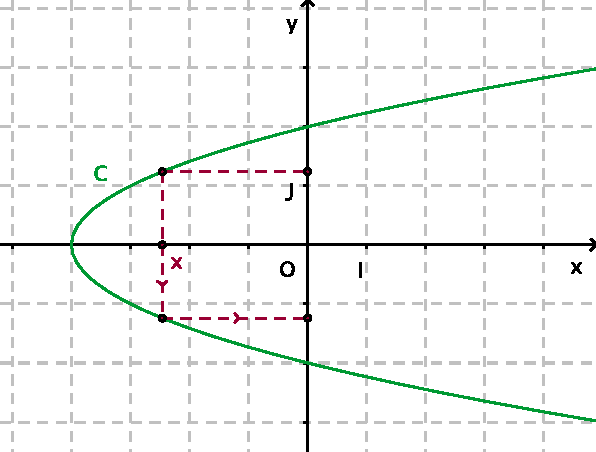
\includegraphics[width=5cm]{F_NonFct.pdf}

\begin{multicols}{2}
    Cette courbe ne représente pas une fonction, car à partir de \( x=-4\), les nombres ont deux images. Les courbes données par des fonctions sont des courbes acceptant une seule ordonnée pour chaque abscisse.

\columnbreak

%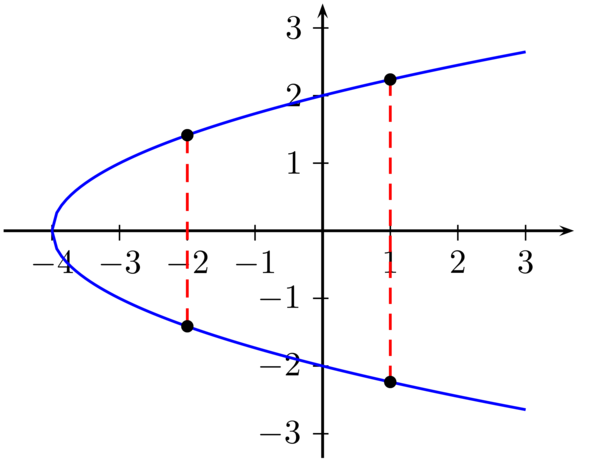
\includegraphics{Picture_FIGLabelFigPasFonctionYoQfSuPICTPasFonctionYoQfSu-for_eps.pdf}

\input{Fig_PasFonctionYoQfSu.pstricks}

\end{multicols}


Pour tracer le graphe d'une fonction affine.
\begin{itemize}
    \item
        Vu que le graphe est une droite, il suffit de deux points.
    \item
        Les fonction linéaires passent par l'origine \( (0;0)\).
    \item 
        Pour un tracé à la règle, il est plus précis de prendre deux points relativement éloignés.
    \item
        La droite \( f(x)=mx+p\) monte si \( m>0\) et descend si \( m<0\). La pente est d'autant plus raide que \( m\) est grand.
\end{itemize}

Quelque exemples à la figure \ref{LabelFigGrapheAffinHqXJGx}.
\newcommand{\CaptionFigGrapheAffinHqXJGx}{Des graphes de fonctions linéaires et affines.}
\input{Fig_GrapheAffinHqXJGx.pstricks}


\chapter{Rappels de géométrie}
% This is part of Un soupçon de mathématique sans être agressif pour autant
% Copyright (c) 2012
%   Laurent Claessens
% See the file fdl-1.3.txt for copying conditions.

%---------------------------------------------------------------------------------------------------------------------------
\subsection{Médianes, hauteurs, médiatrices}
%---------------------------------------------------------------------------------------------------------------------------

Soit un triangle \( ABC\).

%///////////////////////////////////////////////////////////////////////////////////////////////////////////////////////////
\subsubsection{Médianes}
%///////////////////////////////////////////////////////////////////////////////////////////////////////////////////////////

\begin{multicols}{2}
    Une médiane est une droite passant par le centre d'un des côtés et par le sommet opposé. Les trois médianes se coupent en un point nommé \defe{centre}{centre!d'un triangle}. Il est parfois aussi nommé \emph{centre de masse}. De plus le centre de masse du triangle est situé aux deux tiers de la hauteur ne partant du sommet :
    \begin{equation}
        \vect{ AG }=\frac{ 2 }{ 3 }\vect{ AI }.
    \end{equation}

    \columnbreak


%The result is on figure \ref{LabelFigfigureNPQwFTp}. % From file figureNPQwFTp
%\newcommand{\CaptionFigfigureNPQwFTp}{<+Type your caption here+>}
    \begin{center}
\input{Fig_figureNPQwFTp.pstricks}
    \end{center}

\end{multicols}

%///////////////////////////////////////////////////////////////////////////////////////////////////////////////////////////
\subsubsection{Hauteurs}
%///////////////////////////////////////////////////////////////////////////////////////////////////////////////////////////

\begin{multicols}{2}
    Une hauteur est une droite passant par un sommet et coupant perpendiculairement le côté opposé. Les trois hauteurs se coupent en un point appelé l'\defe{orthocentre}{orthocentre} du triangle, nomme \( H\).

    \columnbreak


%The result is on figure \ref{LabelFigfigureITVTofz}. % From file figureITVTofz
%\newcommand{\CaptionFigfigureITVTofz}{<+Type your caption here+>}
\input{Fig_figureITVTofz.pstricks}

\end{multicols}


%///////////////////////////////////////////////////////////////////////////////////////////////////////////////////////////
\subsubsection{Médiatrices}
%///////////////////////////////////////////////////////////////////////////////////////////////////////////////////////////

\begin{multicols}{2}
    Une médiatrice est une droite coupant une côté perpendiculairement à son milieu.

    \columnbreak

%The result is on figure \ref{LabelFigfigureNAKnjxQ}. % From file figureNAKnjxQ
%\newcommand{\CaptionFigfigureNAKnjxQ}{<+Type your caption here+>}
\input{Fig_figureNAKnjxQ.pstricks}

\end{multicols}

%///////////////////////////////////////////////////////////////////////////////////////////////////////////////////////////
\subsubsection{Droite d'Euler}
%///////////////////////////////////////////////////////////////////////////////////////////////////////////////////////////

<++>


%+++++++++++++++++++++++++++++++++++++++++++++++++++++++++++++++++++++++++++++++++++++++++++++++++++++++++++++++++++++++++++
\section{Triangles isométriques}
%+++++++++++++++++++++++++++++++++++++++++++++++++++++++++++++++++++++++++++++++++++++++++++++++++++++++++++++++++++++++++++

Voir \cite{TqcjwY}.

\begin{propriete}       \label{PropRtqqxJ}
    Soient les triangles \( ABC\) et \( MNP\). Si
    \begin{enumerate}
        \item
            \( \hat A=\hat M\)
        \item
            \( AB=MN\)
        \item
            \( AC=MP\)
    \end{enumerate}
    alors les triangles sont isométriques.

    Si
    \begin{enumerate}
        \item
            \( AB=MN\)
        \item
            \( \hat A=\hat M\)
        \item
            \( \hat B=\hat N\)
    \end{enumerate}
    alors les triangles sont isométriques.
\end{propriete}

%+++++++++++++++++++++++++++++++++++++++++++++++++++++++++++++++++++++++++++++++++++++++++++++++++++++++++++++++++++++++++++ 
\section{Exercices}
%+++++++++++++++++++++++++++++++++++++++++++++++++++++++++++++++++++++++++++++++++++++++++++++++++++++++++++++++++++++++++++


\Exo{Seconde-0045}
\Exo{smath-0010}


\chapter{Probabilités}
% This is part of Un soupçon de mathématique sans être agressif pour autant
% Copyright (c) 2013
%   Laurent Claessens
% See the file fdl-1.3.txt for copying conditions.

%+++++++++++++++++++++++++++++++++++++++++++++++++++++++++++++++++++++++++++++++++++++++++++++++++++++++++++++++++++++++++++ 
\section{Univers}
%+++++++++++++++++++++++++++++++++++++++++++++++++++++++++++++++++++++++++++++++++++++++++++++++++++++++++++++++++++++++++++

Nous allons fonder notre étude sur l'étude des trois expériences aléatoires.
\begin{enumerate}
    \item
        Lancer un dé à \( 6\) faces.
    \item
        Tirer une carte d'un jeu de \( 52\) cartes.
    \item
        Tirer une boule d'une urne contenant \( 16\) boules dont trois vertes, cinq jaunes, deux bleues et six rouges.
\end{enumerate}

\begin{definition}
    Une \defe{expérience aléatoire}{expérience aléatoire} est une expérience qui a plusieurs issues possibles, et pour laquelle on ne peut ni prévoir ni calculer laquelle des issues sera réalisée.
\end{definition}

\begin{definition}
    L'ensemble des issues possibles d'une expérience aléatoire est l'\defe{univers}{univers} de l'expérience. Il sera noté \( E\).
\end{definition}

\begin{enumerate}
    \item
        Lancer un dé à \( 6\) faces. L'univers est \( \{ 1,2,3,4,5,6 \}\).
    \item
        Tirer une carte d'un jeu de \( 52\) cartes. L'univers est \( \{ \text{as de pique},\text{cinq de carreau},\text{valet de trèfle}, \ldots \}\).
    \item
        Tirer une boule d'une urne qui contient par exemple trois boules vertes, cinq jaunes, deux bleues et six rouges. L'univers est \( \{ V,J,B,R \}\).
\end{enumerate}

%+++++++++++++++++++++++++++++++++++++++++++++++++++++++++++++++++++++++++++++++++++++++++++++++++++++++++++++++++++++++++++ 
\section{Événement}
%+++++++++++++++++++++++++++++++++++++++++++++++++++++++++++++++++++++++++++++++++++++++++++++++++++++++++++++++++++++++++++

\begin{definition}
    Un \defe{événement}{événement} d'une expérience aléatoire est une partie de l'univers : un sous-ensemble de l'ensemble des issues possibles. Un événement est \defe{élémentaire}{événement=élémentaire} si il n'est réalisé que par une seule issue de l'expérience.
\end{definition}

\begin{example}
    \begin{description}
        \item[Pour le dé]
            \begin{itemize}
                \item Obtenir le six (événement élémentaire).
                \item
                    Obtenir un nombre pair.
                \item
                    Obtenir \( 2\) ou \( 5\).
            \end{itemize}
        \item[Pour le jeu de cartes]
    \begin{itemize}
        \item
            Tirer le six de cœur (événement élémentaire).
        \item Tirer une carte noire.
        \item
            Tirer une dame.
    \end{itemize}
\item[Pour l'urne]
    \begin{itemize}
        \item Tirer une boule rouge (événement élémentaire).
        \item
            Tirer une boule rouge ou verte.
        \item
            Tirer une boule d'une couleur autre que verte.
    \end{itemize}
    \end{description}
\end{example}

%+++++++++++++++++++++++++++++++++++++++++++++++++++++++++++++++++++++++++++++++++++++++++++++++++++++++++++++++++++++++++++ 
\section{Probabilité}
%+++++++++++++++++++++++++++++++++++++++++++++++++++++++++++++++++++++++++++++++++++++++++++++++++++++++++++++++++++++++++++

Si nous recommençons plusieurs fois une même expérience aléatoire, nous pouvons parler de \defe{fréquence}{fréquence} d'apparition de l'événement \( A\).

\begin{definition}
    Lorsqu'on effectue un grand nombre de fois une expérience aléatoire, la fréquence d'apparition d'un événement \( A\) tend à se stabiliser autour d'une «fréquence théorique» appelée la \defe{probabilité}{probabilité} de \( A\) et notée \( p(A)\).
\end{definition}

\begin{example}
    Si \( A\) désigne l'événement «obtenir la face \( 4\) » lors du lancé du dé à \( 6\) faces, la probabilité est \( p(A)=\frac{1}{ 6 }\) parce que nous nous attendons à obtenir le \( 4\) une fois sur six.

    Si \( B\) désigne l'événement «obtenir un nombre pair», alors la probabilité est \( p(A)=\frac{ 1 }{2}\) parce qu'un lancer sur deux doit en moyenne tomber sur un nombre pair.
\end{example}

\begin{example}
    Si l'événement \( A\) désigne «obtenir l'as de $\spadesuit$», alors la probabilité est de \( 1/52\).
    
    Si \( B\) désigne l'événement «obtenir une dame», alors la probabilité est de \( 4/52=1/13\).
\end{example}

\begin{example}
    L'urne contient en tout \( 16\) boules. Nous avons
    \begin{itemize}
        \item \( p(V)=\frac{ 3 }{ 16 }\);
        \item
            \( p(R)=\frac{ 6 }{ 16 }=\frac{ 3 }{ 8 }\);
        \item
            \( p(B)=\frac{ 2 }{ 16 }=\frac{1}{ 8 }\).
    \end{itemize}
    
\end{example}


\begin{propriete}
    \begin{enumerate}
        \item
            Une probabilité est un nombre compris entre \( 0\) et \( 1\) : \( 0\leq p(A)\leq 1\).
        \item
            Un événement impossible a une probabilité \( 0\) : \( p(\emptyset)=0\).
        \item
            Un événement dont la probabilité est \( 1\) est appelé \defe{événement certain}{événement!certain}.
        \item
            La somme des probabilités de tous les événements élémentaires vaut toujours \( 1\).
    \end{enumerate}
\end{propriete}

\begin{definition}
    Lorsque tous les événements élémentaires ont la même probabilité, nous disons que nous sommes dans une situation d'\defe{équiprobabilité}{équiprobabilité}.
\end{definition}

\begin{propriete}
    Si une expérience possède \( n\) issues équiprobables, alors :
    \begin{enumerate}
        \item
            La probabilité de chaque événement primaire est \( \frac{1}{ n }\).
        \item
            La probabilité d'un événement \( A\) est donnée par
            \begin{equation}
                p(A)=\frac{ \Card(A) }{ n }
            \end{equation}
            où \( \Card(A)\) est le \defe{cardinal}{cardinal} de \( A\), c'est à dire le nombre d'éléments dans \( A\).
    \end{enumerate}
\end{propriete}

\begin{example}
    \begin{description}
        \item[Le dé à 6 faces]
            La probabilité d'un événement élémentaire est \( \frac{1}{ 6 }\).

            Si \( A\) est l'événement «obtenir un nombre pair», alors \( p(A)=\frac{ 3 }{ 6 }=\frac{ 1 }{2}\) parce qu'il y a trois nombres pairs : \( 2\), \( 4\) et \( 6\). Il y a donc trois issues possibles qui réalisent l'événement \( A\).
        \item[Le jeu de carte]
            Les événements élémentaires sont chacune des cartes et leurs probabilités sont \( \frac{1}{ 52 }\). 
            
            
            Si \( A\) est l'événement «Tirer une carte de \( \heartsuit\)», alors \( p(A)=\frac{ 13 }{ 52 }=\frac{1}{ 4 }\) parce qu'il y a \( 13\) cartes de \( \heartsuit\) sur \( 52\) cartes en tout.

        \item[L'urne] Les événements élémentaires (tirer une boule verte, jaune, bleue ou rouge) ne sont pas équiprobables. Par exemple la probabilité d'avoir une rouge est \( p(R)=\frac{ 6 }{ 16 }=\frac{ 3 }{ 8 }\).

            Si \( A\) est l'événement «tirer une boule jaune ou verte», alors nous avons \( p(A)=\frac{ 5+3 }{ 16 }=\frac{ 1 }{ 2 }\).
    \end{description}
\end{example}

\begin{definition}
    Si \( A\) est un événement, l'\defe{événement contraire}{événement!contraire}, noté \( \bar A\), est l'événement constitué de l'ensemble des événement élémentaires n'appartenant pas à \( A\). On a l'égalité
    \begin{equation}
        p(\bar A)=1-p(A).
    \end{equation}
\end{definition}

\begin{example}
    \begin{description}
        \item[Le dé à six face] Si \( A\) est l'événement «obtenir \( 3\) ou \( 4\)», alors \( \bar A\) est l'événement «ne pas obtenir \( 3\) ou \( 4\)», c'est à dire «obtenir \( 1\), \( 2\), \( 5\) ou \( 6\)».
        \item[Le jeu de cartes] Si \( A\) est l'événement «tirer un \( \spadesuit\)», alors l'événement contraire \( \bar A\) est l'événement «Tirer un \( \heartsuit\), \( \diamondsuit\) ou \( \clubsuit\)».
        \item[L'urne] Si \( A\) est l'événement «Tirer une boule verte ou jaune», alors le complémentaire est \( \bar A\) «Tirer une boule bleue ou rouge».
    \end{description}
\end{example}

%+++++++++++++++++++++++++++++++++++++++++++++++++++++++++++++++++++++++++++++++++++++++++++++++++++++++++++++++++++++++++++ 
\section{Réunion et intersection}
%+++++++++++++++++++++++++++++++++++++++++++++++++++++++++++++++++++++++++++++++++++++++++++++++++++++++++++++++++++++++++++

%TODO : des dessins pour expliquer la réunion et l'intersection.

Si \( A\) et \( B\) sont des événements, 
\begin{enumerate}
    \item
nous notons \( A\cup B\) l'événement qui est réalisé lorsque \( A\) \emph{ou} \( B\) se réalise;
\item
nous notons \( A\cap B\) l'événement qui est réalisé lorsque \( A\) \emph{et} \( B\) se réalisent.
\end{enumerate}

\begin{Aretenir}
    Si \( A\) et \( B\) sont deux événements d'une expérience aléatoire, alors
    \begin{equation}
        p(A\cup B)=p(A)+p(B)-p(A\cap B).
    \end{equation}
\end{Aretenir}

\begin{example}
    Soient \( A\) l'événement «obtenir un roi» et \( B\) l'événement «obtenir un \( \heartsuit\)». Pour calculer \( p(A\cup B)\), on suit le raisonnement suivant.
    \begin{enumerate}
        \item
            La probabilité de \( A\) est \( p(A)=\frac{ 4 }{ 52 }=\frac{1}{ 13 }\). 
        \item
            La probabilité de \( B\) est \( p(B)=\frac{ 13 }{ 52 }=\frac{1}{ 4 }\).
        \item
            L'événement \( A\cup B\) est l'événement «avoir un roi ou un cœur». Les cartes qui réalisent cet événement sont toutes les \( 13\) cartes de cœur plus les quatre rois (dont un est de cœur!!). 
        \item
            L'événement \( A\cap B\) est réalisé par les cartes qui sont à la fois cœur et roi, c'est à dire uniquement par la carte roi de \( \heartsuit\). Nous avons donc \( p(A\cap B)=\frac{1}{ 52 }\).
        \item
            Pour savoir la probabilité \( p(A\cup B)\), on utilise la formule
            \begin{equation}
                p(A\cup B)=p(A)+p(B)-p(A\cap B)=\frac{1}{ 13 }+\frac{1}{ 4 }-\frac{1}{ 52 }=\frac{ 4 }{ 13 }.
            \end{equation}
    \end{enumerate}
    Notons que ce résultat peut aussi être obtenu en réfléchissant. L'événement \( A\cup B\) est constitué de toutes les cartes \( \heartsuit\) et de tous les rois, c'est à dire les treize cartes \( \heartsuit\) plus les rois de \( \clubsuit\), \( \spadesuit\) et \( \diamondsuit\), soient \( 13+3=16\) cartes en tout. Donc
    \begin{equation}
        p(A\cup B)=\frac{ 16 }{ 52 }=\frac{ 4 }{ 13 }.
    \end{equation}
\end{example}

%+++++++++++++++++++++++++++++++++++++++++++++++++++++++++++++++++++++++++++++++++++++++++++++++++++++++++++++++++++++++++++ 
\section{Exercices}
%+++++++++++++++++++++++++++++++++++++++++++++++++++++++++++++++++++++++++++++++++++++++++++++++++++++++++++++++++++++++++++

\Exo{smath-0191}

%--------------------------------------------------------------------------------------------------------------------------- 
\subsection{Univers}
%---------------------------------------------------------------------------------------------------------------------------

\Exo{smath-0197}

%--------------------------------------------------------------------------------------------------------------------------- 
\subsection{Probabilités}
%---------------------------------------------------------------------------------------------------------------------------

\Exo{smath-0187}
\Exo{smath-0189}
\Exo{smath-0190}

%--------------------------------------------------------------------------------------------------------------------------- 
\subsection{Réunion, intersection}
%---------------------------------------------------------------------------------------------------------------------------

\Exo{smath-0215}
\Exo{smath-0214}
\Exo{smath-0280}
\Exo{smath-0287}
\Exo{smath-0347}

%--------------------------------------------------------------------------------------------------------------------------- 
\subsection{Modèles}
%---------------------------------------------------------------------------------------------------------------------------

\Exo{smath-0194}
\Exo{smath-0195}

%--------------------------------------------------------------------------------------------------------------------------- 
\subsection{Problèmes}
%---------------------------------------------------------------------------------------------------------------------------

\Exo{smath-0192}
\Exo{smath-0198}
\Exo{smath-0188}
\Exo{smath-0279}
\Exo{smath-0281}
\Exo{smath-0282}

%--------------------------------------------------------------------------------------------------------------------------- 
\subsection{Questions de cours}
%---------------------------------------------------------------------------------------------------------------------------

\Exo{smath-0184}



\chapter{La fonction inverse}
% This is part of Un soupçon de mathématique sans être agressif pour autant
% Copyright (c) 2013
%   Laurent Claessens
% See the file fdl-1.3.txt for copying conditions.

%+++++++++++++++++++++++++++++++++++++++++++++++++++++++++++++++++++++++++++++++++++++++++++++++++++++++++++++++++++++++++++ 
\section{Graphe et tableau de variation}
%+++++++++++++++++++++++++++++++++++++++++++++++++++++++++++++++++++++++++++++++++++++++++++++++++++++++++++++++++++++++++++

La fonction inverse est la fonction définie sur \( \eR\setminus\{ 0 \}\) qui à \( x\) fait correspondre \( \frac{1}{ x }\).

Son graphe et son tableau de variation les suivants : 
\begin{multicols}{2}

\begin{equation*}
    \begin{array}[]{ccccccc}
        -\infty&&&0&&&+\infty\\
        \hline
        0&&&|&+\infty&&\\
        &\searrow&&|&&\searrow&\\
        &&-\infty&|&&&0\\
    \end{array}
\end{equation*}

\columnbreak

%The result is on figure \ref{LabelFigfigureMIdFCNN}. % From file figureMIdFCNN
%\newcommand{\CaptionFigfigureMIdFCNN}{<+Type your caption here+>}
\begin{center}
\input{Fig_figureMIdFCNN.pstricks}
\end{center}
\end{multicols}

L'ensemble de définition de la fonction \( x\mapsto \frac{1}{ x }\) est l'ensemble de tous les réels sauf \( x=0\).

\begin{definition}
    La courbe représentative de la fonction inverse est nommée \defe{hyperbole}{hyperbole}.
\end{definition}

%+++++++++++++++++++++++++++++++++++++++++++++++++++++++++++++++++++++++++++++++++++++++++++++++++++++++++++++++++++++++++++ 
\section{Exercices}
%+++++++++++++++++++++++++++++++++++++++++++++++++++++++++++++++++++++++++++++++++++++++++++++++++++++++++++++++++++++++++++

% Il faut un peu reclasser ces exercices.

\Exo{smath-0256}
\Exo{smath-0262}
\Exo{smath-0257}
\Exo{smath-0258}

\Exo{smath-0369}
\Exo{smath-0350}
\Exo{smath-0260}
\Exo{smath-0259}
\Exo{smath-0261}
\Exo{smath-0265}
\Exo{smath-0268}
\Exo{smath-0272}
\Exo{smath-0273}
\Exo{smath-0274} 
\Exo{smath-0275}
\Exo{smath-0276}
\Exo{smath-0277}
\Exo{smath-0278}
\Exo{smath-0292}
\Exo{smath-0294}
\Exo{smath-0346}
\Exo{smath-0364}



\chapter{Configurations du plan}
% This is part of Un soupçon de mathématique sans être agressif pour autant
% Copyright (c) 2013
%   Laurent Claessens
% See the file fdl-1.3.txt for copying conditions.




\chapter{Fonctions homographiques}
%This is part of Un soupçon de mathématique sans être agressif pour autant
% Copyright (c) 2013
%   Laurent Claessens
% See the file fdl-1.3.txt for copying conditions.

%+++++++++++++++++++++++++++++++++++++++++++++++++++++++++++++++++++++++++++++++++++++++++++++++++++++++++++++++++++++++++++ 
\section{Définitions}
%+++++++++++++++++++++++++++++++++++++++++++++++++++++++++++++++++++++++++++++++++++++++++++++++++++++++++++++++++++++++++++

\begin{definition}
    Une \defe{fonction homographique}{homographique} est une fonction de la forme
    \begin{equation}
        f(x)=\frac{ ax+b }{ cx+d }.
    \end{equation}
Son domaine de définition est l'ensemble des \( x\in \eR\) tels que \( cx+d\neq 0\).
\end{definition}

%+++++++++++++++++++++++++++++++++++++++++++++++++++++++++++++++++++++++++++++++++++++++++++++++++++++++++++++++++++++++++++ 
\section{Exercices}
%+++++++++++++++++++++++++++++++++++++++++++++++++++++++++++++++++++++++++++++++++++++++++++++++++++++++++++++++++++++++++++

%AFAIRE : est-ce que ce newpage est encore utile ? et l'autre, en-dessous.
\newpage
\Exo{smath-0334}

\clearpage
\Exo{smath-0379}
\Exo{smath-0368}
\Exo{smath-0137}
\Exo{smath-0144}
\Exo{smath-0316}
\Exo{smath-0335}
\Exo{smath-0336}
\Exo{smath-0377}


\chapter{Trigonométrie}
% This is part of Un soupçon de mathématique sans être agressif pour autant
% Copyright (c) 2013
%   Laurent Claessens
% See the file fdl-1.3.txt for copying conditions.

%+++++++++++++++++++++++++++++++++++++++++++++++++++++++++++++++++++++++++++++++++++++++++++++++++++++++++++++++++++++++++++ 
\section{Enroulement de la droite numérique sur le cercle}
%+++++++++++++++++++++++++++++++++++++++++++++++++++++++++++++++++++++++++++++++++++++++++++++++++++++++++++++++++++++++++++

\begin{definition}
    Le \defe{cercle trigonométrique}{cercle!trigonométrique} est le cercle de centre \( (0;0)\) et de rayon \( 1\) muni de l'orientation dans le sens direct (le sens inverse des aiguilles d'une montre).
\end{definition}

Nous enroulons la droite réelle sur le cercle, voir la figure \ref{LabelFigYORfWSM}. % From file YORfWSM
\newcommand{\CaptionFigYORfWSM}{Un cercle trigonométrique avec enroulement de la droite rélle.}
\input{Fig_YORfWSM.pstricks}

Étant donné que la circonférence du cercle est \( 2\pi\), le nombre \( 2\pi\) de la droite réelle vient au même endroit que le nombre zéro. Le nombre \( 2\pi+x\) vient alors au même endroit que \( x\) pour tout \( x\).

%+++++++++++++++++++++++++++++++++++++++++++++++++++++++++++++++++++++++++++++++++++++++++++++++++++++++++++++++++++++++++++ 
\section{Cosinus et sinus}
%+++++++++++++++++++++++++++++++++++++++++++++++++++++++++++++++++++++++++++++++++++++++++++++++++++++++++++++++++++++++++++

\begin{minipage}{0.485\textwidth}
\begin{definition}
    Soit le réel \( x\) et le point image \( M\) sur le cercle trigonométrique. Le \defe{cosinus}{cosinus} de \( x\) est l'abscisse du point \( M\) et le \defe{sinus}{sinus} de \(x\) est l'ordonnée du point \( M\).
\end{definition}
\end{minipage}
\hspace{1mm}
\begin{minipage}{6cm}
    \begin{center}
   \input{Fig_LOBVHYF.pstricks}
    \end{center}
\end{minipage}

\begin{propriete}
    Vu que \( \big( \cos(x),\sin(x) \big)\) sont le coordonnées de points sur le cercle trigonométrique, nous avons
    \begin{enumerate}
        \item
            \( -1\leq \cos(x)\leq 1\)
        \item
            \( -1\leq \sin(x)\leq 1\)
        \item
            \( \cos^2(x)+\sin^2(x)=1\).
    \end{enumerate}
\end{propriete}

\begin{propriete}
    Pour tout réel \( x\), nous avons
    \begin{enumerate}
        \item
            \( \cos(-x)=\cos(x)\)
        \item
        \( \sin(-x)=-\sin(x)\)
    \end{enumerate}
\end{propriete}
Cette propriété est due au fait que les points \( x\) et \( -x\) de l'axe réel viennent se placer sur le cercle trigonométrique sur des points symétriques par rapport à l'axe horizontal.

%+++++++++++++++++++++++++++++++++++++++++++++++++++++++++++++++++++++++++++++++++++++++++++++++++++++++++++++++++++++++++++ 
\section{Exercices}
%+++++++++++++++++++++++++++++++++++++++++++++++++++++++++++++++++++++++++++++++++++++++++++++++++++++++++++++++++++++++++++

\Exo{smath-0360}
\Exo{smath-0361}
\Exo{smath-0362}
\Exo{smath-0363}
\Exo{smath-0366}
\Exo{smath-0367}
\Exo{smath-0373}


\chapter{Algorithmique}
% This is part of Un soupçon de mathématique sans être agressif pour autant
% Copyright (c) 2012
%   Laurent Claessens
% See the file fdl-1.3.txt for copying conditions.

Pour ce chapitre, nous suivons entre autres \cite{oklaEg}.

Ce chapitre ne contient pas de théorie particulière. Seulement de la pratique. Le exemples seront écrits en python; en dehors des séances effectuées sur ordinateur, les élèves ne sont pas obligés de maîtriser la syntaxe exacte.


%--------------------------------------------------------------------------------------------------------------------------- 
\subsection{Choses basiques}
%---------------------------------------------------------------------------------------------------------------------------

\Exo{smath-0118}
\Exo{Seconde-0018}
\Exo{smath-0037}

%--------------------------------------------------------------------------------------------------------------------------- 
\subsection{Instructions conditionnelles}
%---------------------------------------------------------------------------------------------------------------------------

\Exo{smath-0119}
\Exo{smath-0171}
\Exo{smath-0172}
\Exo{smath-0173}

%--------------------------------------------------------------------------------------------------------------------------- 
\subsection{Boucles}
%---------------------------------------------------------------------------------------------------------------------------


\Exo{smath-0181}
\Exo{smath-0182}
\Exo{smath-0183}
\Exo{smath-0202}


%--------------------------------------------------------------------------------------------------------------------------- 
\subsection{Autres}
%---------------------------------------------------------------------------------------------------------------------------

\Exo{smath-0002}
\Exo{smath-0003}
\Exo{Seconde-0086}
\Exo{smath-0007}
\Exo{smath-0008}



\chapter{Les épaves}
% This is part of Un soupçon de mathématique sans être agressif pour autant
% Copyright (c) 2012-2013
%   Laurent Claessens
% See the file fdl-1.3.txt for copying conditions.

Ce chapitre contient les choses tapées mais qui sont hors programmes.

%+++++++++++++++++++++++++++++++++++++++++++++++++++++++++++++++++++++++++++++++++++++++++++++++++++++++++++++++++++++++++++ 
\section{Statistique descriptive}
%+++++++++++++++++++++++++++++++++++++++++++++++++++++++++++++++++++++++++++++++++++++++++++++++++++++++++++++++++++++++++++

%--------------------------------------------------------------------------------------------------------------------------- 
\subsection{Activité : mois de naissance}
%---------------------------------------------------------------------------------------------------------------------------

Prendre les mois de naissance des élèves, en séparant les groupes.
\begin{enumerate}
    \item
        Quel groupe a la proportion de naissance en mars la plus grande ?
    \item
        En tout quelle est la proportion des naissances en avril ?
    \item 
        Est-ce qu'on peut voir l'effet comme quoi les mois de \( 31\) jours son plus longs ? 
        \begin{enumerate}
            \item
                Quelle est la proportion d'élèves nés dans un mois de \( 31\) jours ?
            \item
                Il y a \( 7\) mois de $31$ jours contre \( 5\) de moins. Donc le résultat est biaisé.
            \item
                Calculer la \emph{fréquence} des naissances en naissances par mois.
        \end{enumerate}
\end{enumerate}


\begin{example}
    Comment manipuler des chiffres et la perception des coefficients des épreuves du bac. en utilisant à tort et à travers la notion de moyenne ?\\
    \url{http://allken-bernard.org/pierre/weblog/?p=2386}
\end{example}



\begin{definition}
    Une \defe{population}{population} est un ensemble fini. Une \defe{série statistique}{série statistique} sur une population est une fonction qui à chaque élément (individu) de la population fait correspondre une valeur.

    L'\defe{effectif}{effectif} d'une valeur est le nombre d'individus correspondant à la valeur.

    La \defe{fréquence}{fréquence} d'une valeur est le rapport
    \begin{equation}
        f=\frac{ \text{effectif de la valeur} }{ \text{effectif total} }
    \end{equation}
    où par «effectif total» nous entendons la taille de la population totale.
\end{definition}

La \defe{moyenne}{moyenne} d'une suite de nombres \( x_1,\ldots, x_n\) est
\begin{equation}
    \bar x=\frac{1}{ n }\sum_{i=1}^nx_i=\frac{ \text{somme des \( x_i\)} }{\text{nombre de données}}.
\end{equation}

\begin{example}
    Soit la suite de nombres
    \begin{equation}
        1,7,0,3,9,0,1,3,1,0,2,5,6,9,1,1,3,2,4.
    \end{equation}
    Il y a \( 19\) nombres. La moyenne est donnée par la fraction
    \begin{equation}
        \bar x=\frac{ 1+7+0+3+9+\ldots+3+2+4 }{ 19 }=\frac{ 58 }{ 19 }.
    \end{equation}

Python permet d'obtenir assez facilement une approximation numérique :
    \begin{verbatim}
>>> import numpy
>>> nombres=[1,7,0,3,9,0,1,3,1,0,2,5,6,9,1,1,3,2,4]
>>> numpy.mean(nombres)          # 'mean' signifie 'moyenne' en anglais.
3.0526315789473686 
    \end{verbatim}
\end{example}


%+++++++++++++++++++++++++++++++++++++++++++++++++++++++++++++++++++++++++++++++++++++++++++++++++++++++++++++++++++++++++++
\section{Dessiner en vraie grandeur}
%+++++++++++++++++++++++++++++++++++++++++++++++++++++++++++++++++++++++++++++++++++++++++++++++++++++++++++++++++++++++++++

La perspective cavalière n'est pas parfaite; aucune perspective n'est parfaite. Étant donné que les surfaces sont déformées, nous voudrions être capables de dessiner certaines surfaces sans déformations. C'est ce que nous appelons \emph{dessiner en vraie grandeur}.

\begin{Aretenir}
    Lorsqu'on demande de dessiner une surface en vraie grandeur, voici les mouvements «de base» que vous êtes autorisés à effectuer \emph{dans un plan}.
    \begin{enumerate}
        \item
            Tracer des segments de longueur \emph{entières} !
        \item
            Tracer des cercles dont le centre et un point sont donnés.
        \item
            Tracer les droites dont deux points sont donnés.
        \item
            Considérer les intersections des droites et cercles.
    \end{enumerate}
    À partir ce ces mouvements, il est possible de tracer de nombreuses choses, dont par exemple
    \begin{enumerate}
        \item
            Le milieu du segment \( [AB]\) lorsque les points \( A\) et \( B\) sont donnés.
        \item
            Si la droite \( d\) et le point \( I\) plan sont donnés, la perpendiculaire à \( d\) passant par \( I\).
        \item
            Si les points \( d\) du plan et le point \( I\) sont donnés, la parallèle à \( d\) passant par \( I\).
    \end{enumerate}
\end{Aretenir}

\begin{proof}
    Nous allons donner les constructions.
    \begin{enumerate}
        \item
            Soient \( A\) et \( B\) données. À construire : la médiatrice du segment \( [AB]\). Avec cela, nous connaîtrons le milieu. Le technique est simple : il suffit de tracer deux cercles de même rayons \( r\) centrés en \( A\) et en \( B\). Les points d'intersection \( I\) et \( J\) donnent la médiatrice. En effet, par construction \( I\) est équidistant de \( A\) et \( B\) parce que \( I\) est à la fois sur le cercle de rayon \( r\) autour de \( A\) et sur le cercle de rayon \( r\) autour de \( B\). Or nous savons que les points équidistants de \( A\) et \( B\) sont sur la médiatrice du segment \( [AB]\).

            Pour la même raison, le point \( J\) est également sur la médiatrice. Cela fait que \( (IJ)\) coupe \( [AB]\) en son milieu.

Cette construction est illustrée sur la figure \ref{LabelFigIsoceleVdviOE}. % From file IsoceleVdviOE
\newcommand{\CaptionFigIsoceleVdviOE}{Le triangle \( AJB\) est isocèle.}
\input{Fig_IsoceleVdviOE.pstricks}

        \item

            Soient donnés la droite \( d\) et le point \( I\). Nous construisons un cercle centré en \( I\) et nous nommons \( A\) et $B$ les points d'intersection entre ce cercle et la droite \( A\). Par construction le triangle \( AIB\) est isocèle. Donc \( I\) est sur la médiatrice du segment \( [AB]\). La construction précédente permet de construire cette médiatrice qui sera alors perpendiculaire à \( d\) passant par \( I\).

Un dessin de la situation est proposé à la figure \ref{LabelFigPerpSegqrbMBZ}. % From file PerpSegqrbMBZ
\newcommand{\CaptionFigPerpSegqrbMBZ}{Le triangle \( AIB\) est isocèle et la droite rouge est la médiatrice de \( [AB]\).}
\input{Fig_PerpSegqrbMBZ.pstricks}

    \item
        
        Si la droite \( d\) et le point \( I\) sont donnés, pour construire la parallèle à \( d\) passant par \( I\), il suffit de construire la perpendiculaire \( d'\) à \( d\) passant par \( I\) et ensuite la perpendiculaire à \( d'\) passant par \( I\).

    \end{enumerate}
\end{proof}


Quelque dessin qui ne sont plus utilisés :


Des exemples sont donnés à la figure \ref{LabelFigPositionsDroitesbnYIsH}. % From file PositionsDroitesbnYIsH
\newcommand{\CaptionFigPositionsDroitesbnYIsH}{Droites coplanaires ou non.}
\input{Fig_PositionsDroitesbnYIsH.pstricks}

%See also the subfigure \ref{LabelFigPositionsDroitesbnYIsHssLabelSubFigPositionsDroitesbnYIsH0}
%See also the subfigure \ref{LabelFigPositionsDroitesbnYIsHssLabelSubFigPositionsDroitesbnYIsH1}
%See also the subfigure \ref{LabelFigPositionsDroitesbnYIsHssLabelSubFigPositionsDroitesbnYIsH2}
Notez en particulier la figure \ref{LabelFigPositionsDroitesbnYIsHssLabelSubFigPositionsDroitesbnYIsH3} sur laquelle les droites \( (FH)\) et \( (AC)\) ne sont pas sécantes !


%+++++++++++++++++++++++++++++++++++++++++++++++++++++++++++++++++++++++++++++++++++++++++++++++++++++++++++++++++++++++++++ 
\section{Surfaces dans un cube}
%+++++++++++++++++++++++++++++++++++++++++++++++++++++++++++++++++++++++++++++++++++++++++++++++++++++++++++++++++++++++++++

La figure \ref{LabelFigDesSections} montre un cube. Êtes-vous capables de donner la nature des surfaces coloriées ?
\newcommand{\CaptionFigDesSections}{Exercice de vision dans l'espace.}
\input{Fig_DesSections.pstricks}
Le triangle vert est isocèle et rectangle parce que deux de ses côtés sont des arrêtes du cube. Le triangle rouge est plus troublant, mais il est équilatéral : ses trois côtés sont des diagonales des faces du cube. Notez que \emph{sur le dessin}, les trois côtés ont des longueur différentes.

%+++++++++++++++++++++++++++++++++++++++++++++++++++++++++++++++++++++++++++++++++++++++++++++++++++++++++++++++++++++++++++
\section{Les règles de la perspective cavalière}
%+++++++++++++++++++++++++++++++++++++++++++++++++++++++++++++++++++++++++++++++++++++++++++++++++++++++++++++++++++++++++++

Lorsque nous dessinons en trois dimension, nous prenons les conventions suivantes qui définissent la \defe{\wikipedia{fr}{Perspective_cavalière}{perspective cavalière}}{perspective!cavalière}.

\begin{Aretenir}
    D'abord nous choisissons
    \begin{enumerate}
        \item
            Nous choisissons un \defe{angle de fuite}{angle!de fuite} \( \alpha\) qui sera entre \unit{30}{\degree} et \( \unit{45}{\degree}\) avec l'horizontale\footnote{Sur une feuille à carreaux, le plus simple est de prendre \unit{45}{\degree}.}.
        \item
            Un \defe{coefficient de réduction}{coefficient de réduction} que nous noterons \( k\) et qui sera compris entre \( 0\) et \( 1\).
    \end{enumerate}

    Ensuite nous prenons les correspondances suivantes entre la réalité et le dessin :
    \begin{center}
        \begin{tabular}{|p{7.5cm}|p{7.5cm}|}
            \hline
            {\bf dans la réalité}&{\bf sur le dessin}\\
            \hline\hline
            Segment caché  & Segment pointillé\\
            \hline
            Segment parallèle à la feuille de dessin & Segment représenté en vraie grandeur\\
            \hline
            Segment perpendiculaire à la feuille de dessin & Segment faisant un angle \( \alpha\) avec l'horizontale.\\
            \hline
            Une arrête de longueur \( l\) perpendiculaire à la feuille de dessin & Une arrête de longueur \( k\times l\) faisant un angle \( \alpha\) avec l'horizontale.\\
            \hline
        \end{tabular}
    \end{center}
\end{Aretenir}

\begin{minipage}{0.485\textwidth}
    Un carré fait un demi-centimètre. 
    \begin{itemize}
        \item Quel est l'angle de fuite utilisé ?
        \item Quel est le coefficient de réduction utilisé ?
    \end{itemize}
\end{minipage}
\hspace{1mm}
\begin{minipage}{0.6\textwidth}
    \center
    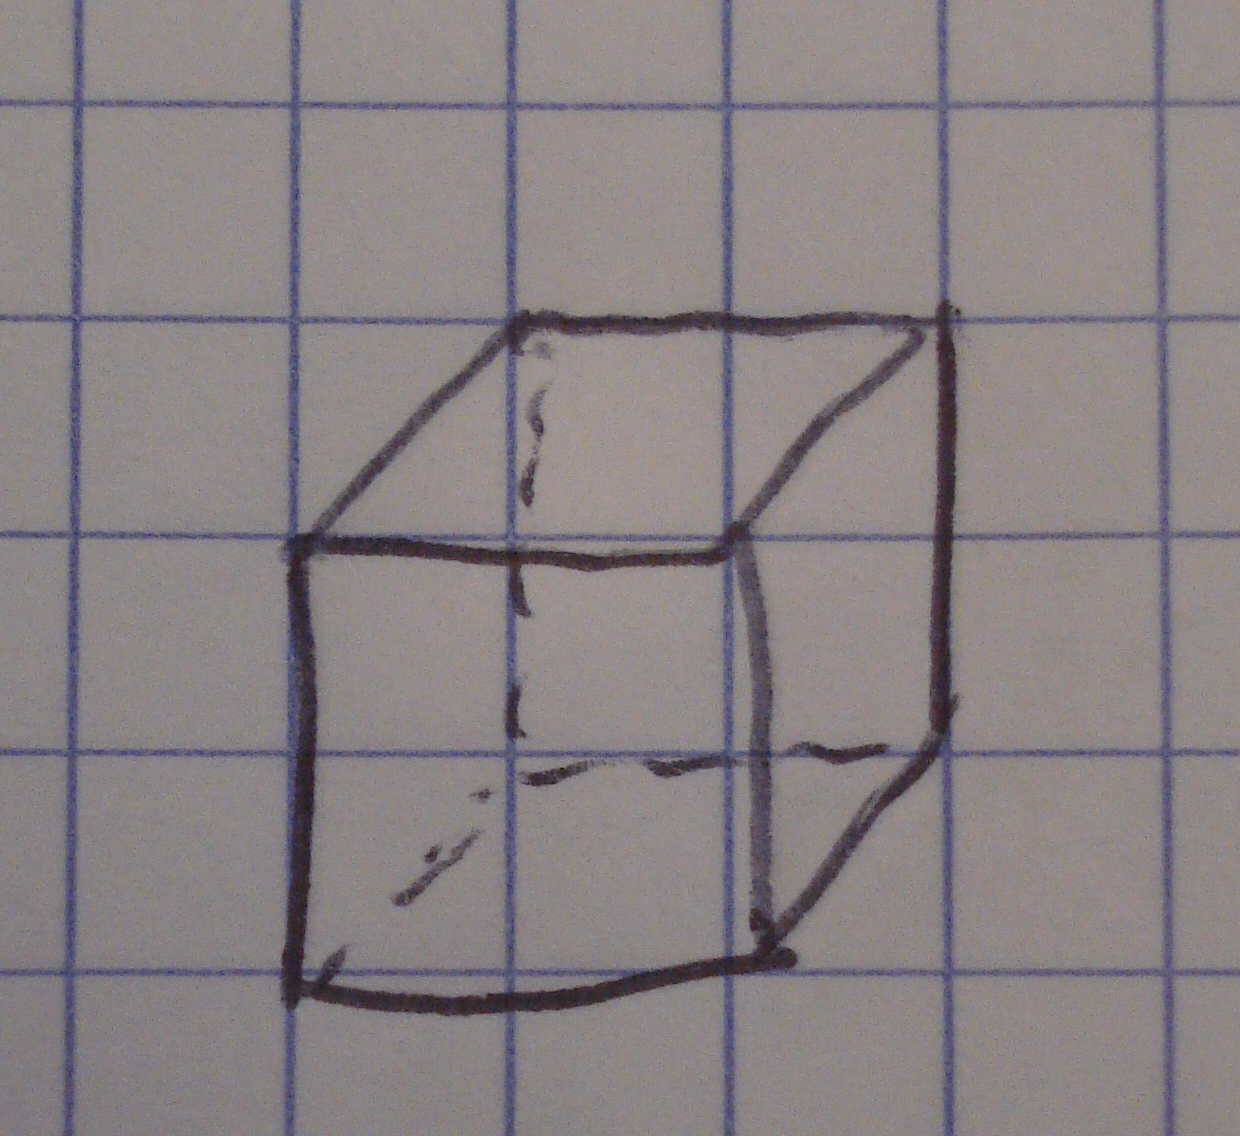
\includegraphics[width=0.6\textwidth]{cube_quadrill.png}
\end{minipage}

\begin{propriete}
    La perspective cavalière respecte les conditions suivantes.
    \begin{enumerate}
        \item
             Deux segments parallèles dans la réalité sont représentés par deux segments parallèles sur le dessin.
         \item
             Trois points alignés dans la réalité sont représentés par trois points alignés sur le dessin.
         \item
             Si \( M\) est le milieu du segment \( [AB]\) dans la réalité, alors \( M\) est le milieu du segment \( [AB]\) dans la réalité.
         \item
             La perspective cavalière respecte les proportions. C'est à dire que si le segment \( [AB]\) est \( p\) fois plus grand que le segment \( [CD]\) dans la réalité, alors il sera \( p\) fois plus grand sur le dessin.
    \end{enumerate}
\end{propriete}

Le cube de la figure \ref{LabelFigCubeLFZuiW} est dessiné avec \( \alpha=\unit{45}{\degree}\) et \( k=0.5\). Notez que les côtés parallèles restent parallèles.
\newcommand{\CaptionFigCubeLFZuiW}{Les segments perpendiculaires à la feuille sont de longueur moitié des autres.}
\input{Fig_CubeLFZuiW.pstricks}

La perspective cavalière n'est pas parfaite; il est aisé de créer des illusions d'optique comme celle de la figure \ref{LabelFigIllusionNHwEtp}. % From file IllusionNHwEtp
\newcommand{\CaptionFigIllusionNHwEtp}{Une petite illusion d'optique facile.}
\input{Fig_IllusionNHwEtp.pstricks}

%+++++++++++++++++++++++++++++++++++++++++++++++++++++++++++++++++++++++++++++++++++++++++++++++++++++++++++++++++++++++++++ 
\section{Exercices}
%+++++++++++++++++++++++++++++++++++++++++++++++++++++++++++++++++++++++++++++++++++++++++++++++++++++++++++++++++++++++++++

\Exo{Seconde-0096}
\Exo{Seconde-0097}

%+++++++++++++++++++++++++++++++++++++++++++++++++++++++++++++++++++++++++++++++++++++++++++++++++++++++++++++++++++++++++++ 
\section{AP sur les problèmes climatiques et de pétrole}
%+++++++++++++++++++++++++++++++++++++++++++++++++++++++++++++++++++++++++++++++++++++++++++++++++++++++++++++++++++++++++++

Je voudrais faire une AP basée sur la vidéo de Jean-Marc Jancovici à l'ENS :
\url{http://savoirsenmultimedia.ens.fr/expose.php?id=572}

Montrer ça à des élèves de seconde est le super-défi :)



%+++++++++++++++++++++++++++++++++++++++++++++++++++++++++++++++++++++++++++++++++++++++++++++++++++++++++++++++++++++++++++
\section{Regardons des graphiques}
%+++++++++++++++++++++++++++++++++++++++++++++++++++++++++++++++++++++++++++++++++++++++++++++++++++++++++++++++++++++++++++

Les graphiques sont souvent tirés de wikipédia. Si vous voulez plus d'informations, lisez \url{http://www.manicore.com/}, ou bien regardez le cours \href{http://www.mines-paristech.fr/ingenieurcivil/SitesIC/Balado/Climat_som.html}{en ligne}, en particulier la deuxième heure du troisième cours donne les facteurs d'émissions dans le monde et en France.

%---------------------------------------------------------------------------------------------------------------------------
\subsection{Émissions par secteurs}
%---------------------------------------------------------------------------------------------------------------------------

\EpsOrPdfincludegraphics[width=17cm]{Emission_de_GES}
Graphique en provenance de l'article \wikipedia{fr}{Gaz_à_effet_de_serre}{gaz à effet de serre} de wikipédia.

\begin{enumerate}
    \item
        Quel est le secteur qui émets le plus ?
    \item
        Est-ce que l'agriculture émet beaucoup de dioxyde de carbone ?
    \item
        À partir des deux graphiques du bas, est-ce que vous êtes capables de retrouver le \( 12.5\%\) de l'agriculture donnés dans le graphique du haut ?
\end{enumerate}

%---------------------------------------------------------------------------------------------------------------------------
\subsection{Découvertes de pétrole}
%---------------------------------------------------------------------------------------------------------------------------

Regardons un instant le graphique suivant, provenant de l'article \wikipedia{fr}{Pic_pétrolier}{Pic pétrolier} de wikipédia.

\EpsOrPdfincludegraphics[width=17cm]{Decouvertes-petrole}

\begin{enumerate}
    \item
        Quelle est l'année où on a découvert le plus de pétrole ?
    \item
        Quelle est l'année où on a consommé le plus de pétrole ?
    \item
        En quelles années on a consommé autant qu'on a découvert ?
    \item
        Que pensez-vous de l'affirmation «ce qui reste comme réserve est la surface jaune au-dessus de la ligne rouge» ?
\end{enumerate}
Pour aller plus loin, remarquer la cassure assez nette de la croissance de la production vers 1975. Juste par curiosité, faites quelque recherches sur l'histoire de la croissance économique, de la dette publique et le chômage en France (et en Europe). Est-ce que les années 1970 ont été spéciales de ce point de vue ?

%---------------------------------------------------------------------------------------------------------------------------
\subsection{Températures}
%---------------------------------------------------------------------------------------------------------------------------

\EpsOrPdfincludegraphics[width=17cm]{Instrumental_Temperature_Record_fr}
Graphique en provenance de l'article \wikipedia{fr}{Réchauffement_climatique}{réchauffement climatique} de wikipédia.

Le zéro de ce graphique est la moyenne 1961-1990.

\begin{enumerate}
    \item
        Quelle est la dernière année «normale» ?
    \item
        Quelle est l'année la plus chaude ?
    \item
        Quelle est l'année la plus froide ?
\end{enumerate}

%---------------------------------------------------------------------------------------------------------------------------
\subsection{Consommation de pétrole}
%---------------------------------------------------------------------------------------------------------------------------

Lire le tableau suivant :
\begin{center}
\begin{tabular}[h]{|c|c|c|c|c|c|c|c|c|}
année&
2001&
2002&
2003&
2004&
2005&
2006&
2007&
2008\\
consommation (Mb/j)&
76,8&
77,7&
79,1&
81,8&
83,1&
83,8&
84,9&
84,5
\end{tabular}
\end{center}

Calculer le pourcentage d'augmentation année par année. Que s'est-il passé en 2008 ?


%---------------------------------------------------------------------------------------------------------------------------
\subsection{Orthogonalité}
%---------------------------------------------------------------------------------------------------------------------------

% Note : l'orthogonalité n'a pas l'air d'être au programme de seconde.
\Exo{smath-0077}
\Exo{smath-0082}



%+++++++++++++++++++++++++++++++++++++++++++++++++++++++++++++++++++++++++++++++++++++++++++++++++++++++++++++++++++++++++++ 
\section{Intervalle de fluctuation}
%+++++++++++++++++++++++++++++++++++++++++++++++++++++++++++++++++++++++++++++++++++++++++++++++++++++++++++++++++++++++++++

Pour reprendre le cas de l'acné, nous considérons la population française totale (65 millions de personnes), et nous voulons savoir si les \emph{jelly bean} sont liés à l'acné.

Il n'est évidemment pas question de tester toute la France. L'étude est en plusieurs étapes.
\begin{enumerate}
    \item
        On va demander aux spécialistes quel est le pourcentage de français souffrant d'acné. Disons pour l'exemple que le résultat soit de \( 20\%\).
    \item
        On prend un échantillon de français (disons \( 1000\)) mangeant régulièrement des \emph{jelly beans}, et on compte combien ont de l'acné.
    \item
        Si plus de \( 20\%\) des personnes de l'échantillon présente de l'acné, alors on se pose des questions.
\end{enumerate}

Dans l'échantillon, nous nous attendons à avoir 
\begin{equation}
    \frac{ 20 }{ 100 }\times 1000=200
\end{equation}
personnes développant de l'acné si les \emph{jelly beans} ne sont pas liées à l'acné. 

Évidemment, si on en a \( 201\) ou \( 199\), ce n'est pas un problème. La question précise à laquelle nous devons répondre est :
\begin{quote}
    À partir de combien de personnes développant de l'acné, pouvons-nous dire que ça ne peut pas être le fruit du hasard ?
\end{quote}
Et c'est la réponse à cette questions que ne connaît manifestement pas le journaliste qui a écrit l'article en fin de blague.


Comment cela s'applique à notre étude de \emph{jelly bean} ? 
\begin{description}
    \item[Résumé des données]
        La proportion des français présentant de l'acné est dite de \( p=0.2\), et nous avons prélevé un échantillon de taille \( n=1000\). 
    \item[Intervalle de fluctuation] 
        Donc dans notre échantillon nous avons \( 95\%\) de chances que la fréquence soit dans l'intervalle
        \begin{equation}
            \mathopen[ 0.2-\frac{1}{ \sqrt{1000} } ; 0.2+\frac{1}{ \sqrt{1000} } \mathclose]\simeq\mathopen[ 0.168 ; 0.231 \mathclose]
        \end{equation}
        parce que \( \frac{1}{ \sqrt{1000} }\simeq 0.03162\).
    \item[Transformation en effectifs]

        Une fréquence de \( 0.168\) dans un échantillon de \( 1000\) individus revient à \( 168\) individus et une fréquence de \( 0.231\) revient à \( 231\) individus.

        Nous avons donc \( 95\%\) de chances que, en faisant l'étude sur \( 1000\) personnes, le nombre de personnes présentant de l'acné soit compris ente \( 168\) et \( 231\).
    \item[Décider si les \emph{jelly bean} provoquent l'acné]
        Si sur un échantillon de \( 1000\) personnes mangeant des \emph{jelly bean} nous en avons par exemple \( 260\) qui présentent de l'acné, alors nous pouvons dire que les \emph{jelly bean} sont liés à l'acné au sens où il y a moins de \( 5\%\) de chances que le résultats puisse s'expliquer par le hasard.

        Si sur cet échantillon de \( 1000\) personnes, nous en avons \( 180\), nous ne dirons rien. Avoir \( 180\) personnes avec de l'acné dans un échantillon de \( 1000\) personnes est «raisonnable» par rapport à la moyenne nationale.
\end{description}

\begin{remark}
    Dans le cas où le nombre de personnes présentant de l'acné dépasse les \( 231\), ça ne veut pas dire que les \emph{jelly bean} \emph{provoquent} l'acné. Cela veut juste dire qu'elles sont \emph{corrélées} à l'acné, et qu'il y a même \( 5\%\) de chances que ce soit un pur hasard.
\end{remark}


%+++++++++++++++++++++++++++++++++++++++++++++++++++++++++++++++++++++++++++++++++++++++++++++++++++++++++++++++++++++++++++ 
\section{Intervalle de confiance}
%+++++++++++++++++++++++++++++++++++++++++++++++++++++++++++++++++++++++++++++++++++++++++++++++++++++++++++++++++++++++++++

Nous avons vu l'intervalle de fluctuation. Il s'agit, lorsqu'on connaît la proportion \( p\) des individus présentant un certain caractère dans la population globale, de savoir si la fréquence $f$ observée dans un échantillon de taille \( n\) est crédible ou pas.

Ici nous allons poser la question inverse. Nous ne connaissons pas la proportion dans la population globale, mais seulement une fréquence dans un échantillon.

Soit donc une population dont une proportion inconnue \( p\) présente un caractère. Nous en tirons un échantillon de taille \( n\), et nous mesurons la fréquence \( f\) d'apparition du caractère dans cet échantillon.

Question : sachant \( f\), que peut-on dire de \( p\) ? 

Ce que nous savons, c'est qu'il y a \( 95\%\) de chances que 
\begin{equation}
    f\in\mathopen[ p-\frac{1}{ \sqrt{n}} , 1+\frac{1}{ \sqrt{n} } \mathclose].
\end{equation}
Cet intervalle peut être décortiqué de la façon suivante :
\begin{equation}
\xymatrix{%
    &   f\in\mathopen[ p-\frac{1}{ \sqrt{n}} , p+\frac{1}{ \sqrt{n} } \mathclose]\ar[rd]\ar[ld] &  \\
    f\geq p-\frac{1}{ \sqrt{n}}\ar[d]&&f\leq p+\frac{1}{ \sqrt{n}}  \ar[d]\\
    p\leq f+\frac{1}{ \sqrt{n}}\ar[rd] && f-\frac{1}{ \sqrt{n}}\leq p\ar[ld]\\
    & p\in\mathopen[ f-\frac{1}{ \sqrt{n} } , f+\frac{1}{ \sqrt{n}} \mathclose]  &
   }
\end{equation}

\begin{center}

           \ifpdf
            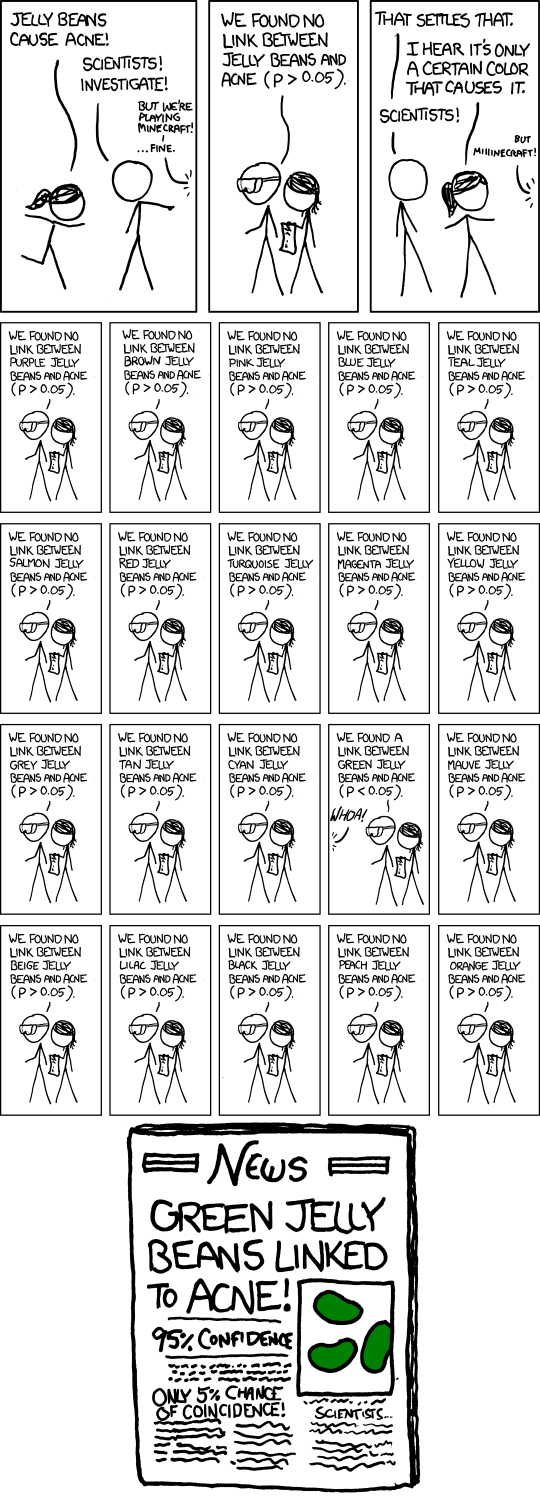
\includegraphics[width=8cm]{significant.png}
        \else
            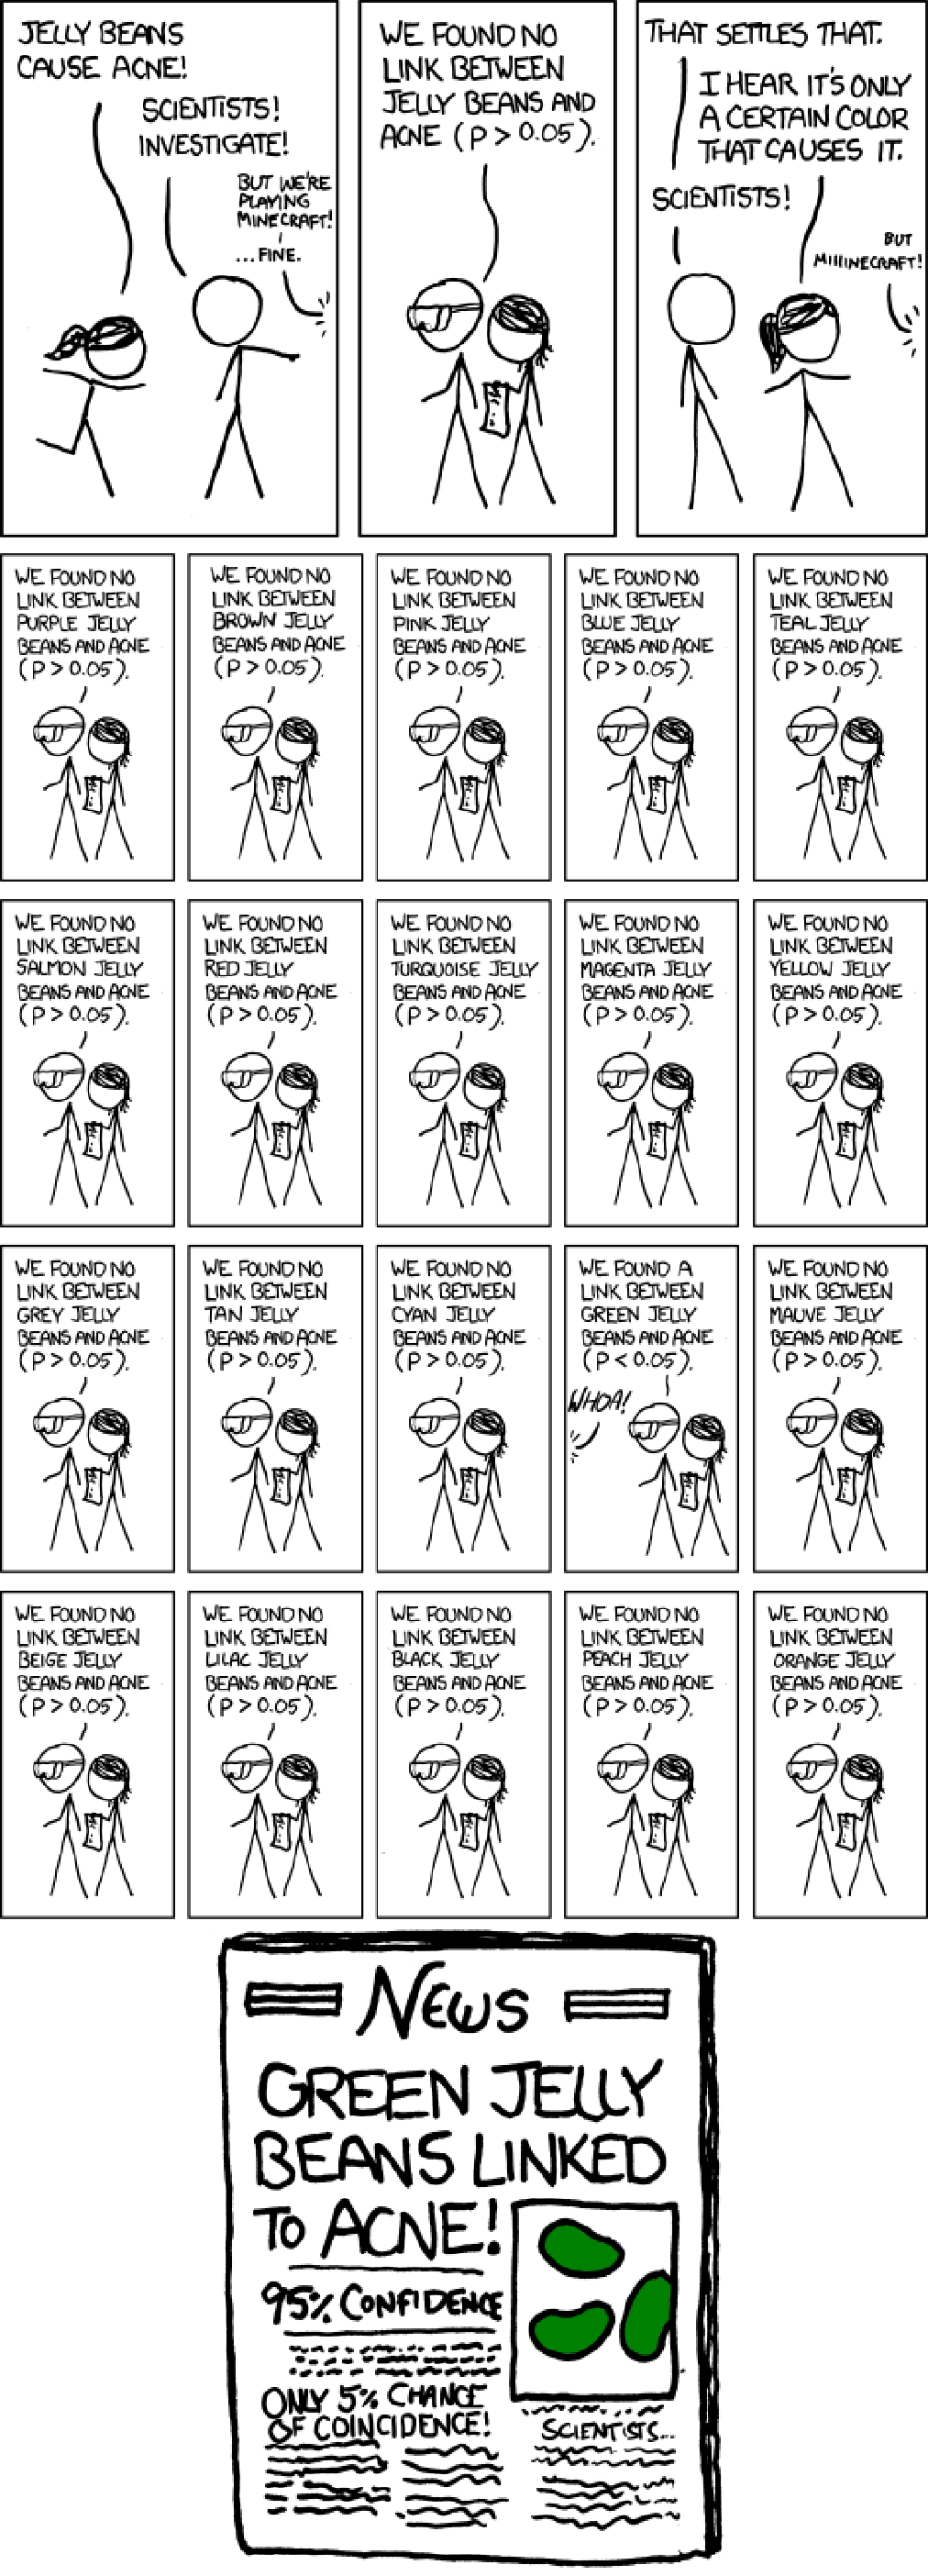
\includegraphics[width=8cm]{significant.eps}

            \fi

            \url{http://xkcd.com/882/}, image publiée sous licence \href{http://xkcd.com/license.html}{CreativeCommons}.

\end{center}

%+++++++++++++++++++++++++++++++++++++++++++++++++++++++++++++++++++++++++++++++++++++++++++++++++++++++++++++++++++++++++++ 
\section{Vecteurs}
%+++++++++++++++++++++++++++++++++++++++++++++++++++++++++++++++++++++++++++++++++++++++++++++++++++++++++++++++++++++++++++

\begin{propriete}
    Si \( \vect{ AB }=\vect{ CD }\) alors les translations \( t_{A,B}\) et \( t_{C,D}\) sont égales, c'est à dire que pour tout point \( K\) dans le plan, nous avons \( t_{A,B}(K)=t_{C,D}(K)\).
\end{propriete}

\begin{proof}
    L'égalité \( \vect{ AB }=\vect{ CD }\) nous dit immédiatement que \( ABDC\) est un parallélogramme. Soit \( K\) un point quelconque du plan et \( K'=t_{A,B}(K)\). Alors \( ABK'K\) est un parallélogramme. Nous devons prouver que \( CDK'K\) est également un parallélogramme. La situation est à la figure \ref{LabelFigVectoParallItzteT}. % From file VectoParallItzteT
\newcommand{\CaptionFigVectoParallItzteT}{Nous savons que \( ABDC\) et \( CDK'K\) sont des parallélogramme, et nous voulons déduire que \( CDK'K\) en est également un.}
\input{Fig_VectoParallItzteT.pstricks}

    Par les parallélogramme connus, nous avons \( (AB)\parallel (CD)\) et \( (AB)\parallel (KK')\), donc \( (CD)\parallel (KK')\). La difficulté est de prouver que \( (CK)\parallel (DK')\). 
    
    Pour cela nous considérons les triangles \( ACK\) et \( BDK'\), et nous allons montrer qu'ils sont isométriques. Vu que \( (KA)\parallel (K'B)\), les angles notés \( \alpha\) sur la figure \ref{LabelFigVectoParallelgjDlmD} sont égaux. Le fait que \( (DB)\parallel (CA)\) donne l'égalité des angles notés \( \beta\) sur cette même figure. De tout cela nous concluons que \( \hat A=\hat B\) pour les triangles \( ACK\) et \( BDK'\).
    % From file VectoParallelgjDlmD
\newcommand{\CaptionFigVectoParallelgjDlmD}{Égalité de quelque angles.}
\input{Fig_VectoParallelgjDlmD.pstricks}

    Par les parallélogramme connus nous avons aussi les égalités de longueurs \( AK=BK'\) et \( AC=BD\). En vertu de la propriété \ref{PropRtqqxJ} sur les triangles isométriques, les triangles \( ACK\) et \( BDK'\) sont isométriques. En particulier \( \hat K=\hat K'\).

    L'égalité des angles \( \hat K\) et \( \hat K'\) et le parallélisme \( (KA)\parallel (K'B)\) entraine que \( (KC)\parallel(K'D)\).

    Maintenant le quadrilatère \( CDK'K\) est formé de deux couples de droites parallèles. Les longueurs sont de plus égales parce que \( CD=AB=KK'\) (encore par les parallélogrammes) et \( KC=K'D\) par isométrie des triangles. Le quadrilatère \( CDK'K\) es estt donc un parallélogramme. Cela prouve que \( K'\) est l'image de \( K\) par la translation \( t_{C,D}\).
\end{proof}


%+++++++++++++++++++++++++++++++++++++++++++++++++++++++++++++++++++++++++++++++++++++++++++++++++++++++++++++++++++++++++++ 
\section{Intersection de droites}
%+++++++++++++++++++++++++++++++++++++++++++++++++++++++++++++++++++++++++++++++++++++++++++++++++++++++++++++++++++++++++++

\begin{example}
    Les droites \( y=-3x+4\) et \( y=2x+1\) sont sécantes, comme nous pouvons le voir sur un dessin. Comment trouver les coordonnées du point d'intersection ?

    Le point d'intersection \( (x_0;y_0)\) doit satisfaire \( y_0=-3x_0+4\) et \( y_0=2x_0+1\) en même temps. Donc
    \begin{equation}
        -3x_0+4=2x_0+1,
    \end{equation}
    ce qui donne \( x_0=\frac{ 3 }{ 5 }\). Pour trouver \( y_0\) il suffit de remplacer dans l'une ou l'autre équation :
    \begin{equation}
        y_0=-3x_0+4=-3\frac{ 3 }{ 5 }+4=\frac{ 11 }{ 5 }.
    \end{equation}
    Vérification : dans l'autre on obtient le même résultat :
    \begin{equation}
        y_0=2x_0+1=2\frac{ 3 }{ 5 }+1=\frac{ 11 }{ 5 }.
    \end{equation}
    Donc le point d'intersection des deux droites est le point de coordonnées
    \begin{equation}
        \big( \frac{ 3 }{ 5 };\frac{ 11 }{ 5 } \big).
    \end{equation}
\end{example}

\begin{theorem}
    Dans un repère, les droites d'équations \( y=ax+b\) et \( y=a'x+b'\) sont parallèles si et seulement si elles ont même coefficient directeur, c'est à dire si et seulement si \( a=a'\).

    Les droites sont sécantes si et seulement si \( a\neq a'\).
\end{theorem}

\begin{proof}
    Nous allons seulement démontrer que si \( a\neq a'\), alors les droites s'intersectent. Pour cela nous allons montrer qu'il existe un point \( (x_0,y_0)\) qui se trouve sur le graphe des deux fonctions, c'est à dire qui vérifie
    \begin{subequations}
        \begin{numcases}{}
            y_0=ax_0+b\\
            y_0=a'x_0+b'.
        \end{numcases}
    \end{subequations}
    Le nombre \( x_0\) doit donc satisfaire
    \begin{equation}
        ax_0+b=a'x_0+b',
    \end{equation}
    c'est à dire \( (a-a')x_0=b'-b\) et donc
    \begin{equation}
        x_0=\frac{ b'-b }{ a-a' }.
    \end{equation}
\end{proof}

%+++++++++++++++++++++++++++++++++++++++++++++++++++++++++++++++++++++++++++++++++++++++++++++++++++++++++++++++++++++++++++ 
\section{Vecteur directeur}
%+++++++++++++++++++++++++++++++++++++++++++++++++++++++++++++++++++++++++++++++++++++++++++++++++++++++++++++++++++++++++++

Si \( A\) et \( B\) sont des points du plan, nous avons déjà vu que le vecteur \( \vect{ AB }\) était un critère de parallélisme de la droite \( AB\). Plus précisément, nous avons vu qu'une droite \( (CD)\) était parallèle à \( AB\) si et seulement si \( \vect{ CD }\) est un multiple de \( \vect{ AB }\). Voyons cela de plus près.

Soit la droite \( y=ax+b\). Les points \( A=(0;b)\) et \( B=(1,a+b)\) sont sur cette droite et donc le vecteur directeur est
\begin{equation}
    \vect{ AB }=\begin{pmatrix}
        1    \\ 
        a    
    \end{pmatrix}
\end{equation}
Si les points \( C\) et \( D\) sont tels que \( (CD)\parallel (AB)\), alors
\begin{equation}
    \vect{ CD }=\lambda\begin{pmatrix}
        1    \\ 
        a    
    \end{pmatrix}=\begin{pmatrix}
        \lambda    \\ 
            \lambda a
    \end{pmatrix}.
\end{equation}
Si le point \( C\) a pour coordonnées \( C=(x_C;y_C)\), alors le point \( D\) doit avoir comme coordonnées
\begin{equation}
    D=\big( x_C+\lambda;y_C+\lambda a \big).
\end{equation}
Le coefficient directeur de la droite \( (CD)\) est alors
\begin{equation}
    \frac{ (y_C+\lambda a)-y_C }{ (x_C+\lambda)-x_C }=a.
\end{equation}
Nous avons donc confirmé que le critère du vecteur proportionnel et le critère du coefficient directeur sont en réalité les mêmes.


%+++++++++++++++++++++++++++++++++++++++++++++++++++++++++++++++++++++++++++++++++++++++++++++++++++++++++++++++++++++++++++ 
\section{Systèmes et intersections de droites}
%+++++++++++++++++++++++++++++++++++++++++++++++++++++++++++++++++++++++++++++++++++++++++++++++++++++++++++++++++++++++++++

On s'intéresse à des systèmes linéaires de deux équations à deux
inconnues, c'est-à-dire de la forme
    \begin{subequations}
        \begin{numcases}{}
            ax+by=c\\
a'x+b'y=c'
        \end{numcases}
    \end{subequations}
où $a$, $b$, $c$, $a'$, $b'$, $c'$ sont des coefficients réels. Les
solutions sont des couples $(x;y)$.

%+++++++++++++++++++++++++++++++++++++++++++++++++++++++++++++++++++++++++++++++++++++++++++++++++++++++++++++++++++++++++++ 
\section{Méthode par substitution}
%+++++++++++++++++++++++++++++++++++++++++++++++++++++++++++++++++++++++++++++++++++++++++++++++++++++++++++++++++++++++++++


À l'aide de la première équation, on exprime l'une des
  variables en fonction de l'autre, puis on remplace dans la deuxième
  équation par l'expression obtenue.


  \begin{example}
Résoudre par substitution le système
    \begin{subequations}
        \begin{numcases}{}
            x+2y=4\\
-3x+4y=18
        \end{numcases}
    \end{subequations}

  \medskip

  \begin{enumerate}
  \item La première équation permet d'exprimer facilement $x$ en
    fonction de $y$ : \\ $x=4-2y$.

  \item Dans la deuxième équation, on remplace $x$ par $4-2y$. On
    obtient une équation qui ne dépend que de $y$, qu'on résout.
    \begin{gather*}
      -3(4-2y) + 4y = 18 \\
      -12 + 6y + 4 y = 18 \\
      10 y =30 \\
      y = 3
    \end{gather*}

  \item Une fois trouvé $y$, on reprend l'expression de $x$ en
    fonction de $y$, et on remplace $y$ par la valeur trouvée :
    \[
    x = 4-2y = 4-2\times 3 = 4-6=-2
    \]

  \item On donne l'ensemble solution, toujours dans l'ordre $(x;y)$.
    \[
    \boxed{ \mathscr{S} = \left\{ (-2;3) \right\} }
    \]
  \end{enumerate}
  
      
  \end{example}
  


  %+++++++++++++++++++++++++++++++++++++++++++++++++++++++++++++++++++++++++++++++++++++++++++++++++++++++++++++++++++++++++++ 
  \section{Méthode par addition, ou par combinaisons linéaires}
  %+++++++++++++++++++++++++++++++++++++++++++++++++++++++++++++++++++++++++++++++++++++++++++++++++++++++++++++++++++++++++++


On multiplie l'une des équations (ou éventuellement
  les deux) par un facteur, positif ou négatif, de manière à éliminer
  l'une des deux variables lorsqu'on fait la somme des deux équations.


  \begin{example}
Résoudre
\begin{subequations}
    \begin{numcases}{}
        x+2y=4\\
        -3x+4y=18
    \end{numcases}
\end{subequations}


  \begin{enumerate}
  \item On cherche à éliminer $y$. Pour cela, il faut faire en sorte
    que le coefficient devant $y$ dans la première équation soit égal
    à $-4$. On doit donc multiplier la première équation par $-2$.
    
    \underline{\textbf{Attention}} : Il faut multiplier
    \underline{\textbf{tous}} les coefficients de l'équation par $-2$.
    \medskip

  \item Le système est équivalent à :
    \begin{subequations}
        \begin{numcases}{}
            -2x-4y=-8\\
-3x+4y=18
        \end{numcases}
    \end{subequations}

  \item On fait la somme, membre à membre, des deux équations. On
    obtient une équation dans laquelle n'intervient plus que $x$,
    qu'on résout.
    \begin{equation}
        -5x=10
    \end{equation}
    et don
    \begin{equation}
        x=-2
    \end{equation}
    
  \item On reprend l'une des deux équations du système d'origine pour
    exprimer $y$ en fonction de $x$ (choisir si possible une équation
    dans laquelle $y$ intervient avec le coefficient $1$, ou $-1$) et
    calculer $y$.
    \begin{gather*}
      x+2y = 4 \\
      2y  = 4-x \\
      2y = 4-(-2) \\
      2y = 6 \\
      y = 3
    \end{gather*}

  \item On donne l'ensemble solution :
    \[
    \boxed{ \mathscr{S} = \left\{ (-2;3) \right\} }
    \]
  \end{enumerate}

  \end{example}

%+++++++++++++++++++++++++++++++++++++++++++++++++++++++++++++++++++++++++++++++++++++++++++++++++++++++++++++++++++++++++++ 
\section{Colinéarité}
%+++++++++++++++++++++++++++++++++++++++++++++++++++++++++++++++++++++++++++++++++++++++++++++++++++++++++++++++++++++++++++

\begin{theorem}
    Trois points distincts \( A\), \( B\) et \( C\) sont alignés si et seulement si les droites \( (AB)\) et \( (AC)\) ont même coefficient directeur.
\end{theorem}

\begin{proof}
    Si les droites \( (AB)\) et \( (AC)\) ont même coefficient directeur, alors nous pouvons écrire
    \begin{equation}
        (AB)\equiv y=ax+b
    \end{equation}
    et
    \begin{equation}
        (AC)\equiv ax+b'.
    \end{equation}
    Cependant \( A\) est un point commun aux deux droites : \( y_A=ax_A+b=ax_A+b'\) et donc \( b=b'\), ce qui signifie que les droites \( (AB)\) et \( (AC)\) sont les mêmes.
\end{proof}

\begin{example}
    Vérifions que les points \( A=(1;-1)\), \( B=(3;5)\) et \( C=(4;8)\) sont alignés.

    D'abord le coefficient directeur de la droite \( (AB)\) est 
    \begin{equation}
        \frac{ y_B-y_A }{ x_B-x_A }=\frac{ 5-(-1) }{ 3-1 }=3
    \end{equation}
    ensuite le coefficient directeur de la droite \( (AC)\) est
    \begin{equation}
        \frac{ y_C-y_A }{ x_C-x_A }=\frac{ 8+1 }{ 4-1 }=3
    \end{equation}
    Donc les points \( A\), \( B\) et \( C\) sont alignés.
\end{example}

%--------------------------------------------------------------------------------------------------------------------------- 
\subsection{Le milieu revisité}
%---------------------------------------------------------------------------------------------------------------------------

Notre travail sur les coordonnées de vecteurs nous permet de donner une preuve alternative à la propriété \ref{PropFHznUfJ}.

\begin{propriete}
    Soient les points \( A\), \( B\) et \( K\) tels que \( K\) soit le milieu du segment \( [AB]\). Alors nous avons \( \vect{ AK }=\vect{ BK }\).
\end{propriete}

\begin{proof}
    Nous divisons la preuve en petits pas.
    \begin{subproof}
        \item[Création du repère]
            Nous considérons un repère orthonormé \footnote{En réalité il n'est pas obligatoire qu'il soit orthonormé, mais ça ne coûte rien qu'il le soit.} dont \( A\) est l'origine.
        \item[Coordonnées des points]
            Dans le repère choisi, nous considérons les coordonnées des points \( K=(x_K;y_K)\) et \( B=(x_B,y_B)\). Nous allons aussi nommer \( I\) et \( J\) les points \( I=(x_K;0)\) et \( J=(x_B;0)\). Le dessin est maintenant comme suit :

            \begin{center}
                \input{Fig_figureSZyxsvp.pstricks}
            \end{center}
        \item[Utilisation du théorème de Thalès]
            Vu que les droites \( (KI)\) et \( (BJ)\) sont parallèles, nous pouvons utiliser le théorème de Thalès :
            \begin{equation}
                \frac{ AB }{ AK }=\frac{ AJ }{ AI }=\frac{ BJ }{ KI }.
            \end{equation}
            Nous remplaçons dans ces égalités les longueurs par ce qu'on connait. Vu que \( K\) est le milieu de \( [AB] \), nous avons \( \frac{ AB }{ AK }=2\). D'autre part, $AJ=x_B$, \( AI=x_K\), \( BJ=y_B\) et \( KI=y_K\), donc
            \begin{equation}
                2=\frac{ x_B }{ x_K }
            \end{equation}
            et
            \begin{equation}
                2=\frac{ y_B }{ y_K }.
            \end{equation}
            Autrement dit,
            \begin{equation}
                x_B=2x_K
            \end{equation}
            et
            \begin{equation}
                y_B=2y_K.
            \end{equation}
        \item[Les vecteurs en présence]
            Les vecteurs \( \vect{ AB }\) et \( \vect{ AK }\) ont pour coordonnées
            \begin{subequations}
                \begin{align}
                    \vect{ AB }=\begin{pmatrix}
                        x_B    \\ 
                        y_B    
                    \end{pmatrix}\\
                    \vect{ AK }=\begin{pmatrix}
                        x_K    \\ 
                        y_K    
                    \end{pmatrix},
                \end{align}
            \end{subequations}
            Donc, étant donné que \( x_B=2x_K\) et \( y_B=2y_K\) nous avons
            \begin{equation}    \label{EqNGxKxaY}
                \vect{ AB }=2\vect{ AK }.
            \end{equation}
        \item[Utilisation de la loi de Chasles et conclusion]
            Nous savons que \( \vect{ AB }=\vect{ AK }+\vect{ KB }\), donc en replaçant \( \vect{ AB }\) par \( 2\vect{ AK }\) nous avons
            \begin{equation}
                2\vect{ AK }=\vect{ AK }+\vect{ KB },
            \end{equation}
            ce qui implique que
            \begin{equation}
                \vect{ AK }=\vect{ KB },
            \end{equation}
            ce qu'il fallait.
    \end{subproof}
\end{proof}
Nous notons aussi au passage l'intéressante formule \eqref{EqNGxKxaY} :
\begin{equation}
    \vect{ AB }=2\vect{ AK }.
\end{equation}

\begin{propriete}

        Le point \( M\) est milieu du segment \( [AB]\) si et seulement si \( \vect{ AM }=\vect{ MB }\).

\end{propriete}

\begin{proof}
    Supposons pour commencer que \( M\) soit le milieu du segment \( [AB]\). Afin de prouver que \( \vect{ AM }=\vect{ MB }\), nous prouvons que \( AMBM\) est un parallélogramme. Vu que \( M\) est sur la droite \( (AB)\) nous avons évidemment le parallélisme des côtés : \( (AM)\parallel (MB)\).

    En ce qui concerne l'égalité des longueurs, \( AM=BM\) parce que \( M\) est milieu de \( [AB]\).

    Pour la réciproque, nous supposons que \( \vect{ AM }=\vect{ MB }\) et nous devons prouver que \( M\) est le milieu de \( [AB]\).  Par hypothèse, \( AMBM\) est un parallélogramme, et donc les diagonales se coupent en leur milieu. Ces diagonales sont \( [AB]\) et \( [MM]\). Le milieu de \( [MM]\) est évidemment \( M\), qui est alors le milieu de \( [AB]\), ce qu'il fallait prouver.
\end{proof}

%--------------------------------------------------------------------------------------------------------------------------- 
\subsection{Autres conséquences}
%---------------------------------------------------------------------------------------------------------------------------

\begin{theorem}[Théorème de milieux]
    \begin{multicols}{2}
    La droite joignant les milieux de deux côtés d'un triangle est parallèle au troisième côté.

    Sur la figure ci-contre \( I\) et \( J\) sont les milieux de \( [AB]\) et \( [AC]\) et nous avons l'égalité vectorielle
    \begin{equation}
        \vect{ BC }=2\vect{ IJ }.
    \end{equation}

    \columnbreak

%The result is on figure \ref{LabelFigfigureVNaHvXi}. % From file figureVNaHvXi
%\newcommand{\CaptionFigfigureVNaHvXi}{<+Type your caption here+>}
    \begin{center}
\input{Fig_figureVNaHvXi.pstricks}
    \end{center}

    \end{multicols}
\end{theorem}

\begin{proof}
    En utilisant les relations de Chasles : \( \vect{ IJ }=\vect{ IB }+\vect{ BC }+\vect{ CJ }\). Mais \( \vect{ IB }=\vect{ AI }\) et \( \vect{ CJ }=\vect{ JA }\), donc
    \begin{equation}
        \vect{ IJ }=\vect{ AI }+\vect{ BC }+\vect{ JA }=\vect{ JI }+\vect{ BC }.
    \end{equation}
    Étant donné que \( \vect{ IJ }=-\vect{ JI }\) nous trouvons \( 2\vect{ IJ }=\vect{ BC }\).
\end{proof}

On démontre de la même façon que si \( \vect{ AI }=k\vect{ AC }\) et \( \vect{ BJ }=k\vect{ BC }\), alors
\begin{equation}
    \vect{ IJ }=(1-k)\vect{ AB }.
\end{equation}

\begin{propriete}
    Si \( ABCD\) est un quadrilatère quelconque et si \( I\), \( J\), \( K\) et \( L\) sont les milieux des segments consécutifs de \( ABCD\), alors \( IJKL\) est un parallélogramme.
\end{propriete}

\begin{proof}

        Nous considérons la diagonale \( [AC]\) et le triangle \( ABC\). Les points \( I\) et \( J\) étant les milieux des côtés \( [AB]\) et \( [BC]\), nous avons l'égalité vectorielle \( \vect{ AC }=2\vect{ IJ }\).

    De la même façon, dans le triangle \( ACD\), nous avons \( \vect{ AC }=2\vect{ LK }\). Par conséquent \( \vect{ LK }=\vect{ IJ }\), ce qui prouve que \( IJKL\) est un parallélogramme.

   \begin{center}
\input{Fig_figureBOuQJyj.pstricks}
   \end{center}
\end{proof}


\chapter{Activités mentales}
% This is part of Un soupçon de mathématique sans être agressif pour autant
% Copyright (c) 2013-2014
%   Laurent Claessens
% See the file fdl-1.3.txt for copying conditions.

%%%%%%%%%%%%%%%%%%%%%%%%%%%%%%%%%%%%%%%%%%%%%%%%%%%%%%%%%%%%
\begin{MentalActivity}

\begin{mental}
    
            Simplifier : \( \sqrt{12}\)

\end{mental}

\begin{mental}
            Les coordonnées du milieu entre \( (1;-2)\) et \( (6;4)\)
\end{mental}

\begin{mental}
            Simplifier 
            \begin{equation*}
                \frac{ 2xy }{ 4 }
            \end{equation*}
\end{mental}

\begin{mental}
            Simplifier
            \begin{equation*}
                \frac{ 8x+4a }{ 2 }
            \end{equation*}
\end{mental}

\begin{mental}
            Résoudre : \( 3x=12\).
\end{mental}

\begin{mental}
            Résoudre : \( 2x-6=4\).


\end{mental}

    %%%%%%%%%%%%%%%%%%%%%%%%%%%%%%%%%%%%%%%%%%%%%%%%%%%%%%%%%%%%

\end{MentalActivity}
\begin{MentalActivity}

\begin{mental}
            Simplifier \( \sqrt{72}\)
\end{mental}

\begin{mental}
            Calculer la distance entre \( (0;10)\) et \( (2;0)\).
\end{mental}

\begin{mental}
            Résoudre \( \frac{1}{ x }=\frac{ 2 }{ 3 }\).
\end{mental}

\begin{mental}
            Simplifier 
            \begin{equation*}
                \frac{ 12x+3b }{ 21 }.
            \end{equation*}
\end{mental}

\begin{mental}
            Calculer le milieu du segment entre \( (1;3)\) et \( (-3;8)\).
\end{mental}

\begin{mental}
            Résoudre
            \begin{equation*}
                (x+2)(x-1)=0.
            \end{equation*}
\end{mental}

    %%%%%%%%%%%%%%%%%%%%%%%%%%%%%%%%%%%%%%%%%%%%%%%%%%%%%%%%%%%%

\end{MentalActivity}
\begin{MentalActivity}

\begin{mental}
            Résoudre \( (x+1)(x-17)=0\)
\end{mental}

\begin{mental}
            Simplifier
            \begin{equation}
                \frac{ 4x+8a }{ 2 }.
            \end{equation}
\end{mental}

\begin{mental}
            Si \( f(x)=x^2-x\), que vaut \( f(4)\) ?
\end{mental}

\begin{mental}
            Quelle est la distance entre \( (0;4)\) et \( (2;-2)\) ?
\end{mental}

\begin{mental}
            La droite représentative de la fonction \( f(x)=3x+2\) est-elle parallèle à celle de \( g(x)=-3x+7\) ?

\end{mental}

    %%%%%%%%%%%%%%%%%%%%%%%%%%%%%%%%%%%%%%%%%%%%%%%%%%%%%%%%%%%%

\end{MentalActivity}
\begin{MentalActivity}

\begin{mental}

    Ceci est un cube.
                
                \input{Fig_MUriGyU.pstricks}
                
                Quelle est la nature du triangle \( AHD\) ?



\end{mental}

\begin{mental}
            Écrire sous forme d'une somme : $(x+3)^2$.
\end{mental}

\begin{mental}
            L'aire d'un carré est de \unit{11}{\centi\meter\squared}. Quelle est la longueur exacte de son côté ?
\end{mental}

\begin{mental}
            Simplifier 
            \begin{equation}
                \frac{ 8ax+a^2 }{ 2a }.
            \end{equation}
            

\end{mental}

    %%%%%%%%%%%%%%%%%%%%%%%%%%%%%%%%%%%%%%%%%%%%%%%%%%%%%%%%%%%%

\end{MentalActivity}
\begin{MentalActivity}

\begin{mental}
            Écrire sous forme d'une somme : \( (x-4)^2\)

\end{mental}

\begin{mental}
            Simplifier :
            \begin{equation}
                \frac{ 4bx+b^2 }{ 2b }.
            \end{equation}
\end{mental}

\begin{mental}

            Résoudre : \( (x+2)(x-1)=0\).

\end{mental}

\begin{mental}
            Quelle est la longueur du segment joignant \( A(3;7)\) et \( B(4;10)\) ?
\end{mental}

\begin{mental}
            Si \( f(x)=x^2-2\), que vaut \( f(-1)\) ?
            

    

\end{mental}

    %%%%%%%%%%%%%%%%%%%%%%%%%%%%%%%%%%%%%%%%%%%%%%%%%%%%%%%%%%%%

\end{MentalActivity}
\begin{MentalActivity}

\begin{mental}
            Résoudre \( \frac{1}{ x }=4\)
\end{mental}

\begin{mental}
            Simplifier
            \begin{equation*}
                \frac{ x+2 }{ (x+2)(x-3) }.
            \end{equation*}
\end{mental}

\begin{mental}
            Qu'affiche l'algorithme suivant si on entre la valeur \( 4\) ?

\begin{fmpage}{0.9\linewidth}

    Demander \( x\)

    Si \( x < 2\) alors

    \hspace{1cm} \( P\) prend la valeur \( 2x-7 \)

    Si \( x >= 2 \) alors

    \hspace{1cm} \( P\) prend la valeur \( \frac{ 3 }{ 8 }x\)

    Afficher \( P\)

\end{fmpage}
\end{mental}

\begin{mental}
                Résoudre \( 2x+60=4\).


\end{mental}

    %%%%%%%%%%%%%%%%%%%%%%%%%%%%%%%%%%%%%%%%%%%%%%%%%%%%%%%%%%%%

\end{MentalActivity}
\begin{MentalActivity}

\begin{mental}
            Résoudre \( -3x+7=-8\)
\end{mental}

\begin{mental}
            Quel est le signe de \( (x-3)(x+4)\) lorsque \( x=-10\) ?
\end{mental}

\begin{mental}
            Donner un encadrement de \( f(5)\).
    \begin{equation*}
        \begin{array}[]{|c||ccccccccc|}
            \hline
            x&-10&&-3&&4&&6&&10\\
            \hline\hline
            &&&0&&&&2&&\\
            f(x)&&\nearrow&&\searrow&&\nearrow&&\searrow&\\
            &1&&&&-12&&&&2\\
            \hline
        \end{array}
    \end{equation*}
\end{mental}

\begin{mental}
                Qu'affiche le programme suivant ?

\begin{fmpage}{0.9\linewidth}

    $S = 0$

    Pour \( i\) allant de \( 1\) à \( 4\) :

    \hspace{1cm} \( S=S+i\)

    Afficher \( S\)

\end{fmpage}

\end{mental}

    %%%%%%%%%%%%%%%%%%%%%%%%%%%%%%%%%%%%%%%%%%%%%%%%%%%%%%%%%%%%

\end{MentalActivity}
\begin{MentalActivity}


\begin{mental}

        \begin{center}
   \input{Fig_UZlaYZ.pstricks}
        \end{center}

                Le vecteur \( \vect{ AB }\) a pour coordonnées 
                \begin{enumerate}
                    \item
        $                
    \begin{pmatrix}
       -3 \\ 
       -8 
   \end{pmatrix}$
   \item
   \( \begin{pmatrix}
       -3 \\ 
       8 
   \end{pmatrix}\)
   \item
   \( \begin{pmatrix}
       3 \\ 
       -8 
   \end{pmatrix}\)
                \end{enumerate}
            
\end{mental}

\begin{mental}

            Si \( A\) est le point de coordonnées \( (3;-1)\) et \( X\) celui de coordonnées \( (7;-4)\), quelles sont les coordonnées de \( \vect{ AX }\) ?

\end{mental}

\begin{mental}

    Calculer
    \begin{equation}
        \frac{ 12\times 50+5 }{ 5 }
    \end{equation}


\end{mental}

\begin{mental}

    Pour quel \( y\) le point \( (4;y)\) est-il sur le graphe de la fonction \( f(x)=3x-2\) ?

\end{mental}

    %%%%%%%%%%%%%%%%%%%%%%%%%%%%%%%%%%%%%%%%%%%%%%%%%%%%%%%%%%%%

\end{MentalActivity}
\begin{MentalActivity}

\begin{mental}
            QCM (une seule réponse correcte). Soient \( A(2;-1)\) et \( B(-1;-1)\). La droite \( (AB)\) \ldots
            \begin{itemize}
                \item
                    a pour équation \( x=-1\)
                \item
                    a pour équation \( y=-1\)
                \item
                    n'a pas de coefficient directeur.
            \end{itemize}
\end{mental}

\begin{mental}
    \begin{enumerate}
        \item
            Calculer 
            \begin{equation*}
                1- \frac{1}{ 3 }
            \end{equation*}
        \item
            Calculer 
            \begin{equation*}
                1- \frac{1}{ a }
            \end{equation*}
        \item
            Calculer 
            \begin{equation*}
                \frac{1}{ 4 }+\frac{1}{ a }
            \end{equation*}
        \item
            Calculer
            \begin{equation*}
                \frac{1}{ b }+\frac{1}{ a }
            \end{equation*}
    \end{enumerate}
\end{mental}

\begin{mental}
            Dire si \( x=5\) est solution de l'inéquation
            \begin{equation}
                \frac{ 6 }{ x }<3
            \end{equation}
\end{mental}
            
\end{MentalActivity}



\begin{MentalActivity}

\begin{mental}
    
            Calculer
            \begin{equation*}
                52\times 3+12\times 3.
            \end{equation*}

\end{mental}

\begin{mental}
        Ceci est un carré :

        \begin{center}
   \input{Fig_GUEjmmR.pstricks}
        \end{center}

        \begin{itemize}
            \item Si \( AB=3\), que vaut \( AC\) ?
            \item Même question si \( AB=x\).
            \item Pour quelle valeur de \( AB\) a-t-on \( DB=1\) ?
        \end{itemize}
\end{mental}

\begin{mental}
        \begin{itemize}
            \item
    Développer et réduire $(x+1)(x-1)$, 
\item
    Factoriser $x^2-1$.
        \end{itemize}
\end{mental}


\begin{mental}
            Soit la fonction \( f(x)=3x^2-7\) et \( \mC\) la courbe représentative de \( f\).
            \begin{itemize}
            \item Donner les coordonnées d'un point de \( \mC\)
            \item Donner les coordonnées d'un point d'abscisse \( 3\) sur \( \mC\).
            \item Donner les coordonnées d'un point d'ordonnée \( 5\) sur \( \mC\).
            \end{itemize}
\end{mental}

\end{MentalActivity}


\begin{MentalActivity}

    \begin{mental}
        Vrai ou faux.
        \begin{itemize}
            \item Le point \( A(1;4)\) est sur le graphe de \( f\colon x\mapsto 5x-1\).
            \item Le point \( B(2;0)\) est sur le graphe de \( g\colon x\mapsto x^2-2\).
            \item Le point \( C(-1;10)\) est à l'intersection  des graphes de \( h(x)=3x^2-2x+5\) et \( k(x)=7x+17\).
        \end{itemize}
    \end{mental}

    \begin{mental}
    Factoriser
    \begin{enumerate}
        \item
            \begin{equation*}
                a^2+3a.
            \end{equation*}
        \item
            \begin{equation*}
                (x+1)(x+2)+(x+1)(x-2)
            \end{equation*}
        \item 
    \begin{equation*}
        x+3-(x^2-1)(x+3)
    \end{equation*}
    \end{enumerate}
    \end{mental}

    \begin{mental}
       
        Quelle est l'aire du quadrilatère suivant ?

        \begin{center}
            \input{Fig_IBmsroy.pstricks}
        \end{center}

    \end{mental}

\end{MentalActivity}


\chapter{Les questions posées en devoir surveillé}
% This is part of Un soupçon de mathématique sans être agressif pour autant
% Copyright (c) 2013
%   Laurent Claessens
% See the file fdl-1.3.txt for copying conditions.

\begin{center}
    Ce chapitre regroupe des exercices donnés en évaluation et leurs corrections. Ils sont triés par chapitre, et non par date d'apparition dans les devoirs.

    Pour de nombreux exercices, plusieurs méthodes de résolution sont possibles. Celles indiquées ici sont celles que le professeur préfère dans son for intérieur.    
\end{center}
Certains énonces ont été un peu modifiés par rapport a ceux qui ont été donnés.

%+++++++++++++++++++++++++++++++++++++++++++++++++++++++++++++++++++++++++++++++++++++++++++++++++++++++++++++++++++++++++++ 
\section{Repères, distances, milieux}
%+++++++++++++++++++++++++++++++++++++++++++++++++++++++++++++++++++++++++++++++++++++++++++++++++++++++++++++++++++++++++++

\Exo{smath-0477}
\Exo{smath-0508}
\Exo{smath-0507}
\Exo{smath-0474}
\Exo{smath-0521}
\Exo{smath-0515}
\Exo{smath-0574}

%+++++++++++++++++++++++++++++++++++++++++++++++++++++++++++++++++++++++++++++++++++++++++++++++++++++++++++++++++++++++++++ 
\section{Représentation graphique de fonctions}
%+++++++++++++++++++++++++++++++++++++++++++++++++++++++++++++++++++++++++++++++++++++++++++++++++++++++++++++++++++++++++++

\Exo{Seconde-0047}
\Exo{smath-0512}
\Exo{smath-0516}
\Exo{smath-0518}
\Exo{smath-0570}
\Exo{smath-0566}

%+++++++++++++++++++++++++++++++++++++++++++++++++++++++++++++++++++++++++++++++++++++++++++++++++++++++++++++++++++++++++++ 
\section{Fonctions affines}
%+++++++++++++++++++++++++++++++++++++++++++++++++++++++++++++++++++++++++++++++++++++++++++++++++++++++++++++++++++++++++++

\Exo{smath-0510}
\Exo{smath-0509}
\Exo{smath-0511}
\Exo{smath-0495}
\Exo{smath-0493}
\Exo{smath-0517}
\Exo{smath-0520}
\vspace{2cm}
\Exo{smath-0572}
\Exo{smath-0569}

%+++++++++++++++++++++++++++++++++++++++++++++++++++++++++++++++++++++++++++++++++++++++++++++++++++++++++++++++++++++++++++ 
\section{Statistiques descriptives}
%+++++++++++++++++++++++++++++++++++++++++++++++++++++++++++++++++++++++++++++++++++++++++++++++++++++++++++++++++++++++++++

\Exo{smath-0575}
\Exo{smath-0602}

%+++++++++++++++++++++++++++++++++++++++++++++++++++++++++++++++++++++++++++++++++++++++++++++++++++++++++++++++++++++++++++ 
\section{Géométrie dans l'espace}
%+++++++++++++++++++++++++++++++++++++++++++++++++++++++++++++++++++++++++++++++++++++++++++++++++++++++++++++++++++++++++++

\Exo{smath-0567}
\Exo{smath-0597}
\Exo{smath-0600}

%+++++++++++++++++++++++++++++++++++++++++++++++++++++++++++++++++++++++++++++++++++++++++++++++++++++++++++++++++++++++++++ 
\section{Exercices mélangés}
%+++++++++++++++++++++++++++++++++++++++++++++++++++++++++++++++++++++++++++++++++++++++++++++++++++++++++++++++++++++++++++

\Exo{smath-0522}
\Exo{smath-0519}

%+++++++++++++++++++++++++++++++++++++++++++++++++++++++++++++++++++++++++++++++++++++++++++++++++++++++++++++++++++++++++++ 
\section{Type calcul metal}
%+++++++++++++++++++++++++++++++++++++++++++++++++++++++++++++++++++++++++++++++++++++++++++++++++++++++++++++++++++++++++++

\Exo{smath-0571}
\Exo{smath-0568}
\Exo{smath-0598}
\Exo{smath-0601}

%+++++++++++++++++++++++++++++++++++++++++++++++++++++++++++++++++++++++++++++++++++++++++++++++++++++++++++++++++++++++++++ 
\section{Algorithmique}
%+++++++++++++++++++++++++++++++++++++++++++++++++++++++++++++++++++++++++++++++++++++++++++++++++++++++++++++++++++++++++++


\Exo{smath-0599}


\chapter{Les exercices des feuilles distribuées}
% This is part of Un soupçon de mathématique sans être agressif pour autant
% Copyright (c) 2014
%   Laurent Claessens
% See the file fdl-1.3.txt for copying conditions.

%+++++++++++++++++++++++++++++++++++++++++++++++++++++++++++++++++++++++++++++++++++++++++++++++++++++++++++++++++++++++++++ 
    \section{Repères, distance et milieu}
%+++++++++++++++++++++++++++++++++++++++++++++++++++++++++++++++++++++++++++++++++++++++++++++++++++++++++++++++++++++++++++
    \justification

    \begin{multicols}{2}
% Placer
\Exo{smath-0480}
\Exo{smath-0481}
\Exo{smath-0482}
\Exo{Seconde-0007}

% Distance
\Exo{Seconde-0008}
\Exo{smath-0483}
\Exo{smath-0475}
\Exo{smath-0627}

\Exo{smath-0293}
\Exo{Seconde-0006}
\Exo{Seconde-0009}


% Milieu
\Exo{smath-0484}
\Exo{smath-0485}
\Exo{smath-0019}
\Exo{smath-0486}

\Exo{smath-0487}
\Exo{smath-0624}
\Exo{Seconde-0012}
\Exo{smath-0488}
\Exo{Seconde-0004}
\Exo{Seconde-0056}
\Exo{smath-0476}
\Exo{smath-0478}


\Exo{Seconde-0055}
\Exo{Seconde-0011}

\Exo{smath-0125}
\Exo{smath-0410}

\Exo{smath-0124}
\Exo{Seconde-0005}
\Exo{Seconde-0010}
\Exo{Seconde-0020}


% Repère pas ON
\Exo{smath-0020}
\end{multicols}

\newpage

%+++++++++++++++++++++++++++++++++++++++++++++++++++++++++++++++++++++++++++++++++++++++++++++++++++++++++++++++++++++++++++ 
\section{Fonctions linéaires et affines}
%+++++++++++++++++++++++++++++++++++++++++++++++++++++++++++++++++++++++++++++++++++++++++++++++++++++++++++++++++++++++++++

\justification
    
%\corrDraft{1}

\begin{multicols}{2}
\Exo{smath-0514}
    \Exo{smath-0149}
\Exo{smath-0513}
    \Exo{smath-0500}
    \Exo{smath-0494}
    \Exo{smath-0491}
    \Exo{smath-0127}
    \Exo{smath-0490}
    \Exo{smath-0016}
    \Exo{smath-0135}
    \Exo{smath-0148}
    \Exo{smath-0001}
    \Exo{smath-0502}
\Exo{smath-0625}
    \Exo{smath-0492}
    \Exo{smath-0497}
    \Exo{smath-0496}
\Exo{smath-0626}

    \Exo{smath-0499}
    \Exo{smath-0498}
    \Exo{smath-0501}
    \Exo{smath-0504}
    \Exo{smath-0503}
\end{multicols}
    \Exo{smath-0134}


    \clearpage
%+++++++++++++++++++++++++++++++++++++++++++++++++++++++++++++++++++++++++++++++++++++++++++++++++++++++++++++++++++++++++++ 
\section{Représentation graphique de fonctions}
%+++++++++++++++++++++++++++++++++++++++++++++++++++++++++++++++++++++++++++++++++++++++++++++++++++++++++++++++++++++++++++

\justification

 %   \corrDraft{0}
\Exo{Seconde-0072}
\Exo{smath-0629}
\Exo{Seconde-0070}


\vspace{3cm}

\begin{multicols}{2}
    \Exo{smath-0209}
    \Exo{Seconde-0049}
    \Exo{smath-0298}

    \Exo{Seconde-0043}
    \Exo{smath-0489}
    \Exo{Seconde-0075}
    \Exo{smath-0439}
\Exo{smath-0505}
\end{multicols}
\Exo{Seconde-0069}

    \clearpage
%+++++++++++++++++++++++++++++++++++++++++++++++++++++++++++++++++++++++++++++++++++++++++++++++++++++++++++++++++++++++++++ 
\section{Statistique descriptive}
%+++++++++++++++++++++++++++++++++++++++++++++++++++++++++++++++++++++++++++++++++++++++++++++++++++++++++++++++++++++++++++

\justification

%\corrDraft{1}

\begin{multicols}{2}
\Exo{smath-0534}    %DS
\Exo{smath-0536}
\Exo{smath-0537}
\Exo{Seconde-0035}
\Exo{smath-0538}
\Exo{Seconde-0028}
\Exo{Seconde-0073}
\end{multicols}

\Exo{smath-0532}        %DS
\Exo{smath-0533}    %DS
\begin{multicols}{2}
    \Exo{smath-0530}    %DS
    \Exo{smath-0535}
\end{multicols}
\Exo{Seconde-0014}
\Exo{Seconde-0037}


    \clearpage
%+++++++++++++++++++++++++++++++++++++++++++++++++++++++++++++++++++++++++++++++++++++++++++++++++++++++++++++++++++++++++++ 
\section{Géométrie dans l'espace}
%+++++++++++++++++++++++++++++++++++++++++++++++++++++++++++++++++++++++++++++++++++++++++++++++++++++++++++++++++++++++++++

   %\corrDraft{1}
\justification

% Intersections de plans et co

\Exo{smath-0081}
\Exo{Seconde-0087}
\Exo{smath-0525}
\Exo{smath-0079}
\Exo{smath-0115}
\Exo{smath-0523}

\begin{multicols}{2}
\Exo{smath-0524}
\Exo{smath-0114}
\Exo{smath-0009}
\Exo{smath-0113}
\end{multicols}


\Exo{smath-0094}
\Exo{smath-0529}

\clearpage

%+++++++++++++++++++++++++++++++++++++++++++++++++++++++++++++++++++++++++++++++++++++++++++++++++++++++++++++++++++++++++++ 
\section{Variations de fonctions}
%+++++++++++++++++++++++++++++++++++++++++++++++++++++++++++++++++++++++++++++++++++++++++++++++++++++++++++++++++++++++++++

   %\corrDraft{1}
\justification

\Exo{smath-0547}    % De DS des autres 
\vspace{0.5cm}
\Exo{smath-0552}    % De DS des autres
\vspace{2cm}
\begin{multicols}{2}
\Exo{smath-0548}    % De DS des autres 
\Exo{smath-0549}    % De DS des autres 
\Exo{smath-0546}    % De DS des autres
\Exo{smath-0550}    % De DS des autres
\Exo{smath-0553}    % DS
\end{multicols}
\Exo{smath-0554}

%+++++++++++++++++++++++++++++++++++++++++++++++++++++++++++++++++++++++++++++++++++++++++++++++++++++++++++++++++++++++++++ 
\section{Vecteurs}
%+++++++++++++++++++++++++++++++++++++++++++++++++++++++++++++++++++++++++++++++++++++++++++++++++++++++++++++++++++++++++++

\Exo{smath-0594}
\Exo{smath-0593}

\begin{multicols}{2}
\Exo{smath-0592}
\Exo{smath-0588}    % de Haag
\Exo{smath-0595}
\Exo{smath-0590}    % Haag
\Exo{smath-0103}
\Exo{smath-0332}
\Exo{smath-0067}

\Exo{smath-0596}
\Exo{smath-0591}    % Haag
\Exo{smath-0106}
\Exo{smath-0063}
\Exo{smath-0064}
\Exo{smath-0111}
\Exo{smath-0142}
\Exo{smath-0085}
\Exo{smath-0073}
\end{multicols}



\chapter{Autres exercices}
% This is part of Un soupçon de mathématique sans être agressif pour autant
% Copyright (c) 2012-2014
%   Laurent Claessens
% See the file fdl-1.3.txt for copying conditions.

%+++++++++++++++++++++++++++++++++++++++++++++++++++++++++++++++++++++++++++++++++++++++++++++++++++++++++++++++++++++++++++ 
\section{Statistique descriptive}
%+++++++++++++++++++++++++++++++++++++++++++++++++++++++++++++++++++++++++++++++++++++++++++++++++++++++++++++++++++++++++++


\Exo{Seconde-0033}  % mis en exemple dans le cours.
\Exo{Seconde-0015}
\Exo{Seconde-0074}

\begin{multicols}{2}
\Exo{smath-0012}
\Exo{smath-0011}



% Moyenne

% Médiane, quartiles
\Exo{Seconde-0029}
\Exo{Seconde-0027}
\Exo{smath-0147}
\Exo{Seconde-0032}
\Exo{Seconde-0016}
\Exo{Seconde-0017}

% Histogrammes
\Exo{Seconde-0036}
\Exo{Seconde-0038}

\Exo{Seconde-0040}


% Problèmes en plusieurs coups
\Exo{Seconde-0039}
\Exo{smath-0250}
\Exo{smath-0315}
\end{multicols}
\Exo{smath-0531}

%+++++++++++++++++++++++++++++++++++++++++++++++++++++++++++++++++++++++++++++++++++++++++++++++++++++++++++++++++++++++++++ 
\section{Repères}
%+++++++++++++++++++++++++++++++++++++++++++++++++++++++++++++++++++++++++++++++++++++++++++++++++++++++++++++++++++++++++++

%\Exo{Seconde-0002}         % Celui-ci est enlevé parce qu'il est inséré au cours.
\Exo{smath-0479}
\Exo{smath-0021}
\Exo{smath-0028}
\Exo{Seconde-0100}
\Exo{Seconde-0085}
\Exo{Seconde-0083}
\Exo{Seconde-0003}
\Exo{Seconde-0084}
\Exo{Seconde-0099}
\Exo{Seconde-0013}
\Exo{Seconde-0021}
\Exo{Seconde-0079}
\Exo{Seconde-0080}
\Exo{Seconde-0078}
\Exo{smath-0029}
\Exo{Seconde-0081}
\Exo{Seconde-0077}
\Exo{smath-0027}
\Exo{Seconde-0082}
\Exo{Seconde-0001}
\Exo{Seconde-0062}
\Exo{smath-0026}

%+++++++++++++++++++++++++++++++++++++++++++++++++++++++++++++++++++++++++++++++++++++++++++++++++++++++++++++++++++++++++++ 
\section{Fonctions affines}
%+++++++++++++++++++++++++++++++++++++++++++++++++++++++++++++++++++++++++++++++++++++++++++++++++++++++++++++++++++++++++++


%TODO : écrire un exercice avec un rebond sur une table de billard.
%+++++++++++++++++++++++++++++++++++++++++++++++++++++++++++++++++++++++++++++++++++++++++++++++++++++++++++++++++++++++++++ 
\section{Fonctions et résolutions}
%+++++++++++++++++++++++++++++++++++++++++++++++++++++++++++++++++++++++++++++++++++++++++++++++++++++++++++++++++++++++++++

%---------------------------------------------------------------------------------------------------------------------------
\subsection{Image, antécédent}
%---------------------------------------------------------------------------------------------------------------------------

\Exo{Seconde-0042}
\Exo{Seconde-0048}
\Exo{Seconde-0054}
\Exo{Seconde-0051}
\Exo{Seconde-0050}

%---------------------------------------------------------------------------------------------------------------------------
\subsection{Exemples de fonctions}
%---------------------------------------------------------------------------------------------------------------------------

\Exo{Seconde-0058}
\Exo{Seconde-0057}
\Exo{Seconde-0063}
\Exo{Seconde-0061}
\Exo{Seconde-0067}
\Exo{smath-0295}

\Exo{Seconde-0071}
\Exo{smath-0015}
\Exo{smath-0210}
\Exo{smath-0004}
\Exo{smath-0005}
\Exo{smath-0006}
\Exo{Seconde-0046}

\Exo{smath-0186}    % Cet exercice est le même que le smath-0111, mais vu différemment.
\Exo{smath-0078}
\Exo{smath-0013}
\Exo{Seconde-0068}
\Exo{Seconde-0064}
\Exo{Seconde-0044}
\Exo{Seconde-0066}
\Exo{Seconde-0076}
\Exo{Seconde-0059}
\Exo{Seconde-0060}
%---------------------------------------------------------------------------------------------------------------------------
\subsection{Plus avancés}
%---------------------------------------------------------------------------------------------------------------------------

\Exo{Premiere-0018}

%+++++++++++++++++++++++++++++++++++++++++++++++++++++++++++++++++++++++++++++++++++++++++++++++++++++++++++++++++++++++++++ 
\section{Comparaison de séries statistiques}
%+++++++++++++++++++++++++++++++++++++++++++++++++++++++++++++++++++++++++++++++++++++++++++++++++++++++++++++++++++++++++++

\Exo{smath-0378}
\Exo{smath-0243}
\Exo{smath-0244}
\Exo{smath-0245}
\Exo{smath-0246}
\Exo{smath-0247}
\Exo{smath-0248}
\Exo{smath-0249}
\Exo{smath-0216}
\Exo{smath-0392}

%+++++++++++++++++++++++++++++++++++++++++++++++++++++++++++++++++++++++++++++++++++++++++++++++++++++++++++++++++++++++++++ 
\section{Probabilités}
%+++++++++++++++++++++++++++++++++++++++++++++++++++++++++++++++++++++++++++++++++++++++++++++++++++++++++++++++++++++++++++

%TODO : il faut des exercices sur les complémentaires.

\Exo{smath-0195}
\Exo{smath-0189}
\Exo{smath-0215}

\Exo{smath-0355}   % Plus dur
\Exo{smath-0190}
\Exo{smath-0197}
\Exo{smath-0191}
\Exo{smath-0194}

%+++++++++++++++++++++++++++++++++++++++++++++++++++++++++++++++++++++++++++++++++++++++++++++++++++++++++++++++++++++++++++ 
\section{Fonctions homographiques}
%+++++++++++++++++++++++++++++++++++++++++++++++++++++++++++++++++++++++++++++++++++++++++++++++++++++++++++++++++++++++++++


\Exo{smath-0322}    % Cet exo est à mettre autre part.

%+++++++++++++++++++++++++++++++++++++++++++++++++++++++++++++++++++++++++++++++++++++++++++++++++++++++++++++++++++++++++++ 
\section{Fonction inverse}
%+++++++++++++++++++++++++++++++++++++++++++++++++++++++++++++++++++++++++++++++++++++++++++++++++++++++++++++++++++++++++++

% Il faut un peu reclasser ces exercices.

\Exo{smath-0262}
\Exo{smath-0257}
\Exo{smath-0258}

\Exo{smath-0369}
\Exo{smath-0350}
\Exo{smath-0276}
\Exo{smath-0260}
\Exo{smath-0259}
\Exo{smath-0261}
\Exo{smath-0265}
\Exo{smath-0268}
\Exo{smath-0272}
\Exo{smath-0273}
\Exo{smath-0274} 
\Exo{smath-0275}
\Exo{smath-0277}
\Exo{smath-0278}
\Exo{smath-0292}
\Exo{smath-0294}
\Exo{smath-0346}
\Exo{smath-0364}
\Exo{smath-0256}        % Cet exercice n'apporte rien.
\Exo{smath-0406}

%+++++++++++++++++++++++++++++++++++++++++++++++++++++++++++++++++++++++++++++++++++++++++++++++++++++++++++++++++++++++++++ 
\section{Intervalles de confiance et de fluctuation}
%+++++++++++++++++++++++++++++++++++++++++++++++++++++++++++++++++++++++++++++++++++++++++++++++++++++++++++++++++++++++++++

\Exo{smath-0376}
\Exo{smath-0328}
\Exo{smath-0329}
\Exo{smath-0348}
\Exo{smath-0417}
\Exo{smath-0349}
\Exo{smath-0441}
\Exo{smath-0380}
\Exo{smath-0386}
\Exo{smath-0333}

%+++++++++++++++++++++++++++++++++++++++++++++++++++++++++++++++++++++++++++++++++++++++++++++++++++++++++++++++++++++++++++
\section{Exercices sur la géométrie dans l'espace}
%+++++++++++++++++++++++++++++++++++++++++++++++++++++++++++++++++++++++++++++++++++++++++++++++++++++++++++++++++++++++++++

\Exo{Seconde-0091}
\Exo{Seconde-0088}
\Exo{Seconde-0089}
\Exo{Seconde-0095}
\Exo{Seconde-0094}
\Exo{smath-0095}
\Exo{Seconde-0092}
\Exo{smath-0093}
\Exo{Seconde-0090}

%--------------------------------------------------------------------------------------------------------------------------- 
\subsection{Questions de cours}
%---------------------------------------------------------------------------------------------------------------------------

\Exo{smath-0184}
%+++++++++++++++++++++++++++++++++++++++++++++++++++++++++++++++++++++++++++++++++++++++++++++++++++++++++++++++++++++++++++
\section{Inéquations}
%+++++++++++++++++++++++++++++++++++++++++++++++++++++++++++++++++++++++++++++++++++++++++++++++++++++++++++++++++++++++++++

\Exo{smath-0462}

%+++++++++++++++++++++++++++++++++++++++++++++++++++++++++++++++++++++++++++++++++++++++++++++++++++++++++++++++++++++++++++ 
\section{Trigonométrie}
%+++++++++++++++++++++++++++++++++++++++++++++++++++++++++++++++++++++++++++++++++++++++++++++++++++++++++++++++++++++++++++

\Exo{smath-0360}
\Exo{smath-0361}
\Exo{smath-0468}  % Celui-ci est l'automatique et très long

\Exo{smath-0467}
\Exo{smath-0470}
\Exo{smath-0362}
\Exo{smath-0363}
\Exo{smath-0366}
\Exo{smath-0367}
\Exo{smath-0444}
\Exo{smath-0373}
\Exo{smath-0443}
\Exo{smath-0445}
\Exo{smath-0447}
\Exo{smath-0469}

%+++++++++++++++++++++++++++++++++++++++++++++++++++++++++++++++++++++++++++++++++++++++++++++++++++++++++++++++++++++++++++ 
\section{Vecteurs}
%+++++++++++++++++++++++++++++++++++++++++++++++++++++++++++++++++++++++++++++++++++++++++++++++++++++++++++++++++++++++++++

\Exo{smath-0465}
\Exo{smath-0053}
\Exo{smath-0196}
\Exo{smath-0065}
\Exo{smath-0297}    % Ceci est le même que le smath0221, mais en plus court pour une interrogation.
\Exo{smath-0068}
\Exo{Seconde-0093}
\Exo{smath-0072}
\Exo{smath-0052}
\Exo{smath-0075}
\Exo{smath-0432}    % devoir commun Jules Haag.
\Exo{smath-0112}
\Exo{smath-0107}
\Exo{smath-0199}
\Exo{smath-0074}
\Exo{smath-0071}
\Exo{smath-0055}
\Exo{smath-0105}
\Exo{Seconde-0098}
\Exo{smath-0221}
\Exo{smath-0059}
\Exo{smath-0104}
\Exo{smath-0066}
\Exo{smath-0070}
\Exo{smath-0213}
\Exo{smath-0076}

%--------------------------------------------------------------------------------------------------------------------------- 
\subsection{Colinéarité}
%---------------------------------------------------------------------------------------------------------------------------

\Exo{smath-0299}
\Exo{smath-0108}
\Exo{smath-0061}    % Ici il y a un lien avec les droites.
\Exo{smath-0109}    % Ici il y a un lien avec les droites.
\Exo{smath-0060}
\Exo{smath-0054}
\Exo{smath-0331}
\Exo{smath-0466}


%+++++++++++++++++++++++++++++++++++++++++++++++++++++++++++++++++++++++++++++++++++++++++++++++++++++++++++++++++++++++++++ 
\section{Second degré}
%+++++++++++++++++++++++++++++++++++++++++++++++++++++++++++++++++++++++++++++++++++++++++++++++++++++++++++++++++++++++++++

\Exo{smath-0632}    % Haag (mais très adapté à ne pas utiliser de connaissances sur le second degré)
\Exo{smath-0238}
\Exo{smath-0201}
\Exo{smath-0220}
\Exo{smath-0251}
\Exo{smath-0146}
\Exo{smath-0143}
\Exo{smath-0087}
\Exo{smath-0088}
\Exo{smath-0131}
\Exo{smath-0133}
\Exo{smath-0267}
\Exo{smath-0269}
\Exo{smath-0270}
\Exo{smath-0271}
\Exo{smath-0050}
\Exo{smath-0051}
\Exo{smath-0391}

\Exo{smath-0652}
\Exo{smath-0254}
\Exo{smath-0174}
\Exo{smath-0179}
\Exo{smath-0178}
\Exo{smath-0266}


%+++++++++++++++++++++++++++++++++++++++++++++++++++++++++++++++++++++++++++++++++++++++++++++++++++++++++++++++++++++++++++ 
\section{Systèmes}
%+++++++++++++++++++++++++++++++++++++++++++++++++++++++++++++++++++++++++++++++++++++++++++++++++++++++++++++++++++++++++++

\Exo{smath-0323}
\Exo{smath-0327}

\Exo{smath-0226}
\Exo{smath-0227}
\Exo{smath-0228}
\Exo{smath-0240}
\Exo{smath-0156}
\Exo{smath-0157}
\Exo{smath-0185}
\Exo{smath-0000}

\Exo{smath-0339}
\Exo{smath-0411}    % Celui-ci est le même que le 0339, mais en plus détaillé pour un DM, et sans la grande photo.

%---------------------------------------------------------------------------------------------------------------------------
\subsection{Factorisation}
%---------------------------------------------------------------------------------------------------------------------------

\Exo{smath-0047}
\Exo{smath-0048}
\Exo{Premiere-0020}
\Exo{Premiere-0021}
\Exo{smath-0145}
\Exo{smath-0317}
\Exo{smath-0318}


%\Exo{Seconde-0018}
%\Exo{Seconde-0041}
%\Exo{Premiere-0064}
%\Exo{Seconde-0065}
%\Exo{smath-0014}
%\Exo{smath-0017}

%TODO : vider ces fichiers et les remettre en disponibilité parce qu'ils sont tous dans exosmath-0018.tex
% (18 octobre 2012)

%+++++++++++++++++++++++++++++++++++++++++++++++++++++++++++++++++++++++++++++++++++++++++++++++++++++++++++++++++++++++++++ 
\section{Techniques de calcul}
%+++++++++++++++++++++++++++++++++++++++++++++++++++++++++++++++++++++++++++++++++++++++++++++++++++++++++++++++++++++++++++

%---------------------------------------------------------------------------------------------------------------------------
\subsection{Choses basiques}
%---------------------------------------------------------------------------------------------------------------------------

\Exo{smath-0412}
\Exo{smath-0018}
\Exo{Premiere-0019}
\Exo{Premiere-0022}
\Exo{smath-0205}
\Exo{smath-0206}
\Exo{smath-0207}
\Exo{smath-0208}

%--------------------------------------------------------------------------------------------------------------------------- 
\subsection{Calcul algébrique}
%---------------------------------------------------------------------------------------------------------------------------

\Exo{smath-0204}
\Exo{smath-0222}
\Exo{smath-0223}
\Exo{smath-0224}
\Exo{smath-0225}


%+++++++++++++++++++++++++++++++++++++++++++++++++++++++++++++++++++++++++++++++++++++++++++++++++++++++++++++++++++++++++++ 
\section{Équations de droites}
%+++++++++++++++++++++++++++++++++++++++++++++++++++++++++++++++++++++++++++++++++++++++++++++++++++++++++++++++++++++++++++

\Exo{smath-0154}
\Exo{smath-0330}        % Cet exo est le même que le smath-155, mais en plus court pour rentrer dans un devoir.
\Exo{smath-0344}
\Exo{smath-0128}
\Exo{smath-0409}    % presque le même que le smath-0149, mais plus court pour un DS.
\Exo{smath-0069}
\Exo{smath-0394}
\Exo{smath-0229}    % Le même que smath-0413, mais en plus guidé pour un DS.
\Exo{smath-0150}    
\Exo{smath-0155}
\Exo{smath-0151}
\Exo{smath-0086}
\Exo{smath-0138}
\Exo{smath-0233}
\Exo{smath-0153}
\Exo{Seconde-0019}
\Exo{smath-0573}


\Exo{smath-0083}
\Exo{smath-0129}

\Exo{smath-0235}
\Exo{smath-0236}
\Exo{smath-0237}
\Exo{smath-0239}
\Exo{smath-0345}

%--------------------------------------------------------------------------------------------------------------------------- 
\subsection{Tableaux de variation et de signe}
%---------------------------------------------------------------------------------------------------------------------------

\Exo{smath-0132}
\Exo{smath-0321}

%--------------------------------------------------------------------------------------------------------------------------- 
\subsection{Problèmes}
%---------------------------------------------------------------------------------------------------------------------------

\Exo{smath-0241}
\Exo{smath-0242}

%+++++++++++++++++++++++++++++++++++++++++++++++++++++++++++++++++++++++++++++++++++++++++++++++++++++++++++++++++++++++++++ 
\section{Algorithmique}
%+++++++++++++++++++++++++++++++++++++++++++++++++++++++++++++++++++++++++++++++++++++++++++++++++++++++++++++++++++++++++++

\Exo{smath-0696}


%&=& &=& &=& &=& &=& &=& &=& &=& &=& &=& &=& &=& &=& &=& &=& &=& &=& &=& &=& &=& &=& &=& &=& 
\part{Première STMG}
%&=& &=& &=& &=& &=& &=& &=& &=& &=& &=& &=& &=& &=& &=& &=& &=& &=& &=& &=& &=& &=& &=& &=& 
\chapter{Proportions}
% This is part of Un soupçon de mathématique sans être agressif pour autant
% Copyright (c) 2012
%   Laurent Claessens
% See the file fdl-1.3.txt for copying conditions.

%+++++++++++++++++++++++++++++++++++++++++++++++++++++++++++++++++++++++++++++++++++++++++++++++++++++++++++++++++++++++++++
\section{Effectifs}
%+++++++++++++++++++++++++++++++++++++++++++++++++++++++++++++++++++++++++++++++++++++++++++++++++++++++++++++++++++++++++++

Nous disons qu'un gaz est en concentration de une \defe{partie par million}{partie par million} si un million de grammes d'air contient un gramme du gaz. Voici quelque chiffre concernant l'évolution de la concentration de \( CO_2\) dans l'atmosphère; les chiffres sont en \( \unit{}{ppm}\) :
\begin{center}
\begin{tabular}{|c|c|c|}
    \hline
    1750    &   2005    &   1012\\
    \hline
    280&380&395\\
    \hline
\end{tabular}
\end{center}
Pour information, cette concentration n'a pas dépassé les \unit{300}{ppm} depuis au moins \( 600.000\) ans.

\begin{enumerate}
    \item
        De combien de pourcent la concentration de \( CO_2\) a augmenté entre 1750 et 2005 ?
    \item
        Sur un kilo d'air, combien de grammes de \( CO_2\) ?
    \item 
        Quelle est la vitesse (en ppm par an) d'augmentation de la concentration entre 1750 et 2005 ? Même question entre 2005 et 2012.
\end{enumerate}

\begin{definition}
    Une \defe{population}{population} est un ensemble fini. Si \( E\) est une population, une \defe{sous-population}{sous-population} est un sous-ensemble \( A\subset E\). L'\defe{effectif}{effectif} d'une population est le nombre de ses éléments.

    La \defe{proportion}{proportion} de \( A\) dans \( E\) est le rapport
    \begin{equation}
        p_A=\frac{ n_A }{ n_E }
    \end{equation}
    où \( n_A\) et \( n_E\) sont les effectifs de \( A\) et \( E\).
\end{definition}
Note : une proportion est un nombre compris entre zéro et un.

\begin{example}
    Demander combien il y a de gauchers dans la classe. Quelle en est la proportion ?
\end{example}

\begin{example}
    Diviser la classe en \( 4\) groupes suivant que l'élève habite ou non à Dole et qu'il utilise ou non un cahier. Remplir le tableau suivant :

    \begin{center}
    \begin{tabular}{|l||c|c||c|}
        \hline\hline
        & habite à Dole&n'habite pas à Dole&total\\
        \hline
        utilise un cahier&&&\\
        \hline
        n'utilise pas de cahier&&&\\
        \hline\hline
        total&&&\\
        \hline
    \end{tabular}
    \end{center}

    Soit \( E\) la population totale : toute la classe; soit $A$ la population de ceux qui vivent à Dole; et \( B\) celle de ceux qui utilisent un cahier.
    \begin{enumerate}
        \item
            Trouver les effectifs des populations \( A\cup B\) et \( A\cap B\).
        \item
            Quelle est la proportion de \( A\) dans \( E\) ? Et celle du complémentaire \( \bar A\) ?
        \item
            Exprimer les proportions \( p_{A\cap B}\) et \( p_{A\cup B}\).
    \end{enumerate}
\end{example}

Nous avons l'égalité
\begin{equation}
    n_{A\cup B}=n_A+n_B-n_{A\cap B}
\end{equation}
parce que dans le compte \( n_A+n_B\), nous comptons deux fois les individus qui sont dans \( A\) et dans \( B\). En passant aux proportions (c'est à dire en divisant tout par \( n_E\)), nous avons la formule
\begin{equation}
    p_{A\cup B}=p_A+p_B-p_{A\cap B}.
\end{equation}

\begin{remark}
    Si les populations \( A\) et \( B\) sont disjointes, alors \( n_{A\cap B}=0\) et nous trouvons la formule
    \begin{equation}
        p_{A\cup B}=p_A+p_B.
    \end{equation}
\end{remark}

\begin{example} \label{ExscIpur}
    Dans une station de montagne, \( 35\%\) des personnes font du ski de fond et \( 50\%\) font de la marche.
    \begin{enumerate}
        \item
            Si nous supposons que personne ne fait les deux, quelle est la proportion des personnes ne faisant ni l'un ni l'autre ?

            Sur \( 100\) personnes, \( 35\) font du ski de fond, \( 50\) font de la marche , donc \( 85\) font l'un ou l'autre et par conséquent \( 15\) ne font rien. Il y a donc \( 15\%\) des personnes de la station de montagne ne faisant ni ski de fond mi marche.
        \item
            Si \( 10\%\) des personnes font le ski de fond et la marche, quelle est la proportion des personnes ne faisant ni l'un ni l'autre ?

            Lorsqu'on a une étude de plusieurs critères pour la même population, avec intersection, le plus simple est de faire un arbre, et de le remplir avec les données.
            \begin{equation}
            \xymatrix{%
                &&&\fbox{100}\ar[lld]_{\text{marche}}\ar[rrd]^{\text{pas marche}}\\
                &\fbox{50}\ar[ld]_{\text{ski}}\ar[rd]^{\text{pas ski}}&&&&\fbox{?A?}\ar[ld]_{\text{ski}}\ar[rd]^{\text{pas ski}}\\
                \fbox{10}&&\fbox{?B?}&&\fbox{?C?}&&\fbox{?D?}
               }
            \end{equation}
            Dans ce diagramme, le \( 100\) indique l'ensemble de la station, le \( 50\) indique les \( 50\%\) qui font de la marche et le \( 10\) indique les \( 10\%\) de personnes qui font les deux. En effet : la case en bas à gauche est la case dans laquelle sont les personnes qui font la marche et le ski de fond.

            Les autres cases peuvent maintenant être remplies. On commence par la case \( ?B?\). Étant donné que le groupe de la marche fait \( 50\) et que le sous-groupe de la marche et du ski fait \( 10\), le sous-groupe de la «marche+pas ski» doit faire \( 40\). 

            L'énoncé dit que \( 35\) font du ski, donc la somme des «ski+marche» et «ski+pas marche» doit faire \( 35\). Vu qu'on en a déjà \( 10\) dans «ski+marche», il y en a \( 25\) dans «ski+pas marche», c'est à dire dans la case \( ?C?\).

            Nous pouvons déjà écrire ceci :
            \begin{equation}
            \xymatrix{%
                &&&\fbox{100}\ar[lld]_{\text{marche}}\ar[rrd]^{\text{pas marche}}\\
                &\fbox{50}\ar[ld]_{\text{ski}}\ar[rd]^{\text{pas ski}}&&&&\fbox{?A?}\ar[ld]_{\text{ski}}\ar[rd]^{\text{pas ski}}\\
                \fbox{10}&&\fbox{40}&&\fbox{25}&&\fbox{?D?}
               }
            \end{equation}
            Étant donné que \( 50\%\) font de la marche, \( 50\%\) n'en font pas, donc la case \( ?A?\) vaut \( 50\). Et pour compléter, la case \( ?D?\) doit faire \( 25\) parce que la case «pas marche+ski» fait \( 25\).

            La tableau final est :
            \begin{equation}
            \xymatrix{%
                &&&\fbox{100}\ar[lld]_{\text{marche}}\ar[rrd]^{\text{pas marche}}\\
                &\fbox{50}\ar[ld]_{\text{ski}}\ar[rd]^{\text{pas ski}}&&&&\fbox{50}\ar[ld]_{\text{ski}}\ar[rd]^{\text{pas ski}}\\
                \fbox{10}&&\fbox{40}&&\fbox{25}&&\fbox{25}
               }
            \end{equation}
    \end{enumerate}
\end{example}

%+++++++++++++++++++++++++++++++++++++++++++++++++++++++++++++++++++++++++++++++++++++++++++++++++++++++++++++++++++++++++++
\section{Évolution}
%+++++++++++++++++++++++++++++++++++++++++++++++++++++++++++++++++++++++++++++++++++++++++++++++++++++++++++++++++++++++++++

Quelle est la plus lourde augmentation ? Un ordinateur dont le prix passe de \( 600\)€ à \( 605\)€ euros ou bien un pain au chocolat qui passe de \( 0.8\)€ à \( 0.9\)€ ?

Dans toute cette partie nous considérons une valeur (prix, effectifs, capacité d'une salle de spectacle, \ldots) évoluant d'une \emph{valeur initiale} \( V_I\) à une \emph{valeur finale} \( V_F\).

\begin{definition}
    Soit une valeur (prix, effectifs, capacité d'une salle de spectacle, \ldots) évoluant d'une \emph{valeur initiale} \( V_I\) à une \emph{valeur finale} \( V_F\). Le \defe{coefficient multiplicateur}{coefficient!multiplicateur} est la nombre par lequel \( V_I\) est multiplié pour obtenir \( V_F\) :
    \begin{equation}
        V_F=C\times V_I.
    \end{equation}
    Ici, le coefficient multiplicateur est le \( C\).
\end{definition}

Un coefficient multiplicateur de hausse est un nombre plus grand que \( 1\). Un coefficient multiplicateur de baisse est un nombre entre \( 0\) et \( 1\).

\begin{definition}
    Soit une valeur (prix, effectifs, capacité d'une salle de spectacle, \ldots) évoluant d'une \emph{valeur initiale} \( V_I\) à une \emph{valeur finale} \( V_F\). La \defe{variation absolue}{variation!absolue} est la différence :
    \begin{equation}
        \VarAbs=V_F-V_I
    \end{equation}
    et la \defe{variation relative}{variation!relative} est le rapport entre la variation absolue et la valeur initiale :
    \begin{equation}
        \VarRel=\frac{ V_F-V_I }{ V_I }.
    \end{equation}
    Cette dernière peut être exprimée sous forme de pourcentage.
\end{definition}

\begin{Aretenir}
    \begin{enumerate}
        \item
            Pour diminuer une valeur de \( x\%\), il faut la multiplier par 
            \begin{equation}
                1-\frac{ x }{ 100 }.
            \end{equation}
        \item
            Le coefficient multiplicateur d'une augmentation de \( x\%\) est
            \begin{equation}
                1+\frac{ x }{ 100 }.
            \end{equation}
    \end{enumerate}
\end{Aretenir}

En effet si nous notons \( V_I\) la valeur initiale et \( V_F\) la valeur finale (qui est une augmentation de \( x\%\) par rapport à \( V_I\)), alors nous avons
\begin{equation}
    V_F=V_I+\underbrace{V_I\times \frac{ x }{ 100 }}_{x\% \text{de \( V_I\)}}.
\end{equation}
En mettant \( V_I\) en facteur,
\begin{equation}
    V_F=V_I\times \left( 1+\frac{ x }{ 100 } \right).
\end{equation}

%+++++++++++++++++++++++++++++++++++++++++++++++++++++++++++++++++++++++++++++++++++++++++++++++++++++++++++++++++++++++++++
\section{Exercices}
%+++++++++++++++++++++++++++++++++++++++++++++++++++++++++++++++++++++++++++++++++++++++++++++++++++++++++++++++++++++++++++

%---------------------------------------------------------------------------------------------------------------------------
\subsection{Effectifs et pourcentage}
%---------------------------------------------------------------------------------------------------------------------------

\Exo{Seconde-0022}
\Exo{Seconde-0030}
\Exo{Premiere-0001}
\Exo{Premiere-0002}
\Exo{Premiere-0003}
\Exo{Premiere-0004}
\Exo{Premiere-0005}
\Exo{Premiere-0006}
\Exo{Premiere-0007}
\Exo{Premiere-0008}
\Exo{Premiere-0009}
\Exo{Premiere-0010}
\Exo{Premiere-0011}
\Exo{Premiere-0012}
\Exo{Seconde-0026}
\Exo{Seconde-0024}
\Exo{Premiere-0014}                                                                                                                                     
\Exo{Premiere-0015}                                               
\Exo{Premiere-0016}                                                                       
\Exo{Premiere-0017}                                                                                                                      
\Exo{Seconde-0034}
\Exo{Premiere-0023}                                                                                                                                    

\Exo{Premiere-0065}

%---------------------------------------------------------------------------------------------------------------------------
\subsection{Évolution : introduction}
%---------------------------------------------------------------------------------------------------------------------------

\Exo{smath-0038}
\Exo{smath-0039}
\Exo{smath-0040}

%---------------------------------------------------------------------------------------------------------------------------
\subsection{Évolution : autres}
%---------------------------------------------------------------------------------------------------------------------------

\Exo{smath-0031}                                                                                                                            
\Exo{smath-0032}
\Exo{smath-0033}
\Exo{smath-0034}
\Exo{smath-0035}
\Exo{smath-0036}
\Exo{smath-0041}


\chapter{Second degré, paraboles}
% This is part of Un soupçon de mathématique sans être agressif pour autant
% Copyright (c) 2012-2013
%   Laurent Claessens
% See the file fdl-1.3.txt for copying conditions.

%+++++++++++++++++++++++++++++++++++++++++++++++++++++++++++++++++++++++++++++++++++++++++++++++++++++++++++++++++++++++++++
\section{Définitions}
%+++++++++++++++++++++++++++++++++++++++++++++++++++++++++++++++++++++++++++++++++++++++++++++++++++++++++++++++++++++++++++

\begin{definition}
    Une fonction \defe{polynôme de degré $2$}{polynôme (de degré $2$)} est une fonction s'exprimant sous la forme 
    \begin{equation}
    f(x)=ax^2+bx+c
    \end{equation}
    où \( a\), \( b\) et \( c\) sont des nombres réels avec \( a\neq 0\). 
    
    La courbe représentative d'un polynôme de degré deux dans un plan orthonormé est une \defe{parabole}{parabole}.
\end{definition}

%---------------------------------------------------------------------------------------------------------------------------
\subsection{Symétries, tableau de variations}
%---------------------------------------------------------------------------------------------------------------------------

La parabole de la fonction \( f(x)=ax^2+bx+c\) (\( a\neq 0\)) est symétrique par rapport à la droite d'équation \( x=-\frac{ b }{ 2a }\), c'est à dire par rapport à la droite verticale en \( x=-b/2a\). Le \defe{sommet}{sommet (d'une parabole)} est le point d'abscisse 
\begin{equation}
x=-b/2a
\end{equation}
situé sur la parabole.

Deux paraboles avec leurs axes de symétries sont dessinées à la figure \ref{LabelFigParaboles}.
\newcommand{\CaptionFigParaboles}{Deux paraboles}
\input{Fig_Paraboles.pstricks}

Comment savoir si les branches de la paraboles \( ax^2+bx+c\) sont orientées vers le haut ou vers le bas ? La règle est simple : 
\begin{enumerate}
    \item
        si \( a>0\), alors elles sont tournées vers le haut;
    \item
        si \( a<0\), alors elles sont tournées vers le bas.
\end{enumerate}
Cette règle est facile à retenir en pensant par exemple à la parabole \( x^2+bx+c\) où \( b\) et \( c\) sont raisonnables. Si nous prenons \( x=1000\), alors \( x^2\) vaut un million alors que les deux autres termes ne valent que de l'ordre du mille. Il est alors clair que la branche part vers l'infini.

\vbox{  % Le problème est que ceci apparaît proche du bord inférieur de la page, du coup il saut de colonne avant mon \columnbreak et l'effet est merdé.
\begin{multicols}{2}
    
    Le tableau de variations pour une parabole \( f(x)=ax^2+bx+c\) avec \( a>0\) se présente ainsi :
\begin{equation*}
\begin{array}[h]{|c||ccccc|}
    \hline
    x&-\infty&&x_0=-b/2a&&\infty\\
    \hline
    &\infty&&&&\infty\\
    f(x)&&\searrow&&\nearrow&\\
    &&&f(x_0)&&\\
    \hline
\end{array}
\end{equation*}

  \columnbreak


%The result is on figure \ref{LabelFigParaboleHautMLbPQF}. % From file ParaboleHautMLbPQF
%\newcommand{\CaptionFigParaboleHautMLbPQF}{<+Type your caption here+>}
\input{Fig_ParaboleHautMLbPQF.pstricks}

\end{multicols}

}

\vbox{ 
\begin{multicols}{2}
    
    Le tableau de variations pour une parabole \( f(x)=ax^2+bx+c\) avec \( a<0\) se présente ainsi :
\begin{equation*}
\begin{array}[h]{|c||ccccc|}
    \hline
    x&-\infty&&x_0=-b/2a&&\infty\\
    \hline
    &&&f(x_0)&&\\
    f(x)&&\nearrow&&\searrow&\\
    &-\infty&&&&-\infty\\
    \hline
\end{array}
\end{equation*}


  \columnbreak

%The result is on figure \ref{LabelFigParaboleBasfKtFCN}. % From file ParaboleBasfKtFCN
%\newcommand{\CaptionFigParaboleBasfKtFCN}{<+Type your caption here+>}
\input{Fig_ParaboleBasfKtFCN.pstricks}

\end{multicols}

}

%+++++++++++++++++++++++++++++++++++++++++++++++++++++++++++++++++++++++++++++++++++++++++++++++++++++++++++++++++++++++++++
\section{Tracer une parabole dont l'équation est connue}
%+++++++++++++++++++++++++++++++++++++++++++++++++++++++++++++++++++++++++++++++++++++++++++++++++++++++++++++++++++++++++++

Maintenant que les symétrie de la paraboles sont sont connues, il devient relativement facile d'en dessiner. Il est important d'être capable de tracer à main levée une courbe approximative passant par quelque points connus. SANS CALCULATRICE\footnote{Si vous me permettez une analogie, utiliser une calculatrice pour faire des études de fonctions, c'est comme utiliser un anti douleur pour améliorer ses performances sportives.}.

La méthode pour tracer la courbe représentative de \( f(x)=ax^2+bx+c\) se décompose en les pas suivants.
\begin{enumerate}
    \item
        D'abord il faut trouver le sommet de la parabole en utilisant la formule 
        \begin{equation}
            x_0=-\frac{ b }{ 2a }.
        \end{equation}
        Le somme est alors le point \( S=\big( x_0,f(x_0) \big)\).
    \item
        Tracer la droite verticale passant par le sommet; ce sera l'axe de symétrie.
    \item
        Dresser le tableau de variations de \( f\) en regardant le signe de \( a\). Si \( a\) est positif, le sommet sera le creux de la courbe; si \( a\) est négatif, alors le sommet sera un pic du graphique.
    \item
        Calculer quelque valeurs autour du sommet, par exemple \( x=0\), \( x=\pm1\).
    \item
        Tracer une belle courbe passant par les points calculés, ayant le bon axe de symétrie et le bon sommet.
\end{enumerate}

\begin{example}
    Traçons la courbe représentative de \( f(x)=x^2\). Ses paramètres sont \( a=1\), \( b=0\), \( c=0\); son axe de symétrie est donc \( x=0\), c'est à dire l'axe des ordonnées. Son sommet est le point \( S=(0;0)\) et le graphe passe par les points \( (-2;4)\), \( (-1;1)\), \( (0;0)\), \( (2;4)\). En repérant ces points sur la feuille, le tracé est aisé.

    Attention : c'est une courbe qui monte assez fort. Elle est tracée sur la figure \ref{LabelFigbDdpfh}.
\newcommand{\CaptionFigbDdpfh}{La courbe \( x\mapsto x^2\).}
\input{Fig_bDdpfh.pstricks}

\end{example}

\begin{example}
    Soit à tracer la courbe de \( f(x)=x^2-4x+3\).
    \begin{enumerate}
        \item
            Nous identifions \( a=1\), \( b=-4\), \( c=3\). 
        \item
            L'abscisse du sommet est \( x_0=-b/2a=\frac{ 4 }{2}=2\). Étant donné que \( f(2)=4-8+3=-1\), le sommet est en \( S=(2;-1)\).
        \item
            Calculons quelque points :
            \begin{itemize}
                \item \( f(1)=0\),
                \item
                    \( f(3)=0\),
                \item
                    \( f(0)=3\),
                \item
                    \( f(4)=3\).
            \end{itemize}
            Il est important de résister à la tentation de faire cette étape à la calculatrice tant que vous n'êtes pas complètement à l'aise.
        \item
            Placer les points \( (2;-1)\), \( (1;0)\), \( (3;0)\), \( (0;3)\) et \( (4;3)\) dans un plan.
        \item
            Tracer.
    \end{enumerate}
    Le résultat est tracé sur la figure \ref{LabelFigParabolevQzhjq}.
\newcommand{\CaptionFigParabolevQzhjq}{La courbe de la parabole \( x^2-4x+3\).}
\input{Fig_ParabolevQzhjq.pstricks}
\end{example}

\begin{example}
    Traçons la courbe de \( -x^2+4\). Une bonne chose à faire est de remarquer que cela est un produit remarquable :
    \begin{equation}
        f(x)=-(x+2)(x-2).
    \end{equation}
    Ceci va un peu nous simplifier la tâche parce que nous savons immédiatement les racines\footnote{Notons que nous n'avons pas encore montré comment trouver en général les racines d'un polynôme du second degré.} : \( \pm2\).
    %TODO : ajouter un lien vers là où ce sera fait

    Le sommet est en \( x_0=0\) et donc le sommet est \( S=(0;4)\). Nous pouvons encore calculer les points \( f(1)=3\) et \( f(3)=-5\). Avec cela nous pouvons tracer.

Le résultat est à la figure \ref{LabelFigParaboleiLbviP}.
\newcommand{\CaptionFigParaboleiLbviP}{La courbe de \( -x^2+4=-(x+2)(x-2)\).}
\input{Fig_ParaboleiLbviP.pstricks}

\end{example}

% TODO : À mettre quelque part : retenir que «parabole», «trinôme» et «polynôme du second degré», ce sont trois expressions essentiellement équivalentes.

%+++++++++++++++++++++++++++++++++++++++++++++++++++++++++++++++++++++++++++++++++++++++++++++++++++++++++++++++++++++++++++
\section{Donner l'équation d'une parabole dont deux racines sont connues}
%+++++++++++++++++++++++++++++++++++++++++++++++++++++++++++++++++++++++++++++++++++++++++++++++++++++++++++++++++++++++++++

\begin{example}
    Trouver une parabole qui s'annule en \( x=3\) et \( x=8\). Cela est très simple : il suffit d'écrire
    \begin{equation}
        f(x)=(x-3)(x-8).
    \end{equation}
    Le fait que cela s'annule en \( x=3\) et \( x=5\) est immédiat. En développant nous pouvons également l'écrire
    \begin{equation}
        f(x)=(x-3)(x-8)=x^2-8x-3x+24=x^2-11x+24.
    \end{equation}
    Le sommet de cette parabole est \( 11/2=5.5\). Remarquons encore que \( 5.5\) est juste au milieu de \( 3\) et \( 8\).
\end{example}

\begin{Aretenir}
    Les polynômes du second degré s'annulant en \( x=x_1\) et en \( x=x_2\) s'écrivent 
    \begin{equation}
        f(x)=m(x-x_1)(x-x_2)
    \end{equation}
    où \( m\) est n'importe quel réel.
\end{Aretenir}

Attention aux signes. Un polynôme qui s'annule en \( x=-1\) et \( x=-5\) s'écrit \( m(x+1)(x+5)\).

\begin{example}
    Un polynôme du second degré s'annulant en \( x=1\), en \( x=-2\) et dont le sommet est à la hauteur \( 5\). D'abord nous écrivons la forme générale du polynôme s'annulant en \( x=1\) et \( x=-2\) :
    \begin{equation}
        f(x)=m(x-1)(x+2).
    \end{equation}
    Nous développons : \( f(x)=m\big( x^2+x-2 \big)\). Le sommet de cette parabole est en \( x_S=-1/2\); notez que cela ne dépend pas de \( m\). Le sommet de la parabole est donc à la hauteur
    \begin{subequations}
        \begin{align}
            f(x_S)&=f\left( -\frac{ 1 }{2} \right)\\
            &=m\Big( \left( -\frac{ 1 }{2} \right)^2+\frac{ 1 }{2}-2 \Big)\\
            &=m\Big( \frac{1}{ 4 }+\frac{1}{ 2 }-2 \Big)\\
            &=-\frac{ 5m }{ 4 }.
        \end{align}
    \end{subequations}
    Nous devons fixer \( m\) pour que cette hauteur soit \( 5\), c'est à dire résoudre
    \begin{equation}
        -\frac{ 5m }{ 4 }=5,
    \end{equation}
    la solution est \( m=-4\). En définitive la fonction recherchée est
    \begin{equation}
        f(x)=-4x^2+4x-8.
    \end{equation}
\end{example}

%+++++++++++++++++++++++++++++++++++++++++++++++++++++++++++++++++++++++++++++++++++++++++++++++++++++++++++++++++++++++++++
\section{Équation du second degré}
%+++++++++++++++++++++++++++++++++++++++++++++++++++++++++++++++++++++++++++++++++++++++++++++++++++++++++++++++++++++++++++

Le gros morceau de ce chapitre est de déterminer les racines des polynômes\footnote{C'est à dire les \( x\) pour lesquels \( f(x)=0\)} du second degré. Les formules sont les suivantes.

\begin{Aretenir}
    Soit \( f(x)=ax^2+bx+c\) avec \( a\neq 0\). Les racines de \( f\) sont données par
    \begin{equation}    \label{EqmfNsjE}
        \begin{aligned}[]
            x_1&=\frac{ -b+\sqrt{b^2-4ac} }{ 2a }&\text{et}&&x_2&=\frac{ -b-\sqrt{b^2-4ac} }{ 2a }.
        \end{aligned}
    \end{equation}
\end{Aretenir}
Ces formules nécessitent de nombreux commentaires. Nous commençons par noter
\begin{equation}
    \Delta=b^2-4ac
\end{equation}
et appeler ce nombre le \defe{discriminant}{discriminant} de \( f\). Le discriminant va jouer un grand rôle dans l'étude des polynômes du second degré. Les deux racine de \( f\) s'écrivent 
\begin{equation}
    \frac{ -b\pm\sqrt{\Delta} }{ 2a }.
\end{equation}

Vérifions que le nombre \( x_1\) est bien une racine de \( ax^2+bx+c\). Pour cela nous devons calculer \( ax_1^2+bx_1+c\) en y substituant la valeur de \( x_1\). Le calcul est un peu long :
\begin{subequations}
    \begin{align}
        ax_1^2+bx_1+c&=a\left( \frac{ -b+\sqrt{\Delta} }{ 2a } \right)^2+b\left( \frac{ -b+\sqrt{\Delta} }{ 2a } \right)+c\\
        &=\frac{ a }{ 4a^2 }\big( b^2-2b\sqrt{\Delta}+b^2-4ac \big)+\frac{ b }{ 2a }\big( -b+\sqrt{\Delta} \big)+c&\text{développement du carré}\\
        &=\frac{1}{ 4a }\big( 2b^2-2b\sqrt{\Delta}-4ac \big)-\frac{ b^2 }{ 2a }+\frac{ b\sqrt{\Delta} }{ 2a }+c\\
        &=\frac{ b^2 }{ 2a }-\frac{ b\sqrt{\Delta} }{ 2a }-c-\frac{ b^2 }{ 2a }+\frac{ b\sqrt{\Delta} }{ 2a }+c\\
        =&0
    \end{align}
\end{subequations}

%---------------------------------------------------------------------------------------------------------------------------
\subsection{Exemple quand tout va bien}
%---------------------------------------------------------------------------------------------------------------------------

\begin{example} \label{ExgMRBJJ}
    Trouver les racines de \( f(x)=x^2+2x-3\). Nous calculons le discriminant
    \begin{equation}
        \Delta=b^2-4\times a\times c=4-4\times 1\times (-3)=16.
    \end{equation}
    Donc \( \sqrt{\Delta}=4\). Les solutions sont donc
    \begin{equation}
        \frac{ -2+4 }{ 2 }=1
    \end{equation}
    et
    \begin{equation}
        \frac{ -2-4 }{ 2 }=-3.
    \end{equation}
    Le polynôme \( x^2+2x-3\) s'annule donc pour \( x=1\) et \( x=-3\).

    Conseil : le vérifier en remplaçant \( x\) par \( 1\) puis par \( -3\) dans la fonction donnée !!

    Le graphe de cette fonction est donné à la figure \ref{LabelFigParabolezBeHFl}. Notez le sommet en \( x_0=-b/2a=-1\).
    \newcommand{\CaptionFigParabolezBeHFl}{Graphe de la fonction \( f(x)=x^2+2x-3\) pour l'exemple \ref{ExgMRBJJ}.}
\input{Fig_ParabolezBeHFl.pstricks}
\end{example}

%---------------------------------------------------------------------------------------------------------------------------
\subsection{Exemple quand tout va mal}
%---------------------------------------------------------------------------------------------------------------------------

\newcommand{\CaptionFigParabolezmMGdN}{La parabole \( (x+1)^2+1\)}
\input{Fig_ParabolezmMGdN.pstricks}
Il existe des paraboles n'ayant pas de racines. Par exemple la fonction
\begin{equation}
    f(x)=(x+1)^2+1
\end{equation}
dont un dessin est donné à figure \ref{LabelFigParabolezmMGdN} ne s'annule pas parce que c'est un carré (toujours positif ou nul) plus \( 1\). Les formules \eqref{EqmfNsjE} sont-elles en défaut ? Voyons cela. D'abord nous développons le carré pour mettre \( f\) sous forme «usuelle» \( ax^2+bx+c\) :
\begin{equation}
    f(x)=(x+1)^2+1=x^2+2x+1+1=x^2+2x+2.
\end{equation}
Le discriminant est
\begin{equation}
    \Delta=4-4\times 1\times 2=4-8=-4.
\end{equation}
Il n'est donc pas possible de calculer \( \sqrt{\Delta}\) vu qu'il n'est pas possible de calculer des racines de nombres négatifs.

Nous retenons que si le discriminant est négatif, alors le polynôme n'a pas de racines.

%---------------------------------------------------------------------------------------------------------------------------
\subsection{Et si le discriminant est nul ?}
%---------------------------------------------------------------------------------------------------------------------------

Il existe aussi des polynômes du second degré n'ayant qu'une seule racine, comme \( (x+1)^2\) par exemple qui ne s'annule qu'en \( x=-1\). Cette parabole est dessinée à la figure \ref{LabelFigParaboleUneSolPktmCR}.
\newcommand{\CaptionFigParaboleUneSolPktmCR}{La parabole \( (x+1)^2\) ne s'annule qu'en un seul point.}
\input{Fig_ParaboleUneSolPktmCR.pstricks}
Encore une fois, regardons ce que vaut le discriminant. Il vaut
\begin{equation}
    \Delta=4-4\times 1\times 1=0.
\end{equation}
Comment se présentent les équations \ref{EqmfNsjE} dans ce cas ? Nous avons
\begin{subequations}
    \begin{align}
        x_1&=\frac{ -2+\sqrt{0} }{ 2 }=-1\\
        x_2&=\frac{ -2-\sqrt{0} }{ 2 }=-1.
    \end{align}
\end{subequations}
Nous avons \( x_1=x_2\), ce qui correspond bien à n'avoir qu'une seule solution.

%---------------------------------------------------------------------------------------------------------------------------
\subsection{Résumé}
%---------------------------------------------------------------------------------------------------------------------------

\begin{Aretenir}
Nous considérons le polynôme du second degré \( f(x)=ax^2+bx+c\) avec \( a\neq 0\) avec son discriminant \( \Delta=b^2-4ac\). Nous avons vu que
\begin{enumerate}
    \item
        Si le discriminant est strictement positif (\( \Delta>0\)) alors \( f\) possède deux solutions distinctes données par
        \begin{subequations}    \label{eqGOiySz}
            \begin{align}
            x_1&=\frac{ -b+\sqrt{b^2-4ac} }{ 2a }\\
            x_2&=\frac{ -b-\sqrt{b^2-4ac} }{ 2a }.
            \end{align}
        \end{subequations}
    \item
        Si le discriminant est nul (\( \Delta=0\)) alors les deux équations \eqref{eqGOiySz} reviennent au même. Le polynôme \( f(x)\) a une seule solution obtenue en posant \( b^2-4ac=0\) dans les équations \ref{eqGOiySz} : 
        \begin{equation}
            x_1=x_2=-\frac{ b }{ 2a }.
        \end{equation}
    \item
        Si le discriminant est strictement négatif (\( \Delta<0\)) alors \( f(x)\) ne s'annule pour aucun réel \( x\).
\end{enumerate}
\end{Aretenir}
\begin{remark}
    Nous avons vu à plusieurs reprises que le sommet d'une parabole était au milieu des deux racines. Dans le cas où \( \Delta=0\), il n'y a qu'une seule racine, et il n'est pas étonnant qu'elle soit confondue avec le sommet.
\end{remark}

%+++++++++++++++++++++++++++++++++++++++++++++++++++++++++++++++++++++++++++++++++++++++++++++++++++++++++++++++++++++++++++
\section{Factorisation du trinôme du second degré}
%+++++++++++++++++++++++++++++++++++++++++++++++++++++++++++++++++++++++++++++++++++++++++++++++++++++++++++++++++++++++++++

Nous avons déjà dit que si \( x_1\) et \( x_2\) sont des racines de \( f(x)=ax^2+bx+c\), alors on pouvait écrire
\begin{equation}
    f(x)=m(x-x_1)(x-x_2).
\end{equation}
Étant donné que le coefficient de \( x^2\) est \( a\), le \( m\) doit être égal à \( a\) et nous avons
\begin{equation}
    f(x)=a(x-x_1)(x-x_2).
\end{equation}
En utilisant les valeurs de \( x_1\) et \( x_2\) en termes de \( a\) et \( b\) nous avons la règle suivante.
\begin{Aretenir}
    Si le discriminant du trinôme \( f(x)=ax^2+bx+c\) est positif ou nul, alors \( f(x)\) se factorise en
    \begin{subequations}
        \begin{align}
        ax^2+bx+c&=a(x-x_1)(x-x_2)\\
        &=a\left( x-\frac{ -b+\sqrt{b^2-4ac} }{ 2a } \right)\left( x+\frac{ -b-\sqrt{b^2-4ac} }{ 2a } \right).
        \end{align}
    \end{subequations}
    En pratique, on commence toujours par calculer le discriminant \( \Delta=b^2-4ac\) et on vérifie son signe avant d'aller plus loin. Si il est négatif, alors le polynôme ne se factorise pas.

    Note : cette factorisation est encore valable si \( \Delta=0\). Dans ce cas, les deux parenthèses sont égales et la factorisation se simplifie en
    \begin{equation}
        ax^2+bx+c=a(x-x_0)^2=a\left( x+\frac{ b }{ 2a } \right)^2.
    \end{equation}
\end{Aretenir}

%---------------------------------------------------------------------------------------------------------------------------
\subsection{Étude de signe}
%---------------------------------------------------------------------------------------------------------------------------

Nous sommes maintenant complètement équipés pour écrire le tableau de signe de tous les polynômes du second degré. Soit donc le polynôme \( f(x)=ax^2+bx+c\) avec \( a\neq 0\) et posons \( \Delta=b^2-4ac\).

%///////////////////////////////////////////////////////////////////////////////////////////////////////////////////////////
\subsubsection{Deux racines distinctes}
%///////////////////////////////////////////////////////////////////////////////////////////////////////////////////////////

Nous commençons par le cas où \( b^2-4ac>0\). Dans ce cas nous avons deux racines distinctes et deux cas se présentent : soit la parabole est tournée vers le haut (\( a>0\)), soit elle est tournée vers le bas (\( a<0\)).

Dans tous les cas nous savons que la fonction se factorise en
\begin{equation}
    f(x)=a(x-x_1)(x-x_2).
\end{equation}
Ici nous allons dire que nous avons classé les racines dans l'ordre : \( x_1<x_2\).
\begin{enumerate}
    \item
        Si \( a>0\), alors nous avons le tableau de signe suivant.
        \begin{multicols}{2}
            \begin{equation*}
                \begin{array}[h]{|c||c|c|c|c|c|}
                    \hline
                    x&\ldots&x_1&\ldots&x_2&\ldots\\
                    \hline
                    a&+&+&+&+&+\\
                    \hline
                    x-x_1&-&0&+&+&+\\
                    \hline
                    x-x_2&-&-&-&0&+\\
                    \hline\hline
                    f(x)&+&0&-&0&+\\
                    \hline
                \end{array}
            \end{equation*}
            La parabole étant dirigée vers le haut, il est normal qu'elle soit positive hors de l'intervalle entre les racines, et donc négative entre les racines.

            \columnbreak

%The result is on figure \ref{LabelFigParaboleHautjOEAzn}. % From file ParaboleHautjOEAzn
%\newcommand{\CaptionFigParaboleHautjOEAzn}{<+Type your caption here+>}
\input{Fig_ParaboleHautjOEAzn.pstricks}


        \end{multicols}
    \item
        Si \( a<0\), alors nous avons le tableau de signe suivant.
        \begin{multicols}{2}
            \begin{equation*}
                \begin{array}[h]{|c||c|c|c|c|c|}
                    \hline
                    x&\ldots&x_1&\ldots&x_2&\ldots\\
                    \hline
                    a&-&-&-&-&-\\
                    \hline
                    x-x_1&-&0&+&+&+\\
                    \hline
                    x-x_2&-&-&-&0&+\\
                    \hline\hline
                    f(x)&-&0&+&0&-\\
                    \hline
                \end{array}
            \end{equation*}
            La parabole étant dirigée vers le bas, il est normal qu'elle soit négative hors de l'intervalle entre les racines, et donc positive entre les racines.

            \columnbreak

%The result is on figure \ref{LabelFigParaboleBasDqAAua}. % From file ParaboleBasDqAAua
%\newcommand{\CaptionFigParaboleBasDqAAua}{<+Type your caption here+>}
\input{Fig_ParaboleBasDqAAua.pstricks}


        \end{multicols}

\end{enumerate}

\begin{Aretenir}
    Lorsque la parabole \( ax^2+bx+c\) a deux racines distinctes \( x_1<x_2\), elle a le signe de \( a\) hors de l'intervalle entre les racines et le signe opposé à \( a\) entre les deux racines. Le tableau de signe est donc soit
            \begin{equation}
                \begin{array}[h]{|c||c|c|c|c|c|}
                    \hline
                    x&\ldots&x_1&\ldots&x_2&\ldots\\
                    \hline
                    f(x)&+&0&-&0&+\\
                    \hline
                \end{array}
            \end{equation}
            pour \( a>0\), soit
            \begin{equation}
                \begin{array}[h]{|c||c|c|c|c|c|}
                    \hline
                    x&\ldots&x_1&\ldots&x_2&\ldots\\
                    \hline
                    f(x)&-&0&+&0&-\\
                    \hline
                \end{array}
            \end{equation}
            pour \( a<0\).

            Attention : il prendre soin à trier les racines dans l'ordre croissant avant de créer le tableau de signe.
\end{Aretenir}

%///////////////////////////////////////////////////////////////////////////////////////////////////////////////////////////
\subsubsection{Une seule racine}
%///////////////////////////////////////////////////////////////////////////////////////////////////////////////////////////

Lorsque la parabole possède une unique racine (c'est à dire si le discriminant est nul), le tableau de signe est plus simple. Nous notons \( x_0\) la racine. Le polynôme \( f(x)=ax^2+bx+c\) se factorise en
\begin{equation}
    f(x)=a(x-x_0)^2
\end{equation}
et a donc toujours le signe de \( a\), sauf en \( x=x_0\) où la polynôme s'annule.

\begin{Aretenir}
\begin{enumerate}
    \item
        Si \( a>0\) alors le tableau de signe est
        \begin{multicols}{2}

            \begin{equation*}
                \begin{array}[h]{|c||c|c|c|}
                    \hline
                    x&\ldots&x_0&\ldots\\
                    \hline\hline
                    f(x)&+&0&+\\
                    \hline
                \end{array}
            \end{equation*}
            
            \columnbreak

%The result is on figure \ref{LabelFigParaboleUniqueHautviflbY}. % From file ParaboleUniqueHautviflbY
%\newcommand{\CaptionFigParaboleUniqueHautviflbY}{<+Type your caption here+>}
\input{Fig_ParaboleUniqueHautviflbY.pstricks}

        \end{multicols}
    \item
        Si \( a<0\) alors le tableau de signe est
        \begin{multicols}{2}

            \begin{equation*}
                \begin{array}[h]{|c||c|c|c|}
                    \hline
                    x&\ldots&x_0&\ldots\\
                    \hline\hline
                    f(x)&-&0&-\\
                    \hline
                \end{array}
            \end{equation*}
            
            \columnbreak
%The result is on figure \ref{LabelFigParaboleUniqueBaskGdqda}. % From file ParaboleUniqueBaskGdqda
%\newcommand{\CaptionFigParaboleUniqueBaskGdqda}{<+Type your caption here+>}
\input{Fig_ParaboleUniqueBaskGdqda.pstricks}

        \end{multicols}
        
\end{enumerate}
\end{Aretenir}

%///////////////////////////////////////////////////////////////////////////////////////////////////////////////////////////
\subsubsection{Si il n'y a aucune racines}
%///////////////////////////////////////////////////////////////////////////////////////////////////////////////////////////

\begin{Aretenir}
    Si le discriminant \( \Delta=b^2-4ac\) est strictement négatif, alors le polynôme a toujours le signe de \( a\).
\end{Aretenir}

%+++++++++++++++++++++++++++++++++++++++++++++++++++++++++++++++++++++++++++++++++++++++++++++++++++++++++++++++++++++++++++
\section{Résumé de tout ce qu'il faut savoir}
%+++++++++++++++++++++++++++++++++++++++++++++++++++++++++++++++++++++++++++++++++++++++++++++++++++++++++++++++++++++++++++

\begin{multicols}{2}
Une parabole
\begin{equation*}
    f(x)=ax^2+bx+c
\end{equation*}
se présente toujours sous une forme qui ressemble au dessin ci-contre. Les points clefs sont le sommet en \( x_0\) et les deux points d'intersection avec l'axe des abscisses en \( x_1\) et \( x_2\).

\begin{enumerate}
    \item
        Le sommet est en \( x_0=-\frac{ b }{ 2a }\).

    \item
L'axe vertical passant par le sommet est un axe de symétrie de la courbe.
\item

Les deux racines sont données par les formules
\begin{equation*}
    \begin{aligned}[]
        x_1&=\frac{ -b+\sqrt{\Delta} }{ 2a }&&x_2&=\frac{ -b-\sqrt{\Delta} }{ 2a }
    \end{aligned}
\end{equation*}
où
\begin{equation*}
    \Delta=b^2-4ac.
\end{equation*}
\end{enumerate}

%The result is on figure \ref{LabelFigParaboleResumeHNiyfR}. % From file ParaboleResumeHNiyfR
%\newcommand{\CaptionFigParaboleResumeHNiyfR}{<+Type your caption here+>}
\columnbreak
\begin{center}
\input{Fig_ParaboleResumeHNiyfR.pstricks}
\end{center}
\end{multicols}
Le nombre \( \Delta\) est appelé le \emph{discriminant} du polynôme \( f\).

La factorisation de \( ax^2+bx+c\) est donnée par
\begin{equation}
    ax^2+bx+c=a(x-x_1)(x-x_2).
\end{equation}

Si \( \Delta\) est nul, nous voyons que \( x_1=x_2\), cela signifie que la parabole n'a qu'une seule racine. Si \( \Delta\) est (strictement) négatif, alors nous ne pouvons pas calculer \( \sqrt{\Delta}\) et la fonction n'a pas de racines. Illustration de ces cas à la figure \ref{LabelFigParaboleResumeSzaWaG}. % From file ParaboleResumeSzaWaG
\newcommand{\CaptionFigParaboleResumeSzaWaG}{Les cas où \( \Delta\) n'est pas strictement positifs correspondent à des paraboles ayant une seule ou pas du tout de racines.}
\input{Fig_ParaboleResumeSzaWaG.pstricks}

En ce qui concerne la factorisation, si \( \Delta=0\) alors \( x_1=x_2\) et nous avons \( ax^2+bx+c=a(x-x_1)^2\), et si \( \Delta<0\) il n'y a pas de racines, de telle sorte que la factorisation soit impossible.

Enfin, la courbe représentative de \( f(x)=ax^2+bx+c\) est tournée vers le haut si \( a>0\) et tournée vers le bas si \( a<0\).

Le tableau de signe de \( f(x)=ax^2+bx+c\) est donné par
\begin{multicols}{2}
    \begin{center}
        Si \( a>0\)
        \begin{equation*}
            \begin{array}[]{|c||c|c|c|c|c|}
                \hline
                 x&&x_1&&x_2&\\
                  \hline\hline
                  f(x)&+&0&-&0&+\\ 
                  \hline 
                   \end{array}
               \end{equation*}
    \end{center}
    \columnbreak
    \begin{center}
        Si \( a<0\)
        \begin{equation*}
            \begin{array}[]{|c||c|c|c|c|c|}
                \hline
                 x&&x_1&&x_2&\\
                  \hline\hline
                  f(x)&-&0&+&0&-\\ 
                  \hline 
                   \end{array}
               \end{equation*}
    \end{center}

\end{multicols}
    Attention : dans ces tableaux de signe, nous avons supposé que \( x_1<x_2\). Il faut évidemment les mettre dans l'ordre.

    Si \( \Delta=0\), alors il y a une seule racine, qui coïncide avec le sommet : \( x_1=x_2=x_0=-b/2a\). Dans ce cas le tableau de signe est :
    \begin{multicols}{2}
        \begin{center}
            Si \( a>0\)
    \begin{equation*}
        \begin{array}[]{|c||c|c|c|}
            \hline
            x&&-\frac{ b }{ 2a }&\\
              \hline\hline
              f(x)&+&0&+\\ 
              \hline 
               \end{array}
           \end{equation*}
            
           \columnbreak
            Si \( a>0\)
    \begin{equation*}
        \begin{array}[]{|c||c|c|c|}
            \hline
            x&&-\frac{ b }{ 2a }&\\
              \hline\hline
              f(x)&-&0&-\\ 
              \hline 
               \end{array}
           \end{equation*}
            
        \end{center}
    \end{multicols}

    En ce qui concerne le tableau de variations nous avons
    \begin{multicols}{2}
        \begin{center}
            

            Si \( a>0\)
            \begin{equation*}
                \begin{array}[]{c|ccccc}
                    x&-\infty&&-\frac{ b }{ 2a }&&\infty\\
                    \hline\hline
                    &\infty&&&&\infty\\
                    f(x)&&\searrow&&\nearrow&\\
                    &&&f\left( -\frac{ b }{ 2a } \right)&&\\
                \end{array}
            \end{equation*}
            \columnbreak

            Si \( a<0\)
            \begin{equation*}
                \begin{array}[]{c|ccccc}
                    x&-\infty&&-\frac{ b }{ 2a }&&\infty\\
                    \hline\hline
                    &&&f\left( -\frac{ b }{ 2a } \right)&&\\
                    f(x)&&\nearrow&&\searrow&\\
                    &-\infty&&&&-\infty\\
                \end{array}
            \end{equation*}
            
        \end{center}
    \end{multicols}

%+++++++++++++++++++++++++++++++++++++++++++++++++++++++++++++++++++++++++++++++++++++++++++++++++++++++++++++++++++++++++++
\section{Exercices sur le second degré}
%+++++++++++++++++++++++++++++++++++++++++++++++++++++++++++++++++++++++++++++++++++++++++++++++++++++++++++++++++++++++++++

\Exo{smath-0030}

%---------------------------------------------------------------------------------------------------------------------------
\subsection{Tableau de signe et inéquations connaissant une factorisation}
%---------------------------------------------------------------------------------------------------------------------------

\Exo{Premiere-0030}
\Exo{Premiere-0063}
\Exo{Premiere-0062}
\Exo{Premiere-0024}                                                                                                                                  
\Exo{Premiere-0061}
\Exo{Premiere-0089}
\Exo{Premiere-0098}
\Exo{smath-0123}

%---------------------------------------------------------------------------------------------------------------------------
\subsection{Trouver des paraboles vérifiant certaines conditions}
%---------------------------------------------------------------------------------------------------------------------------

\Exo{Premiere-0031}
\Exo{Premiere-0041}
\Exo{Premiere-0095}

%---------------------------------------------------------------------------------------------------------------------------
\subsection{Lecture de graphiques}
%---------------------------------------------------------------------------------------------------------------------------

\Exo{Premiere-0032}
\Exo{Premiere-0059}
\Exo{Premiere-0060}
\Exo{Premiere-0040}

%---------------------------------------------------------------------------------------------------------------------------
\subsection{Résolution}
%---------------------------------------------------------------------------------------------------------------------------

\Exo{Premiere-0069}
\Exo{Premiere-0046}
\Exo{Premiere-0097}
\Exo{smath-0092}
\Exo{smath-0122}
\Exo{smath-0288}

%---------------------------------------------------------------------------------------------------------------------------
\subsection{Factorisation}
%---------------------------------------------------------------------------------------------------------------------------

\Exo{Premiere-0096}
\Exo{Premiere-0047}
\Exo{Premiere-0084}
\Exo{Premiere-0085}

% TODO Il me semble qu'il n'y a pas d'exercices demandant des tableaux de variation sur le second degré.

%---------------------------------------------------------------------------------------------------------------------------
\subsection{Problèmes}
%---------------------------------------------------------------------------------------------------------------------------


\Exo{smath-0025}
\Exo{Premiere-0044}
\Exo{Premiere-0025}                                                                                                                                   
\Exo{Premiere-0028}
\Exo{Premiere-0029}
\Exo{Premiere-0045}


%Lorsqu'une fusée de masse M (ou tout autre corps de l'espace) est situé sur la droite Terre-Lune, à la distance x du centre de la Terre, il subit une attraction d'intensité GM(Mt)/x^2  de la part de la Terre, et GM( Ml ) /(D-x)²  de la part de la Lune.

%Données : G est la constante de gravitation universelle, Mt est la masse de la Terre, Ml celle de la Lune, D est la distance Terre-Lune ( toutes les grandeurs en unités légales ). On donne Mt = 81,5 Ml

% Montrer qu'il existe sur la droite Terre-Lune deux points où les deux attractions sont égales.


%---------------------------------------------------------------------------------------------------------------------------
\subsection{Théorie}
%---------------------------------------------------------------------------------------------------------------------------

\Exo{smath-0091}

%---------------------------------------------------------------------------------------------------------------------------
\subsection{Équations sans terme indépendant}
%---------------------------------------------------------------------------------------------------------------------------
% Je ne sais pas si il faut laisser ces exercices ici...

\Exo{Premiere-0042}
\Exo{Premiere-0026}                                                                                               
\Exo{Premiere-0043}
\Exo{Seconde-0052}


\chapter{Binomiale}
% This is part of Un soupçon de mathématique sans être agressif pour autant
% Copyright (c) 2012
%   Laurent Claessens
% See the file fdl-1.3.txt for copying conditions.

%+++++++++++++++++++++++++++++++++++++++++++++++++++++++++++++++++++++++++++++++++++++++++++++++++++++++++++++++++++++++++++
\section{Épreuve de Bernoulli}
%+++++++++++++++++++++++++++++++++++++++++++++++++++++++++++++++++++++++++++++++++++++++++++++++++++++++++++++++++++++++++++

Source : \cite{YDRqwN}

Nous jouons à pile ou face avec une pièce non truquée. Nous avons donc une chance sur deux d'obtenir pile et une chance sur deux d'obtenir face. Nous sommes intéressé par le nombre de fois que nous obtenons pile en jouant souvent.

\begin{example}
Commençons par jouer deux fois et dessinons un arbre.
            \begin{equation*}
            \xymatrix{%
                &&&\fbox{\text{Début}}\ar[lld]_{\frac{ 1 }{2}}\ar[rrd]^{\frac{ 1 }{2}}\\
                &\fbox{P}\ar[ld]_{\frac{ 1 }{2}}\ar[rd]^{\frac{ 1 }{2}}&&&&\fbox{F}\ar[ld]_{\frac{ 1 }{2}}\ar[rd]^{\frac{ 1 }{2}}\\
                \fbox{PP}&&\fbox{PF}&&\fbox{FP}&&\fbox{FF}
               }
            \end{equation*}

            Quelque questions :
            \begin{enumerate}
                \item
                    Quelle est la probabilité d'avoir deux fois pile ?
                \item
                    Quelle est la probabilité d'obtenir une fois pile et une fois face ?
                \item
                    Quelle est la probabilité d'obtenir au moins un face ?
            \end{enumerate}
            Les réponses :
            \begin{enumerate}
                \item
                    Sur les quatre issues possibles, une seule a deux fois face. La probabilité est \( 1/4\).
                \item
                    Sur les quatre issues possibles, deux ont un pile et un face : \( PF\) et \( FP\). La probabilité de tomber sur l'un des deux est \( 1/2\).
                \item
                    Sur les quatre issues possibles, trois ont au moins un face : \( PF\), \( FP\) et \( FF\). La probabilité d'avoir un des trois est \( 3/4\).
            \end{enumerate}
    
\end{example}


\begin{example}
    Dans une classe de \( 31\) élèves, \( 19\) sont nés en \( 1996\). Si nous en prenons un au hasard, nous avons donc une probabilité environ \( 0.61\) qu'il soit né en \( 1996\). Que penser de cet arbre où l'on note «O»  l'événement «avoir tiré un élève de \( 1996\)» et «N» l'événement contraire ?
   
            \begin{equation*}
            \xymatrix{%
                &&&\fbox{\text{Début}}\ar[lld]_{\frac{ 19 }{31}}\ar[rrd]^{\frac{ 12 }{31}}\\
                &\fbox{O}\ar[ld]_{\frac{ 19 }{31}}\ar[rd]^{\frac{ 12 }{31}}&&&&\fbox{N}\ar[ld]_{\frac{ 19 }{31}}\ar[rd]^{\frac{ 12 }{31}}\\
                \fbox{OO}&&\fbox{ON}&&\fbox{NO}&&\fbox{NN}
               }
            \end{equation*}

    Si il n'y a pas de remise, alors l'arbre devrait ressembler plutôt à ceci :
            \begin{equation*}
            \xymatrix{%
                &&&\fbox{\text{Début}}\ar[lld]_{\frac{ 19 }{31}}\ar[rrd]^{\frac{ 12 }{31}}\\
                &\fbox{O}\ar[ld]_{\frac{ 18 }{30}}\ar[rd]^{\frac{ 12 }{30}}&&&&\fbox{N}\ar[ld]_{\frac{ 19 }{30}}\ar[rd]^{\frac{ 11 }{30}}\\
                \fbox{OO}&&\fbox{ON}&&\fbox{NO}&&\fbox{NN}
               }
            \end{equation*}

\end{example}

\begin{example}
    Supposons que nous jouons au poker avec un paquet de \( 52\) cartes. Si nous avons déjà trois as en main, il reste \( 49\) cartes dans le paquet, et parmi ces \( 49\) cartes, un seul as. Nous avons donc une chance sur \( 49\) de réussir un carré en échangeant une carte.

    Si par contre nous jouons avec des dés, la probabilité de lancer un quatrième as est de une sur six; la différence est énorme.
\end{example}


\begin{definition}
    Toute expérience aléatoire conduisant à deux issues possibles (appelées \emph{échec} ou \emph{succès}) est une \defe{épreuve de Bernoulli}{Bernoulli!épreuve}. Nous noterons \( p\) la probabilité du succès. La probabilité de l'échec sera alors \( 1-p\).
\end{definition}

\begin{example}
    Nous lançons un dé et nous nommons «succès» l'événement «le \( 6\) sort». Cela est une épreuve de Bernoulli avec \( p=1/6\).
\end{example}

\begin{example}
    
    Demandez à un de vos amis si il aime réciter des vers de Corneille en réunion de famille.

    Vous noterez que cela est bien une épreuve de Bernoulli, mais qu'il vous est plus ou moins impossible d'en estimer la probabilité de succès a priori. Au mieux vous pouvez dire «j'espère bien qu'aucun de mes amis n'a ce genre de hobbies».
    
\end{example}

\begin{example}
    Choisissez une voiture au hasard dans une file, et considérer l'événement «le conducteur est en train téléphoner». Ici encore il s'agit d'une épreuve de Bernoulli, mais il n'est pas possible d'en donner la probabilité.
\end{example}

%+++++++++++++++++++++++++++++++++++++++++++++++++++++++++++++++++++++++++++++++++++++++++++++++++++++++++++++++++++++++++++
\section{Schéma de Bernoulli}
%+++++++++++++++++++++++++++++++++++++++++++++++++++++++++++++++++++++++++++++++++++++++++++++++++++++++++++++++++++++++++++

\begin{definition}
    La répétition de \( n\) épreuves de Bernoulli identiques et indépendants est un \defe{schéma de Bernoulli}{Bernoulli!schéma}.
\end{definition}
Nous allons nous intéresser au nombre de succès d'un schéma de Bernoulli de probabilité \( p\).

Reprenons notre arbre de choix d'élèves en fonction de l'année de naissance.

\begin{equation*}
\xymatrix{%
    &&&\fbox{\text{Début}}\ar[lld]_{\frac{ 19 }{31}}\ar[rrd]^{\frac{ 12 }{31}}\\
    &\fbox{O}\ar[ld]_{\frac{ 19 }{31}}\ar[rd]^{\frac{ 12 }{31}}&&&&\fbox{N}\ar[ld]_{\frac{ 19 }{31}}\ar[rd]^{\frac{ 12 }{31}}\\
    \fbox{OO}&&\fbox{ON}&&\fbox{NO}&&\fbox{NN}
   }
\end{equation*}
Nous notons \( P(X=0)\) la probabilité de tirer zéro élèves nés en \( 1996\); \( P(X=1)\) la probabilité d'en tirer (exactement \( 1\)); \( P(X=2)\) est la probabilité d'en tirer deux. En suivant la logique, \( P(X=3)\) est nul parce que de toutes façons, on n'en tire que deux. Étudions les cas.

Nous commençons par calculer \( P(X=0)\). Pour obtenir aucun étudiant nés en \( 1996\) en en tirant deux, il faut d'abord en tirer un qui n'est pas né en \( 1996\) (probabilité : \( \frac{ 12 }{ 13 }\)) puis en tirer un second (probabilité : \( \frac{ 12 }{ 13 }\) encore). Du coup la probabilité est
\begin{equation}
    P(X=0)=\left( \frac{ 12 }{ 31 } \right)^2,
\end{equation}
c'est à dire environ\footnote{Encore une fois : méfiez vous des approximations numériques. Vous n'accepteriez pas de confier votre vie à un calcul qui a arrondi la seconde décimale d'une probabilité.} \( 0.15\).

Calculons maintenant \( P(X=1)\). Nous repérons dans le tableau les cases qui correspondent à un élève né en \( 1996\) et un élève non né en \( 1996\). Ce sont les cases \( ON\) et \( NO\). En suivant les branches de l'arbre, la probabilité d'obtenir le \( ON\) est 
\begin{equation}
    P(ON)=\frac{ 19 }{ 31 }\times \frac{ 12 }{ 31 },
\end{equation}
tandis que l'autre est
\begin{equation}
    P(NO)=\frac{ 12 }{ 31 }\times \frac{ 19 }{ 31 }.
\end{equation}
Notons que c'est la même. La probabilité totale de pêcher \emph{exactement} un élève de \( 1996\) en en pêchant deux au hasard dans la classe est
\begin{equation}
    P(X=1)=2\times\frac{ 12 }{ 31 }\times \frac{ 19 }{ 31 }=\frac{ 456 }{ 961 },
\end{equation}
qui est environ \( 0.47\). Presque une chance sur deux.

Enfin, calculons la probabilité d'en tirer deux est donnée par la case \( OO\) de l'arbre et sa probabilité est
\begin{equation}
    P(X=2)=\left( \frac{ 19 }{ 31 } \right)^2
\end{equation}
qui est environ \( 0.37\).


\begin{example}
Nous effectuons \( 50\) lancers de pile ou face et nous comptons le nombre de réussite.

Par exemple :\\
P F P P P P F F F F F F F P P P P P F P F F P P F F F F F F P P F F F F P F F F F P P P P F F F F P \\
 total : 29 F et  21 P
 
Un autre exemple :

F F P P P P F P P P F P P P F F F F F P F F P P P P P F F F P P P F F P F F F P F P P P F P F P P F \\
 total : 23 F et  27 P

 Intuitivement, nous imaginons que nous devrions toujours obtenir autour de \( 25\) piles et \( 25\) faces.
    
\end{example}

\begin{example}

Effectuons dix mille fois les cent lancers et traçons un diagramme en bâtons décrivant le nombre de fois que nous avons obtenu chaque quantité de «piles».

Les diagrammes en bâtons de la figure \ref{LabelFigSimulBinNWxfTN} % From file SimulBinNWxfTN
représentent, en fonction de \( k\), le nombre de fois qu'on a obtenu exactement \( k\) fois pile en jouant \( 10\), \( 100\) et \( 10000\) fois à pile ou face.
\newcommand{\CaptionFigSimulBinNWxfTN}{Jouer à pile ou face un certain nombre de fois, et s'intéresser au nombre de fois que le «pile» sort.}
\input{Fig_SimulBinNWxfTN.pstricks}

%See also the subfigure \ref{LabelFigSimulBinNWxfTNssLabelSubFigSimulBinNWxfTN0}
%See also the subfigure \ref{LabelFigSimulBinNWxfTNssLabelSubFigSimulBinNWxfTN1}
%See also the subfigure \ref{LabelFigSimulBinNWxfTNssLabelSubFigSimulBinNWxfTN2}
%See also the subfigure \ref{LabelFigSimulBinNWxfTNssLabelSubFigSimulBinNWxfTN3}

Quelque propriétés intuitives.
\begin{enumerate}
    \item
        Il y a un maximum sur \( 50\) parce que lorsqu'on tire \( 100\) fois une pièce, on a un maximum de chances d'avoir \( 50\) fois pile et \( 50\) fois face.
    \item
        Le dessin doit être symétrique. Il y a a priori autant de chances d'avoir \( 48\) faces et \( 52\) pile que le contraire.
    \item
        La courbe doit valoir à peu près zéro pour les petits et les grands nombres : nous sommes d'accord que la probabilité d'obtenir \( 95\) fois face sur \( 100\) lancers est à peu près le vide interstellaire.
\end{enumerate}
    
\end{example}

\newpage
\begin{example}
    Nous jouons au poker avec des dés. Un dé a \( 6\) face : as, roi, dame, valet, \( 10\), \( 9\). Nous voulons obtenir une paire de valet en lançant trois dés (nous estimons qu'un brelan de valet est une réussite). Voici l'arbre.

    \begin{equation}
    \xymatrix{%
        o&o&o&\boxed{VVV}\\
        o&o&\boxed{VV}\ar[ur]^{\frac{1}{ 6 }}\ar[rd]_{\frac{ 5 }{ 6 }}\\
        o&o&o&\boxed{VV \bar V}\\
        o&\boxed{V}\ar[uur]^{\frac{1}{ 6 }}\ar[ddr]_{\frac{ 5 }{ 6 }}\\
        o&o&o&\boxed{V \bar V  V}\\
        o&o&\boxed{V \bar V}\ar[ur]^{\frac{1}{ 6 }}\ar[dr]_{\frac{ 5 }{ 6 }}\\
        o&o&o&\boxed{V \bar V\bar V}\\
        \boxed{\text{Début}}\ar[ruuuu]^{\frac{1}{ 6 }}\ar[rdddd]_{\frac{ 5 }{ 6 }}\\
        o&o&o&\boxed{\bar  V V V}\\
        o&o&\boxed{ \bar V V}\ar[ur]^{\frac{1}{ 6 }}\ar[dr]_{\frac{ 5 }{ 6 }}\\
        o&o&o&\boxed{ \bar V \bar V V}\\
        o&\boxed{ \bar V}\ar[uur]^{\frac{1}{ 6 }}\ar[ddr]_{\frac{ 5 }{ 6 }}\\
        o&o&o&\boxed{ \bar V \bar V V}\\
        o&o&\boxed{\bar V\bar V}\ar[ur]^{\frac{1}{ 6 }}\ar[dr]_{\frac{ 5 }{ 6 }}\\
        o&o&o&\boxed{ \bar V \bar V  \bar V}\\
       }
    \end{equation}

            %\begin{equation*}
            %\xymatrix{%
            %    o&o&o&o&o&o&o&\fbox{\text{Début}}\ar[lllld]_{\frac{ 1 }{6}}\ar[rrrrd]^{\frac{ 5 }{6}}\\
            %    o&o&o&\fbox{A}\ar[lld]_{\frac{ 1 }{ 6 }}\ar[rrd]^{\frac{ 5 }{ 6 }}&o&o&o&o&o&o&\fbox{B}\ar[lld]_{\frac{ 1 }{ 6 }}\ar[rrd]^{\frac{ 5 }{ 6 }}&o&o&o\\
            %    o&\fbox{C}\ar[ld]_{\frac{ 5 }{ 6 }}\ar[rd]^{\frac{ 1 }{ 6 }}&o&o&o&\fbox{D}\ar[ld]_{\frac{ 5 }{ 6 }}\ar[rd]^{\frac{ 1 }{ 6 }}&o&o&o&\fbox{E}&o&o&o&\fbox{F}\ar[ld]_{\frac{ 5 }{ 6 }}\ar[rd]^{\frac{ 1 }{ 6 }}&o\\
            %    \fbox{F}&o&\fbox{F}&o&\fbox{F}&o&\fbox{F}&o&\fbox{F}&o&\fbox{F}&o&\fbox{F}&o&\fbox{F}
            %   }
            %\end{equation*}
    
\end{example}

%+++++++++++++++++++++++++++++++++++++++++++++++++++++++++++++++++++++++++++++++++++++++++++++++++++++++++++++++++++++++++++
\section{Simuler un schéma de Bernoulli avec un ordinateur}
%+++++++++++++++++++++++++++++++++++++++++++++++++++++++++++++++++++++++++++++++++++++++++++++++++++++++++++++++++++++++++++

Pour simuler une expérience de Bernoulli de probabilité \( p\), il suffit de prendre un nombre aléatoire entre \( 0\) et \( 1\) puis de vérifier si il est plus petit que \( p\).

En effet, si nous prenons un nombre au hasard entre \( 0\) et \( 1\), quelle est la probabilité qu'il soit plus petit que, par exemple, \( 0.8\) ?

La majorité des tableurs comme \wikipedia{fr}{Libreoffice} ou OOO possèdent des fonctions toutes faites pour simuler.

Par exemple ceci écrit «succès» avec une probabilité \( 0.6\).
\lstinputlisting{ex_random_binomiale.py}

Le programme suivant a produit les résultats et graphiques présentés plus haut.
\lstinputlisting{simul_Bernoulli.py}

%+++++++++++++++++++++++++++++++++++++++++++++++++++++++++++++++++++++++++++++++++++++++++++++++++++++++++++++++++++++++++++
\section{Exercices }
%+++++++++++++++++++++++++++++++++++++++++++++++++++++++++++++++++++++++++++++++++++++++++++++++++++++++++++++++++++++++++++

\Exo{Premiere-0071}
\Exo{Premiere-0074}
\Exo{Premiere-0075}
\Exo{Premiere-0076}
\Exo{Premiere-0077}
\Exo{Premiere-0078}




\chapter{Évolutions}
% This is part of Un soupçon de mathématique sans être agressif pour autant
% Copyright (c) 2012-2013
%   Laurent Claessens
% See the file fdl-1.3.txt for copying conditions.

%+++++++++++++++++++++++++++++++++++++++++++++++++++++++++++++++++++++++++++++++++++++++++++++++++++++++++++++++++++++++++++
\section{Évolution}
%+++++++++++++++++++++++++++++++++++++++++++++++++++++++++++++++++++++++++++++++++++++++++++++++++++++++++++++++++++++++++++

%///////////////////////////////////////////////////////////////////////////////////////////////////////////////////////////
\subsubsection{Coefficient multiplicateur}
%///////////////////////////////////////////////////////////////////////////////////////////////////////////////////////////

Quelle est la plus lourde augmentation ? Un ordinateur dont le prix passe de \( 600\)€ à \( 605\)€ euros ou bien un pain au chocolat qui passe de \( 0.8\)€ à \( 0.9\)€ ?

Dans toute cette partie nous considérons une valeur (prix, effectifs, capacité d'une salle de spectacle, \ldots) évoluant d'une \emph{valeur initiale} \( V_I\) à une \emph{valeur finale} \( V_F\).

\begin{definition}
    Soit une valeur (prix, effectifs, capacité d'une salle de spectacle, \ldots) évoluant d'une \emph{valeur initiale} \( V_I\) à une \emph{valeur finale} \( V_F\). Le \defe{coefficient multiplicateur}{coefficient!multiplicateur} est la nombre par lequel \( V_I\) est multiplié pour obtenir \( V_F\) :
    \begin{equation}
        V_F=C\times V_I.
    \end{equation}
    Ici, le coefficient multiplicateur est le \( C\).
\end{definition}

Un coefficient multiplicateur de hausse est un nombre plus grand que \( 1\). Un coefficient multiplicateur de baisse est un nombre entre \( 0\) et \( 1\).

%///////////////////////////////////////////////////////////////////////////////////////////////////////////////////////////
\subsubsection{Variation relative et évolution en pourcentage}
%///////////////////////////////////////////////////////////////////////////////////////////////////////////////////////////

\begin{definition}
    Soit une valeur (prix, effectifs, capacité d'une salle de spectacle, \ldots) évoluant d'une \emph{valeur initiale} \( V_I\) à une \emph{valeur finale} \( V_F\). La \defe{variation absolue}{variation!absolue} est la différence :
    \begin{equation}
        \VarAbs=V_F-V_I
    \end{equation}
    et la \defe{variation relative}{variation!relative} ou \defe{taux d'évolution}{taux d'évolution} est le rapport entre la variation absolue et la valeur initiale :
    \begin{equation}
        \VarRel=\frac{ V_F-V_I }{ V_I }.
    \end{equation}
    Cette dernière peut être exprimée sous forme de pourcentage.
\end{definition}

\begin{Aretenir}
    \begin{enumerate}
        \item
            Pour diminuer une valeur de \( x\%\), il faut la multiplier par 
            \begin{equation}
                1-\frac{ x }{ 100 }.
            \end{equation}
        \item
            Le coefficient multiplicateur d'une augmentation de \( x\%\) est
            \begin{equation}
                1+\frac{ x }{ 100 }.
            \end{equation}
    \end{enumerate}
\end{Aretenir}

En effet si nous notons \( V_I\) la valeur initiale et \( V_F\) la valeur finale (qui est une augmentation de \( x\%\) par rapport à \( V_I\)), alors nous avons
\begin{equation}
    V_F=V_I+\underbrace{V_I\times \frac{ x }{ 100 }}_{x\% \text{de \( V_I\)}}.
\end{equation}
En mettant \( V_I\) en facteur,
\begin{equation}
    V_F=V_I\times \left( 1+\frac{ x }{ 100 } \right).
\end{equation}

%--------------------------------------------------------------------------------------------------------------------------- 
\section{La TVA}
%---------------------------------------------------------------------------------------------------------------------------

La taxe sur la valeur ajoutée est un exemple très classique d'évolution donné en pourcentage. Lorsqu'un produit est vendu, le client paye un prix dit «toutes taxes comprises» (TTC) qui est composé d'un prix «hors taxes» (HT) et d'une taxes de \( 19.6\%\) du prix HT prélevée par l'état.

\begin{example}
    Si un vendeur veut recevoir \( 100\) euros, il devra faire payer (et afficher) \( 119.6\) euros et rétrocéder \( 19.6\) euros à l'état.
\end{example}

\begin{example}
    Si vous payez \( 53\) euros, cela signifie que le prix TTC est de \( 53\) euros. Le prix hors taxe (c'est ce que le commerçant va réellement avoir en poche !) se calcule de la manière suivante :
    \begin{equation}
        x+\frac{ 19.6 }{ 100 }x=53,
    \end{equation}
    donc
    \begin{equation}
        \frac{ 119.6 }{ 100 }x=53
    \end{equation}
    et finalement \( x=53\times\frac{ 100 }{ 119.6 }\approx 44.31\) euros.
\end{example}

\begin{example}
    Un commerçant achète un pantalon \( 10\) euros à son fournisseur et veut faire un bénéfice de \( 5\) euros. Il voudra donc avoir \( 15\) euros en poche. Pour cela il doit déclarer un prix HT de \( 15\) euros et donc afficher au client un prix TTC de
    \begin{equation}
        \frac{ 119.6 }{ 100 }\times 15=17.94.
    \end{equation}
\end{example}

%+++++++++++++++++++++++++++++++++++++++++++++++++++++++++++++++++++++++++++++++++++++++++++++++++++++++++++++++++++++++++++ 
\section{Exercices}
%+++++++++++++++++++++++++++++++++++++++++++++++++++++++++++++++++++++++++++++++++++++++++++++++++++++++++++++++++++++++++++

%---------------------------------------------------------------------------------------------------------------------------
\subsection{Évolution : introduction}
%---------------------------------------------------------------------------------------------------------------------------

\Exo{smath-0040}
\Exo{smath-0116}
\Exo{smath-0117}
\Exo{smath-0100}
\Exo{smath-0101}

%---------------------------------------------------------------------------------------------------------------------------
\subsection{Évolution, évolution relative et absolue}
%---------------------------------------------------------------------------------------------------------------------------

\Exo{smath-0099}
\Exo{smath-0098}
\Exo{smath-0036}
\Exo{smath-0032}
\Exo{smath-0034}
\Exo{smath-0031}
\Exo{smath-0033}
\Exo{smath-0035}
\Exo{smath-0041}

%--------------------------------------------------------------------------------------------------------------------------- 
\subsection{La TVA}
%---------------------------------------------------------------------------------------------------------------------------

\Exo{smath-0126}
\Exo{smath-0136}
\Exo{smath-0152}
\Exo{smath-0038}
\Exo{smath-0436}

%---------------------------------------------------------------------------------------------------------------------------
\subsection{Évolutions successives}
%---------------------------------------------------------------------------------------------------------------------------

\Exo{smath-0039}
\Exo{smath-0102}
\Exo{Premiere-0004}
\Exo{smath-0080}
\Exo{Premiere-0002}
\Exo{Premiere-0003}
\Exo{Premiere-0017}                                                                                                                      
\Exo{Seconde-0024}
\Exo{smath-0421}
\Exo{smath-0437}
\Exo{smath-0458}

%---------------------------------------------------------------------------------------------------------------------------
\subsection{Problèmes}
%---------------------------------------------------------------------------------------------------------------------------

\Exo{Premiere-0007}
\Exo{Premiere-0016}                                                                       
\Exo{smath-0264}


\chapter{Statistiques}
% This is part of Un soupçon de mathématique sans être agressif pour autant
% Copyright (c) 2012
%   Laurent Claessens
% See the file fdl-1.3.txt for copying conditions.

%+++++++++++++++++++++++++++++++++++++++++++++++++++++++++++++++++++++++++++++++++++++++++++++++++++++++++++++++++++++++++++ 
\section{Exercices}
%+++++++++++++++++++++++++++++++++++++++++++++++++++++++++++++++++++++++++++++++++++++++++++++++++++++++++++++++++++++++++++

%--------------------------------------------------------------------------------------------------------------------------- 
\subsection{Probabilités}
%---------------------------------------------------------------------------------------------------------------------------

\Exo{smath-0219}

%--------------------------------------------------------------------------------------------------------------------------- 
\subsection{Fréquence, moyenne et écart-type}
%---------------------------------------------------------------------------------------------------------------------------

\Exo{smath-0216}

%--------------------------------------------------------------------------------------------------------------------------- 
\subsection{Intervalle de fluctuation}
%---------------------------------------------------------------------------------------------------------------------------

\Exo{smath-0217} % Attention : avant de mettre celui-ci sur les feuilles, il faut le faire : il me semble qu'il y a un piège.
\Exo{smath-0218}


\chapter{Comparaison de séries statistiques}
% This is part of Un soupçon de mathématique sans être agressif pour autant
% Copyright (c) 2012-2013
%   Laurent Claessens
% See the file fdl-1.3.txt for copying conditions.


%+++++++++++++++++++++++++++++++++++++++++++++++++++++++++++++++++++++++++++++++++++++++++++++++++++++++++++++++++++++++++++ 
\section{Diagramme en boites}
%+++++++++++++++++++++++++++++++++++++++++++++++++++++++++++++++++++++++++++++++++++++++++++++++++++++++++++++++++++++++++++

Nous avons déjà vu les notions de médianes et quartiles plus tôt dans l'année.

\begin{example}
    Une association de consommateurs étudie le temps de vie (en années) d'un millier de machines à laver vendues. Les résultats bruts sont :
    \begin{equation*}
        \begin{array}[]{|c||c|c|c|c|c|c|c|c|c|c|c|c|c|c|c|}
            \hline
            \text{temps de vie}&1&2&3&4&5&6&7&8&9&10&11&12&13&14&15\\
            \hline\hline
            \text{Effectifs}&30&50&120&200&250&80&100&50&10&0&30&25&20&10&25\\
            \hline
        \end{array}
    \end{equation*}
    Les valeurs statistiques calculées sont :
    \begin{multicols}{2}
        \begin{itemize}
            \item
                Premier quartile : $4$.
            \item
                Médiane : \( 5\).
            \item
                Troisième quartile : \( 7\).
            \item
                Valeur minimale : \( 1\).
            \item 
                Valeur maximale : \( 15\).
        \end{itemize}
    \end{multicols}

    Le diagramme en boites est

%The result is on figure \ref{LabelFigfigureSNpNWPt}. % From file figureSNpNWPt
%\newcommand{\CaptionFigfigureSNpNWPt}{<+Type your caption here+>}
\begin{center}
\input{Fig_figureSNpNWPt.pstricks}
\end{center}

    Quelques informations lisibles sur ce graphiques.
    \begin{enumerate}
        \item
            Lorsqu'on achète une machine à laver, il y a de bonnes chances qu'elle arrive à tenir \( 4\) ans : \( 75\%\) des machines sont encore là.
        \item
            Entre \( 4\) et \( 7\) ans, c'est hécatombe. La moitié des \( 1000\) des machines tombe en pane durant ces trois ans. Il y a donc deux fois plus de machines qui tombent en panne durant ces 3 ans que durant les trois premières années.
        \item
            Si votre machine passe le cap des \( 7\) ans, elle peut aller loin.
    \end{enumerate}

    \begin{remark}
        \begin{enumerate}
            \item
                Le diagramme en boite, comme toute représentation graphique, ne donne pas toute l'information. Il est par exemple possible que sur les \( 1000\) machines, une seule soit tombée en panne après un an, et que $249$ soient tombées en panne au début de la quatrième année.
            \item
                Il est également possible qu'après la huitième année, \( 999\) machines soient en panne, et qu'une seule ait encore tenu jusqu'à la quinzième année.
        \end{enumerate}
    \end{remark}
\end{example}


%+++++++++++++++++++++++++++++++++++++++++++++++++++++++++++++++++++++++++++++++++++++++++++++++++++++++++++++++++++++++++++ 
\section{Exercices}
%+++++++++++++++++++++++++++++++++++++++++++++++++++++++++++++++++++++++++++++++++++++++++++++++++++++++++++++++++++++++++++

\Exo{smath-0378}
\Exo{smath-0243}
\Exo{smath-0244}
\Exo{smath-0245}
\Exo{smath-0246}
\Exo{smath-0247}
\Exo{smath-0248}
\Exo{smath-0249}
\Exo{smath-0216}
\Exo{smath-0392}


\chapter{Suites numériques}
% This is part of Un soupçon de mathématique sans être agressif pour autant
% Copyright (c) 2012-2013
%   Laurent Claessens
% See the file fdl-1.3.txt for copying conditions.

%+++++++++++++++++++++++++++++++++++++++++++++++++++++++++++++++++++++++++++++++++++++++++++++++++++++++++++++++++++++++++++ 
\section{Suites numériques}
%+++++++++++++++++++++++++++++++++++++++++++++++++++++++++++++++++++++++++++++++++++++++++++++++++++++++++++++++++++++++++++

\begin{example}
    Une population de \( 500\) renards est introduite en 2013 dans une foret renfermant une nourriture abondante et peu de prédateurs. L'évolution de la population de renards est modélisée comme suit : chaque année le nombre de renards double, mais 30 renards meurent mangés par des prédateurs.

    Combien de renards y aura-t-il en 2014, 2015 et 2016 ?
\end{example}

\begin{definition}
    Une \defe{suite numérique}{suite numérique} est une liste de nombres réels numérotés par les nombres entiers soit à partir de zéro soit à partir de \( 1\).

    La suite est \defe{croissante}{croissante!suite} si pour tout \( n\) on a \( u_n<u_{n+1}\) et \defe{décroissante}{décroissante!suite} si pour tout \( n\) on a \( u_n>u_{n+1}\).
\end{definition}

%+++++++++++++++++++++++++++++++++++++++++++++++++++++++++++++++++++++++++++++++++++++++++++++++++++++++++++++++++++++++++++ 
\section{Suites définies par récurrence}
%+++++++++++++++++++++++++++++++++++++++++++++++++++++++++++++++++++++++++++++++++++++++++++++++++++++++++++++++++++++++++++

\begin{example}
    Chaque mois un locataire reçoit \( 1700\) euros de salaire, en paye \( 700\) de loyer, \( 400\) de nourriture et \( 200\) de frais divers. Au premier janvier, il avait \( 5200\) euros sur son compte. Donner la suite qui donne l'argent qu'il lui reste en fonction du nombre de mois écoulés.

    Première étape : on commence à \( u_0=5200\). Chaque mois il gagne \( 1700\) et perd \( 1300\), donc il met \( 400\) euros sur son compte, donc
    \begin{equation}
        u_{n+1}=u_n+400.
    \end{equation}
\end{example}

%+++++++++++++++++++++++++++++++++++++++++++++++++++++++++++++++++++++++++++++++++++++++++++++++++++++++++++++++++++++++++++ 
\section{Exercices}
%+++++++++++++++++++++++++++++++++++++++++++++++++++++++++++++++++++++++++++++++++++++++++++++++++++++++++++++++++++++++++++

%--------------------------------------------------------------------------------------------------------------------------- 
\subsection{Suites numériques}
%---------------------------------------------------------------------------------------------------------------------------

\Exo{smath-0158}
\Exo{smath-0291}
\Exo{smath-0160}
\Exo{smath-0168}

%--------------------------------------------------------------------------------------------------------------------------- 
\subsection{Suite définie par récurrence}
%---------------------------------------------------------------------------------------------------------------------------

\Exo{smath-0161}
\Exo{smath-0162}
\Exo{smath-0159}
\Exo{smath-0337}

%+++++++++++++++++++++++++++++++++++++++++++++++++++++++++++++++++++++++++++++++++++++++++++++++++++++++++++++++++++++++++++ 
\section{À l'ordinateur}
%+++++++++++++++++++++++++++++++++++++++++++++++++++++++++++++++++++++++++++++++++++++++++++++++++++++++++++++++++++++++++++
% Je mets ici des trucs à faire à l'ordinateur, de tout types de suites confondues.

\VerbatimInput{TD_suites_stmg.txt}

\Exo{smath-0314}
\Exo{smath-0312}
\Exo{smath-0313}
\Exo{smath-0304}     


\chapter{Suites arithmétiques}
% This is part of Un soupçon de mathématique sans être agressif pour autant
% Copyright (c) 2013
%   Laurent Claessens
% See the file fdl-1.3.txt for copying conditions.

%+++++++++++++++++++++++++++++++++++++++++++++++++++++++++++++++++++++++++++++++++++++++++++++++++++++++++++++++++++++++++++ 
\section{Suites arithmétiques}
%+++++++++++++++++++++++++++++++++++++++++++++++++++++++++++++++++++++++++++++++++++++++++++++++++++++++++++++++++++++++++++

\begin{definition}
    Soit \( a\in \eR\). Une suite \( (u_n)\) est une \defe{suite arithmétique}{suite!arithmétique} de raison \( a\) si pour tout entier \( n\) nous avons \( u_{n+1}=u_n+a\).
\end{definition}

\begin{example}
    Une chaîne de supermarché a déjà \( 200\) points de vente. Chaque année elle en ouvre \( 6\) de plus.
\end{example}

Une suite arithmétique peut également être écrite sous forme «non récurrence». Soit la suite arithmétique
\begin{subequations}
    \begin{numcases}{}
        u_0=2\\
        u_{n+1}=u_n+3.
    \end{numcases}
\end{subequations}
Nous avons \( u_1=2+3\), \( u_2=2+3+3\), \( u_3=2+3+3+3\), etc. Donc \( u_n=2+3n\). Plus généralement pour une suite dont le terme initial est \( u_0\) et la raison vaut \( a\), nous avons
\begin{equation}
    u_n=u_0+na.
\end{equation}
Si par contre le terme initial est \( u_1\), alors nous avons
\begin{equation}
    u_n=u_1+(n-1)a.
\end{equation}
Ce qui est important à retenir est que la raison d'une suite arithmétique est le multiple de \( n\).

Placés sur un graphique, les éléments d'une suite arithmétique se mettent sur une droite.

%+++++++++++++++++++++++++++++++++++++++++++++++++++++++++++++++++++++++++++++++++++++++++++++++++++++++++++++++++++++++++++ 
\section{Exercices}
%+++++++++++++++++++++++++++++++++++++++++++++++++++++++++++++++++++++++++++++++++++++++++++++++++++++++++++++++++++++++++++

%--------------------------------------------------------------------------------------------------------------------------- 
\subsection{Suites arithmétiques}
%---------------------------------------------------------------------------------------------------------------------------

\Exo{smath-0163}
\Exo{smath-0164}
\Exo{smath-0165}
\Exo{smath-0166}
\Exo{smath-0211}
\Exo{smath-0167}
\Exo{smath-0169}
\Exo{smath-0170}



\chapter{Équations de droites}
% This is part of Un soupçon de mathématique sans être agressif pour autant
% Copyright (c) 2013
%   Laurent Claessens
% See the file fdl-1.3.txt for copying conditions.

% Ce fichier contient les choses sur les équations de droites pour les premières stmg.

Ce chapitre a pour objectif de remettre en place les notions utiles à propos des équations de droites vues en seconde. En principe, ceci ne contiendra rien de nouveau pour les élèves de première.

%+++++++++++++++++++++++++++++++++++++++++++++++++++++++++++++++++++++++++++++++++++++++++++++++++++++++++++++++++++++++++++ 
\section{Théorie}
%+++++++++++++++++++++++++++++++++++++++++++++++++++++++++++++++++++++++++++++++++++++++++++++++++++++++++++++++++++++++++++

%--------------------------------------------------------------------------------------------------------------------------- 
\subsection{Définitions}
%---------------------------------------------------------------------------------------------------------------------------

Une droite (non verticale) est le graphe d'une fonction affine et a pour équation
\begin{equation}
    y=mx+p
\end{equation}
pour certains \( m\) et \( p \) réels.
\begin{enumerate}
    \item
        \( m\) est le \defe{coefficient directeur}{coefficient directeur} de la droite.
    \item
        \( p\) est son \defe{ordonnée à l'origine}{ordonnée!à l'origine} de la droite.
    \item
        Plus \( m\) est grand, plus la pente de la droite est forte.
    \item
        Si \( m\) est positif, alors la droite monte; si \( m\) est négatif, alors la droite descend.
\end{enumerate}

%--------------------------------------------------------------------------------------------------------------------------- 
\subsection{Lecture graphique}
%---------------------------------------------------------------------------------------------------------------------------

\begin{minipage}{0.485\textwidth}
Pour trouver l'équation d'une droite en connaissant le graphique, on pose l'équation \( y=mx+p\) et on cherche \( m\) et \( p\).
\begin{enumerate}
    \item
        Trouver \( p\) est facile : c'est l'ordonnée de l'intersection de la droite avec l'axe vertical.
    \item
        Pour trouver \( m\), on prend deux points au hasard sur la droite et on mesure les \( \Delta x\) et \( \Delta y\). Ensuite nous avons
        \begin{equation}
            m=\frac{ \Delta y }{ \Delta x }.
        \end{equation}
\end{enumerate}
\end{minipage}
\hspace{1mm}
\begin{minipage}{0.485\textwidth}
%The result is on figure \ref{LabelFigXSMDwcv}. % From file XSMDwcv
%\newcommand{\CaptionFigXSMDwcv}{<+Type your caption here+>}
\begin{center}
\input{Fig_XSMDwcv.pstricks}
\end{center}
\end{minipage}

% TODO : tous les \columnbreak doivent être remplacés par cette technique de minipage que j'ai trouvée ici:
% http://forum.mathematex.net/latex-f6/mettre-du-texte-a-cote-d-une-figue-geometrique-t13382.html
% par Zobra

Sur le dessin, nous avons \( p=3\) et nous mesurons \( \Delta x=2\), \( \Delta y=1\), donc \( m=\frac{ 1 }{2}\). L'équation de la droite dessinée est donc
\begin{equation}
    y=\frac{ 1 }{2}x+3.
\end{equation}

%--------------------------------------------------------------------------------------------------------------------------- 
\subsection{Calculs}
%---------------------------------------------------------------------------------------------------------------------------

\begin{example}
    Trouver l'équation de la droite passant par le point \( A=(5;7)\) et de coefficient directeur \( m=-3\). 

    L'équation de la droite sera \( y=-3x+p\) avec un \( p\) encore inconnu. Étant donné que le point \( (5;7)\) soit être sur la droite, nous avons l'équation suivant pour \( p\) :
    \begin{equation}
        7=-3\times 5+p,
    \end{equation}
    c'est à dire \( p=7+15=22\). Au final l'équation est
    \begin{equation}
        y=-3x+22.
    \end{equation}
\end{example}

%+++++++++++++++++++++++++++++++++++++++++++++++++++++++++++++++++++++++++++++++++++++++++++++++++++++++++++++++++++++++++++ 
\section{Exercices}
%+++++++++++++++++++++++++++++++++++++++++++++++++++++++++++++++++++++++++++++++++++++++++++++++++++++++++++++++++++++++++++

\Exo{smath-0388}
\Exo{smath-0389}
\Exo{smath-0390}
\Exo{smath-0393}
\Exo{smath-0354}


\chapter{Nombre dérivé et tangente}
% This is part of Un soupçon de mathématique sans être agressif pour autant
% Copyright (c) 2013
%   Laurent Claessens
% See the file fdl-1.3.txt for copying conditions.

Il faut commencer par l'équation d'une droite de coefficient directeur donné passant par un point donné.

%+++++++++++++++++++++++++++++++++++++++++++++++++++++++++++++++++++++++++++++++++++++++++++++++++++++++++++++++++++++++++++ 
\section{Activité TICE : piste de décollage}
%+++++++++++++++++++++++++++++++++++++++++++++++++++++++++++++++++++++++++++++++++++++++++++++++++++++++++++++++++++++++++++

Un avion peu décoller lorsque sa vitesse dépasse les \unit{250}{\kilo\meter\per\hour}. Grâce à la poussée de ses moteurs, un avion de ligne au bout d'un temps \( t\) (en secondes) parcourt la distance (en mètres) de 
\begin{equation}
    d(t)=1.2t^2.
\end{equation}
Quelle longueur de piste faut-il prévoir pour que l'avion décolle avant le bout de la piste ?

Tracer le graphique de la vitesse (instantanée) en fonction de la distance parcourue. Faire attention aux unités.

%+++++++++++++++++++++++++++++++++++++++++++++++++++++++++++++++++++++++++++++++++++++++++++++++++++++++++++++++++++++++++++ 
\section{Tangente}
%+++++++++++++++++++++++++++++++++++++++++++++++++++++++++++++++++++++++++++++++++++++++++++++++++++++++++++++++++++++++++++

\begin{Aretenir}
    Pour trouver la tangente au graphe de la fonction \( f\) au point \( A=\big( a,f(a) \big)\), nous faisons :
    \begin{enumerate}
        \item
            Calculer \( m\), le nombre dérivé de $f$ en \( x=a\).
        \item
            La droite tangente est celle de coefficient angulaire \( m\) et passant par le point \( A=\big( a,f(a) \big)\), c'est à dire
            \begin{equation}
                y=mx+p
            \end{equation}
            où \( p\) doit encore être trouvé.
        \item
            Le \( p\) se trouve en résolvant l'équation
            \begin{equation}
                ma+p=f(a).
            \end{equation}
    \end{enumerate}
    Au final, la tangente a pour équation
    \begin{equation}
        y=m(x-a)+f(a).
    \end{equation}
\end{Aretenir}

Étant donné que la tangente est la droite qui colle le mieux à la courbe, nous avons les interprétations suivantes. Soit \( m\) la dérivée de la fonction \( f\) au point \( x=a\).
\begin{enumerate}
    \item
        Si \( m>0\) alors la fonction est croissante en \( a\).
    \item
        Si \( m<0\) alors la fonction est décroissante en \( a\).
\end{enumerate}
Et surtout : plus \( m\) est grand, plus la pente de la courbe est forte.

%+++++++++++++++++++++++++++++++++++++++++++++++++++++++++++++++++++++++++++++++++++++++++++++++++++++++++++++++++++++++++++ 
\section{Exercices}
%+++++++++++++++++++++++++++++++++++++++++++++++++++++++++++++++++++++++++++++++++++++++++++++++++++++++++++++++++++++++++++

\Exo{smath-0300}
\Exo{smath-0301}
\Exo{smath-0397}
\Exo{smath-0387}
\Exo{smath-0351}
\Exo{smath-0400}


\chapter{Suites géométriques}
% This is part of Un soupçon de mathématique sans être agressif pour autant
% Copyright (c) 2013
%   Laurent Claessens
% See the file fdl-1.3.txt for copying conditions.


%+++++++++++++++++++++++++++++++++++++++++++++++++++++++++++++++++++++++++++++++++++++++++++++++++++++++++++++++++++++++++++ 
\section{Exercices}
%+++++++++++++++++++++++++++++++++++++++++++++++++++++++++++++++++++++++++++++++++++++++++++++++++++++++++++++++++++++++++++

\Exo{smath-0263}


\chapter{Troisième degré}
% This is part of Un soupçon de mathématique sans être agressif pour autant
% Copyright (c) 2013
%   Laurent Claessens
% See the file fdl-1.3.txt for copying conditions.




\chapter{Fonction dérivée et variations}
% This is part of Un soupçon de mathématique sans être agressif pour autant
% Copyright (c) 2013
%   Laurent Claessens
% See the file fdl-1.3.txt for copying conditions.

% Ce fichier contient les choses à propos de la fonction dérivée pour la classe de première STMG.

%+++++++++++++++++++++++++++++++++++++++++++++++++++++++++++++++++++++++++++++++++++++++++++++++++++++++++++++++++++++++++++ 
\section{Exercices}
%+++++++++++++++++++++++++++++++++++++++++++++++++++++++++++++++++++++++++++++++++++++++++++++++++++++++++++++++++++++++++++

\Exo{smath-0374}
\Exo{smath-0398}
\Exo{smath-0404}
\Exo{smath-0422}


\chapter{Échantillonnage et prise de décision}
% This is part of Un soupçon de mathématique sans être agressif pour autant
% Copyright (c) 2012-2014
%   Laurent Claessens
% See the file fdl-1.3.txt for copying conditions.

% Ce fichier est celui pour les premières STMG.

\begin{center}
            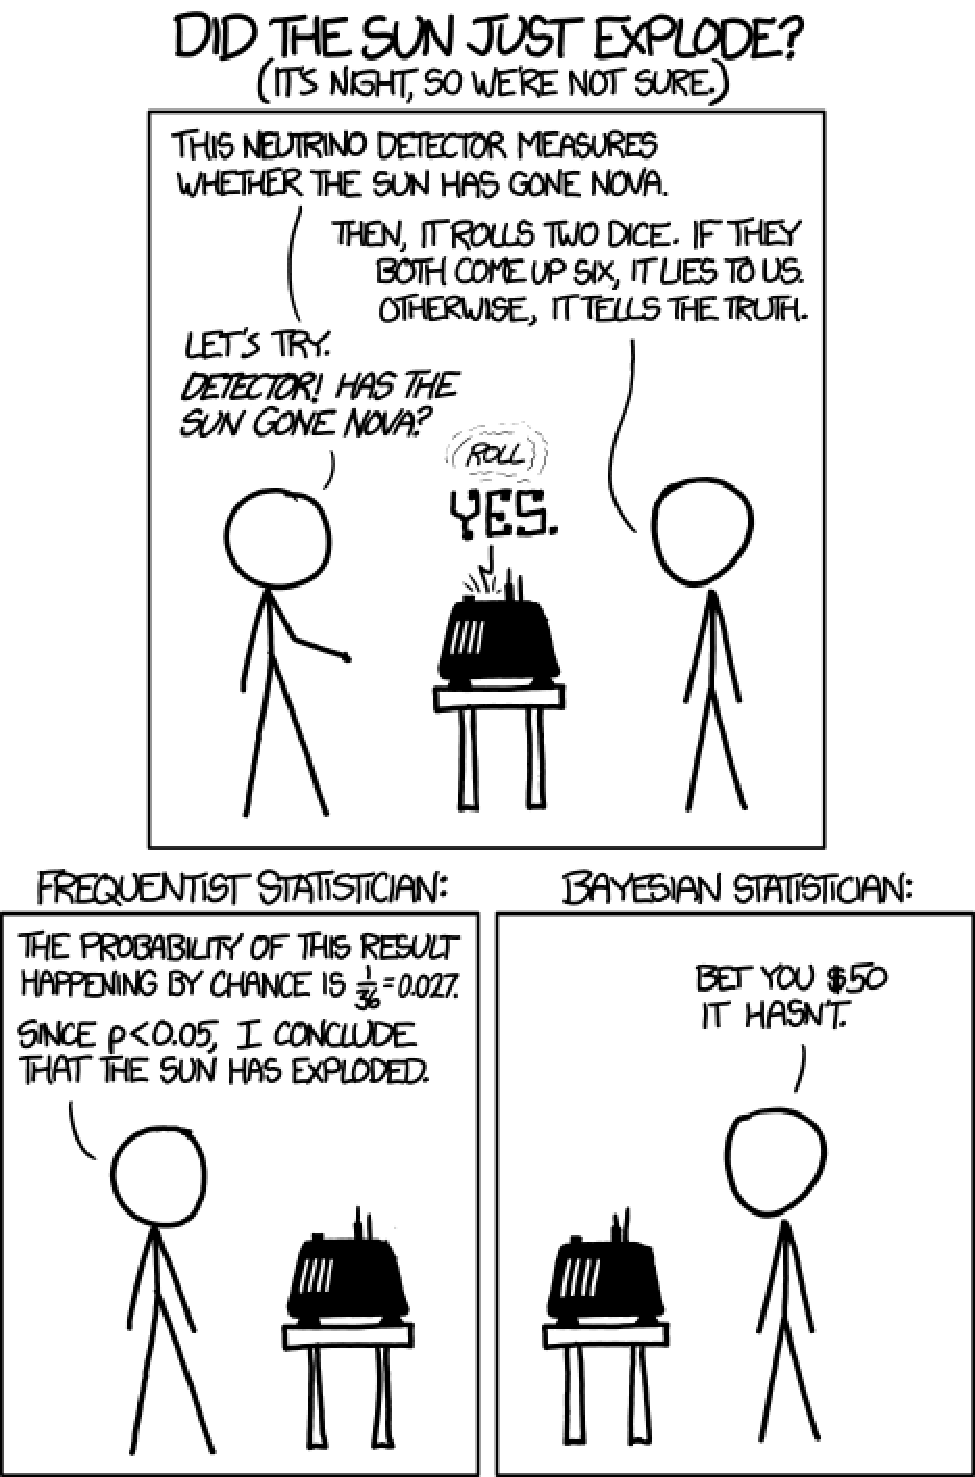
\includegraphics[width=8cm]{frequentists_vs_bayesians.pdf}

            \url{http://xkcd.com/1132/}, image publiée sous licence \href{http://xkcd.com/license.html}{CreativeCommons}.
\end{center}

Une chouette page concernant les intervalles de confiance à propos de l'élection à l'UMP est celle-ci :\\
\url{http://david.monniaux.free.fr/dotclear/index.php/post/2012/11/23/Le-sens-statistique-de-l-élection-à-l-UMP}

%+++++++++++++++++++++++++++++++++++++++++++++++++++++++++++++++++++++++++++++++++++++++++++++++++++++++++++++++++++++++++++ 
\section{Intervalle de fluctuation}
%+++++++++++++++++++++++++++++++++++++++++++++++++++++++++++++++++++++++++++++++++++++++++++++++++++++++++++++++++++++++++++

Cette section provient de \cite{JqcbOc}.

Un médecin voudrait savoir si le pourcentage d'habitants atteints d'hypertension artériel dans sa région est normal, sachant qu'une étude récemment publiée donne un pourcentage de \( 16\%\) pour d'autres régions comparables. Nous notons \( p\) la proportion (inconnue) d'hypertendus dans la région et nous constituons un échantillon de \( n=100\) habitants de la région. Nous notons \( f\) la fréquence des hypertendus dans l'échantillon.

Bien entendu, si la population est normale, le nombre \( f\) ne devrait pas être trop loin de \( 0.16\) -- à moins d'un coup de malchance dans la sélection de l'échantillon. Voyons cela de plus près.

Nous formulons l'hypothèse que la proportion des hypertendus est bien \( p=0.16\). Dans ce cas si nous désignons par \( X\) le nombre d'hypertendus dans l'échantillon, c'est une variable aléatoire binomiale de paramètres \( n=100\) et \( p=0.16\).

Toute la difficulté est évidemment maintenant de définir ce que nous appelons «normal». Pour donner une idée, voici les probabilités de la binomiale de paramètres \( n=100\), \( p=0.16\).

%The result is on figure \ref{LabelFigJRVlexw}. % From file JRVlexw
%\newcommand{\CaptionFigJRVlexw}{<+Type your caption here+>}
\begin{center}
\input{Fig_JRVlexw.pstricks}
\end{center}

La règle que nous allons retenir pour dire si une situation est «normale» est la suivante :
\begin{Aretenir}
    Une situation est «anormale» si elle a mois de \( 5\%\) de chance de s'expliquer par un coup de chance (ou de malchance, suivant le point de vue). Nous allons donc déclarer que les \( 2.5\%\) les plus à gauche et les \( 2.5\%\) les plus à droite sont anormaux.
\end{Aretenir}
Bien entendu dans le cas de notre médecin, avoir un nombre anormalement élevé de personnes en bonne santé n'est pas une \emph{mauvaise} nouvelle. 

Nous allons chercher des bornes \( a\) et \( b\) telles que \emph{au moins} \( 95\%\) des probabilités soient entre \( a\) et \( b\). Au niveau du dessin, ça donne ceci :


%The result is on figure \ref{LabelFigYVZAXhU}. % From file YVZAXhU
%\newcommand{\CaptionFigYVZAXhU}{<+Type your caption here+>}
\begin{center}
\input{Fig_YVZAXhU.pstricks}
\end{center}
Les zones rouges sont considérées comme anormales. En d'autres termes :
\begin{enumerate}
    \item
        Si sur l'échantillon de \( 100\) personnes prises dans la population le médecin observe \( 8\) ou moins sont atteintes d'hypertension, alors le médecin dira que sa région est en anormalement bonne santé. Il ne s'inquiétera pas, et ça fera un très bon thème de campagne de publicité pour les producteurs du fromage local.
    \item
        Si le nombre d'hypertendu est entre \( 9\) et \( 23\), le médecin dira qu'il n'y a rien de particulier à signaler.
    \item
        Si le nombre d'hypertendu est égal ou supérieur à \( 24\), alors la marque locale de fromage ne s'en vantera pas trop et le médecin essayera de comprendre ce qui ne fonctionne pas.
\end{enumerate}
L'intervalle entre \( 9\) et \( 23\) est nommé l'\defe{intervalle de fluctuation}{intervalle!fluctuation!de première}.

%+++++++++++++++++++++++++++++++++++++++++++++++++++++++++++++++++++++++++++++++++++++++++++++++++++++++++++++++++++++++++++ 
\section{Théorie}
%+++++++++++++++++++++++++++++++++++++++++++++++++++++++++++++++++++++++++++++++++++++++++++++++++++++++++++++++++++++++++++

Nous considérons une population dont une proportion \( p\)  présente un certain caractère, et nous prélevons (avec remise) un échantillon aléatoire de \( n\) personnes dans cette population. Nous notons \( X\) la variable aléatoire qui a pour valeur le nombre d'individus de l'échantillon présentant le caractère. Nous notons aussi \( f\) la fréquence d'observation du caractère dans l'échantillon.

La variable aléatoire \( X\) suit une loi binomiale de paramètres \( n\) et \( p\). 

Nous appelons \defe{intervalle de fluctuation}{intervalle!de fluctuation} à \( 95\%\) de la fréquence \( f\) l'intervalle 
\begin{equation}
    \left[ \frac{ a }{ n };\frac{ b }{ n } \right]
\end{equation}
où \(  a\) est le plus petit nombre tel que \( P(X\leq a)>0.025\) et \( b\) est le plus grand nombre tel que \( P(X\leq b)\geq 0.975\).

%+++++++++++++++++++++++++++++++++++++++++++++++++++++++++++++++++++++++++++++++++++++++++++++++++++++++++++++++++++++++++++ 
\section{Exemple}
%+++++++++++++++++++++++++++++++++++++++++++++++++++++++++++++++++++++++++++++++++++++++++++++++++++++++++++++++++++++++++++

La proportion de gauchers est de \( 12\%\).
\begin{enumerate}
    \item
        Combien de gauchers a-t-on dans la classe ?
    \item
        Est-ce que la proportion de gauchers dans la classe est «normale» ?
\end{enumerate}
Le fichier auquel on arrive est à peu près \info{gauchers.ods}.

\begin{Aretenir}
    La règle pour savoir quels sont les nombres à mettre dans l'intervalle de fluctuation est la suivante : il faut que \( P(X\leq a)=0.025\) et \( P(X\leq 0.95)\) soient tous les deux dans l'intervalle.
\end{Aretenir}


%&=& &=& &=& &=& &=& &=& &=& &=& &=& &=& &=& &=& &=& &=& &=& &=& &=& &=& &=& &=& &=& &=& &=& 
\part{Trucs pour les AP}
%&=& &=& &=& &=& &=& &=& &=& &=& &=& &=& &=& &=& &=& &=& &=& &=& &=& &=& &=& &=& &=& &=& &=& 
% This is part of Un soupçon de mathématique sans être agressif pour autant
% Copyright (c) 2014
%   Laurent Claessens
% See the file fdl-1.3.txt for copying conditions.

%+++++++++++++++++++++++++++++++++++++++++++++++++++++++++++++++++++++++++++++++++++++++++++++++++++++++++++++++++++++++++++ 
\section{Origami}
%+++++++++++++++++++++++++++++++++++++++++++++++++++++++++++++++++++++++++++++++++++++++++++++++++++++++++++++++++++++++++++

La feuille distribuée pour la découverte du théorème d'Haga.

% THÉORÈME DE HAGA POUR L'AP
\begin{feuilleExo}{Théorème de Haga}

%\begin{wrapfigure}{r}{10.cm}
    \begin{center}
\includegraphics[width=10cm]{Haga}
    \end{center}
%\end{wrapfigure}

\paragraph{Un peu de Pythagore}


Nous avons appelé \( a\) la longueur du segment \( [AC]\). Pourquoi \( BC=1-a\) ? Quelle est la valeur de \( a\) ?

\paragraph{Question d'angle}

Notons \( \hat B_1\) et \( \hat B_2\) les deux angles situés au point \( B\) (\( \hat B_1\) est celui du triangle \( ABC\)).
\begin{enumerate}
    \item
        Combien vaut \( \hat B_1+\hat B_2\) ?
    \item
        Combien vaut \( \hat B_1+\hat C\) ?
    \item
        En déduire que \( \hat B_2=\hat C\).
\end{enumerate}
Pourquoi \( \hat B_1=\hat E\) ?

\paragraph{Triangles semblables}

Les triangles \( ABC\) et \( BDE\) sont donc deux triangles ayant les mêmes angles; ils sont donc semblables et donc «proportionnels». De la même façon que pour Thalès, nous pouvons écrire les égalités «grand divisé par petit» :
\begin{equation}
    \frac{ DE }{ BD }=\frac{ AB }{ AC }.
\end{equation}
Reporter les valeurs connues et déduire la valeur de \( x=DE\).

\paragraph{Conclusion}

Sachant la valeur de \( x\), conclure que nous avons bien obtenu un pliage coupant en trois le côté du carré.

\end{feuilleExo}


Les diapositives projetées pour la présentation. 

\newpage
\subsection{Théorème de Haga (Pythagore)}

    \begin{multicols}{2}

    \begin{center}        
        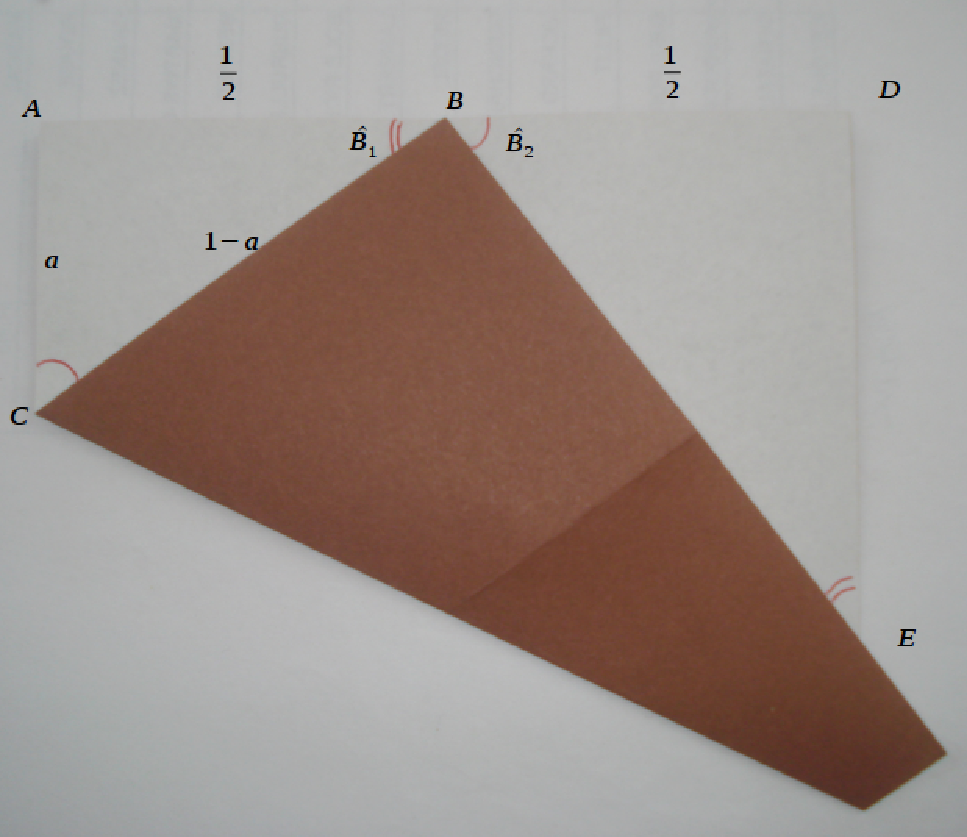
\includegraphics[width=5cm]{haga_coupe_anote}
    \end{center}


    Pythagore dans le triangle \( ABC\) : \( a^2+\left( \frac{ 1 }{2} \right)^2=(1-a)^2\).

    \( \Rightarrow \, a=\frac{ 3 }{ 8 }\).
    \end{multicols}

    
\newpage
\subsection{Théorème de Haga (angles)}
    \begin{multicols}{2}

    \begin{center}        
        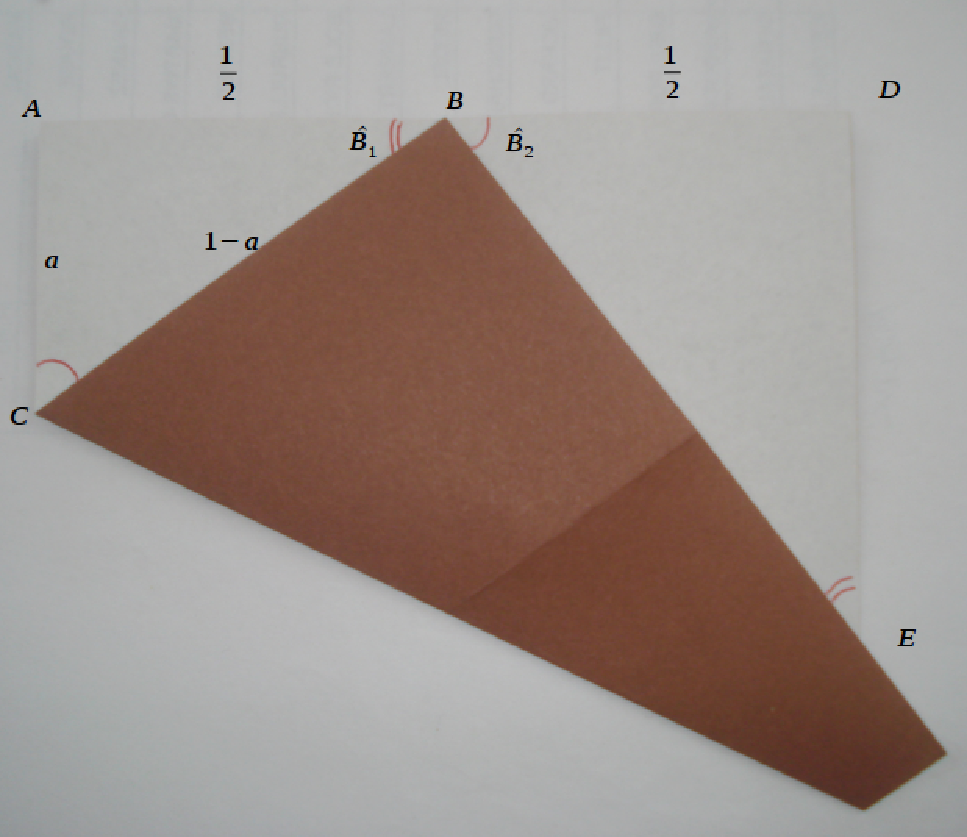
\includegraphics[width=5cm]{haga_coupe_anote}
    \end{center}

    \begin{subequations}
        \begin{numcases}{}
            \hat B_1+\hat B_2=90\\
            \hat B_1+\hat C=90\\
            \hat B_2+\hat E=90
        \end{numcases}
    \end{subequations}

    \( \Rightarrow \,   \hat B_2=\hat C \) et \( \hat B_1=\hat E\).
    \end{multicols}


    \begin{center}
        Les triangles \( ABC\) et \( BDE\) sont semblables.
    \end{center}

\newpage
\subsection{Théorème de Haga (proportionnalité)}
    \begin{multicols}{2}

    \begin{center}        
        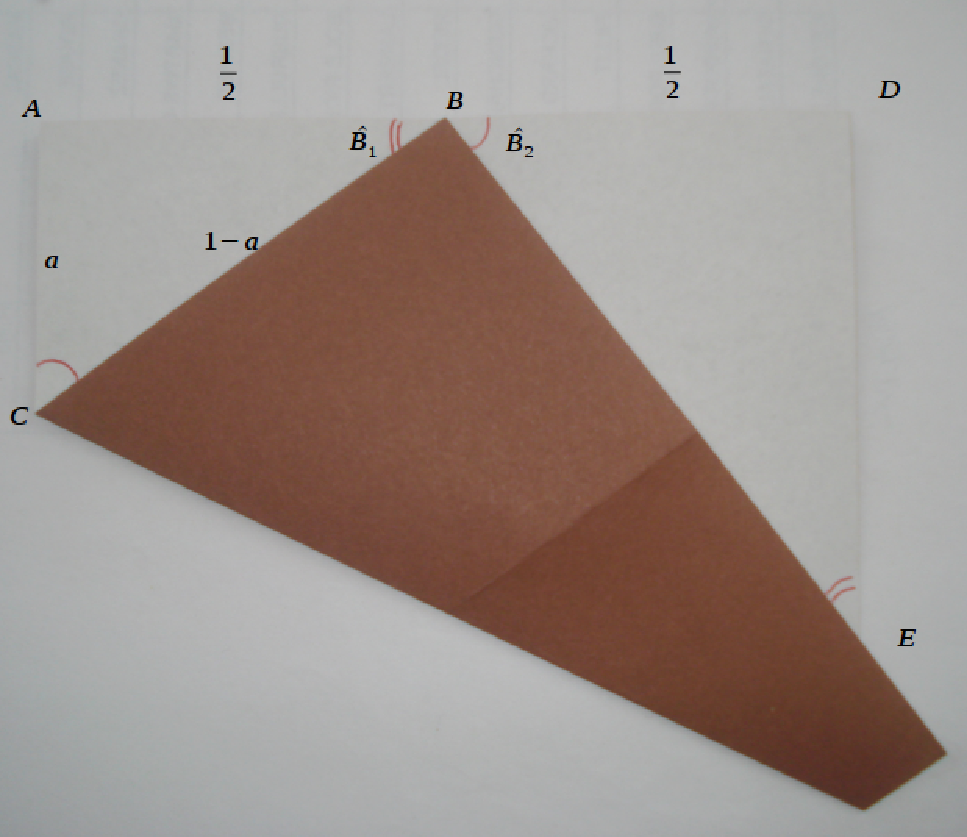
\includegraphics[width=5cm]{haga_coupe_anote}
    \end{center}

    \begin{equation}
        \frac{ DE }{ AB }=\frac{ BD }{ AC }
    \end{equation}
    \begin{equation}
        \frac{ DE }{ \frac{ 1 }{2} }=\frac{ \frac{ 1 }{2} }{ \frac{ 3 }{ 8 } }
    \end{equation}
    \begin{equation}
        2DE=\frac{ 4 }{ 3 }
    \end{equation}
    \begin{equation}
        DE=\frac{2}{ 3 }.
    \end{equation}
    \end{multicols}


%&=& &=& &=& &=& &=& &=& &=& &=& &=& &=& &=& &=& &=& &=& &=& &=& &=& &=& &=& &=& &=& &=& &=& 
\part{Python}
%&=& &=& &=& &=& &=& &=& &=& &=& &=& &=& &=& &=& &=& &=& &=& &=& &=& &=& &=& &=& &=& &=& &=& 
% This is part of Un soupçon de mathématique sans être agressif pour autant
% Copyright (c) 2012
%   Laurent Claessens
% See the file fdl-1.3.txt for copying conditions.

\chapter{Structures de base}

\begin{remark}
    Certains bouts de codes donnés ici commencent par la ligne
    \begin{quote}
        \info{\# -*- coding: utf8 -*-}
    \end{quote}
    Si vous savez ce que signifie «\wikipedia{fr}{Utf8}{utf8}», vous devriez deviner à quoi sert cette ligne. Sinon c'est pas grave : vous n'êtes pas \emph{obligés} de l'écrire dans vos programmes, mais c'est une bonne habitude à prendre. Nous en reparlerons peut-être plus tard.
\end{remark}

%---------------------------------------------------------------------------------------------------------------------------
\subsection{La fonction \info{print}}
%---------------------------------------------------------------------------------------------------------------------------

Python ne prend pas d'initiatives. Si vous ne lui demandez pas d'écrire quelque chose, il n'écrira rien. La commande la plus courante\footnote{Bien entendu, python permet de programmer des fenêtres, des boutons et autres boites de dialogue, auquel cas ce ne sera plus la commande \info{print} qui jouera.} pour afficher quelque chose à l'écran est la commande \info{print}. 
\begin{enumerate}
    \item
        Pour afficher la valeur d'une variable \info{a}, mettre \info{print(a)}.
    \item
        Pour afficher un texte (par exemple «bonjour» ), mettre des guillemets : \info{print(``bonjour'')}.
\end{enumerate}
Si vous voulez afficher plusieurs choses, vous les séparez par une virgule.

\lstinputlisting{ex_print.py}

donne

\lstinputlisting[title=Résultat]{res_ex_print.txt}

Notez que les lignes qui commencent par \# ne sont pas prises en compte. Cela permet au programmeur de mettre des notes pour lui-même. N'hésitez pas à en mettre pour rendre votre code plus lisible.

\Exo{Premiere-0037}

%+++++++++++++++++++++++++++++++++++++++++++++++++++++++++++++++++++++++++++++++++++++++++++++++++++++++++++++++++++++++++++
\section{Listes}
%+++++++++++++++++++++++++++++++++++++++++++++++++++++++++++++++++++++++++++++++++++++++++++++++++++++++++++++++++++++++++++

Une liste est une collection ordonnée d'éléments. Elle se définit avec des crochets.

\lstinputlisting{ex_listes.py}

donne

\lstinputlisting[title=Résultat]{res_ex_listes.txt}

Nous pouvons ajouter un élément à une liste en utilisant la \emph{méthode} \info{append}, et retrouver un élément d'une liste par son numéro (attention : python numérote à partie de zéro), en demandant par exemple \info{A[4]} pour l'élément numéro \( 4\) de la liste \info{A}. Cela sera donc le cinquième élément de la liste. Cas spécial : le dernier élément de la liste est le numéro \( -1\).

\lstinputlisting{ex_listes2.py}

donne

\lstinputlisting[title=Résultat]{res_ex_listes2.txt}


\Exo{Premiere-0033}


La multiplication d'une liste par un nombre donne la liste contenant plusieurs fois la liste originale. Nous ajoutons une liste à une autre en utilisant la méthode \info{extend}.


\lstinputlisting{ex_listes3.py}

donne

\lstinputlisting[title=Résultat]{res_ex_listes3.txt}


\Exo{Premiere-0034}

%+++++++++++++++++++++++++++++++++++++++++++++++++++++++++++++++++++++++++++++++++++++++++++++++++++++++++++++++++++++++++++
\section{Quelque mots à propos des fonctions}
%+++++++++++++++++++++++++++++++++++++++++++++++++++++++++++++++++++++++++++++++++++++++++++++++++++++++++++++++++++++++++++

%---------------------------------------------------------------------------------------------------------------------------
\subsection{Choses Basiques}
%---------------------------------------------------------------------------------------------------------------------------

Si un calcul doit être refait plusieurs fois dans un même programme, il est bon d'écrire une fonction qui sera appelée à chaque fois. En python, une fonction se déclare avec le mot-clef \info{def} comme ceci :
\begin{quote}
    \info{def\ nom\_de\_ma\_fonction(a,b):}
\end{quote}
où \info{a} et \info{b} seront les arguments de la fonction. Il peut y en avoir un seul, deux, ou plus (pas de limites), ou pas du tout. Une fonction peut afficher et calculer autant de résultats intermédiaires que l'on veut. 

\lstinputlisting{ex_fonction.py}

donne

\lstinputlisting[title=Résultat]{res_ex_fonction.txt}

Cette fonction ne fait qu'afficher du texte, mais ne retourne pas de valeurs. Voici une fonction qui retourne \( 1\) si le nombre donné est plus grand ou égal à zéro et retourne \( -1\) si il est négatif.


\lstinputlisting{ex_fonction2.py}

donne

\lstinputlisting[title=Résultat]{res_ex_fonction2.txt}


\Exo{Premiere-0066}


\Exo{Premiere-0068}

%---------------------------------------------------------------------------------------------------------------------------
\subsection{Pour aller plus loin}
%---------------------------------------------------------------------------------------------------------------------------

La fonction de l'exemple précédent peut être simplifiée en sachant que dès que une instruction \info{return} est rencontrée, l'exécution de la fonction est \emph{immédiatement} stoppée et la valeur est retournée. Nous pouvons donc écrire

\lstinputlisting{ex_fonction3.py}

Si le nombre donné est positif, un \info{return} est rencontré à l'intérieur du \info{if}, et l'autre \info{return} n'est jamais rencontré.

D'autre part, une fonction peut vraiment prendre \emph{n'importe quoi} comme argument, y compris des autres fonctions. Dans l'exemple suivant, la fonction \info{evaluation} prend un argument une fonction et un nombre, et retourne la fonction évaluée en ce nombre.

\lstinputlisting{ex_fonction4.py}

donne

\lstinputlisting[title=Résultat]{res_ex_fonction4.txt}

%+++++++++++++++++++++++++++++++++++++++++++++++++++++++++++++++++++++++++++++++++++++++++++++++++++++++++++++++++++++++++++
\section{Télécharger automatiquement une liste de liens}
%+++++++++++++++++++++++++++++++++++++++++++++++++++++++++++++++++++++++++++++++++++++++++++++++++++++++++++++++++++++++++++

Nous allons maintenant utiliser nos connaissances pour résoudre un problème pratique : comment télécharger automatiquement une série de liens sans devoir cliquer des milliers de fois sur le bouton droit et «enregistrer sous» ?

%+++++++++++++++++++++++++++++++++++++++++++++++++++++++++++++++++++++++++++++++++++++++++++++++++++++++++++++++++++++++++++
\section{Tester la divisibilité}
%+++++++++++++++++++++++++++++++++++++++++++++++++++++++++++++++++++++++++++++++++++++++++++++++++++++++++++++++++++++++++++

Nous aurons de temps en temps besoin de tester si un nombre est divisible par deux, par trois ou par autre chose.

Testez le programme suivant.

\lstinputlisting{ex_division.py}

Est-ce que vous pouvez en déduire un critère de divisibilité basé sur l'usage de la «division entière» \info{\%} ? Regardez combien vaut \info{i\%4} pour les \info{i} qui sont divisible par \( 4\).

\Exo{Premiere-0067}

%+++++++++++++++++++++++++++++++++++++++++++++++++++++++++++++++++++++++++++++++++++++++++++++++++++++++++++++++++++++++++++
\section{Moyenne, médiane, quartiles}
%+++++++++++++++++++++++++++++++++++++++++++++++++++++++++++++++++++++++++++++++++++++++++++++++++++++++++++++++++++++++++++
\label{SecZYftar}

%---------------------------------------------------------------------------------------------------------------------------
\subsection{Moyenne}
%---------------------------------------------------------------------------------------------------------------------------

\begin{example}     \label{ExerfDMnv}
    % Note : la liste ci-dessous est codée en dur dans les scripts d'exemples. Si on la modifie, il faut modifier les scripts.
    Un magasin de chaussures a vendu des tailles entre \( 40\) et \( 45\) suivant la distribution suivante :
    \begin{center}
        \begin{tabular}{|l||c|c|c|c|c|c|}
            \hline
            taille \( x_i\)&40&41&42&43&44&45\\
            \hline
            effectifs \( n_i\)&3&5&10&8&2&4\\
            \hline
        \end{tabular}
    \end{center}
    Nous voudrions calculer la moyenne, la médiane et les quartiles de la distribution des tailles de chaussures. Nous allons nous occuper de cela dans les pages qui viennent.
\end{example}
    
    Pour calculer la moyenne d'une liste, nous devons savoir la longueur et la somme de ses éléments. Python fournit cela assez rapidement. Si \info{A} est une liste,
    \begin{enumerate}
        \item
            \info{len(A)} est la longueur de \info{A},
        \item
            \info{sum(A)} est la somme de ses éléments.
    \end{enumerate}
    
\Exo{Premiere-0035}
%---------------------------------------------------------------------------------------------------------------------------
\subsection{Premier et troisième quartiles}
%---------------------------------------------------------------------------------------------------------------------------

Pour les quartiles, nous nous rappelons que si \( n\) est le nombre de valeurs, alors le rang du premier quartile est le premier entier supérieur à \( n/4\); et le rang du troisième quartile est le premier entier supérieur à \( 3n/4\). Par exemple si il y a \( 15\) données, nous calculons \( 3\times 15/3= 11.25\), et le troisième quartile sera la douzième valeur.


Bien entendu python possède une commande qui retourne le premier entier supérieur à un nombre donné. C'est la commande \info{ceil} du module \info{math}. En pratique :

\lstinputlisting{exemple_ceil.py}

donne 

\lstinputlisting{res_exemple_ceil.txt}
De même la fonction \info{math.floor} retourne le premier entier inférieur à un nombre donné. Par exemple \info{math.floor(3.89)} vaut \( 3\).

La ligne \info{import math} s'appelle «importer le module math», et nous n'en dirons sans doute pas plus sur la notion d'import de module. Le module \info{math} contient encore de nombreuses fonctions mathématiques qui transforment python en une très puissante\footnote{Pour donner une idée, la mémoire disponible sur des calculatrices modernes est à peu près la même que celle qui était disponible sur Apple II au début des années 1980; avec python vous pouvez exploiter toute la mémoire de votre ordinateur, ou de votre téléphone ou de votre tablette ou de quoi que ce soit sur lequel vous avez python.} calculatrice scientifique.


\Exo{Premiere-0036}

\Exo{Premiere-0038}

%+++++++++++++++++++++++++++++++++++++++++++++++++++++++++++++++++++++++++++++++++++++++++++++++++++++++++++++++++++++++++++
\section{La boucle \info{for}}
%+++++++++++++++++++++++++++++++++++++++++++++++++++++++++++++++++++++++++++++++++++++++++++++++++++++++++++++++++++++++++++

Il est possible de répéter une action pour tous les éléments d'une liste. Par exemple

\lstinputlisting{ex_for1.py}

La première boucle écrit \info{x} et son carré pour tout \info{x} dans la liste \info{[1,5,10,2]}. La seconde boucle écrit tous les lettres du mot «bonjour» et la troisième tous les nombres dans \info{range(0,5)}, c'est à dire \( 0\), \( 1\), \( 2\), \( 3\) et \( 4\).

\lstinputlisting[title=Résultat]{res_ex_for1.txt}

\Exo{Premiere-0048}

%+++++++++++++++++++++++++++++++++++++++++++++++++++++++++++++++++++++++++++++++++++++++++++++++++++++++++++++++++++++++++++
\section{Prendre des choses au hasard}
%+++++++++++++++++++++++++++++++++++++++++++++++++++++++++++++++++++++++++++++++++++++++++++++++++++++++++++++++++++++++++++

Python permet de tirer des nombres au hasard ou de prendre un élément au hasard dans une liste ou dans un texte. Pour cela il y a le module \info{random}. Si \info{A} est une liste ou un texte (chaîne de caractère), alors
\begin{quote}
    \info{random.choice(A)}
\end{quote}
retourne un élément au hasard de la suite.

\Exo{Premiere-0049}
\Exo{Premiere-0050}

\chapter{Suite définie par récurrence}

Soit une suite définie par récurrence

\begin{subequations}
    \begin{numcases}{}
    u_0=10\\
    u_{n+1}=2u_n.
    \end{numcases}
\end{subequations}

Nous voudrions pouvoir répondre à plusieurs types de questions :
\begin{enumerate}
    \item
        construire une liste contenant les \( 100\) premiers termes de la suite;
    \item
        savoir quel est le premier terme à dépasser un million.
    \item
        Quelle est l'allure générale de la suite ? Croissante ? Décroissante ?
\end{enumerate}

Avant de se lancer, nous devons nous poser une question de vocabulaire : est-ce que le centième terme de la suite \( u\) est \( u_{100}\) ou \( u_{99}\) ? Le premier terme étant \( u_0\), le centième est bien \( u_{99}\).


\Exo{Premiere-0056}

\lstinputlisting{recurrence1.py}

donne

\lstinputlisting{res_recurrence1.txt}

Notons que la ligne \info{print(u[100])} plante avec l'erreur \info{list index out of range}, c'est à dire que la liste \info{u} n'a pas d'élément \info{u[100]}, ce qui est normal parce qu'elle contient \( 100\) éléments et que la numérotation commence à zéro.


\Exo{Premiere-0039}


    En pratique, sachez que pour savoir le plus grand élément d'une liste, python dispose de la fonction \info{max}. Pour la suite, utilisez cette dernière, et non cette que vous aurez programmé dans cet exercice.


\Exo{Premiere-0057}

En ce qui concerne la possibilité de trouver le premier élément qui dépasse le million, le programme suivant donne une manière d'aborder le problème.

\lstinputlisting{recurrence2.py}

donne

\lstinputlisting{res_recurrence2.txt}

\Exo{Premiere-0058}

\begin{remark}
    
    Le code donné dans le programme \info{recurrence2.py} (cf. plus haut) donne \( 17\) et celui de l'exercice \ref{exoPremiere-0058} donne donne \( 18\). Qui a raison ? Le \( 18\) de la seconde méthode est la longueur de la liste construite, donc il indique que le premier terme à passer le million est \( u_{17}\) (vu que le premier terme est \( u_0\), la longueur est toujours un plus grande que le numéro du dernier élément).

La réponse est donc que \( u_{17}\) est le premier élément à être plus grand que un million, mais \( u_{17}\) est le dix-huitième élément de la liste.

\end{remark}

\Exo{Premiere-0055}

\chapter{Manipulation de texte}

%+++++++++++++++++++++++++++++++++++++++++++++++++++++++++++++++++++++++++++++++++++++++++++++++++++++++++++++++++++++++++++
\section{Manipulation de base}
%+++++++++++++++++++++++++++++++++++++++++++++++++++++++++++++++++++++++++++++++++++++++++++++++++++++++++++++++++++++++++++

Pour mettre un texte dans une variable, il suffit de le faire :

\lstinputlisting{ex_texte1.py}
donne
\lstinputlisting[title=Résultat]{res_ex_texte1.txt}

Les chaînes de caractères (par exemple la variable \info{a} de l'exemple) peuvent être utilisées comme des listes. Il est possible d'en demander des parties.

\lstinputlisting{ex_texte2.py}
donne
\lstinputlisting[title=Résultat]{res_ex_texte2.txt}

La longueur d'un texte est donnée par \info{len(a)}.

Nous pouvons un peu automatiser :
\lstinputlisting{ex_texte3.py}
donne
\lstinputlisting[title=Résultat]{res_ex_texte3.txt}

%+++++++++++++++++++++++++++++++++++++++++++++++++++++++++++++++++++++++++++++++++++++++++++++++++++++++++++++++++++++++++++
\section{Passer des textes aux listes et inversement}
%+++++++++++++++++++++++++++++++++++++++++++++++++++++++++++++++++++++++++++++++++++++++++++++++++++++++++++++++++++++++++++

Si nous avons une suite de lettres, il est possible de la transformer en texte (chaîne de caractères), et inversement. Si \info{texte} est une chaîne de caractères, alors
\begin{quote}
    \info{list(A)}
\end{quote}
est la liste de ses caractères. La conversion dans ce sens est d'un intérêt limité parce que le gros des fonctionnalités des listes sont accessibles aux chaînes de caractères.

La conversion d'une liste en une chaîne est plus intéressante parce qu'elle permet de créer un texte «petit bout par petit bout». La méthode est la suivante. Si \info{A} est une liste alors
\begin{quote}
    \info{``''.join(A)}
\end{quote}
est la chaîne correspondante. Mieux : 
\begin{quote}
    \info{``-''.join(A)}
\end{quote}
est un texte qui «joint» les éléments de \info{A} par des tirets.


\Exo{Premiere-0070}

\lstinputlisting{ex_join1.py}

donne

\lstinputlisting[title=Résultat]{res_ex_join1.txt}


\Exo{Premiere-0051}

Il y a encore mieux. Il faut savoir que la chaîne \info{``\textbackslash n''} représente un saut de ligne. Par conséquent, en reliant les éléments d'une liste par un \info{``\textbackslash n''}, nous pouvons écrire les éléments en colonne. 

\lstinputlisting{ex_join2.py}

donne

\lstinputlisting[title=Résultat]{res_ex_join2.txt}

Et enfin, une dernière conversion consiste à séparer un texte en élément séparés par une chaîne. 

\lstinputlisting{ex_split1.py}

donne

\lstinputlisting[title=Résultat]{res_ex_split1.txt}


\Exo{Premiere-0052}

%+++++++++++++++++++++++++++++++++++++++++++++++++++++++++++++++++++++++++++++++++++++++++++++++++++++++++++++++++++++++++++
\section{Un texte qui ressemble à du français}
%+++++++++++++++++++++++++++++++++++++++++++++++++++++++++++++++++++++++++++++++++++++++++++++++++++++++++++++++++++++++++++

L'analyse de la fréquence des lettres dans un texte permet aussi de détecter la langue. Regardons ces trois textes, classés par ordre croissant de «crédibilité»:

\begin{quote}
    uuerlh i,ie oceieomriosnuu éctes 'qD umixnohpsnaedoteirinmrpouont nqenc a ltvpa n gcudttn  sercacuqe bu'iido retsaiacean sat oc leiu n  eéiteMe e   t  rtlteu rdédndame giaeosmx'raeaeea  jo m uds tum   et uaecetrûauu leel ttoœaxergs m'u aq uea un ileetid 'n utztotee isiranit aar,s evd e emlt zreumaganai nm,tlren id ouna,àadg lvnu s ai ie sut oqtrnœ u'nvtaoiemooe l  dqar meecésnc  jruscuttmse Aaasee ede netps  e riih
\end{quote}
Ce premier texte a été généré en prenant des lettres (y compris les espaces) au hasard dans un texte de référence\footnote{En l'occurence, \emph{Le temps retrouvé}.}. La fréquence des lettres est donc la même (aux aléas statistiques près) que la fréquence en français, mais force est d'avouer que cela ne ressemble pas tellement à du vrai français.
%TODO : mettre un lien vers wikisource pour le temps retrouvé
 
Second extrait :
\begin{quote}
    aiffe ditet ntta t cos rape uelloux sss éstére dile dsiten pen douitese Mmbis é ai quder ndises gau r qul aure à arsois arons à avese durcet l'Ountai vountel'aue i seuneueras e de beucene, la à qutout prmmontuxtri cet, rès ppllall anért me lle nte me s qujascoun c'œidisquss tintouvens me à nolllqut quiepomatrèraitra de meps fefr ll'ers'œusue suont de d ventistétapamer condes
\end{quote}
Cela est déjà un peu mieux. Notez en particulier la longueur des mots qui est plus raisonnable que dans le premier extrait. Voici comment il a été créé.
\begin{enumerate}
    \item
        La première lettre est tirée au hasard dans l'alphabet. Ici ça a été un «a».
    \item
        Nous cherchons tous les «a» dans le texte de référence, nous en prenons un au hasard, et nous ajoutons au texte la lettre \emph{qui suit}. Ici ça a été un «i». 
    \item
        Nous cherchons tous les «i» dans le texte de référence, etc.
\end{enumerate}
Cela explique pourquoi dans l'extrait donné, tous les «q» sont suivis d'un «u». En effet, dans le texte de référence presque tous les «q» sont suivis d'un «u». D'ailleurs, connaissez-vous un mot en français contenant un «q» non suivit d'un «u» ? Notez aussi qu'il y a six double «l», un seul double «m» et aucun double «e». Cela s'explique assez facilement en connaissant le français.

\begin{remark}
Dans le texte de référence, il y a des «q» non suivis de «u» dans les mots «piqûre», «coq», «cinq» (il est alors suivit d'un espace). La chaîne «qu» arrive 13528 fois dans le texte de référence et «q» suivit d'autre chose que «u» arrive seulement 24 fois.
\end{remark}

Troisième extrait :
\begin{quote}
Epgues vu un peut en m'avaisansfortes pour le dans que tout, cands ces cela comptableure amours dantestre ver aurais avaites, dont son de pours le simultés des planter, paysalutant évidue leux qu'ailles touffirer, ajour même un combianchez lui on de cholont décrir. Commette était même fortueux et de paru avait que jours pitait nulleurir cette le ce montions, nouvaien plaissé que sespèce souvoir connemi les gens ou resse solais ans mant ent, il du n'y a rançait au se dois « Alpe trientaient de Guer
\end{quote}
De loin, cela ressemble presque à s'y méprendre à du français, mais de près, on remarque que presque aucun mot n'est correct bien que tous les mots soient prononçables. Ce dernier extrait fut composé de la façon suivante.

\begin{enumerate}
    \item
        Choisir 3 lettres au hasard. Ici «epg» 
    \item
        Chercher tous les «epg» dans le texte de référence, et ajouter à l'extrait la lettre suivante. Ici c'est un «u» qui est ajouté.
    \item
        Chercher tous les «pgu» etc.
\end{enumerate}

Nous allons tenter de récrire un programme qui donne cet effet.


Un dernier pour la route. Exactement le même programme, mais en prenant un roman de Sherlock Holmes (en anglais) comme texte de référence.
\begin{quote}
dèWatseculiance is marked, at taken the unlikely siden would he placed man why Who becall wife you be othe for For to that the Amering raised. Thing his feely. "'Thand she sodes get wond infety. I said who which show will details. In see, and the Alic slansper, for stonvicturnia, and Lest but, 1892 "Shile, Petel. Then, and to man it und in my chan aframa. My litter gretaring me entagementyfound gent that, 1892 "Well days dramongroofs when some the looks upon pa weeks a reason a pipe of Penting wif
\end{quote}
Cela ressemble à de l'anglais sans aucun doute.

\Exo{Premiere-0053}
\Exo{Premiere-0054}

%+++++++++++++++++++++++++++++++++++++++++++++++++++++++++++++++++++++++++++++++++++++++++++++++++++++++++++++++++++++++++++
\section{Exercices}
%+++++++++++++++++++++++++++++++++++++++++++++++++++++++++++++++++++++++++++++++++++++++++++++++++++++++++++++++++++++++++++

\Exo{Premiere-0027}



\part{Exercices}


\chapter{Autres exercices}
%+++++++++++++++++++++++++++++++++++++++++++++++++++++++++++++++++++++++++++++++++++++++++++++++++++++++++++++++++++++++++++ 
\section{Repères}
%+++++++++++++++++++++++++++++++++++++++++++++++++++++++++++++++++++++++++++++++++++++++++++++++++++++++++++++++++++++++++++

%\Exo{Seconde-0002}         % Celui-ci est enlevé parce qu'il est inséré au cours.
\Exo{smath-0479}
\Exo{smath-0021}
\Exo{smath-0028}
\Exo{Seconde-0100}
\Exo{Seconde-0085}
\Exo{Seconde-0083}
\Exo{Seconde-0003}
\Exo{Seconde-0084}
\Exo{Seconde-0099}
\Exo{Seconde-0013}
\Exo{Seconde-0021}
\Exo{Seconde-0079}
\Exo{Seconde-0080}
\Exo{Seconde-0078}
\Exo{smath-0029}
\Exo{Seconde-0081}
\Exo{Seconde-0077}
\Exo{smath-0027}
\Exo{Seconde-0082}
\Exo{Seconde-0001}
\Exo{Seconde-0062}
\Exo{smath-0026}
\Exo{smath-0515}

%+++++++++++++++++++++++++++++++++++++++++++++++++++++++++++++++++++++++++++++++++++++++++++++++++++++++++++++++++++++++++++ 
\section{Fonctions affines}
%+++++++++++++++++++++++++++++++++++++++++++++++++++++++++++++++++++++++++++++++++++++++++++++++++++++++++++++++++++++++++++

%--------------------------------------------------------------------------------------------------------------------------- 
\subsection{Équations de droites}
%---------------------------------------------------------------------------------------------------------------------------

\Exo{smath-0413}
\Exo{smath-0154}
\Exo{smath-0330}        % Cet exo est le même que le smath-155, mais en plus court pour rentrer dans un devoir.
\Exo{smath-0344}
\Exo{smath-0128}
\Exo{smath-0409}    % presque le même que le smath-0149, mais plus court pour un DS.
\Exo{smath-0130}
\Exo{smath-0069}
\Exo{smath-0394}
\Exo{smath-0229}    % Le même que smath-0413, mais en plus guidé pour un DS.
\Exo{smath-0150}    
\Exo{smath-0155}
\Exo{smath-0151}
\Exo{smath-0086}
\Exo{smath-0138}
\Exo{smath-0200}
\Exo{smath-0233}
\Exo{smath-0234}
\Exo{smath-0153}
\Exo{Seconde-0019}

%--------------------------------------------------------------------------------------------------------------------------- 
\subsection{Tableaux de variation et de signe}
%---------------------------------------------------------------------------------------------------------------------------

\Exo{smath-0132}
\Exo{smath-0321}

%---------------------------------------------------------------------------------------------------------------------------
\subsection{Parallélisme et intersection}
%---------------------------------------------------------------------------------------------------------------------------

%TODO : écrire un exercice avec un rebond sur une table de billard.
\Exo{smath-0083}
\Exo{smath-0129}
\Exo{smath-0110}    % TODO: il faut plus d'exercices comme celui-ci.
\Exo{smath-0084}

\Exo{smath-0235}
\Exo{smath-0236}
\Exo{smath-0237}
\Exo{smath-0239}
\Exo{smath-0345}
\Exo{smath-0451}
\Exo{smath-0450}


%--------------------------------------------------------------------------------------------------------------------------- 
\subsection{Problèmes}
%---------------------------------------------------------------------------------------------------------------------------

\Exo{smath-0241}
\Exo{smath-0242}

%+++++++++++++++++++++++++++++++++++++++++++++++++++++++++++++++++++++++++++++++++++++++++++++++++++++++++++++++++++++++++++ 
\section{Fonctions et résolutions}
%+++++++++++++++++++++++++++++++++++++++++++++++++++++++++++++++++++++++++++++++++++++++++++++++++++++++++++++++++++++++++++

%---------------------------------------------------------------------------------------------------------------------------
\subsection{Image, antécédent}
%---------------------------------------------------------------------------------------------------------------------------

\Exo{smath-0516}
\Exo{Seconde-0042}
\Exo{Seconde-0048}
\Exo{Seconde-0054}
\Exo{Seconde-0051}
\Exo{Seconde-0050}

%---------------------------------------------------------------------------------------------------------------------------
\subsection{Exemples de fonctions}
%---------------------------------------------------------------------------------------------------------------------------

\Exo{Seconde-0058}
\Exo{Seconde-0057}
\Exo{Seconde-0063}
\Exo{Seconde-0061}
\Exo{Seconde-0067}
\Exo{smath-0295}

\Exo{Seconde-0071}
\Exo{smath-0015}
\Exo{smath-0210}
\Exo{smath-0004}
\Exo{smath-0005}
\Exo{smath-0006}
\Exo{Seconde-0046}

\Exo{smath-0186}    % Cet exercice est le même que le smath-0111, mais vu différemment.
\Exo{smath-0078}
\Exo{smath-0013}
\Exo{Seconde-0068}
\Exo{Seconde-0064}
\Exo{Seconde-0044}
\Exo{Seconde-0066}
\Exo{Seconde-0076}
\Exo{Seconde-0059}
\Exo{Seconde-0060}
%---------------------------------------------------------------------------------------------------------------------------
\subsection{Plus avancés}
%---------------------------------------------------------------------------------------------------------------------------

\Exo{Premiere-0018}

%+++++++++++++++++++++++++++++++++++++++++++++++++++++++++++++++++++++++++++++++++++++++++++++++++++++++++++++++++++++++++++ 
\section{Comparaison de séries statistiques}
%+++++++++++++++++++++++++++++++++++++++++++++++++++++++++++++++++++++++++++++++++++++++++++++++++++++++++++++++++++++++++++

\Exo{smath-0378}
\Exo{smath-0243}
\Exo{smath-0244}
\Exo{smath-0245}
\Exo{smath-0246}
\Exo{smath-0247}
\Exo{smath-0248}
\Exo{smath-0249}
\Exo{smath-0216}
\Exo{smath-0392}

%+++++++++++++++++++++++++++++++++++++++++++++++++++++++++++++++++++++++++++++++++++++++++++++++++++++++++++++++++++++++++++ 
\section{La fonction carré}
%+++++++++++++++++++++++++++++++++++++++++++++++++++++++++++++++++++++++++++++++++++++++++++++++++++++++++++++++++++++++++++

\Exo{smath-0176}
\Exo{smath-0178}
\Exo{smath-0252}
\Exo{smath-0179}
\Exo{smath-0177}
\Exo{smath-0141}
\Exo{smath-0254}
\Exo{smath-0139}
\Exo{smath-0180}
\Exo{smath-0140}
\Exo{smath-0174}
\Exo{smath-0175}
\Exo{smath-0253}
\Exo{smath-0255}
\Exo{smath-0266}

%+++++++++++++++++++++++++++++++++++++++++++++++++++++++++++++++++++++++++++++++++++++++++++++++++++++++++++++++++++++++++++ 
\section{Fonctions homographiques}
%+++++++++++++++++++++++++++++++++++++++++++++++++++++++++++++++++++++++++++++++++++++++++++++++++++++++++++++++++++++++++++

\Exo{smath-0334}
\Exo{smath-0379}
\Exo{smath-0368}
\Exo{smath-0137}
\Exo{smath-0144}
\Exo{smath-0316}
\Exo{smath-0335}
\Exo{smath-0336}
\Exo{smath-0377}

%+++++++++++++++++++++++++++++++++++++++++++++++++++++++++++++++++++++++++++++++++++++++++++++++++++++++++++++++++++++++++++ 
\section{Fonction inverse}
%+++++++++++++++++++++++++++++++++++++++++++++++++++++++++++++++++++++++++++++++++++++++++++++++++++++++++++++++++++++++++++

% Il faut un peu reclasser ces exercices.

\Exo{smath-0262}
\Exo{smath-0257}
\Exo{smath-0258}

\Exo{smath-0369}
\Exo{smath-0350}
\Exo{smath-0276}
\Exo{smath-0260}
\Exo{smath-0259}
\Exo{smath-0261}
\Exo{smath-0265}
\Exo{smath-0268}
\Exo{smath-0272}
\Exo{smath-0273}
\Exo{smath-0274} 
\Exo{smath-0275}
\Exo{smath-0277}
\Exo{smath-0278}
\Exo{smath-0292}
\Exo{smath-0294}
\Exo{smath-0346}
\Exo{smath-0364}
\Exo{smath-0256}        % Cet exercice n'apporte rien.
\Exo{smath-0406}

%+++++++++++++++++++++++++++++++++++++++++++++++++++++++++++++++++++++++++++++++++++++++++++++++++++++++++++++++++++++++++++ 
\section{Intervalles de confiance et de fluctuation}
%+++++++++++++++++++++++++++++++++++++++++++++++++++++++++++++++++++++++++++++++++++++++++++++++++++++++++++++++++++++++++++

\Exo{smath-0376}
\Exo{smath-0328}
\Exo{smath-0329}
\Exo{smath-0333}
\Exo{smath-0348}
\Exo{smath-0417}
\Exo{smath-0349}
\Exo{smath-0386}
\Exo{smath-0441}

%+++++++++++++++++++++++++++++++++++++++++++++++++++++++++++++++++++++++++++++++++++++++++++++++++++++++++++++++++++++++++++ 
\section{À l'ordinateur}
%+++++++++++++++++++++++++++++++++++++++++++++++++++++++++++++++++++++++++++++++++++++++++++++++++++++++++++++++++++++++++++

\lstinputlisting{IF_TD_seconde.py}
\Exo{smath-0338}


%+++++++++++++++++++++++++++++++++++++++++++++++++++++++++++++++++++++++++++++++++++++++++++++++++++++++++++++++++++++++++++
\section{Inéquations}
%+++++++++++++++++++++++++++++++++++++++++++++++++++++++++++++++++++++++++++++++++++++++++++++++++++++++++++++++++++++++++++

\Exo{smath-0341}
\Exo{smath-0324}
\Exo{smath-0343}
\Exo{smath-0340}
\Exo{smath-0325}
\Exo{smath-0319}
\Exo{smath-0408}
\Exo{smath-0320}
\Exo{smath-0322}    % Cet exo est à mettre autre part.
\Exo{smath-0342}
\Exo{smath-0352}
\Exo{smath-0353}
\Exo{smath-0370}
\Exo{smath-0371}
\Exo{smath-0372}
\Exo{smath-0462}


%+++++++++++++++++++++++++++++++++++++++++++++++++++++++++++++++++++++++++++++++++++++++++++++++++++++++++++++++++++++++++++ 
\section{Intervalles de confiance}
%+++++++++++++++++++++++++++++++++++++++++++++++++++++++++++++++++++++++++++++++++++++++++++++++++++++++++++++++++++++++++++

\Exo{smath-0431}
\Exo{smath-0380}
\Exo{smath-0383}
\Exo{smath-0384}

%+++++++++++++++++++++++++++++++++++++++++++++++++++++++++++++++++++++++++++++++++++++++++++++++++++++++++++++++++++++++++++ 
\section{À l'ordinateur}
%+++++++++++++++++++++++++++++++++++++++++++++++++++++++++++++++++++++++++++++++++++++++++++++++++++++++++++++++++++++++++++

\Exo{smath-0385}
%+++++++++++++++++++++++++++++++++++++++++++++++++++++++++++++++++++++++++++++++++++++++++++++++++++++++++++++++++++++++++++
\section{Exercices sur la géométrie dans l'espace}
%+++++++++++++++++++++++++++++++++++++++++++++++++++++++++++++++++++++++++++++++++++++++++++++++++++++++++++++++++++++++++++

\Exo{Seconde-0091}
\Exo{Seconde-0088}
\Exo{Seconde-0089}
\Exo{Seconde-0095}
\Exo{Seconde-0094}
\Exo{smath-0095}
\Exo{Seconde-0092}
\Exo{smath-0093}
\Exo{Seconde-0090}

%+++++++++++++++++++++++++++++++++++++++++++++++++++++++++++++++++++++++++++++++++++++++++++++++++++++++++++++++++++++++++++ 
\section{Probabilités}
%+++++++++++++++++++++++++++++++++++++++++++++++++++++++++++++++++++++++++++++++++++++++++++++++++++++++++++++++++++++++++++

%TODO : il faut des exercices sur les complémentaires.

\Exo{smath-0191}

%--------------------------------------------------------------------------------------------------------------------------- 
\subsection{Univers}
%---------------------------------------------------------------------------------------------------------------------------

\Exo{smath-0197}

%--------------------------------------------------------------------------------------------------------------------------- 
\subsection{Probabilités}
%---------------------------------------------------------------------------------------------------------------------------

\Exo{smath-0187}
\Exo{smath-0189}
\Exo{smath-0190}

%--------------------------------------------------------------------------------------------------------------------------- 
\subsection{Réunion, intersection}
%---------------------------------------------------------------------------------------------------------------------------

\Exo{smath-0215}
\Exo{smath-0214}
\Exo{smath-0280}
\Exo{smath-0287}
\Exo{smath-0347}
\Exo{smath-0358}

%--------------------------------------------------------------------------------------------------------------------------- 
\subsection{Modèles}
%---------------------------------------------------------------------------------------------------------------------------

\Exo{smath-0194}
\Exo{smath-0195}
\Exo{smath-0357}
\Exo{smath-0355}

%--------------------------------------------------------------------------------------------------------------------------- 
\subsection{Problèmes}
%---------------------------------------------------------------------------------------------------------------------------

\Exo{smath-0359}
\Exo{smath-0192}
\Exo{smath-0198}
\Exo{smath-0188}
\Exo{smath-0279}
\Exo{smath-0281}
\Exo{smath-0282}
\Exo{smath-0396}

%--------------------------------------------------------------------------------------------------------------------------- 
\subsection{Questions de cours}
%---------------------------------------------------------------------------------------------------------------------------

\Exo{smath-0184}

%+++++++++++++++++++++++++++++++++++++++++++++++++++++++++++++++++++++++++++++++++++++++++++++++++++++++++++++++++++++++++++ 
\section{Second degré}
%+++++++++++++++++++++++++++++++++++++++++++++++++++++++++++++++++++++++++++++++++++++++++++++++++++++++++++++++++++++++++++

\Exo{smath-0238}
    \Exo{smath-0143}
\Exo{smath-0201}
\Exo{smath-0220}
\Exo{smath-0251}
\Exo{smath-0146}
\Exo{smath-0143}
\Exo{smath-0087}
\Exo{smath-0088}
\Exo{smath-0131}
\Exo{smath-0133}
\Exo{smath-0267}
\Exo{smath-0269}
\Exo{smath-0270}
\Exo{smath-0271}
\Exo{smath-0050}
\Exo{smath-0051}
\Exo{smath-0391}

%+++++++++++++++++++++++++++++++++++++++++++++++++++++++++++++++++++++++++++++++++++++++++++++++++++++++++++++++++++++++++++ 
\section{Systèmes}
%+++++++++++++++++++++++++++++++++++++++++++++++++++++++++++++++++++++++++++++++++++++++++++++++++++++++++++++++++++++++++++

\Exo{smath-0323}
\Exo{smath-0327}

\Exo{smath-0226}
\Exo{smath-0227}
\Exo{smath-0228}
\Exo{smath-0240}
\Exo{smath-0156}
\Exo{smath-0157}
\Exo{smath-0185}
\Exo{smath-0000}

\Exo{smath-0339}
\Exo{smath-0411}    % Celui-ci est le même que le 0339, mais en plus détaillé pour un DM, et sans la grande photo.

%+++++++++++++++++++++++++++++++++++++++++++++++++++++++++++++++++++++++++++++++++++++++++++++++++++++++++++++++++++++++++++ 
\section{Trigonométrie}
%+++++++++++++++++++++++++++++++++++++++++++++++++++++++++++++++++++++++++++++++++++++++++++++++++++++++++++++++++++++++++++

\Exo{smath-0360}
\Exo{smath-0361}
\Exo{smath-0468}  % Celui-ci est l'automatique et très long

\Exo{smath-0467}
\Exo{smath-0470}
\Exo{smath-0362}
\Exo{smath-0363}
\Exo{smath-0366}
\Exo{smath-0367}
\Exo{smath-0444}
\Exo{smath-0373}
\Exo{smath-0443}
\Exo{smath-0445}
\Exo{smath-0447}
\Exo{smath-0469}

%--------------------------------------------------------------------------------------------------------------------------- 
\subsection{Vecteurs dans le plan}
%---------------------------------------------------------------------------------------------------------------------------

\Exo{smath-0196}
\Exo{smath-0465}
\Exo{smath-0053}
\Exo{smath-0067}

\Exo{smath-0213}

\Exo{smath-0221}
\Exo{smath-0065}
\Exo{smath-0105}
\Exo{smath-0068}
\Exo{smath-0055}
\Exo{smath-0142}
\Exo{smath-0070}
\Exo{smath-0085}
\Exo{smath-0071}
\Exo{smath-0072}
\Exo{smath-0076}
\Exo{smath-0066}
\Exo{smath-0052}
\Exo{smath-0075}
\Exo{Seconde-0098}
\Exo{Seconde-0093}
\Exo{smath-0073}
\Exo{smath-0199}


\Exo{smath-0297}    % Ceci est le même que le smath0221, mais en plus court pour une interrogation.

%---------------------------------------------------------------------------------------------------------------------------
\subsection{Coordonnées}
%---------------------------------------------------------------------------------------------------------------------------

\Exo{smath-0103}
\Exo{smath-0059}
\Exo{smath-0104}
\Exo{smath-0063}
\Exo{smath-0107}
\Exo{smath-0064}
\Exo{smath-0332}

%---------------------------------------------------------------------------------------------------------------------------
\subsection{Colinéarité}
%---------------------------------------------------------------------------------------------------------------------------

\Exo{smath-0108}
\Exo{smath-0061}
\Exo{smath-0060}
\Exo{smath-0054}
\Exo{smath-0106}
\Exo{smath-0299}
\Exo{smath-0331}
\Exo{smath-0466}

\subsection{Droites}

\Exo{smath-0109}

\subsection{Problèmes}

\Exo{smath-0111}
\Exo{smath-0112}
\Exo{smath-0074}
\Exo{smath-0432}    % Celui-ci est celui du devoir commun; il doit donc être sur les feuilles distribuées.

%---------------------------------------------------------------------------------------------------------------------------
\subsection{Théorie}
%---------------------------------------------------------------------------------------------------------------------------

\Exo{smath-0056}
\Exo{smath-0057}
\Exo{smath-0058}

%TODO : regarder si il y a assez d'exercices du type «voici deux points, donner les coordonnées du vecteur».


\chapter{Exercices déjà dans des feuilles}

%+++++++++++++++++++++++++++++++++++++++++++++++++++++++++++++++++++++++++++++++++++++++++++++++++++++++++++++++++++++++++++ 
\section{Des exercices de DS}
%+++++++++++++++++++++++++++++++++++++++++++++++++++++++++++++++++++++++++++++++++++++++++++++++++++++++++++++++++++++++++++
% TTDS



%+++++++++++++++++++++++++++++++++++++++++++++++++++++++++++++++++++++++++++++++++++++++++++++++++++++++++++++++++++++++++++ 
    \section{Repères, distance et milieu}
%+++++++++++++++++++++++++++++++++++++++++++++++++++++++++++++++++++++++++++++++++++++++++++++++++++++++++++++++++++++++++++

% Placer
\Exo{smath-0480}
\Exo{smath-0481}
\Exo{smath-0482}
\Exo{Seconde-0007}

% Distance
\Exo{Seconde-0008}
\Exo{smath-0483}
\Exo{smath-0475}
\Exo{smath-0474}
\Exo{smath-0293}
\Exo{Seconde-0006}
\Exo{Seconde-0009}


% Milieu
\Exo{smath-0484}
\Exo{smath-0485}
\Exo{smath-0019}
\Exo{smath-0486}

\Exo{smath-0487}
\Exo{smath-0477}
\Exo{Seconde-0012}
\Exo{smath-0488}
\Exo{Seconde-0004}
\Exo{Seconde-0056}
\Exo{smath-0476}
\Exo{smath-0478}


\Exo{Seconde-0055}
\Exo{Seconde-0011}

\Exo{smath-0125}
\Exo{smath-0410}

\Exo{smath-0124}
\Exo{Seconde-0005}
\Exo{Seconde-0010}
\Exo{Seconde-0020}


% Repère pas ON
\Exo{smath-0020}

%+++++++++++++++++++++++++++++++++++++++++++++++++++++++++++++++++++++++++++++++++++++++++++++++++++++++++++++++++++++++++++ 
\section{Fonctions linéaires et affines}
%+++++++++++++++++++++++++++++++++++++++++++++++++++++++++++++++++++++++++++++++++++++++++++++++++++++++++++++++++++++++++++
    
    %\corrDraft{1}

\begin{multicols}{2}
    \Exo{smath-0149}
    \Exo{smath-0517}
    \Exo{smath-0500}
    \Exo{smath-0494}
    \Exo{smath-0491}
    \Exo{smath-0127}
    \Exo{smath-0490}
    \Exo{smath-0016}
    \Exo{smath-0135}
    \Exo{smath-0148}
    \Exo{smath-0001}
    \Exo{smath-0502}
    \Exo{smath-0495}
    \Exo{smath-0492}
    \Exo{smath-0497}
    \Exo{smath-0496}
    \Exo{smath-0493}
    \Exo{smath-0499}
    \Exo{smath-0498}
    \Exo{smath-0501}
    \Exo{smath-0504}
    \Exo{smath-0503}
\end{multicols}
    \Exo{smath-0134}


\Exo{smath-0506}    % Pas distribué aux 2D


%% This is part of Un soupçon de mathématique sans être agressif pour autant
% Copyright (c) 2012
%   Laurent Claessens
% See the file fdl-1.3.txt for copying conditions.

Cette partie contient sont surtout des choses pompées de première année SVT à l'université de Franche-Comté.

% This is part of Exercices de mathématique pour SVT
% Copyright (c) 2010
%   Laurent Claessens et Carlotta Donadello
% See the file fdl-1.3.txt for copying conditions.

%+++++++++++++++++++++++++++++++++++++++++++++++++++++++++++++++++++++++++++++++++++++++++++++++++++++++++++++++++++++++++++
\section{Suites}
%+++++++++++++++++++++++++++++++++++++++++++++++++++++++++++++++++++++++++++++++++++++++++++++++++++++++++++++++++++++++++++

\begin{proposition}		\label{Propufulimite}
	Soit $(u_n)_{n\in\eN}$, une suite définie par récurrence par 
	\begin{equation}
		u_{n+1}=f(u_n)
	\end{equation}
	où $f$ est une fonction suffisamment gentille\footnote{Nous ne rentrons pas dans les détails des hypothèses exactes. Sachez qu'il faut au moins que la fonction soit continue et bien définie.}. Si la suite $(u_n)_{n\in\eN}$ converge vers un nombre réel $u$, alors $u$ est une solution de l'équation  $u=f(u)$. 
\end{proposition}
Lorsque $u$ est une solution de $u=f(u)$ on dit que $u$ est un point fixe de $f$. Attention : la proposition (\ref{Propufulimite}) ne garantit pas l'existence de la limite, ni que toute solution de $u=f(u)$ soit une limite. D'ailleurs l'équation $u=f(u)$ peut avoir plusieurs solutions sans que la suite n'ai de limites finis. Cela est le cas lorsque la suite diverge vers $\pm\infty$. 

 \begin{example}
	 Soit la suite définie par
	 \begin{equation}
		 \begin{cases}
		 u_{n+1}=u_n^2\\
		u_0=2.
		 \end{cases}
	 \end{equation}
	 Les premiers termes sont $u_0=2$, $u_1=2^2=4$, $u_3=4^2=16$, etc. Cette suite diverge. Pourtant l'équation $u=u^2$ a des solutions : $u=0$ et $u=1$.

	 Si au lieu d'avoir $u_0=2$, on avait eu $u_0=\frac{ 1 }{2}$, alors nous aurions $u_2=\frac{ 1 }{ 4 }$, $u_3=\frac{1}{ 16 }$, etc. Cette suite converge vers $0$, qui est bien solution de $u=f(u)$.
\end{example}

\begin{proposition}		\label{Propsuiteborncv}
Toute suite monotone et bornée converge. En particulier, si une suite est décroissante et bornée vers le bas, alors elle converge. De même, si une suite est  croissante et bornée vers le haut, alors elle converge. 
\end{proposition}

%+++++++++++++++++++++++++++++++++++++++++++++++++++++++++++++++++++++++++++++++++++++++++++++++++++++++++++++++++++++++++++
\section{Techniques pour majorer et minorer}
%+++++++++++++++++++++++++++++++++++++++++++++++++++++++++++++++++++++++++++++++++++++++++++++++++++++++++++++++++++++++++++

Dans de nombreux exercices sur les suites, une difficulté est de majorer ou minorer des expression contenant $u_n$ sachant que $u_n$ est dans un certain intervalle. La technique la plus puissante pour ce faire demande une utilisation intensive des dérivées; nous n'allons pas parler de cela ici, mais sachez que ça existe.

\begin{example}
	Trouver	des bornes pour la quantité
	\begin{equation}		\label{EqExpuumulnuB}
		a_n=u_n\big( 1-\ln(u_n) \big)
	\end{equation}
	sachant que $1<u_n<e$.

	Trouvons une borne supérieure pour l'expression \eqref{EqExpuumulnuB}, c'est à dire, trouvons $M$ tel que nous soyons certain d'avoir $a_n<M$. Pour ce faire, nous remplaçons tous les $u_n$ par la valeur qui rend l'expression la plus grande possible. Le premier $u_n$ doit être remplacé par $e$. Le $u_n$ qui se trouve dans le logarithme doit par contre être remplacé par $1$ parce qu'il arrive dans terme qui se soustrait; pour minorer, il faut soustraire la quantité la plus petite possible. Nous pouvons donc dire que 
	\begin{equation}
		a_n<e(1-\ln(1))=e.
	\end{equation}
	
	De la même façon, si nous voulons minorer $a_n$, c'est à dire trouver un $m$ tel que $m<a_n$, nous devons remplacer les $u_n$ par les valeurs qui rendent $a_n$ le plus petit possible. Le premier $u_n$ doit être remplacé par $1$, tandis que le second doit être remplacé par $e$ (pour soustraire le plus possible). Nous trouvons
	\begin{equation}
		a_n>1(1-\ln(e))=0.
	\end{equation}
	Nous avons donc
	\begin{equation}
		0<u_n\big( 1-\ln(u_n) \big)<e
	\end{equation}
	dès que $1<u_n<e$.
	
	Notez que cela ne sont pas les bornes optimales. Il est possible (en travaillant plus) de prouver que, sous les mêmes hypothèses, $u_n\leq 1$.
\end{example}

% This is part of Exercices de mathématique pour SVT
% Copyright (c) 2011
%   Laurent Claessens et Carlotta Donadello
% See the file fdl-1.3.txt for copying conditions.

\begin{definition}
  Soit $a>0$ un nombre réel. La fonction exponentielle en base $a$ est la fonction définie par $x\mapsto a^x$. 
\end{definition}

Le domaine de $x\mapsto a^x$ est $\eR$. La fonction exponentielle est croissante si $a>1$, décroissante si $0<a<1$, constante si $a=1$. Son image est 
\begin{itemize}
\item $]0,+\infty[$ si $a\neq 1$,
    \item $\{1\}$ si $a=1$.
\end{itemize}

La fonction exponentielle satisfait les propriétés suivantes pour tous $x$ et $y$ dans $\eR$ :
\begin{itemize}
\item $a^0=1$ ;
  \item $a^{x+y}=a^xa^y$ ;
    \item $\displaystyle a^{x-y}=\frac{a^x}{a^y}$ ;
      \item $\displaystyle a^{xy}= (a^x)^y$. 
\end{itemize}

Si $a\neq 0$ la fonction exponentielle est strictement monotone sur $\eR$ et par conséquence elle admet une fonction réciproque. D' où la définition suivante

\begin{definition}
  Soit $a>0$, $a\neq 1$. La fonction logarithme de base $a$, $\log_{a}$, est définie par la relation $x= a^{\log_{a}x}$. 
\end{definition}

La fonction logarithme satisfait les propriétés suivantes pour tous $x$ et $y$ dans $\eR$ :
\begin{itemize}
\item $\log_a 1=0$ ;
  \item $\log_a x+\log_a y=\log_a (xy)$ ;
    \item $\displaystyle \log_a x-\log_a y=\log_a\left(\frac{x}{y}\right)$ ;
      \item $\displaystyle \log_a (x^y)= y\log_a x$. 
\end{itemize}

En outre, la formule suivante permet de <<changer de base>> :
\begin{equation}
  \log_a(x)=\frac{\log_b x }{\log_b a}.
\end{equation}
Cela est particulièrement important parce que nous permet d'établir la relation entre le logarithme en base $a$ et le logarithme népérien (de base $e$). 



\section{Exponentielles et logarithmes}
\Exo{logarithme-0003}
\Exo{logarithme-0001}
\Exo{logarithme-0002}
\Exo{logarithme-0004}
\Exo{logarithme-0005}

\section{Fonctions et graphes}
\Exo{TD1_1}
\Exo{TD1_2}
\Exo{TD1_3}
\Exo{TD1_4}


\section{Limites du côté de l'infini}
\Exo{SVT-0001}
\Exo{TD3-0003}

\section{Limite de suites}
% This is part of Exercices de mathématique pour SVT
% Copyright (C) 2010
%   Laurent Claessens et Carlotta Donadello
% See the file fdl-1.3.txt for copying conditions.

\Exo{TD3-0001}
\Exo{TD3-0002}
\Exo{TD3-0004}
\Exo{TD3-0005}
\Exo{TD3-0006}
\Exo{TD3-0007}
\Exo{TD3-0008}
\Exo{TD3-0009}
\Exo{TD3-0010}
\Exo{TD3-0011}
\Exo{TD3-0012}
\Exo{TD3-0013}
\Exo{TD3-0014}


\section{Étude de fonctions, première partie}
\Exo{TD2-1}
\Exo{TD2A-2}
\Exo{TD2B_1}       
\Exo{TD2-2}

\section{Étude de fonctions, suite}
%\Exo{TD4-0001} % Ceci dépend de figures que je ne sais pas très bien générer.
% TODO : voir ça.
\Exo{TD4-0002}
\Exo{TD4-0003}
\Exo{TD4-0004}
\Exo{TD4-0005}

\section{Intégration}
\Exo{TD5-00001}
\Exo{TD5-00002}
\Exo{TD5-00003}

\Exo{TD5-a-0001}
\Exo{TD5-a-0002}
\Exo{TD5-a-0003}
\Exo{TD5-0001}
\Exo{TD5-0002}
\Exo{TD5-0003}
\Exo{TD5-0004}
\Exo{TD5-0005}

\section{Équations différentielles}

\Exo{SVT-0004}
\Exo{SVT-0003}
\Exo{TD6A-0002}
\Exo{TD6A-0003}

\Exo{TD6b-0001}
\Exo{TD6b-0002}
\Exo{TD6b-0003}
\Exo{TD6b-0004}

\Exo{SVT-0005}
\Exo{TD6-0001}
\Exo{TD6-0002}
\Exo{TD6-0003}
\Exo{TD6-0004}

\Exo{TD6A-0001}
\section{Révisions}
\Exo{revisions-0001}
\Exo{revisions-0002}
\Exo{revisions-0003}
\Exo{revisions-0004}



\Exo{interro-0002}
\Exo{interro-0003}
\Exo{interro-0004}
\Exo{interro-0005}
\Exo{interro-0007}
\Exo{interro-0008}


\Exo{DS2010-1-0001}
\Exo{DS2010-1-0002}
\Exo{DS2010-1-0003}
\Exo{DS2010-1-0004}
\Exo{DS2010-1-0005}

\Exo{DS2010bis-0001}
%\Exo{DS2010bis-0002}   % Ceci est un exercice avec un graphique à générer par DS_2010_figurebis.py
\Exo{DS2010bis-0003}
\Exo{DS2010bis-0004}
\Exo{DS2010bis-0005}


\Exo{ExamenDecembre2010-0001}
\Exo{ECdecembre2010-0001}
\Exo{ECdecembre2010-0002}
\Exo{ECdecembre2010-0003}
\Exo{ECdecembre2010-0004}
\Exo{ExamenDecembre2010-0002}
\Exo{ExamenDecembre2010-0003}
\Exo{ExamenDecembre2010-0004}
\Exo{ExamenDecembre2010-0005}
\Exo{Exosenvrac-0001} 
\Exo{Exosenvrac-0015}
\Exo{Exosenvrac-0015A}
\Exo{Exosenvrac-0006}
\Exo{Exosenvrac-0009}


\part{Autres}
% This is part of Un soupçon de mathématique sans être agressif pour autant
% Copyright (c) 2013
%   Laurent Claessens
% See the file fdl-1.3.txt for copying conditions.



%+++++++++++++++++++++++++++++++++++++++++++++++++++++++++++++++++++++++++++++++++++++++++++++++++++++++++++++++++++++++++++ 
\section{Exercices pour TSTL}
%+++++++++++++++++++++++++++++++++++++++++++++++++++++++++++++++++++++++++++++++++++++++++++++++++++++++++++++++++++++++++++
% Les quatre premiers ont été donnés en colle.
\Exo{smath-0283}
\Exo{smath-0284}
\Exo{smath-0285}
\Exo{smath-0286}
\Exo{smath-0415}
\Exo{smath-0416}

%+++++++++++++++++++++++++++++++++++++++++++++++++++++++++++++++++++++++++++++++++++++++++++++++++++++++++++++++++++++++++++ 
\section{Sujets de dissertations}
%+++++++++++++++++++++++++++++++++++++++++++++++++++++++++++++++++++++++++++++++++++++++++++++++++++++++++++++++++++++++++++

\Exo{smath-0418}
\Exo{smath-0419}
\Exo{smath-0420}

\Exo{smath-0423}
\Exo{smath-0424}
\Exo{smath-0425}
\Exo{smath-0426}
\Exo{smath-0427}
\Exo{smath-0428}
\Exo{smath-0429}
\Exo{smath-0430}

%+++++++++++++++++++++++++++++++++++++++++++++++++++++++++++++++++++++++++++++++++++++++++++++++++++++++++++++++++++++++++++ 
\section{Suites arithmétiques}
%+++++++++++++++++++++++++++++++++++++++++++++++++++++++++++++++++++++++++++++++++++++++++++++++++++++++++++++++++++++++++++

Une suite arithmétique peut également être écrite sous forme «non récurrence». Soit la suite arithmétique
\begin{subequations}
    \begin{numcases}{}
        u_0=2\\
        u_{n+1}=u_n+3.
    \end{numcases}
\end{subequations}
Nous avons \( u_1=2+3\), \( u_2=2+3+3\), \( u_3=2+3+3+3\), etc. Donc \( u_n=2+3n\). Plus généralement pour une suite dont le terme initial est \( u_0\) et la raison vaut \( a\), nous avons
\begin{equation}
    u_n=u_0+na.
\end{equation}
Si par contre le terme initial est \( u_1\), alors nous avons
\begin{equation}
    u_n=u_1+(n-1)a.
\end{equation}
Ce qui est important à retenir est que la raison d'une suite arithmétique est le multiple de \( n\).


\corrChapitre{Corrections de certains exercices}

\chapter{GNU Free Documentation License}

 \begin{center}

       Version 1.3, 3 November 2008


 Copyright \copyright{} 2000, 2001, 2002, 2007, 2008  Free Software Foundation, Inc.
 
 \bigskip

 \href{http://fsf.org/}{http://fsf.org/} 

 \bigskip
 
 Everyone is permitted to copy and distribute verbatim copies
 of this license document, but changing it is not allowed.
\end{center}

%---------------------------------------------------------------------------------------------------------------------------
\section*{Preamble}
%---------------------------------------------------------------------------------------------------------------------------

The purpose of this License is to make a manual, textbook, or other
functional and useful document ``free'' in the sense of freedom: to
assure everyone the effective freedom to copy and redistribute it,
with or without modifying it, either commercially or noncommercially.
Secondarily, this License preserves for the author and publisher a way
to get credit for their work, while not being considered responsible
for modifications made by others.

This License is a kind of ``copyleft'', which means that derivative
works of the document must themselves be free in the same sense.  It
complements the GNU General Public License, which is a copyleft
license designed for free software.

We have designed this License in order to use it for manuals for free
software, because free software needs free documentation: a free
program should come with manuals providing the same freedoms that the
software does.  But this License is not limited to software manuals;
it can be used for any textual work, regardless of subject matter or
whether it is published as a printed book.  We recommend this License
principally for works whose purpose is instruction or reference.

%---------------------------------------------------------------------------------------------------------------------------
\section*{APPLICABILITY AND DEFINITIONS}
%---------------------------------------------------------------------------------------------------------------------------

This License applies to any manual or other work, in any medium, that
contains a notice placed by the copyright holder saying it can be
distributed under the terms of this License.  Such a notice grants a
world-wide, royalty-free license, unlimited in duration, to use that
work under the conditions stated herein.  The ``\textbf{Document}'', below,
refers to any such manual or work.  Any member of the public is a
licensee, and is addressed as ``\textbf{you}''.  You accept the license if you
copy, modify or distribute the work in a way requiring permission
under copyright law.

A ``\textbf{Modified Version}'' of the Document means any work containing the
Document or a portion of it, either copied verbatim, or with
modifications and/or translated into another language.

A ``\textbf{Secondary Section}'' is a named appendix or a front-matter section of
the Document that deals exclusively with the relationship of the
publishers or authors of the Document to the Document's overall subject
(or to related matters) and contains nothing that could fall directly
within that overall subject.  (Thus, if the Document is in part a
textbook of mathematics, a Secondary Section may not explain any
mathematics.)  The relationship could be a matter of historical
connection with the subject or with related matters, or of legal,
commercial, philosophical, ethical or political position regarding
them.

The ``\textbf{Invariant Sections}'' are certain Secondary Sections whose titles
are designated, as being those of Invariant Sections, in the notice
that says that the Document is released under this License.  If a
section does not fit the above definition of Secondary then it is not
allowed to be designated as Invariant.  The Document may contain zero
Invariant Sections.  If the Document does not identify any Invariant
Sections then there are none.

The ``\textbf{Cover Texts}'' are certain short passages of text that are listed,
as Front-Cover Texts or Back-Cover Texts, in the notice that says that
the Document is released under this License.  A Front-Cover Text may
be at most 5 words, and a Back-Cover Text may be at most 25 words.

A ``\textbf{Transparent}'' copy of the Document means a machine-readable copy,
represented in a format whose specification is available to the
general public, that is suitable for revising the document
straightforwardly with generic text editors or (for images composed of
pixels) generic paint programs or (for drawings) some widely available
drawing editor, and that is suitable for input to text formatters or
for automatic translation to a variety of formats suitable for input
to text formatters.  A copy made in an otherwise Transparent file
format whose markup, or absence of markup, has been arranged to thwart
or discourage subsequent modification by readers is not Transparent.
An image format is not Transparent if used for any substantial amount
of text.  A copy that is not ``Transparent'' is called ``\textbf{Opaque}''.

Examples of suitable formats for Transparent copies include plain
ASCII without markup, Texinfo input format, LaTeX input format, SGML
or XML using a publicly available DTD, and standard-conforming simple
HTML, PostScript or PDF designed for human modification.  Examples of
transparent image formats include PNG, XCF and JPG.  Opaque formats
include proprietary formats that can be read and edited only by
proprietary word processors, SGML or XML for which the DTD and/or
processing tools are not generally available, and the
machine-generated HTML, PostScript or PDF produced by some word
processors for output purposes only.

The ``\textbf{Title Page}'' means, for a printed book, the title page itself,
plus such following pages as are needed to hold, legibly, the material
this License requires to appear in the title page.  For works in
formats which do not have any title page as such, ``Title Page'' means
the text near the most prominent appearance of the work's title,
preceding the beginning of the body of the text.

The ``\textbf{publisher}'' means any person or entity that distributes
copies of the Document to the public.

A section ``\textbf{Entitled XYZ}'' means a named subunit of the Document whose
title either is precisely XYZ or contains XYZ in parentheses following
text that translates XYZ in another language.  (Here XYZ stands for a
specific section name mentioned below, such as ``\textbf{Acknowledgements}'',
``\textbf{Dedications}'', ``\textbf{Endorsements}'', or ``\textbf{History}''.)  
To ``\textbf{Preserve the Title}''
of such a section when you modify the Document means that it remains a
section ``Entitled XYZ'' according to this definition.

The Document may include Warranty Disclaimers next to the notice which
states that this License applies to the Document.  These Warranty
Disclaimers are considered to be included by reference in this
License, but only as regards disclaiming warranties: any other
implication that these Warranty Disclaimers may have is void and has
no effect on the meaning of this License.

%---------------------------------------------------------------------------------------------------------------------------
\section*{VERBATIM COPYING}
%---------------------------------------------------------------------------------------------------------------------------

You may copy and distribute the Document in any medium, either
commercially or noncommercially, provided that this License, the
copyright notices, and the license notice saying this License applies
to the Document are reproduced in all copies, and that you add no other
conditions whatsoever to those of this License.  You may not use
technical measures to obstruct or control the reading or further
copying of the copies you make or distribute.  However, you may accept
compensation in exchange for copies.  If you distribute a large enough
number of copies you must also follow the conditions in section~3.

You may also lend copies, under the same conditions stated above, and
you may publicly display copies.

%---------------------------------------------------------------------------------------------------------------------------
\section*{COPYING IN QUANTITY}
%---------------------------------------------------------------------------------------------------------------------------


If you publish printed copies (or copies in media that commonly have
printed covers) of the Document, numbering more than 100, and the
Document's license notice requires Cover Texts, you must enclose the
copies in covers that carry, clearly and legibly, all these Cover
Texts: Front-Cover Texts on the front cover, and Back-Cover Texts on
the back cover.  Both covers must also clearly and legibly identify
you as the publisher of these copies.  The front cover must present
the full title with all words of the title equally prominent and
visible.  You may add other material on the covers in addition.
Copying with changes limited to the covers, as long as they preserve
the title of the Document and satisfy these conditions, can be treated
as verbatim copying in other respects.

If the required texts for either cover are too voluminous to fit
legibly, you should put the first ones listed (as many as fit
reasonably) on the actual cover, and continue the rest onto adjacent
pages.

If you publish or distribute Opaque copies of the Document numbering
more than 100, you must either include a machine-readable Transparent
copy along with each Opaque copy, or state in or with each Opaque copy
a computer-network location from which the general network-using
public has access to download using public-standard network protocols
a complete Transparent copy of the Document, free of added material.
If you use the latter option, you must take reasonably prudent steps,
when you begin distribution of Opaque copies in quantity, to ensure
that this Transparent copy will remain thus accessible at the stated
location until at least one year after the last time you distribute an
Opaque copy (directly or through your agents or retailers) of that
edition to the public.

It is requested, but not required, that you contact the authors of the
Document well before redistributing any large number of copies, to give
them a chance to provide you with an updated version of the Document.

%---------------------------------------------------------------------------------------------------------------------------
\section*{MODIFICATIONS}
%---------------------------------------------------------------------------------------------------------------------------

You may copy and distribute a Modified Version of the Document under
the conditions of sections 2 and 3 above, provided that you release
the Modified Version under precisely this License, with the Modified
Version filling the role of the Document, thus licensing distribution
and modification of the Modified Version to whoever possesses a copy
of it.  In addition, you must do these things in the Modified Version:

\begin{itemize}
\item[A.] 
   Use in the Title Page (and on the covers, if any) a title distinct
   from that of the Document, and from those of previous versions
   (which should, if there were any, be listed in the History section
   of the Document).  You may use the same title as a previous version
   if the original publisher of that version gives permission.
   
\item[B.]
   List on the Title Page, as authors, one or more persons or entities
   responsible for authorship of the modifications in the Modified
   Version, together with at least five of the principal authors of the
   Document (all of its principal authors, if it has fewer than five),
   unless they release you from this requirement.
   
\item[C.]
   State on the Title page the name of the publisher of the
   Modified Version, as the publisher.
   
\item[D.]
   Preserve all the copyright notices of the Document.
   
\item[E.]
   Add an appropriate copyright notice for your modifications
   adjacent to the other copyright notices.
   
\item[F.]
   Include, immediately after the copyright notices, a license notice
   giving the public permission to use the Modified Version under the
   terms of this License, in the form shown in the Addendum below.
   
\item[G.]
   Preserve in that license notice the full lists of Invariant Sections
   and required Cover Texts given in the Document's license notice.
   
\item[H.]
   Include an unaltered copy of this License.
   
\item[I.]
   Preserve the section Entitled ``History'', Preserve its Title, and add
   to it an item stating at least the title, year, new authors, and
   publisher of the Modified Version as given on the Title Page.  If
   there is no section Entitled ``History'' in the Document, create one
   stating the title, year, authors, and publisher of the Document as
   given on its Title Page, then add an item describing the Modified
   Version as stated in the previous sentence.
   
\item[J.]
   Preserve the network location, if any, given in the Document for
   public access to a Transparent copy of the Document, and likewise
   the network locations given in the Document for previous versions
   it was based on.  These may be placed in the ``History'' section.
   You may omit a network location for a work that was published at
   least four years before the Document itself, or if the original
   publisher of the version it refers to gives permission.
   
\item[K.]
   For any section Entitled ``Acknowledgements'' or ``Dedications'',
   Preserve the Title of the section, and preserve in the section all
   the substance and tone of each of the contributor acknowledgements
   and/or dedications given therein.
   
\item[L.]
   Preserve all the Invariant Sections of the Document,
   unaltered in their text and in their titles.  Section numbers
   or the equivalent are not considered part of the section titles.
   
\item[M.]
   Delete any section Entitled ``Endorsements''.  Such a section
   may not be included in the Modified Version.
   
\item[N.]
   Do not retitle any existing section to be Entitled ``Endorsements''
   or to conflict in title with any Invariant Section.
   
\item[O.]
   Preserve any Warranty Disclaimers.
\end{itemize}

If the Modified Version includes new front-matter sections or
appendices that qualify as Secondary Sections and contain no material
copied from the Document, you may at your option designate some or all
of these sections as invariant.  To do this, add their titles to the
list of Invariant Sections in the Modified Version's license notice.
These titles must be distinct from any other section titles.

You may add a section Entitled ``Endorsements'', provided it contains
nothing but endorsements of your Modified Version by various
parties---for example, statements of peer review or that the text has
been approved by an organization as the authoritative definition of a
standard.

You may add a passage of up to five words as a Front-Cover Text, and a
passage of up to 25 words as a Back-Cover Text, to the end of the list
of Cover Texts in the Modified Version.  Only one passage of
Front-Cover Text and one of Back-Cover Text may be added by (or
through arrangements made by) any one entity.  If the Document already
includes a cover text for the same cover, previously added by you or
by arrangement made by the same entity you are acting on behalf of,
you may not add another; but you may replace the old one, on explicit
permission from the previous publisher that added the old one.

The author(s) and publisher(s) of the Document do not by this License
give permission to use their names for publicity for or to assert or
imply endorsement of any Modified Version.

%---------------------------------------------------------------------------------------------------------------------------
\section*{COMBINING DOCUMENTS}
%---------------------------------------------------------------------------------------------------------------------------

You may combine the Document with other documents released under this
License, under the terms defined in section~4 above for modified
versions, provided that you include in the combination all of the
Invariant Sections of all of the original documents, unmodified, and
list them all as Invariant Sections of your combined work in its
license notice, and that you preserve all their Warranty Disclaimers.

The combined work need only contain one copy of this License, and
multiple identical Invariant Sections may be replaced with a single
copy.  If there are multiple Invariant Sections with the same name but
different contents, make the title of each such section unique by
adding at the end of it, in parentheses, the name of the original
author or publisher of that section if known, or else a unique number.
Make the same adjustment to the section titles in the list of
Invariant Sections in the license notice of the combined work.

In the combination, you must combine any sections Entitled ``History''
in the various original documents, forming one section Entitled
``History''; likewise combine any sections Entitled ``Acknowledgements'',
and any sections Entitled ``Dedications''.  You must delete all sections
Entitled ``Endorsements''.

%---------------------------------------------------------------------------------------------------------------------------
\section*{COLLECTIONS OF DOCUMENTS}
%---------------------------------------------------------------------------------------------------------------------------

You may make a collection consisting of the Document and other documents
released under this License, and replace the individual copies of this
License in the various documents with a single copy that is included in
the collection, provided that you follow the rules of this License for
verbatim copying of each of the documents in all other respects.

You may extract a single document from such a collection, and distribute
it individually under this License, provided you insert a copy of this
License into the extracted document, and follow this License in all
other respects regarding verbatim copying of that document.

%---------------------------------------------------------------------------------------------------------------------------
\section*{AGGREGATION WITH INDEPENDENT WORKS}
%---------------------------------------------------------------------------------------------------------------------------

A compilation of the Document or its derivatives with other separate
and independent documents or works, in or on a volume of a storage or
distribution medium, is called an ``aggregate'' if the copyright
resulting from the compilation is not used to limit the legal rights
of the compilation's users beyond what the individual works permit.
When the Document is included in an aggregate, this License does not
apply to the other works in the aggregate which are not themselves
derivative works of the Document.

If the Cover Text requirement of section~3 is applicable to these
copies of the Document, then if the Document is less than one half of
the entire aggregate, the Document's Cover Texts may be placed on
covers that bracket the Document within the aggregate, or the
electronic equivalent of covers if the Document is in electronic form.
Otherwise they must appear on printed covers that bracket the whole
aggregate.

%---------------------------------------------------------------------------------------------------------------------------
\section*{TRANSLATION}
%---------------------------------------------------------------------------------------------------------------------------

Translation is considered a kind of modification, so you may
distribute translations of the Document under the terms of section~4.
Replacing Invariant Sections with translations requires special
permission from their copyright holders, but you may include
translations of some or all Invariant Sections in addition to the
original versions of these Invariant Sections.  You may include a
translation of this License, and all the license notices in the
Document, and any Warranty Disclaimers, provided that you also include
the original English version of this License and the original versions
of those notices and disclaimers.  In case of a disagreement between
the translation and the original version of this License or a notice
or disclaimer, the original version will prevail.

If a section in the Document is Entitled ``Acknowledgements'',
``Dedications'', or ``History'', the requirement (section~4) to Preserve
its Title (section~1) will typically require changing the actual
title.

%---------------------------------------------------------------------------------------------------------------------------
\section*{TERMINATION}
%---------------------------------------------------------------------------------------------------------------------------

You may not copy, modify, sublicense, or distribute the Document
except as expressly provided under this License.  Any attempt
otherwise to copy, modify, sublicense, or distribute it is void, and
will automatically terminate your rights under this License.

However, if you cease all violation of this License, then your license
from a particular copyright holder is reinstated (a) provisionally,
unless and until the copyright holder explicitly and finally
terminates your license, and (b) permanently, if the copyright holder
fails to notify you of the violation by some reasonable means prior to
60 days after the cessation.

Moreover, your license from a particular copyright holder is
reinstated permanently if the copyright holder notifies you of the
violation by some reasonable means, this is the first time you have
received notice of violation of this License (for any work) from that
copyright holder, and you cure the violation prior to 30 days after
your receipt of the notice.

Termination of your rights under this section does not terminate the
licenses of parties who have received copies or rights from you under
this License.  If your rights have been terminated and not permanently
reinstated, receipt of a copy of some or all of the same material does
not give you any rights to use it.


%---------------------------------------------------------------------------------------------------------------------------
\section*{FUTURE REVISIONS OF THIS LICENSE}
%---------------------------------------------------------------------------------------------------------------------------

The Free Software Foundation may publish new, revised versions
of the GNU Free Documentation License from time to time.  Such new
versions will be similar in spirit to the present version, but may
differ in detail to address new problems or concerns.  See
\href{http://www.gnu.org/copyleft/}{http://www.gnu.org/copyleft/} .

Each version of the License is given a distinguishing version number.
If the Document specifies that a particular numbered version of this
License ``or any later version'' applies to it, you have the option of
following the terms and conditions either of that specified version or
of any later version that has been published (not as a draft) by the
Free Software Foundation.  If the Document does not specify a version
number of this License, you may choose any version ever published (not
as a draft) by the Free Software Foundation.  If the Document
specifies that a proxy can decide which future versions of this
License can be used, that proxy's public statement of acceptance of a
version permanently authorizes you to choose that version for the
Document.

%---------------------------------------------------------------------------------------------------------------------------
\section*{RELICENSING}
%---------------------------------------------------------------------------------------------------------------------------


``Massive Multiauthor Collaboration Site'' (or ``MMC Site'') means any
World Wide Web server that publishes copyrightable works and also
provides prominent facilities for anybody to edit those works.  A
public wiki that anybody can edit is an example of such a server.  A
``Massive Multiauthor Collaboration'' (or ``MMC'') contained in the
site means any set of copyrightable works thus published on the MMC
site.

``CC-BY-SA'' means the Creative Commons Attribution-Share Alike 3.0
license published by Creative Commons Corporation, a not-for-profit
corporation with a principal place of business in San Francisco,
California, as well as future copyleft versions of that license
published by that same organization.

``Incorporate'' means to publish or republish a Document, in whole or
in part, as part of another Document.

An MMC is ``eligible for relicensing'' if it is licensed under this
License, and if all works that were first published under this License
somewhere other than this MMC, and subsequently incorporated in whole
or in part into the MMC, (1) had no cover texts or invariant sections,
and (2) were thus incorporated prior to November 1, 2008.

The operator of an MMC Site may republish an MMC contained in the site
under CC-BY-SA on the same site at any time before August 1, 2009,
provided the MMC is eligible for relicensing.

%---------------------------------------------------------------------------------------------------------------------------
\section*{ADDENDUM: How to use this License for your documents}
%---------------------------------------------------------------------------------------------------------------------------

To use this License in a document you have written, include a copy of
the License in the document and put the following copyright and
license notices just after the title page:

\bigskip
\begin{quote}
    Copyright \copyright{}  YEAR  YOUR NAME.
    Permission is granted to copy, distribute and/or modify this document
    under the terms of the GNU Free Documentation License, Version 1.3
    or any later version published by the Free Software Foundation;
    with no Invariant Sections, no Front-Cover Texts, and no Back-Cover Texts.
    A copy of the license is included in the section entitled ``GNU
    Free Documentation License''.
\end{quote}
\bigskip
    
If you have Invariant Sections, Front-Cover Texts and Back-Cover Texts,
replace the ``with \dots\ Texts.'' line with this:

\bigskip
\begin{quote}
    with the Invariant Sections being LIST THEIR TITLES, with the
    Front-Cover Texts being LIST, and with the Back-Cover Texts being LIST.
\end{quote}
\bigskip
    
If you have Invariant Sections without Cover Texts, or some other
combination of the three, merge those two alternatives to suit the
situation.

If your document contains nontrivial examples of program code, we
recommend releasing these examples in parallel under your choice of
free software license, such as the GNU General Public License,
to permit their use in free software.



\bibliographystyle{unsrt}           % unsrt fait que la biblio arrive dans l'ordre de citation au lieu de l'ordre alphabétique.
\bibliography{mazhe}

\printindex

\end{document}

\Exo{smath-0649}
\Exo{smath-0650}
\Exo{smath-0651}
\Exo{smath-0652}
\Exo{smath-0653}
\Exo{smath-0654}
\Exo{smath-0655}
\Exo{smath-0656}
\Exo{smath-0657}
\Exo{smath-0658}
\Exo{smath-0659}
\Exo{smath-0660}
\Exo{smath-0661}
\Exo{smath-0662}
\Exo{smath-0663}
\Exo{smath-0664}
\Exo{smath-0665}
\Exo{smath-0666}
\Exo{smath-0667}
\Exo{smath-0668}
\Exo{smath-0669}
\Exo{smath-0670}
\Exo{smath-0671}
\Exo{smath-0672}
\Exo{smath-0673}
\Exo{smath-0674}
\Exo{smath-0675}
\Exo{smath-0676}
\Exo{smath-0677}
\Exo{smath-0678}
\Exo{smath-0679}
\Exo{smath-0680}
\Exo{smath-0681}
\Exo{smath-0682}
\Exo{smath-0683}
\Exo{smath-0684}
\Exo{smath-0685}
\Exo{smath-0686}
\Exo{smath-0687}
\Exo{smath-0688}
\Exo{smath-0689}
\Exo{smath-0690}
\Exo{smath-0691}
\Exo{smath-0692}
\Exo{smath-0693}
\Exo{smath-0694}
\Exo{smath-0695}
\Exo{smath-0696}
\Exo{smath-0697}
\Exo{smath-0698}
\Exo{smath-0699}
\Exo{smath-0700}

\lstinputlisting{ex_algo25.py}
\lstinputlisting{ex_algo26.py}
\lstinputlisting{ex_algo27.py}
\lstinputlisting{ex_algo28.py}
\lstinputlisting{ex_algo29.py}
\lstinputlisting{ex_algo30.py}
\lstinputlisting{ex_algo31.py}
\lstinputlisting{ex_algo32.py}
\lstinputlisting{ex_algo33.py}
\lstinputlisting{ex_algo34.py}
\lstinputlisting{ex_algo35.py}
\lstinputlisting{ex_algo36.py}
\lstinputlisting{ex_algo37.py}
\lstinputlisting{ex_algo38.py}
\lstinputlisting{ex_algo39.py}
\lstinputlisting{ex_algo40.py}
\lstinputlisting{ex_algo41.py}
\lstinputlisting{ex_algo42.py}
\lstinputlisting{ex_algo43.py}
\lstinputlisting{ex_algo44.py}
\lstinputlisting{ex_algo45.py}
\lstinputlisting{ex_algo46.py}
\lstinputlisting{ex_algo47.py}
\lstinputlisting{ex_algo48.py}
\lstinputlisting{ex_algo49.py}
\lstinputlisting{ex_algo50.py}
\lstinputlisting{ex_algo51.py}
\lstinputlisting{ex_algo52.py}
\lstinputlisting{ex_algo53.py}
\lstinputlisting{ex_algo54.py}
\lstinputlisting{ex_algo55.py}
\lstinputlisting{ex_algo56.py}
\lstinputlisting{ex_algo57.py}
\lstinputlisting{ex_algo58.py}
\lstinputlisting{ex_algo59.py}
\lstinputlisting{ex_algo60.py}
\lstinputlisting{ex_algo61.py}
\lstinputlisting{ex_algo62.py}
\lstinputlisting{ex_algo63.py}
\lstinputlisting{ex_algo64.py}
\lstinputlisting{ex_algo65.py}
\lstinputlisting{ex_algo66.py}
\lstinputlisting{ex_algo67.py}
\lstinputlisting{ex_algo68.py}
\lstinputlisting{ex_algo69.py}
\lstinputlisting{ex_algo70.py}
\lstinputlisting{ex_algo71.py}
\lstinputlisting{ex_algo72.py}
\lstinputlisting{ex_algo73.py}
\lstinputlisting{ex_algo74.py}
\lstinputlisting{ex_algo75.py}
\lstinputlisting{ex_algo76.py}
\lstinputlisting{ex_algo77.py}
\lstinputlisting{ex_algo78.py}
\lstinputlisting{ex_algo79.py}
\lstinputlisting{ex_algo80.py}
\lstinputlisting{ex_algo81.py}
\lstinputlisting{ex_algo82.py}
\lstinputlisting{ex_algo83.py}
\lstinputlisting{ex_algo84.py}
\lstinputlisting{ex_algo85.py}
\lstinputlisting{ex_algo86.py}
\lstinputlisting{ex_algo87.py}
\lstinputlisting{ex_algo88.py}
\lstinputlisting{ex_algo89.py}
\lstinputlisting{ex_algo90.py}
\lstinputlisting{ex_algo91.py}
\lstinputlisting{ex_algo92.py}
\lstinputlisting{ex_algo93.py}
\lstinputlisting{ex_algo94.py}
\lstinputlisting{ex_algo95.py}
\lstinputlisting{ex_algo96.py}
\lstinputlisting{ex_algo97.py}
\lstinputlisting{ex_algo98.py}

%TODO : en classe de seconde, il faudrait toujours parler de f(x)=mx+p au lieu de ax+b.
